\documentclass[a4paper]{aadeca}
\bibliographystyle{ifac}
\usepackage{natbib}
%\usepackage[latin1]{inputenc}
\usepackage[utf8]{inputenc}
\usepackage[english]{babel}

\usepackage{amsmath}
\usepackage{graphicx}
\usepackage[tight]{subfigure}
\usepackage{fancyhdr}
\pagestyle{fancy}
\fancypagestyle{plain}

\providecommand{\keywords}[1]
{
  \small	
  \textbf{\textit{Keywords---}} #1
}

%plot
\usepackage{pgfplots}
\usepgfplotslibrary{external} 
\tikzexternalize
%\tikzset{external/force remake}
%tikz
\usepackage{tikz}
\usetikzlibrary{shapes.geometric}
\usetikzlibrary{arrows,decorations.pathmorphing,backgrounds,positioning,fit,petri,calc,intersections,through,backgrounds,shapes}
\newenvironment{customlegend}[1][]{%
    \begingroup
    % inits/clears the lists (which might be populated from previous
    % axes):
    \csname pgfplots@init@cleared@structures\endcsname
    \pgfplotsset{#1}%
}{%
    % draws the legend:
    \csname pgfplots@createlegend\endcsname
    \endgroup
}%

% makes \addlegendimage available (typically only available within an
% axis environment):
\def\addlegendimage{\csname pgfplots@addlegendimage\endcsname}

\subfiglabelskip=0pt
\subfigtopskip=0pt
\setcounter{MaxMatrixCols}{10}

\interdisplaylinepenalty=2500

\usepackage{siunitx}

\begin{document}
\selectlanguage{english}
\runauthor{Autor1, Autor2, Autor3}
\renewcommand{\headrulewidth}{0pt}
\fancyhf{}
\fancyhead[CO]{\textbf{\small{AADECA 2016 - Automatic Control Week - 25º Argentinian Congress for Automatic Control
\linebreak \footnotesize November 1--3, 2016 - Buenos Aires, Argentina.}}}


%%%%%%% Para trabajos en Área Estudiantil
\fancyfoot[CO]{\textit{\small{Student Body}}}

\begin{frontmatter}
\title{\vspace{-12pt} OPTIMIZATION OF TRAJECTORIES THROUGH INTERPOLATORS APPLIED TO DIFFERENTIAL MOBILE ROBOTS }
\author[Institucion2]{Martinez, Jorge Nahuel}
\author[Institucion2]{Bonzini, Aramis Augusto}

 
\address[Institucion1]{Tutors: Giannetta, Hernan M.R. and Granzella, Damian\\}
\address[Institucion2]{Universidad Tecnológica Nacional - Facultad Regional Buenos Aires - Electronics Department - martinez.jnahuel@gmail.com}

\renewcommand\abstractname{\textbf{Abstract: }}
\begin{abstract}
In the present paper are exposed the results of the analysis performed for order 3 and 5 interpolators, as well as a cycloidal-type interpolator, for the design of curved trajectories in differential mobile robots. 
This study begins on the kinematic and dynamic modeling of the mobile robot in question, to be able to obtain an accurate model and it's temporal response, with the objective of then studying the various factors that alter the resulting trajectory compared with the theoretical model.
Finally the analysis of the mentioned interpolators is shown, as well as their influence in the proposed testing trajectory of the mobile robot.
\end{abstract}

\keywords{Differential Mobile Robots. Kinematic Model. Dynamic Model. Interpolator.}

\end{frontmatter}
\thispagestyle{fancy}


%------------------------------------------
\section{Introduction}
%------------------------------------------

In the field of mobile robotics, interpolators are widely used to optimize the trajectories took by the vehicle.
They work by modifying the acceleration functions in the actuators, without altering the starting and ending point in the desired trajectory.
The precision of this trajectory in mobile robots is also influenced by the response time of the controller, the maximum or RMS velocity and acceleration applied to it's wheels, how continuous are the torques, etc. 
Interpolators are used, then, to control and optimize these parameters, and will allow the robot to reach it's destination along the desired trajectory, while also presenting advantages in the control of the parameters mentioned above.

Many publications regarding the use of interpolators can be found, most notably the works of \cite{scaglia_linear-interpolation-based_2010}, where controllers based on linear interpolators were applied to the trajectories of differential mobile robots; or the works of \cite{canini_controllo_2003} and \cite{n3spline}, where many different interpolation functions are proposed for a given trajectory.

This present article will then show the result of implementing higher order polynomial interpolators (order 3 and 5), as well as a cycloidal interpolator, as ways to enhance  the characteristics of the trajectories applied to the differential robot.

%------------------------------------------
\section{Mobile Robot Characteristics}
%------------------------------------------
%% 

For the experiment, a differential mobile robot Multiplo N6 of \cite{robotgroupe_robots_2016} firm was used.
It consists of two independent mobile wheels, and a free turning wheel on the rear-side, for balance purposes.
This robot is controlled by the \cite{duinobot_multiplo_2016} v1.2 system, which is based on a modified Arduino Micro-Controller, integrated on the circuit board, along with the motion controller, optic sensors, battery power supply, and the rest of the hardware.
The used robot in question can be seen in figure \ref{fig:robo}.

\begin{figure}[h]
\centering
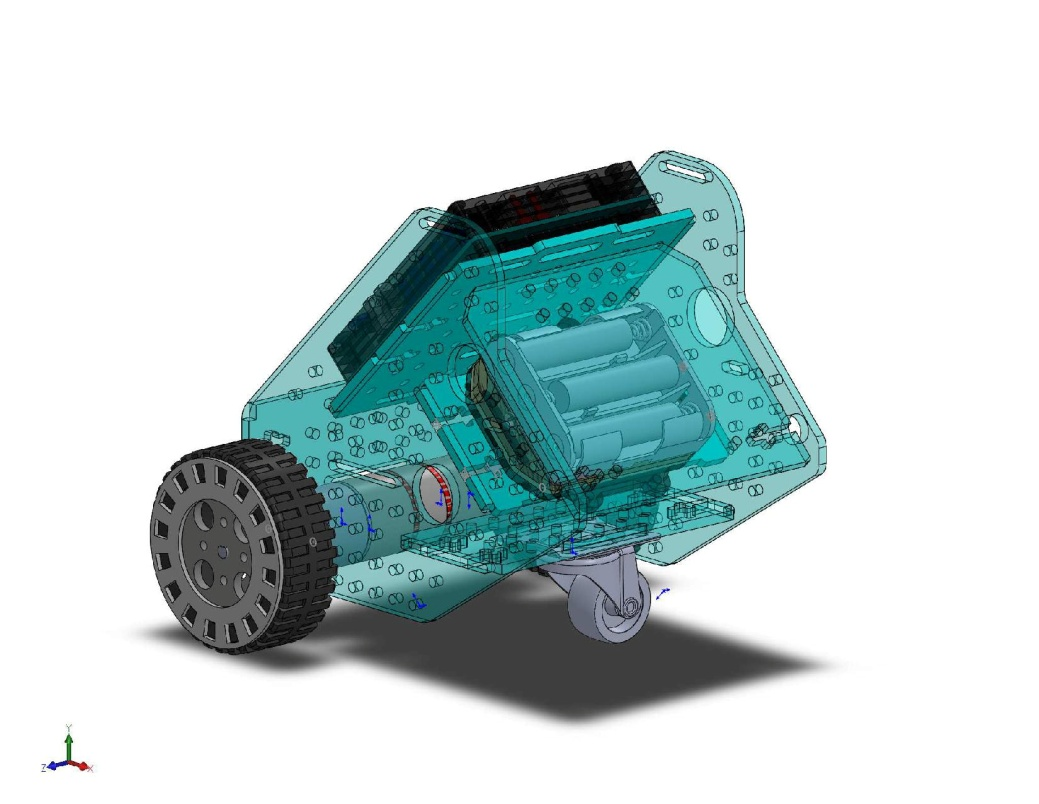
\includegraphics[width=0.7\linewidth]{./robo}
\caption{Rear view of the mobile robot used}
\label{fig:robo}
\end{figure}

The programming environment is based on the Multiplo Development Platform \cite{duinobot_multiplo_2016}, which is also a modified version of the Arduino platform, specifically design for it's use in mobile robot controllers.

%------------------------------------------
\subsection{Kinematic Model}

For the kinematic model, the model proposed by \cite{dudek_computational_2010} was used.
This proposal consists on modeling the differential robot trajectory as a combination of circular trajectories, where the radius, center of rotation and period are a dependent on the instantaneous velocity of both wheels.

\begin{figure}[h]
\centering
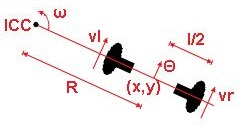
\includegraphics[width=0.6\linewidth]{./parametros}
\caption{Proposed trajectory model}
\label{fig:parametros}
\end{figure}

In this model, the matrix equation \eqref{eq:matriz} that describes this circular trajectory is applied in the central point of the axis between the wheels: by starting on any given point ($x,y,\Theta$) one can obtain it's final location ($x^{'},y^{'},\Theta^{'}$) via this equation:

\small
\begin{equation}
\label{eq:matriz}
\begin{bmatrix}
x^{'}\\
y^{'}\\
\Theta^{'}
\end{bmatrix}=
\begin{bmatrix}
\cos\left(\omega\delta t\right) && -\sin\left(\omega\delta t\right) && 0\\
\sin\left(\omega\delta t\right) && \cos\left(\omega\delta t\right) && 0\\
0 && 0 && 1
\end{bmatrix}
\begin{bmatrix}
x-\text{ICC}_x\\
y-\text{ICC}_y\\
\Theta
\end{bmatrix}+
\begin{bmatrix}
\text{ICC}_x\\
\text{ICC}_y\\
\omega\delta t
\end{bmatrix}
\end{equation}
\normalsize

where $R$ (radius from the center of rotation) and $\omega\delta t$ can be obtained from the following expressions:

\begin{equation}
R = \frac{l}{2}\cdot\frac{n_l + n_r}{n_l - n_r},
\label{radio}
\end{equation}

\begin{equation}
\omega\delta t=\frac{\left(n_r - n_l\right)\cdot\text{step}}{l},
\label{omega}
\end{equation}

In these expressions, the values $n_l$ and $n_r$ are the measured counts from the rotary encoders on the left and right wheels respectively.
The $step$ parameter, meanwhile, is the constant arc length between two slits in the encoder.
By multiplying $n_x$ by $step$, the instantaneous velocity on a wheel can be easily calculated.

To obtain the instant center of rotation (ICC), expression \ref{eq:icc} is used:

\begin{equation}
\label{eq:icc}
\text{ICC}=\left[x-R\sin\Theta , y+R\cos\Theta\right].
\end{equation}

To verify this kinematic model, the robot was programmed to make a simple circular trajectory.
Data input was sent to a laboratory computer, to be analyzed via Matlab.
The desired velocities of both wheels need to be inputed in the program as a percentage of the motors max velocity, for quick testing purposes, velocity is not controlled with a closed-loop scheme in this project. 

%------------------------------------------
\subsection{Dynamic Model}

To obtain the vehicle's dynamic response, a model proposed by \cite{ivanjko_modelling_2010} was used, which makes an analysis based on Lagrange energy considerations.

In a differential robot, it's movement is restricted inside a planar surface.
Therefore, the energy balance is obtained as the sum of partial kinetic energy, since potential energy variations remain null.
This energy is therefore calculated as the sum of both translation and rotation energy of the mobile robot, as well as the energy of each wheel.

In this model, the final equations that explain the torque each wheel receives, is a function of the robot's own parameters, friction with the surface, acceleration function, and the velocities applied to each wheel.
The equations are as follows:

\begin{align}
D_{11}\ddot{\Theta}_r+D_{12}\ddot{\Theta}_l+\beta\dot{\Theta}_r&=\tau_r,
\label{ec_din_1}\\
D_{21}\ddot{\Theta}_r+D_{22}\ddot{\Theta}_l+\beta\dot{\Theta}_l&=\tau_l,
\label{ec_din_2}
\end{align}

Where parameters $D_{11}$, $D_{12}$, $D_{21}$, $D_{22}$, are obtained in expressions:

\begin{align}
D_{11}=D_{22}&=\left[\frac{mr^2}{4}+\frac{\left(I_A + md^2\right)r^2}{b^2}+I_0\right],\\
D_{21}=D_{12}&=\left[\frac{mr^2}{4}-\frac{\left(I_A + md^2\right)r^2}{b^2}\right],
\end{align}

Where parameter $m$ corresponds to the robot's total mass, $r$ is the wheels' radius, $d$ the distance between the middle of the wheels' axis and the robot's center of mass, $b$ the distance between wheels, $I_O$ the moment of inertia of the wheel-motor set, and $I_A$ the moment of inertia of the whole robot along the center of rotation ICC.

By analyzing equations \ref{ec_din_1} and \ref{ec_din_2}, one can see that the result of the torque equations are dependent on the influences of both the acceleration function and the velocity function.
This means that, if discontinuities in those functions are present, this will directly affect the torque functions.
At the same time, if the RMS values of acceleration functions are reduced, the RMS torque will also be reduced, requiring less from the motors, and smaller motors could be used instead.

For these reasons, it's important to analyze in detail the diverse number of interpolators available that allow us to satisfy the desired trajectory requirements.

%-----------------------------------
\subsection{Trajectory Interpolators}

There are many different ways of obtaining any given trajectory, depending on the desired velocity and acceleration on every point.
An Interpolator is a mathematical function that states position as a function of time (in the case of polynomial interpolators), or acceleration as a function of time (in cycloidal interpolators).
The selected interpolator will then be defined depending on the form of the controlled velocity or acceleration.
A detailed description of the most commonly used interpolators can be found in \cite{canini_controllo_2003}, most notably, polynomial interpolators of any order, or many other different shapes (cycloidal, S-type, trapezoidal, etc.); each one of these has different characteristics and their own advantages and disadvantages (continuity, diminution of RMS values, etc).

%-----------------------------------
\subsubsection{\textbf{3rd order polynomial interpolators:}}

In this case, the position as a function of time is:
\begin{align}
x(t) = a_0 + a_1 \cdot t + a_2 \cdot t^2 + a_3 \cdot t^3.
\end{align}

It's derivative, velocity, is a quadratic function, forming a parabola where it's vertex is found in the middle point of the trajectory.
Acceleration on the other hand, is a linear function with a set slope, therefore presenting discontinuities at both the start and the end of the trajectory.
The parameters $a_n$ can be obtained by knowing the desired initial and final positions, and by defining initial and final velocities.
The $3^{rd}$ order interpolator can be determined by the desired positions and velocities, but the desired acceleration cannot be set, and remains discontinuous.

%-----------------------------------
\subsubsection{\textbf{5th order polynomial interpolators:}}

In this case, the position as a function of time is:

\small
\begin{align}
x(t) = a_0 + a_1 \cdot t + a_2 \cdot t^2 + a_3 \cdot t^3 + a_4 \cdot t^4 + a_5 \cdot t^5.
\end{align}
\normalsize

This interpolator is very similar to the $3^{rd}$ order interpolator, but in this case, not only the initial and final positions can be chosen, but also the initial and final velocity, and acceleration.
It also guarantees that every control variable is completely continuous.

%-----------------------------------
\subsubsection{\textbf{Cycloidal Interpolator}}

Contrasting the polynomial interpolators, this kind needs to be defined as a specific continuous acceleration function.
In this case, velocity and position will be determined via multiple integrations of this acceleration function.

In this case, the acceleration as a function of time is:

\begin{align}
\ddot{x}_{(t)} = \dfrac{ x_{(t_f)} - x_{(t_i)} }{ {(t_f - t_i)}^{2} } \cdot 2 \cdot \pi \cdot sin( \dfrac{ 2 \cdot \pi \cdot t }{ t_f - t_i } ).
\end{align}

This interpolator allows to define the initial and final position, as well as acceleration and velocity, which are all continuous, just like in the $5^{th}$ order interpolator.
The main feature of this interpolator is that acceleration follows a sinusoidal form, which guarantees no discontinuities and a smooth evolution.
This is highly important, as it minimizes mechanic vibrations, especially in electric motors with loose mechanic couplings.

%-----------------------------------

\subsection{Comparison Between Results}

It is useful to compare the diverse interpolators used, by showing their results in a table, and also comparing them with the result without using interpolators (this function is called a constant acceleration function).
The compared values are maximum velocity, maximum acceleration, and RMS acceleration, all of them normalized, as seen in table \ref{table:Interpoladores}.
This makes the comparison between interpolators easier.

\small
\begin{table}[h]
\caption{Comparative results of various interpolators}
\label{table:Interpoladores}
\begin{tabular}{|p{1.5cm}|p{1.5cm}|p{1.5cm}|p{1.5cm}|}
\hline
& Norm. Maximum Velocity & Norm. Maximum Acceleration & Norm. RMS Acceleration\\
\hline
Constant Acceleration & \SI{1}{\metre \per \second} & \SI{1}{\metre \per \second \squared} & \SI{1}{\metre \per \second \squared}\\
\hline
$3^{rd}$ order polynomial & \SI{0.75}{\metre \per \second} & \SI{1.5}{\metre \per \second \squared} & \SI{0.87}{\metre \per \second \squared}\\
\hline
$5^{th}$ order polynomial & \SI{0.94}{\metre \per \second} & \SI{1.44}{\metre \per \second \squared} & \SI{1.03}{\metre \per \second \squared}\\
\hline
Cycloidal & \SI{1}{\metre \per \second} & \SI{1.57}{\metre \per \second \squared} & \SI{1.11}{\metre \per \second \squared}\\
\hline
\end{tabular}
\end{table}
\normalsize

%------------------------------------------
\subsection{Velocity Measurements}

To verify the models under study, it was necessary to measure the robot's position and velocity.
To that end, the robot has a set of optical rotary encoders.
These encoders consist on a continuous light source, and an optic receptor that measures the light reflected on a white slitted disk that spins along the wheel, where light will be reflected on the disk, except on black spaces.
This allows the measurement of the wheel's rotation speed, by measuring the time between the reflected light samples.

In practice, a 16-division encoder was implemented, using a CNY17 (Fig.:\ref{fig:encoder}) sensor.
This way, 16 pulses will be measured in each full rotation.
These pulses were measured by programming the micro-controller's timer interrupt, to measure continuously every $1 ms$, in other words, the encoders have a sampling frequency of $1 KHz$, a value higher than the maximum frequency of the pulses of light, when the wheel spins at it's maximum frequency.

Since the measurement disk contains 16 slits, each pulse of light translates to a 22.5º angle movement that, along with the time measured between pulses allows to calculate the rotation speed on each wheel at any given time.
By multiplying this rotation speed by the wheel's radius, the instantaneous speed can be obtained.

\begin{figure}[h]
\centering
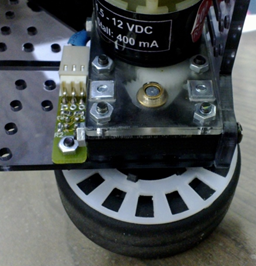
\includegraphics[width=0.6\linewidth]{./encoder}
\caption{Optical encoders on the robot's wheel}
\label{fig:encoder}
\end{figure}

Because of the looseness of the wheel, the motor-wheel set sometimes moves farther from the sensor, and sometimes moves closer.
Therefore, the optical signal measured has not constant peak values, and this makes it difficult to set a fixed threshold to measure the rotation speed.
To solve this issue, instead of measuring the period of the signal, the signal is instead filtered, to contain a null mean value, and then zero-crossings are counted instead.
This greatly simplifies the measurement technique, and it provides no additional error.

%-----------------------------------
\section{Discussion and Results}
%-----------------------------------

To verify the kinematic model, the theoretical velocities for the wheels were set, so they would make a circular clockwise trajectory.
By solving equations \ref{radio} and \ref{omega}, comfortable radius and period values were chosen; given this condition, the left wheel would need a higher velocity, since it would be farther to the center of rotation.

Two similar studies, with the same input values were made:
Firstly, the robot was activated in a way it's wheels would not touch the ground.
In this way, the robot was guaranteed not to have any friction with the surface, and no opposing torque generated by it's own mass, this was made to minimize slip, and so that the speed would not be altered.
This consideration would make the kinematic model more accurate in it's simplified hypothesis.
With these conditions, the wheels' speeds were measured, and their trajectory found in figure \ref{fig:tray} was obtained.
The initial analysis shows a different result that was expected, due to mechanical imprecision of the mobile parts and bad implementation of the motor driver's libraries.
A circular trajectory, however, was obtained, but with a significantly smaller radius.

Then, a similar test was made, with the robot on the ground, on a perfectly planar surface.
As was expected, and seen in figure \ref{fig:tray}, the obtained results were also unsatisfactory and different to both the previous test, and the theoretic model.
In this case, even more factors can cause these discrepancies, for example slip, friction, and such, which make the simplified models not work as expected.
However, this data obtained was used to obtain new calibration coefficients, to apply to each independent wheel, with the objective of making the desired trajectories closer to those predicted by the mathematical modeling.
These coefficients are used as a correction value for the open-loop speed control.

\begin{figure}[h]
\centering
\newlength\figureheight
\newlength\figurewidth
\setlength\figureheight{\columnwidth} \setlength\figurewidth{\columnwidth}
\noindent\resizebox{0.9\columnwidth}{!}{
\begin{tikzpicture}[trim axis left, trim axis right]

\begin{axis}[%
width=\figurewidth,
height=\figureheight,
at={(0\figurewidth,0\figureheight)},
scale only axis,
separate axis lines,
tick label style={/pgf/number format/fixed},
every outer x axis line/.append style={black},
every x tick label/.append style={font=\color{black}},
xmin=-0.165,
xmax=0.165,
xlabel={Metros},
xmajorgrids,
every outer y axis line/.append style={black},
every y tick label/.append style={font=\color{black}},
ymin=-0.165,
ymax=0.165,
ylabel style={rotate=-90,xshift=-0.7cm},
ymajorgrids,
axis background/.style={fill=white}
]
\addplot [color=blue,only marks,mark=x,mark options={solid},forget plot]
  table[row sep=crcr]{%
0.15	0\\
0.149988156630572	0.00188490598250289\\
0.149893420896088	0.00565352740049018\\
0.149573835039092	0.0112990208291899\\
0.148817205197172	0.0187999850346456\\
0.147343087609303	0.0281071971878587\\
0.144807245824991	0.0391262259434845\\
0.140810078648081	0.0516964384761775\\
0.134910787734956	0.0655673649976399\\
0.126649188825302	0.0803740192468495\\
0.115576986416368	0.0956135984623034\\
0.101299921218154	0.110626967603726\\
0.0835313424732281	0.124589384879372\\
0.0621563371489925	0.136515895602749\\
0.0373034830747281	0.145287474169295\\
0.00941857792939688	0.149704009264241\\
-0.0206685436026958	0.148569213854498\\
-0.0516964384761777	0.140810078648081\\
-0.0819591520101405	0.125629206006321\\
-0.109345294113212	0.102682065889303\\
-0.13144600200658	0.0722630511152572\\
-0.145744759937201	0.0354748495535586\\
-0.149893420896088	-0.00565352740049031\\
-0.142064745749212	-0.0481415414710815\\
-0.121352549156242	-0.0881677878438711\\
-0.088167787843871	-0.121352549156242\\
-0.0445562372365553	-0.143229681711997\\
0.00565352740049011	-0.149893420896089\\
0.0569668643282701	-0.138761581025169\\
0.102682065889303	-0.109345294113212\\
0.135724057869903	-0.0638668937347611\\
0.149810543490903	-0.00753664772696559\\
0.140810078648081	0.0516964384761774\\
0.108046353733186	0.104047995871921\\
0.0552186829027014	0.139466472883237\\
-0.00941857792939727	0.14970400926424\\
-0.073909101232244	0.130527563200428\\
-0.124589384879372	0.0835313424732277\\
-0.149041696578001	0.0169284577310217\\
-0.139466472883238	-0.0552186829027022\\
-0.0956135984623034	-0.115576986416369\\
-0.0262534588462913	-0.147684650179381\\
0.0516964384761776	-0.140810078648081\\
0.116769345235053	-0.0941537041936051\\
0.148817205197171	-0.0187999850346456\\
0.135724057869902	0.0638668937347609\\
0.0787761944941938	0.127649172269204\\
-0.0056535274004908	0.149893420896088\\
-0.0896857474586284	0.120235047730631\\
-0.142658477444273	0.0463525491562415\\
-0.142658477444273	-0.0463525491562427\\
-0.0866359055133401	-0.122450887607578\\
0.00565352740049033	-0.149893420896089\\
0.0970583942354168	-0.114366376651717\\
0.147343087609303	-0.0281071971878588\\
0.131446002006579	0.0722630511152571\\
0.0534617818069872	0.140149341368492\\
-0.0516964384761779	0.140810078648081\\
-0.132343683965243	0.0706055898247994\\
-0.145287474169295	-0.0373034830747287\\
-0.0803740192468491	-0.126649188825303\\
0.0299564970771614	-0.146978257857637\\
0.124589384879372	-0.0835313424732282\\
0.146978257857637	0.0299564970771611\\
0.0803740192468494	0.126649188825302\\
-0.0373034830747284	0.145287474169294\\
-0.132343683965243	0.0706055898247994\\
-0.140810078648081	-0.051696438476178\\
-0.0534617818069871	-0.140149341368492\\
0.0722630511152578	-0.131446002006579\\
0.147343087609303	-0.0281071971878582\\
0.114366376651717	0.097058394235417\\
-0.00565352740049099	0.149893420896088\\
-0.122450887607578	0.0866359055133389\\
-0.142658477444273	-0.0463525491562435\\
-0.046352549156241	-0.142658477444274\\
0.0896857474586288	-0.120235047730632\\
0.149893420896089	0.00565352740048995\\
0.0787761944941954	0.127649172269204\\
-0.0638668937347598	0.135724057869903\\
-0.14881720519717	0.0187999850346452\\
-0.094153704193603	-0.116769345235054\\
0.0516964384761797	-0.140810078648081\\
0.147684650179382	-0.0262534588462905\\
0.0956135984623045	0.115576986416369\\
-0.0552186829027007	0.139466472883238\\
-0.149041696578	0.0169284577310227\\
-0.0835313424732279	-0.124589384879372\\
0.073909101232244	-0.130527563200429\\
0.149704009264241	0.00941857792939722\\
0.0552186829027014	0.139466472883238\\
-0.104047995871921	0.108046353733185\\
-0.140810078648081	-0.0516964384761783\\
-0.00753664772696475	-0.149810543490903\\
0.135724057869904	-0.0638668937347612\\
0.109345294113213	0.102682065889303\\
-0.0569668643282691	0.138761581025169\\
-0.149893420896088	-0.00565352740048949\\
-0.0445562372365543	-0.143229681711996\\
0.121352549156243	-0.0881677878438699\\
0.121352549156242	0.0881677878438721\\
-0.0481415414710817	0.142064745749211\\
-0.149893420896087	-0.0056535274004917\\
-0.0354748495535555	-0.145744759937201\\
0.131446002006582	-0.0722630511152551\\
0.102682065889303	0.109345294113213\\
-0.0819591520101412	0.125629206006321\\
-0.140810078648079	-0.0516964384761789\\
0.0206685436026983	-0.148569213854498\\
0.149704009264242	-0.0094185779293956\\
0.0373034830747268	0.145287474169294\\
-0.136515895602749	0.0621563371489893\\
-0.0835313424732242	-0.124589384879374\\
0.11062696760373	-0.101299921218152\\
0.115576986416367	0.0956135984623052\\
-0.0803740192468511	0.1266491888253\\
-0.134910787734953	-0.0655673649976432\\
0.0516964384761814	-0.140810078648081\\
0.144807245824992	0.0391262259434859\\
-0.0281071971878591	0.147343087609303\\
-0.14881720519717	-0.0187999850346471\\
0.0112990208291931	-0.149573835039091\\
0.14989342089609	0.00565352740049296\\
-0.00188490598250418	0.149988156630573\\
-0.149999999999999	-1.73038666728687e-15\\
3.03704771181041e-15	-0.149999999999999\\
0.149988156630574	0.00188490598250505\\
-0.00565352740049035	0.149893420896089\\
-0.149573835039092	-0.0112990208291901\\
0.0187999850346467	-0.148817205197171\\
0.147343087609303	0.0281071971878603\\
-0.039126225943486	0.144807245824991\\
-0.14081007864808	-0.0516964384761785\\
0.0655673649976414	-0.134910787734955\\
0.126649188825302	0.0803740192468508\\
-0.0956135984623044	0.115576986416369\\
-0.101299921218153	-0.110626967603726\\
0.124589384879372	-0.0835313424732283\\
0.0621563371489934	0.136515895602749\\
-0.145287474169293	0.0373034830747274\\
-0.00941857792939545	-0.149704009264241\\
0.148569213854498	0.0206685436026961\\
-0.0516964384761773	0.140810078648081\\
-0.125629206006323	-0.0819591520101398\\
0.10934529411321	-0.102682065889306\\
0.0722630511152583	0.131446002006577\\
-0.145744759937201	0.0354748495535577\\
0.00565352740049201	-0.149893420896088\\
0.142064745749214	0.0481415414710815\\
-0.0881677878438688	0.121352549156243\\
-0.0881677878438684	-0.121352549156241\\
0.143229681711998	-0.0445562372365517\\
-0.00565352740048871	0.149893420896092\\
-0.138761581025168	-0.0569668643282661\\
0.102682065889304	-0.109345294113208\\
0.0638668937347602	0.135724057869906\\
-0.149810543490901	0.00753664772696471\\
0.0516964384761806	-0.14081007864808\\
0.108046353733187	0.104047995871922\\
-0.139466472883236	0.0552186829027004\\
0.00941857792940338	-0.149704009264239\\
0.130527563200433	0.0739091012322472\\
-0.124589384879368	0.0835313424732301\\
-0.0169284577310168	-0.149041696577999\\
0.13946647288324	0.0552186829027067\\
-0.115576986416366	0.0956135984623084\\
-0.0262534588462909	-0.147684650179377\\
0.140810078648084	0.0516964384761801\\
-0.116769345235051	0.094153704193609\\
-0.0187999850346417	-0.148817205197167\\
0.135724057869908	0.0638668937347643\\
-0.127649172269198	0.0787761944942008\\
0.00565352740049338	-0.149893420896083\\
0.120235047730635	0.0896857474586326\\
-0.142658477444269	0.0463525491562439\\
0.046352549156247	-0.142658477444271\\
0.0866359055133447	0.12245088760758\\
-0.149893420896083	-0.00565352740048905\\
0.0970583942354238	-0.114366376651712\\
0.0281071971878644	0.147343087609308\\
-0.131446002006574	-0.0722630511152526\\
0.140149341368498	-0.0534617818069824\\
-0.0516964384761736	0.140810078648085\\
-0.0706055898247896	-0.13234368396524\\
0.145287474169302	0.0373034830747345\\
-0.126649188825295	0.0803740192468521\\
0.0299564970771723	-0.146978257857632\\
0.0835313424732316	0.124589384879379\\
-0.146978257857631	-0.0299564970771581\\
0.126649188825309	-0.0803740192468432\\
-0.0373034830747246	0.145287474169299\\
-0.0706055898247903	-0.13234368396524\\
0.140810078648084	0.0516964384761884\\
-0.140149341368489	0.0534617818069906\\
0.072263051115265	-0.131446002006571\\
0.028107197187858	0.14734308760931\\
-0.114366376651708	-0.0970583942354154\\
0.149893420896095	0.00565352740049944\\
-0.122450887607573	0.0866359055133425\\
0.0463525491562525	-0.142658477444266\\
0.0463525491562426	0.14265847744428\\
-0.12023504773062	-0.089685747458629\\
0.149893420896094	0.00565352740050773\\
-0.127649172269206	0.0787761944941853\\
0.0638668937347745	-0.135724057869898\\
0.0187999850346437	0.148817205197174\\
-0.0941537041935954	-0.116769345235056\\
0.140810078648084	0.051696438476184\\
-0.147684650179377	0.0262534588462862\\
0.115576986416378	-0.095613598462296\\
-0.0552186829027063	0.139466472883235\\
-0.0169284577310029	-0.149041696578001\\
0.0835313424732175	0.124589384879383\\
-0.130527563200422	-0.0739091012322511\\
0.149704009264241	0.00941857792940888\\
-0.13946647288324	0.055218682902697\\
0.104047995871927	-0.108046353733178\\
-0.0516964384761844	0.140810078648081\\
-0.0075366477269541	-0.1498105434909\\
0.0638668937347504	0.135724057869911\\
-0.109345294113199	-0.102682065889312\\
0.138761581025162	0.056966864328292\\
-0.149893420896089	-0.00565352740049735\\
0.143229681711999	-0.0445562372365381\\
-0.121352549156249	0.088167787843869\\
0.0881677878438779	-0.12135254915623\\
-0.0481415414710927	0.142064745749214\\
0.00565352740050146	-0.149893420896081\\
0.035474849553543	0.145744759937211\\
-0.072263051115242	-0.131446002006582\\
0.102682065889285	0.109345294113234\\
-0.125629206006317	-0.0819591520101449\\
0.140810078648072	0.0516964384761992\\
-0.148569213854501	-0.0206685436026993\\
0.149704009264237	-0.00941857792937601\\
-0.145287474169302	0.0373034830747243\\
0.136515895602751	-0.0621563371489705\\
-0.124589384879386	0.0835313424732224\\
0.110626967603736	-0.101299921218129\\
-0.0956135984623275	0.115576986416361\\
0.0803740192468572	-0.126649188825287\\
-0.0655673649976621	0.134910787734954\\
0.0516964384761838	-0.14081007864807\\
-0.0391262259435065	0.144807245824993\\
0.0281071971878661	-0.147343087609295\\
-0.0187999850346704	0.148817205197175\\
0.0112990208292018	-0.149573835039085\\
-0.00565352740052136	0.149893420896093\\
0.00188490598252291	-0.149988156630566\\
-2.42540362793697e-14	0.150000000000006\\
1.48335467710866e-14	-0.149999999999994\\
-0.00188490598252386	0.149988156630578\\
0.00565352740050375	-0.149893420896082\\
-0.0112990208292113	0.149573835039097\\
0.0187999850346615	-0.148817205197163\\
-0.0281071971878841	0.147343087609305\\
0.0391262259435061	-0.144807245824979\\
-0.0516964384762096	0.140810078648077\\
0.0655673649976531	-0.134910787734941\\
-0.0803740192468747	0.126649188825296\\
0.0956135984623113	-0.115576986416351\\
-0.110626967603747	0.101299921218144\\
0.124589384879376	-0.0835313424732065\\
-0.136515895602766	0.0621563371489771\\
0.145287474169294	-0.0373034830746995\\
-0.14970400926425	0.00941857792937329\\
0.148569213854486	0.0206685436027332\\
-0.14081007864808	-0.0516964384761927\\
0.125629206006301	0.0819591520101692\\
-0.102682065889294	-0.109345294113218\\
0.0722630511152301	0.131446002006599\\
-0.0354748495535439	-0.145744759937198\\
-0.00565352740052268	0.149893420896097\\
0.0481415414710999	-0.142064745749194\\
-0.0881677878439041	0.121352549156233\\
0.121352549156256	-0.0881677878438332\\
-0.143229681712009	0.0445562372365402\\
0.149893420896083	0.00565352740052881\\
-0.138761581025164	-0.0569668643282812\\
0.10934529411319	0.102682065889334\\
-0.0638668937347422	-0.135724057869902\\
0.00753664772693312	0.149810543490917\\
0.0516964384762014	-0.140810078648059\\
-0.10404799587195	0.108046353733175\\
0.139466472883248	-0.0552186829026539\\
-0.149704009264241	-0.00941857792941241\\
0.130527563200412	0.0739091012322848\\
-0.0835313424732071	-0.124589384879372\\
0.0169284577309767	0.149041696578026\\
0.0552186829027271	-0.139466472883204\\
-0.115576986416389	0.0956135984623038\\
0.147684650179386	-0.0262534588462351\\
-0.140810078648072	-0.0516964384761722\\
0.0941537041935801	0.116769345235107\\
-0.0187999850346226	-0.148817205197139\\
-0.0638668937348008	0.135724057869926\\
0.127649172269209	-0.0787761944941312\\
-0.149893420896102	-0.00565352740050008\\
0.120235047730592	0.0896857474586896\\
-0.0463525491562308	-0.142658477444247\\
-0.046352549156297	0.142658477444299\\
0.122450887607568	-0.0866359055132815\\
-0.149893420896116	-0.00565352740049251\\
0.114366376651669	0.0970583942354673\\
-0.0281071971878484	-0.147343087609287\\
-0.0722630511153112	0.131446002006586\\
0.14014934136849	-0.0534617818069212\\
-0.140810078648083	-0.0516964384761913\\
0.0706055898247541	0.132343683965279\\
0.0373034830747524	-0.145287474169267\\
-0.126649188825327	0.080374019246842\\
0.146978257857625	0.0299564970772203\\
-0.0835313424732064	-0.124589384879364\\
-0.0299564970772103	0.146978257857659\\
0.12664918882531	-0.0803740192467879\\
-0.1452874741693	-0.0373034830747493\\
0.0706055898247426	0.132343683965288\\
0.0516964384761908	-0.140810078648041\\
-0.140149341368532	0.0534617818069754\\
0.131446002006535	0.0722630511153096\\
-0.0281071971878447	-0.147343087609293\\
-0.097058394235466	0.114366376651711\\
0.14989342089607	0.00565352740055342\\
-0.086635905513324	-0.122450887607579\\
-0.0463525491563121	0.142658477444285\\
0.142658477444265	-0.0463525491561682\\
-0.120235047730627	-0.0896857474586274\\
-0.00565352740055675	0.149893420896123\\
0.127649172269196	-0.0787761944941257\\
-0.135724057869915	-0.0638668937347678\\
0.0187999850345779	0.148817205197206\\
0.11676934523506	-0.0941537041935414\\
-0.140810078648087	-0.0516964384761896\\
0.0262534588462159	0.147684650179427\\
0.115576986416378	-0.0956135984622263\\
-0.13946647288324	-0.0552186829027014\\
0.0169284577309549	0.149041696578051\\
0.12458938487937	-0.0835313424731481\\
-0.130527563200434	-0.0739091012322424\\
-0.00941857792946596	0.149704009264277\\
0.139466472883236	-0.0552186829026171\\
-0.108046353733173	-0.104047995871914\\
-0.0516964384762546	0.140810078648108\\
0.149810543490881	-0.00753664772686331\\
-0.0638668937347412	-0.13572405786987\\
-0.102682065889367	0.109345294113231\\
0.138761581025121	0.0569668643283631\\
0.00565352740051135	-0.14989342089604\\
-0.143229681712035	0.0445562372365581\\
0.0881677878438053	0.121352549156326\\
0.0881677878438876	-0.121352549156158\\
-0.142064745749224	-0.0481415414710881\\
-0.00565352740058054	0.149893420896136\\
0.145744759937175	-0.035474849553459\\
-0.0722630511152485	-0.131446002006559\\
-0.109345294113279	0.102682065889312\\
0.125629206006261	0.0819591520102323\\
0.0516964384761913	-0.140810078648014\\
-0.148569213854529	-0.020668543602703\\
0.00941857792930408	0.149704009264291\\
0.14528747416928	-0.0373034830746216\\
-0.0621563371489661	-0.13651589560273\\
-0.124589384879427	0.0835313424732247\\
0.101299921218088	0.11062696760381\\
0.0956135984623173	-0.115576986416287\\
-0.126649188825302	-0.080374019246852\\
-0.0655673649977162	0.134910787734975\\
0.140810078648038	0.0516964384762788\\
0.0391262259435174	-0.144807245824929\\
-0.147343087609322	-0.028107197187879\\
-0.0187999850347427	0.148817205197208\\
0.149573835039049	0.011299020829293\\
0.00565352740051386	-0.149893420896044\\
-0.149988156630604	-0.00188490598251733\\
-9.32431215572294e-14	0.150000000000046\\
0.149999999999964	1.03262695349122e-13\\
0.00188490598253011	-0.149988156630532\\
-0.149893420896121	-0.00565352740051196\\
-0.0112990208292943	0.149573835039135\\
0.148817205197128	0.0187999850347634\\
0.0281071971878853	-0.147343087609236\\
-0.144807245825012	-0.0391262259434929\\
-0.0516964384762703	0.14081007864811\\
0.134910787734895	0.0655673649977489\\
0.0803740192468672	-0.126649188825215\\
-0.115576986416365	-0.0956135984623043\\
-0.110626967603808	0.101299921218155\\
0.0835313424731344	0.124589384879469\\
0.136515895602748	-0.0621563371488699\\
-0.0373034830746928	-0.145287474169249\\
-0.149704009264277	0.00941857792939041\\
-0.020668543602791	0.148569213854546\\
0.14081007864803	0.0516964384762994\\
0.0819591520101658	-0.125629206006225\\
-0.102682065889286	-0.109345294113203\\
-0.131446002006646	0.072263051115253\\
0.0354748495534543	0.145744759937283\\
0.149893420896057	0.00565352740063164\\
0.0481415414711196	-0.142064745749118\\
-0.12135254915623	-0.0881677878438602\\
-0.12135254915631	0.0881677878438817\\
0.0445562372364608	0.143229681712087\\
0.149893420896057	0.00565352740062897\\
0.056966864328311	-0.138761581025076\\
-0.109345294113189	-0.102682065889292\\
-0.13572405786997	0.0638668937347575\\
0.00753664772686099	0.149810543490961\\
0.140810078648014	0.0516964384762876\\
0.104047995871918	-0.108046353733091\\
-0.0552186829026892	-0.139466472883219\\
-0.14970400926428	-0.00941857792941525\\
-0.0739091012323347	0.130527563200439\\
0.0835313424731397	0.124589384879447\\
0.149041696577986	-0.0169284577309134\\
0.0552186829027423	-0.139466472883172\\
-0.0956135984622738	-0.115576986416372\\
-0.147684650179426	0.0262534588462605\\
-0.0516964384762716	0.140810078648091\\
0.0941537041935206	0.116769345235121\\
0.148817205197144	-0.018799985034555\\
0.0638668937347937	-0.135724057869856\\
-0.0787761944941652	-0.12764917226922\\
-0.149893420896112	-0.00565352740053658\\
-0.0896857474587124	0.120235047730614\\
0.0463525491561492	0.142658477444307\\
0.142658477444212	0.0463525491563073\\
0.122450887607562	-0.0866359055132819\\
0.00565352740050093	-0.149893420896079\\
-0.114366376651724	-0.0970583942354481\\
-0.14734308760935	0.0281071971878168\\
-0.0722630511153403	0.131446002006564\\
0.0534617818069006	0.140149341368534\\
0.140810078648029	0.0516964384762552\\
0.132343683965241	-0.0706055898247257\\
0.0373034830747609	-0.145287474169265\\
-0.0803740192468238	-0.126649188825316\\
-0.146978257857644	-0.0299564970771976\\
-0.12458938487942	0.0835313424731999\\
-0.0299564970772383	0.146978257857652\\
0.0803740192467801	0.12664918882536\\
0.145287474169259	0.0373034830748099\\
0.132343683965253	-0.0706055898247238\\
0.0516964384762102	-0.140810078648031\\
-0.0534617818069553	-0.14014934136847\\
-0.131446002006567	-0.0722630511152577\\
-0.147343087609327	0.0281071971878524\\
-0.0970583942354647	0.114366376651725\\
-0.00565352740054735	0.14989342089612\\
0.0866359055132911	0.122450887607637\\
0.142658477444255	0.0463525491563241\\
0.142658477444287	-0.0463525491561601\\
0.0896857474586673	-0.120235047730568\\
0.00565352740054184	-0.14989342089606\\
-0.0787761944941497	-0.127649172269202\\
-0.135724057869876	-0.0638668937347751\\
-0.148817205197171	0.0187999850346274\\
-0.116769345235083	0.0941537041935998\\
-0.0516964384762224	0.140810078648097\\
0.0262534588462443	0.147684650179422\\
0.0956135984622684	0.115576986416436\\
0.139466472883219	0.0552186829027804\\
0.149041696577998	-0.0169284577309415\\
0.124589384879384	-0.0835313424731531\\
0.0739091012322707	-0.13052756320037\\
0.00941857792942824	-0.149704009264196\\
-0.0552186829026725	-0.139466472883207\\
-0.108046353733166	-0.104047995871903\\
-0.140810078648079	-0.051696438476171\\
-0.149810543490918	0.00753664772696952\\
-0.135724057869935	0.0638668937347691\\
-0.102682065889352	0.109345294113232\\
-0.0569668643283264	0.138761581025201\\
-0.00565352740054888	0.149893420896133\\
0.0445562372364982	0.143229681712054\\
0.0881677878438216	0.121352549156315\\
0.121352549156202	0.0881677878439527\\
0.142064745749182	0.0481415414711687\\
0.149893420896073	0.00565352740057983\\
0.145744759937194	-0.0354748495534699\\
0.131446002006579	-0.0722630511151709\\
0.109345294113217	-0.102682065889221\\
0.0819591520101512	-0.125629206006246\\
0.0516964384761912	-0.140810078648011\\
0.0206685436027105	-0.148569213854433\\
-0.00941857792938201	-0.149704009264182\\
-0.0373034830747147	-0.145287474169244\\
-0.0621563371489812	-0.136515895602705\\
-0.0835313424732197	-0.124589384879333\\
-0.10129992121815	-0.110626967603692\\
-0.115576986416368	-0.0956135984622727\\
-0.126649188825304	-0.0803740192468207\\
-0.134910787734961	-0.0655673649976129\\
-0.14081007864809	-0.0516964384761523\\
-0.144807245825003	-0.03912622594346\\
-0.147343087609318	-0.0281071971878347\\
-0.148817205197189	-0.0187999850346221\\
-0.149573835039111	-0.0112990208291664\\
-0.149893420896107	-0.00565352740046662\\
-0.149988156630592	-0.00188490598247941\\
-0.15000000000002	2.35332586751014e-14\\
-0.15000000000002	2.35699980790758e-14\\
};
\addplot [color=red,only marks,mark=x,mark options={solid},forget plot]
  table[row sep=crcr]{%
-0.121239602002359	0.00920097104914458\\
-0.11846251995298	0.0273921581538884\\
-0.109246081852831	0.0533759549023928\\
-0.0883443340391121	0.0835402753474245\\
-0.0511957777552311	0.110284592314497\\
0.00241476733279171	0.121564254041499\\
0.0635609920758673	0.103651817390093\\
0.111279599181233	0.0489954055805428\\
0.11728125695835	-0.0320750016088409\\
0.063177001101318	-0.1038863104253\\
-0.0343979052076327	-0.116621109063773\\
-0.113137549457316	-0.0445375556663269\\
-0.0996828619501075	0.0696205860028018\\
0.0120547936493123	0.120989176838303\\
0.114817001372414	0.040009438358776\\
0.0777859051559371	-0.0934507994669349\\
-0.0680005820920238	-0.100794939342626\\
-0.112636163402002	0.0457907595046784\\
0.03061114937015	0.11767181691542\\
0.119197904526079	-0.0239908007062992\\
-0.0263533637934241	-0.118697932495512\\
-0.115640120616211	0.0375640980965333\\
0.0567323967639393	0.107541313546733\\
0.0903986171787213	-0.0813129077952124\\
-0.105792341801277	-0.0599306213728808\\
-0.0141726163101856	0.120759413334373\\
0.11390046204512	-0.042548604064599\\
-0.0958140931646393	-0.0748555843806963\\
-0.0045441446108065	0.121503290950055\\
0.0957405577041534	-0.0749496135576121\\
-0.120573443085162	-0.015676217162537\\
0.0805178870194798	0.0911074576083429\\
-0.00993327068171414	-0.121181801833037\\
-0.0566267910030636	0.107596958612375\\
0.10063546774555	-0.0682363656239987\\
-0.119599917607606	0.0218988280552056\\
0.120075440332072	0.0191203449497333\\
-0.110962801337172	-0.0497087083049343\\
0.0997511637510137	0.0695226890464989\\
-0.091374502071684	-0.0802147077105535\\
0.0884263069250788	0.0834535032549832\\
-0.0916707049938819	-0.0798760340018356\\
0.100262955435949	0.0687825466901793\\
-0.111507783938494	-0.0484738391615914\\
0.120345290764734	0.0173409905336853\\
-0.119174294173179	0.0241078113951136\\
0.0990957639665662	-0.0704537332284125\\
-0.0538210185203537	0.109027505370752\\
-0.0135157961985927	-0.120834689617907\\
0.0835069109899683	0.0883758721532706\\
-0.121070856272456	-0.0112047634241907\\
0.092611289030898	-0.0787835522553609\\
0.000853940232771515	0.121585236554512\\
-0.099302837238471	-0.07016156696032\\
0.111544359122714	-0.0483896157232177\\
-0.00745129763429652	0.121359701406615\\
-0.109153206366779	-0.0535656279883751\\
0.0851079989735856	-0.0868350590064282\\
0.0637643892888676	0.103526815949084\\
-0.112715529174458	0.0455950484686614\\
-0.0350578836224432	-0.116424412207462\\
0.11697575716423	-0.0331718434488152\\
0.0400787980236017	0.114792808620231\\
-0.108335910911611	0.0551999037036231\\
-0.0766724651386115	-0.0943664773715016\\
0.068820400603655	-0.100236976324559\\
0.118129426252537	0.0287947497850586\\
0.0240628100276592	0.119183388672711\\
-0.0919476307804544	0.0795570999710205\\
-0.117257000779312	-0.0321635621500182\\
-0.0471060497226529	-0.112092457558324\\
0.0508707412412579	-0.110434897779202\\
0.112670712028276	-0.0457056846899714\\
0.116419115803089	0.0350754677454878\\
0.0760651399509389	0.0948566995324094\\
0.0180949790317856	0.120234232628553\\
-0.0360939647772631	0.116107384212183\\
-0.0761152737378984	0.0948164757082993\\
-0.100686970501729	0.0681603472197851\\
-0.113291584452784	0.0441442618481202\\
-0.118556961944525	0.0269804695367269\\
-0.120191541196429	0.0183764084294194\\
-0.120122717768398	0.0188210424225541\\
-0.118250144445315	0.0282949165151601\\
-0.112455475477608	0.0462327264720873\\
-0.0988878310933417	0.0707452883490656\\
-0.0729158910196207	0.097298364830826\\
-0.0313392478531121	0.117480000450881\\
0.0238557596475012	0.119225004481352\\
0.0812104533755917	0.0904906692674365\\
0.118393887370004	0.0276872966422594\\
0.109181507692781	-0.0535079184781926\\
0.0421440591029608	-0.114050766083634\\
-0.0564642140639775	-0.107682363885991\\
-0.119726836683964	-0.0211939505422909\\
-0.0835536177555886	0.0883317152663227\\
0.0366897319849818	0.115920500899573\\
0.12064894057851	0.015084167170279\\
0.0560979455585366	-0.107873627296245\\
-0.0882180556677102	-0.0836736136195067\\
-0.0997879018254549	0.0694699475400053\\
0.0561712512242997	0.107835474208789\\
0.110618573911215	-0.0504700908240404\\
-0.0530622294395111	-0.109398806066823\\
-0.103598980906189	0.0636470746942607\\
0.0807172238866326	0.0909309008531915\\
0.0680538561574522	-0.100758977883058\\
-0.117264284655335	-0.0321369959114162\\
0.0163406838243827	0.120485190019725\\
0.0994615383063509	-0.0699364093993395\\
-0.111791382235772	-0.0478161669287002\\
0.0271684550311572	0.118514024542067\\
0.0726290078423904	-0.0975126975412316\\
-0.120384269132321	0.0170682953869041\\
0.102155453179695	0.0659390805788869\\
-0.0427549737893844	-0.113823157477759\\
-0.024539648699773	0.119086122632444\\
0.0773970829139804	-0.0937730799235269\\
-0.108419160199601	0.0550362122929157\\
0.120491351595235	-0.0162951880225789\\
-0.120637514755399	-0.0151752757990936\\
0.11583149773458	0.0369697591891239\\
-0.11116831108687	-0.0492473915251413\\
0.109518741483568	0.0528142426414806\\
-0.111708159913699	-0.0480102694288757\\
0.116623706428475	0.0343890979937332\\
-0.12107592088241	-0.0111499033365414\\
0.119649223986655	-0.0216278099059721\\
-0.10519888551016	0.0609663304567207\\
0.0709840548354076	-0.0987165787548453\\
-0.0152208268712483	0.120631776043019\\
-0.052681872090867	-0.109582477225783\\
0.108223132380061	0.0554206872908086\\
-0.11775231615098	0.0303000165514383\\
0.0602100385155647	-0.105633565801273\\
0.0426690034337165	0.113855413169121\\
-0.117505993726586	-0.0312416452874241\\
0.0874370299140009	-0.0844894357997248\\
0.0360851963544572	0.11611010966319\\
-0.121097580259563	-0.0109121499813952\\
0.0479427719144753	-0.111737145046284\\
0.0971605280267218	0.0730994579699899\\
-0.0879775725637091	0.0839264302096486\\
-0.075850040273784	-0.0950287869669137\\
0.0959665255007574	-0.0746600625853621\\
0.0805797915581681	0.0910527108568433\\
-0.0790071273320943	0.0924206296920117\\
-0.107135875851928	-0.0574943742237276\\
0.0243957384793097	-0.119115687069281\\
0.119951733328934	-0.0198816657582286\\
0.0692814266416064	0.0999188815211691\\
-0.0525328632930698	0.109653988692475\\
-0.120281640624585	0.0177771170496224\\
-0.0885648360710549	-0.0833064749803093\\
0.00119367053355218	-0.121582375830525\\
0.0837535249795876	-0.0881421920276056\\
0.120455375347297	-0.0165590311274429\\
0.108843973094559	0.054191221456326\\
0.0672451067190057	0.101300516209382\\
0.0168409824487988	0.120416279099202\\
-0.0280001343654398	0.118320291740069\\
-0.0612521075278155	0.105032748632694\\
-0.0826824105634444	0.0891477310163065\\
-0.0946264924013238	0.0763513319972869\\
-0.0996197288567928	0.0697108928678783\\
-0.0991010842832922	0.0704462494091313\\
-0.0929081110748393	0.0784332955985087\\
-0.0793277078178751	0.0921456115845978\\
-0.0557310291879305	0.108063644893145\\
-0.0200628158408422	0.119921567628489\\
0.0265774155824385	0.118647966450741\\
0.0766653384528414	0.0943722673344717\\
0.114177552712854	0.0417993471054414\\
0.117425388924196	-0.0315432559818897\\
0.0705734196619296	-0.099010562058595\\
-0.0176408523369167	-0.120301701113346\\
-0.101396899346321	-0.0670996852816002\\
-0.114958287153048	0.0396016562377783\\
-0.0297216384930124	0.117899631751878\\
0.0889726971172879	0.0828707314412819\\
0.112287147327445	-0.0466400633254547\\
-0.00513134132003322	-0.121479909031062\\
-0.118288497677383	-0.0281341479196617\\
-0.0510708161131517	0.110342515393997\\
0.103164000331909	0.064349731914404\\
0.0692738806646833	-0.0999241133040115\\
-0.10177531876531	-0.0665243072279392\\
-0.0557065451650822	0.108076268383528\\
0.116258989264528	0.0356026175600624\\
0.00518638507838617	-0.121477571476205\\
-0.116595098838328	0.0344859665489936\\
0.0777294324355183	0.0934977769531977\\
0.0468435022676474	-0.112202429818782\\
-0.11999646878332	0.0196098557228607\\
0.0868157749512709	0.0851276698938013\\
0.00809273842260793	-0.121318615829398\\
-0.0915620414064704	0.0800005720943139\\
0.121584556996182	-0.000945760001187922\\
-0.0984747799983588	-0.0713191185181964\\
0.0456801571603643	0.112681064086838\\
0.0118903167748909	-0.121005451649628\\
-0.0588569998253974	0.106393385760069\\
0.0902880015629128	-0.0814357153570421\\
-0.107958233496449	0.05593495134765\\
0.116232069355061	-0.0356904050884539\\
-0.119317766291112	0.0233873814104374\\
0.11993819262258	-0.0199631889327971\\
-0.118864651256466	0.0255908898558944\\
0.11483210056158	-0.0399660811508066\\
-0.104688808424408	0.0618381140771237\\
0.0840193990483104	-0.0878887907841409\\
-0.0487768142926006	0.11137558686446\\
-0.00158848034508918	-0.121577858560393\\
0.0598507109149547	0.105837570668039\\
-0.107915961169256	-0.0560164644265711\\
0.119745994083679	-0.0210854419647577\\
-0.0752817515227446	0.0954796148379614\\
-0.0165954170754394	-0.12045036776212\\
0.103430389373	0.063920681442607\\
-0.111870670607048	0.0476303686723835\\
0.0165408375866518	-0.120457875018073\\
0.100371911555867	0.0686234532252556\\
-0.101462725433144	0.0670001067880956\\
-0.0326503158864119	-0.117122396809727\\
0.121510015747781	-0.00436062322514709\\
-0.0150841671703178	0.120648940578505\\
-0.118945222404309	-0.0252137468284091\\
0.0262547512003186	-0.118719783529735\\
0.12021090278275	0.0182493236612734\\
-0.000964123891844183	0.121584412763557\\
-0.11890316765769	0.0254113298137854\\
-0.0588007485090257	-0.106424484667374\\
0.0779621993187155	-0.0933037750539955\\
0.117797946394114	0.0301221311873373\\
0.032561856858039	0.11714702061894\\
-0.0785595170827779	0.0928014075198132\\
-0.121535232763791	-0.00358972965399932\\
-0.0800973328661091	-0.0914774083021236\\
0.00330519507614283	-0.121543303589488\\
0.0781241445284603	-0.0931682188497449\\
0.116915442514637	-0.0333838024129115\\
0.118074851944667	0.0290177238973485\\
0.0942099450464677	0.0768647202315812\\
0.0602897948083826	0.105588065631968\\
0.0273563721947491	0.118470789067517\\
0.001313033157363	0.121581145355131\\
-0.0157126388163481	0.120568702171686\\
-0.023468472886047	0.119301842996387\\
-0.0221426483249708	0.119555016988391\\
-0.0116892596772319	0.121025039434557\\
0.00805609058533325	0.121321054918009\\
0.0364708115608133	0.115989563608255\\
0.0705210695152752	0.0990478556878414\\
0.102871364434589	0.0648165205893047\\
0.121020616997718	0.0117349573254223\\
0.109764825964699	-0.0523008789876134\\
0.0592583156782297	-0.106170386572325\\
-0.022214873733844	-0.119541617635563\\
-0.099063830199034	-0.0704986277046205\\
-0.118501701960133	0.0272221526424629\\
-0.0501273432311802	0.110774313008572\\
0.0656997449216884	0.102309542463852\\
0.121276772758263	-0.0086973186257743\\
0.0419114204940615	-0.11413646128257\\
-0.0930205563528913	-0.0782999045831876\\
-0.100413352261773	0.0685628007704677\\
0.0476641599676408	0.111856277501609\\
0.1167757731794	-0.0338691269490538\\
-0.0286073721796213	-0.118174943278659\\
-0.117232677727138	0.0322521043478215\\
0.0445546432396321	0.113130821298737\\
0.103168859668668	-0.0643419408831013\\
-0.0885522526084886	-0.0833198506953783\\
-0.0496919481264403	0.110970307980725\\
0.121580434253884	0.00137730482275616\\
-0.0555105701526193	-0.108177056547444\\
-0.0620435507371484	0.104567187845254\\
0.120963416105649	-0.012310602178178\\
-0.0884073976669142	-0.083473534726294\\
0.00385588938127936	0.121527079611982\\
0.0759719779620774	-0.0949313305840983\\
-0.11734400995831	0.0318446587176221\\
0.116506166773251	0.034785227694253\\
-0.0873284883279749	-0.0846016198916337\\
0.0470806531647737	0.112103126894463\\
-0.00846833558195873	-0.121292976937698\\
-0.0220613850805489	0.11957003909954\\
0.0427033944989667	-0.113842518683501\\
-0.0539280300691886	0.108974614175937\\
0.0566267910030867	-0.107596958612363\\
-0.0510874814553553	0.110334800495974\\
0.0367510063017576	-0.115901089286278\\
-0.0127124753585112	0.120921842246126\\
-0.0209678714674485	-0.119766636957302\\
0.0611648346912357	0.105083595099956\\
-0.0993716703292061	-0.0700640428316929\\
0.120868995064525	0.0132054910559749\\
-0.108281666332982	0.0553062356167053\\
0.0519856693012165	-0.109914462875648\\
0.0348556088257743	0.116485129932203\\
-0.108306715263913	-0.0552571659667713\\
0.111401356353313	-0.0487179306270267\\
-0.0240088038586464	0.119194279641327\\
-0.0902757006366739	-0.0814493513571186\\
0.113039738624589	-0.044785225840921\\
-0.000798848134605519	0.121585611005561\\
-0.115620246823014	-0.0376252240727273\\
0.0632319100426174	-0.103852898439572\\
0.0927242371843643	0.0786505867779476\\
-0.0858784183066946	0.0860732027467208\\
-0.085637577194573	-0.0863128283291729\\
0.0800489636652557	-0.0915197376419769\\
0.102220139480102	0.0658387579363876\\
-0.0416958589862846	0.114215385589392\\
-0.121423200865285	-0.00633287087871169\\
-0.0384276104198127	-0.11535604760636\\
0.0872070068204744	-0.0847268370904488\\
0.117030708031347	0.0329774519879772\\
0.0389673051619535	0.115174858759857\\
-0.0653981339275271	0.102502600165727\\
-0.119524807086566	0.0223051440895802\\
-0.103134831957146	-0.0643964703932526\\
-0.0412038242444461	-0.114393810276477\\
0.0295435312859148	-0.117944388256059\\
0.0838400179983429	-0.0880599247329639\\
0.113348164532765	-0.043998779062504\\
0.121585788869944	-0.000771302023263545\\
0.116791107777675	0.0338162106984376\\
0.107035850112639	0.0576803758015007\\
0.0981777040292102	0.0717275218691578\\
0.093626789023014	0.0775739862271995\\
0.0947647204305276	0.0761797002072184\\
0.101264954048631	0.0672986481548201\\
0.111007803222506	0.0496081302374018\\
0.119662268643839	0.0215555195935363\\
0.120406082603321	-0.0169137291588773\\
0.104716817411801	-0.0617906717319148\\
0.065452311083033	-0.102468014208472\\
0.00284623083782504	-0.12155491734996\\
-0.0683882856408663	-0.10053229008155\\
-0.116955694967404	-0.033242508579067\\
-0.106974806757059	0.0577935089887063\\
-0.0274189959830815	0.118456311023168\\
0.0779833359561671	0.0932861097649875\\
0.120639805424332	-0.015157054763936\\
0.0440330168393198	-0.113334868376709\\
-0.085546273663985	-0.0864033218351256\\
-0.110195502093041	0.0513872579575936\\
0.0203344550198783	0.119875806153628\\
0.121551615190884	0.00298392466812496\\
0.0171319321420926	-0.120375229441179\\
-0.119570039099547	-0.0220613850805105\\
-0.0179042768705259	0.120262778246976\\
0.121503290950053	0.00454414461086869\\
-0.0180223359296456	-0.120245142810746\\
-0.111478478002204	0.0485411980100392\\
0.0827295254746137	0.0891040098799316\\
0.0483643433080529	-0.111555319273975\\
-0.121198872502176	0.00972277049708307\\
0.073092120290333	0.0971660481516111\\
0.0342129125955053	-0.11667551402788\\
-0.110461774319097	0.0508123545627886\\
0.114318942253445	0.0414110903501841\\
-0.0604492041966595	-0.105496884664564\\
-0.012968140035976	0.120894690975018\\
0.0743843580919704	-0.0961803838273857\\
-0.110172206478888	0.0514371838411755\\
0.121505676159224	-0.00447991328349331\\
-0.116602908888667	-0.0344595502094689\\
0.104548441193606	0.0620751351663842\\
-0.0923250975517069	-0.079118741926332\\
0.084231546412165	0.0876854922490204\\
-0.0823519599590196	-0.0894530807342361\\
0.0871045673345838	0.0848321478650204\\
-0.097386398407507	-0.0727982717319034\\
0.110218775082657	0.0513373215235889\\
-0.120146781672874	-0.0186668105360408\\
0.119082414852028	-0.0245576349624144\\
-0.0977698718349218	0.0722824399375165\\
0.0501524386584723	-0.110762953457128\\
0.0193198141098639	0.120043507715736\\
-0.0889038249142614	-0.0829446133124513\\
0.121575454157051	0.00176292610295752\\
-0.0849307642335384	0.0870084148151478\\
-0.0138807468364553	-0.120793310366096\\
0.107114158610988	0.0575348241241589\\
-0.103891081196447	0.0631691555252325\\
-0.0109853093832095	-0.121090965557687\\
0.116524539125852	0.0347236337880331\\
-0.0680462467407052	0.100764116958572\\
-0.0827227961880906	-0.0891102572814227\\
0.100666376288399	-0.0681907592485974\\
0.0602339690110082	0.105619922074951\\
-0.105701703089441	0.0600903397055575\\
-0.0677796729758296	-0.100943622350435\\
0.0896704379809334	-0.0821152331437066\\
0.100112077716076	0.0690019627062025\\
-0.0361465709892836	0.116091017601081\\
-0.121241683436739	0.00917350311294347\\
-0.0613234811388859	-0.104991093064823\\
0.0597067861046887	-0.105918830502355\\
0.121081798175693	-0.0110858970082937\\
0.0847860896319868	0.0871494002667512\\
-0.00523225406415716	0.121475604461743\\
-0.0856831930688379	0.086267545389132\\
-0.120630626236601	0.0152299368253184\\
-0.108848065253936	-0.0541830015079699\\
-0.0683731006538775	-0.100542618172159\\
-0.0195192299412135	-0.120011243741742\\
0.0240358075600971	-0.119188837215872\\
0.0565211306637462	-0.107652499972966\\
0.0776022651137241	-0.093603351495323\\
0.0893285959065781	-0.0824869742159148\\
0.0939015394418952	-0.0772411797707668\\
0.0924564194645039	-0.0789652421115861\\
0.0846148088563289	-0.0873157092632514\\
0.0686234532253421	-0.100371911555808\\
0.042144059103102	-0.114050766083582\\
0.00394766437429031	-0.121524133026842\\
-0.0433732375536804	-0.113589001342778\\
-0.0903556198323625	-0.0813606841579353\\
-0.119528174649971	-0.0222870910345822\\
-0.11000068112549	0.0518029836386484\\
-0.0507372651137046	0.110496284510925\\
0.0411779064500747	0.114403142362116\\
0.113201338217442	0.0443751731007097\\
0.103411075736742	-0.0639519223863329\\
0.00167111297588823	-0.121576750834029\\
-0.106375601606306	-0.0588891360510083\\
-0.0968616192447803	0.0734950724825612\\
0.0369435157850274	0.115839870525563\\
0.121470004680989	-0.00536068323426526\\
0.0175409104841814	-0.120316314028164\\
-0.117567110003062	-0.0310108627333314\\
-0.035383060015818	0.116325998924809\\
0.117597498184194	0.0308954265669876\\
0.0173046362930324	-0.120350523574697\\
-0.121453689345655	0.00571841816125002\\
0.0373981318662518	0.11569390085416\\
0.0964996856276352	-0.0739696534783374\\
-0.106720639749151	-0.0582615139991205\\
-0.000835576219036745	0.121585364145196\\
0.10290561423551	-0.0647621302981152\\
-0.113589001342735	-0.0433732375537942\\
0.0422990542256552	0.113993372498373\\
0.0495410555536529	-0.111037753834304\\
-0.109382772238262	0.0530952737954173\\
0.119802876171654	0.0207598126903156\\
-0.091465309509006	-0.0801111485272771\\
0.045041210309014	0.112937984468632\\
0.00203835924221094	-0.1215711481131\\
-0.0402348037445194	0.114738221746625\\
0.0668391128501025	-0.101568853273772\\
-0.082971465258747	0.0888787652634433\\
0.0908882183309567	-0.0807652817153637\\
-0.0922892382398974	0.0791605676270526\\
0.0875263089001497	-0.0843969443300722\\
-0.0754690800702899	0.0953316155075633\\
0.0539691745227309	-0.108954243438577\\
-0.0211035279326833	0.119742808012557\\
-0.0225758786253166	-0.119473966479031\\
0.0710138715268996	0.0986951316565245\\
-0.110296188254175	-0.0511707906772737\\
0.12014819103017	-0.0186577371113325\\
-0.0831056113741022	0.088753345402156\\
0.00153339151472409	-0.121578565842834\\
0.0874816816304697	0.0844432018639918\\
-0.12065916498899	0.0150021620474323\\
0.0561386741300954	-0.107852437287493\\
0.0648941895801889	0.102822386281725\\
-0.120841817634811	0.0134519170623646\\
0.0319066862260445	-0.117327159413371\\
0.102616038005735	0.0652199946791116\\
-0.0864614452366938	0.0854875280349123\\
-0.0716904453197996	-0.0982047810026912\\
0.1031980033319	-0.0642951869913049\\
0.0645366064629112	0.103047199807608\\
-0.0976988616102816	0.0723783904352173\\
-0.0864937187581336	-0.0854548745088694\\
0.0635296784278673	-0.103671012924489\\
0.117973335706268	0.0294277254349363\\
0.0165590311272383	0.120455375347325\\
-0.100800074394944	0.0679929699594861\\
-0.109756925286788	-0.052317457062897\\
-0.0197910736828632	-0.119966713568461\\
0.0804697133281791	-0.0911500093188058\\
0.121507023890765	-0.00444320910455382\\
0.093097382264042	0.0782085441465353\\
0.0256537220991415	0.118851106450036\\
-0.0441014803358859	0.113308245040338\\
-0.0936502180073469	0.0775457002619366\\
-0.117522492683678	0.0311795233342762\\
-0.121014396598056	-0.0117989312204977\\
-0.113005885014778	-0.0448705796036164\\
-0.101503185191184	-0.0669387956119759\\
-0.0920256914571545	-0.0794667922705473\\
-0.0876409523918659	-0.0842778881189153\\
-0.0894903864024828	-0.0823114190344939\\
-0.0971108219712745	-0.0731654783214129\\
-0.108294193577639	-0.0552817022106458\\
-0.118589476022606	-0.0268371969218364\\
-0.120948452845421	0.0124567538402534\\
-0.106495456190795	0.0586721123929595\\
-0.067703421986542	0.100994780128727\\
-0.00463590144253698	0.12149982460791\\
0.0676500233169198	0.101030556304308\\
0.116958205076645	0.0332336761010144\\
0.106539734443119	-0.0585916713085346\\
0.025653722099618	-0.118851106449933\\
-0.0800420519529102	-0.091525782603075\\
-0.120136896986513	0.0187303215239273\\
-0.0398012718448671	0.114889328144387\\
0.0893036744781675	0.0825139544964076\\
0.107382371987563	-0.0570326673781126\\
-0.0274011042531335	-0.118460450985325\\
-0.121480296198704	0.00512216725740139\\
-0.00817519335138498	0.121313087404473\\
0.120968981797969	0.0122557906599412\\
0.00715799712644139	-0.121377353897157\\
-0.121377353897172	0.00715799712618603\\
0.0303711513656487	0.117733988833567\\
0.105410039826535	-0.0606005153914219\\
-0.0926826469047219	-0.0786995929130028\\
-0.0339749385785877	0.116745032059265\\
0.118831699112414	-0.0257434700068645\\
-0.0859953419302203	-0.0859563850347501\\
-0.0166227055431747	0.120446604860256\\
0.101259871429759	-0.0673062953962442\\
-0.119521436796439	-0.0223231966360686\\
0.0774537220198319	0.0937263031769221\\
-0.00860572908258301	-0.121283306307566\\
-0.0554125142243281	0.108227317389263\\
0.0982967379553398	-0.0715643086271151\\
-0.118196513595225	0.0285181194308375\\
0.121198872502137	0.00972277049756955\\
-0.115373447864384	-0.0383753369994573\\
0.107485564829576	0.0568379478447688\\
-0.101970807317131	-0.0662242660739268\\
0.101045880308417	0.067627132385122\\
-0.105037374034307	-0.0612441753794983\\
0.112448491291294	0.0462497110071985\\
-0.119693074647709	-0.0213837986175455\\
0.120821362286235	-0.0136344188448264\\
-0.108000444253875	0.0558534063679493\\
0.0738602925682253	-0.0965834154690849\\
-0.0165408375869393	0.120457875018034\\
-0.0535079184779529	-0.109181507692899\\
0.109630174043632	0.0525825436918065\\
-0.1162858428701	0.0355148097267633\\
0.0534336985673151	-0.109217850278034\\
0.0518029836384869	0.110000681125566\\
-0.120039127592633	-0.0193470103307289\\
0.0768291415234261	-0.0942389620842201\\
0.0516118412007628	0.110090493730408\\
-0.121325899883356	0.00798279270878787\\
0.0278660848815733	-0.118351933973682\\
0.109354689021737	0.0531530897587044\\
-0.0684414208071664	0.100496123705515\\
-0.0954852997722275	-0.0752745407780451\\
0.07469629376851	-0.0959383273732984\\
0.101720021274634	0.0666088299989246\\
-0.0498259977822543	0.110910183964055\\
-0.119424237639273	-0.0228374785433109\\
-0.0145646852722013	-0.120712753695951\\
0.106420043787079	-0.0588087854176053\\
0.099976399784419	0.0691983991728402\\
-0.00840421488565097	0.121297436634471\\
-0.10410989573087	0.0628078703097399\\
-0.114619222993734	-0.0405725607061021\\
-0.0499432315623069	-0.11085744261461\\
0.0368910232900212	-0.115856598269381\\
0.0998874788582217	-0.0693266942042243\\
0.121545033843021	-0.00324094276970676\\
0.107979346572722	0.0558941828428115\\
0.0749857593953834	0.0957122502600131\\
0.0372932713963476	0.115727744601267\\
0.00421379893413607	0.121515196006427\\
-0.0201714839481418	0.119903336889628\\
-0.0350315059386857	0.116432351834039\\
-0.0407888866508717	0.114542418726514\\
-0.0378085388462045	0.115560431602918\\
-0.0258870360999479	0.118800506412632\\
-0.00451661705365219	0.121504317340284\\
0.0260574717285276	0.118763239805315\\
0.0630200211815794	0.103981613241049\\
0.0988664561128409	0.0707751567827682\\
0.120382979807503	0.0170773866444483\\
0.111257387238362	-0.0490458229294897\\
0.0608073705709352	-0.105290847874764\\
-0.0222329288199448	-0.119538260979592\\
-0.100106866467558	-0.0690095228789778\\
-0.117639387003288	0.0307355427384708\\
-0.0451435394373895	0.112897120463733\\
0.0716533585490862	0.0982318439742114\\
0.12029903530021	-0.0176590222769136\\
0.0316053265518771	-0.117408697699476\\
-0.100630314312678	-0.068243965324924\\
-0.0915982814112159	0.0799590758103757\\
0.0621146077367818	0.104524994463733\\
0.110496284511091	-0.0507372651133433\\
-0.0474021639014411	-0.111967556994866\\
-0.109681743994737	0.0524748891967457\\
0.0653826513826476	0.102512476607059\\
0.087710932594937	-0.0842050548676511\\
-0.104735478126036	-0.0617590364533676\\
-0.0222509833996648	0.119534901596503\\
0.118090175183287	-0.0289553015373408\\
-0.0820474914675802	-0.0897324250525699\\
-0.0305667148677194	0.117683367151579\\
0.112103126894549	-0.0470806531645692\\
-0.109709468645803	-0.0524169004367224\\
0.0425486040644048	0.113900462045192\\
0.0398966977684576	-0.114856225208345\\
-0.0989305539819523	0.0706855321176954\\
0.121198872502196	-0.00972277049683689\\
-0.112708641298817	-0.0456120722891679\\
0.0870020006757715	0.0849373347848328\\
-0.0566105391158123	-0.107605510188627\\
0.0297216384926973	0.117899631751957\\
-0.0103633293554027	-0.121145781464355\\
-6.42755969158127e-05	0.121588218305004\\
0.00129466975655096	-0.121581342286385\\
0.00668129540441316	0.12140452731944\\
-0.0237206879766246	-0.11925195144673\\
0.0488525018309187	0.111342408932077\\
-0.0789163555306121	-0.0924981502069298\\
0.106944240233113	0.057850051364713\\
-0.121427004724647	-0.00625951160541655\\
0.108481434864896	-0.0549133613211844\\
-0.0589694530991028	0.10633109875822\\
-0.0199994184967226	-0.119932156745931\\
0.0961860009893768	0.0743770944283878\\
-0.119939699881752	0.0199541312567843\\
0.0590497365161401	-0.106286535268171\\
0.0547904398844403	0.108543570326424\\
-0.121417411977606	-0.00644290544691923\\
0.0580518563395331	-0.10683483017009\\
0.0787065919941765	0.0926767033218163\\
-0.111471145160018	0.0485580349545968\\
-0.0233603485157614	-0.119323061807682\\
0.121426531666016	-0.00626868163968798\\
-0.00175374483475474	0.121575586944881\\
-0.121586902517915	-0.000569296088884469\\
-0.00981429595775384	-0.12119149539795\\
0.118044106482774	-0.0291425442715838\\
0.0560409121225532	0.107903267468645\\
-0.0854287429149033	0.0865195286968039\\
-0.112431019603278	-0.0462921677274362\\
-0.00894458546821974	-0.12125878670323\\
0.0994086946344061	-0.0700115018623449\\
0.114567040526215	0.0407196781298957\\
0.0416872334293212	0.114218534095597\\
-0.0532851847277442	0.109290384071372\\
-0.112490357924781	0.0461477879848243\\
-0.11741346996897	-0.0315875930039554\\
-0.0812309526003328	-0.0904722681354911\\
-0.0278392706878909	-0.118358244197454\\
0.0234234234024205	-0.119310696075619\\
0.0628235941551151	-0.104100408161405\\
0.0885962858875918	-0.0832730273789888\\
0.103222273532915	-0.0642562153307662\\
0.11026912225619	-0.0512290897712142\\
0.112514737466804	-0.046088315381601\\
0.111101264302802	-0.0493984618409981\\
0.105290847875125	-0.0608073705703102\\
0.0926172384266067	-0.0787765581132282\\
0.0695678805899791	-0.0997196517851729\\
0.0331983442935456	-0.116968238843307\\
-0.0159766527193964	-0.120534001550689\\
-0.0702365395093623	-0.0992498235750951\\
-0.11222010970442	-0.0468011318224853\\
-0.118090175183222	0.0289553015376061\\
-0.0705509862988787	0.0990265484311816\\
0.02033445502	0.119875806153608\\
0.104289708051282	0.0625088454261966\\
0.112056851554552	-0.0471906874459232\\
0.019120344949578	-0.120075440332096\\
-0.097622283753718	-0.072481643722023\\
-0.105083595099892	0.0611648346913458\\
0.0239007767436348	0.119215988160098\\
0.121399958192173	0.00676380905085135\\
0.0281252148041785	-0.118290622004268\\
-0.114810957112797	-0.0400267796453984\\
-0.0430299148279278	0.113719503128703\\
0.115708013963594	0.0373544437321517\\
0.0226119678394935	-0.119467141391947\\
-0.121576497045563	0.00168947567838964\\
0.0348380147340367	0.116490393128913\\
0.0973038710927597	-0.0729085429308618\\
-0.106729438240599	-0.0582453944512683\\
0.00053256755147793	0.121587068941318\\
0.101432356310301	-0.0670460741227843\\
-0.114976219428933	-0.0395495629276416\\
0.0473345097827885	0.111996174691642\\
0.0432874438543536	-0.113621724007753\\
-0.105597170484137	0.0602738462990535\\
0.121054654356299	0.0113784718048956\\
-0.0982210204658761	-0.071668194483883\\
0.0560979455582651	0.107873627296386\\
-0.011460746566847	-0.121046892773289\\
-0.0259408636523406	0.118788764430431\\
0.0527397936830434	-0.109554612519089\\
-0.0693116065986705	0.0998979486908958\\
0.077276631041687	-0.0938723668434151\\
-0.0778776127636165	0.0933743883095248\\
0.0712224067754353	-0.0985447499111553\\
-0.0562282488046909	0.107805765144057\\
0.0312505191402342	-0.117503634051903\\
0.00445238518725928	0.121506687997336\\
-0.0483474936518078	-0.111562622860554\\
0.0919055613961295	0.0796056954394595\\
-0.119400025589916	-0.0229637290322156\\
0.111533393246166	-0.0484148856544538\\
-0.0567892387624238	0.107511307883042\\
-0.0318535203352858	-0.117341604745236\\
0.107907499317419	0.0560327632104544\\
-0.110842350894556	0.0499767166799275\\
0.020443081545676	-0.119857329266318\\
0.0941053725196154	0.0769927128037591\\
-0.109796403634298	0.0522345547593931\\
-0.00956716451462725	-0.121211254943952\\
0.118897407487167	0.0254382675268658\\
-0.050085511802724	0.110793232958502\\
-0.102846882689544	-0.0648553597089778\\
0.0711330734661655	-0.0986092532229852\\
0.0995565139504381	0.0698011424832999\\
-0.060656230187301	0.105377989643962\\
-0.113906887206484	-0.0425314002692948\\
0.0141543768754727	-0.120761552562083\\
0.119170651615669	-0.0241258109798312\\
0.0678406459372994	0.100902654676414\\
-0.0594586571268407	0.106058319120239\\
-0.121523235536417	0.00397519643518138\\
-0.0737873326310523	-0.096639166517164\\
0.0269536089159766	-0.118563071520361\\
0.103824236495419	-0.0632789607854074\\
0.119693074647658	0.0213837986178273\\
0.0824869742154464	0.0893285959070107\\
0.020922646657174	0.119774545788313\\
-0.038706268488397	0.115262846319366\\
-0.0824464896837988	0.0893659627641138\\
-0.107835474209118	0.0561712512236679\\
-0.118903167657799	0.0254113298132753\\
-0.12157145459636	0.00201999734231024\\
-0.120961555355813	-0.0123288721236079\\
-0.120329526447611	-0.0174500437486957\\
-0.120843848008501	-0.0134336651899611\\
-0.121588067483318	-0.000202008934757254\\
-0.119555016988412	0.0221426483248567\\
-0.109816119327079	0.0521930924345205\\
-0.0864420752060595	0.0855071143005521\\
-0.0449644391837898	0.112968571606553\\
0.0132237467294034	0.120866999153509\\
0.0757423443694106	0.0951146478275735\\
0.117531905913863	0.0311440211628582\\
0.109165339242297	-0.0535408971726457\\
0.0387149729187957	-0.115259922930022\\
-0.0627685544282447	-0.104133604263591\\
-0.121137920631177	-0.0104548145412699\\
-0.0725037588901465	0.0976058600122821\\
0.0534172018994433	0.109225919557456\\
0.121413989077693	-0.00650708983952338\\
0.0326680054597181	-0.117117464031721\\
-0.10540546303209	-0.0606084756855699\\
-0.077948106004055	0.0933155492526209\\
0.0852128600433963	0.086732159232676\\
0.088634008993123	-0.0832328745853747\\
-0.0878253150724858	-0.0840857478670215\\
-0.072097724017529	0.0979061650430142\\
0.11051543478456	0.0506955386234071\\
0.0181312981081466	-0.120228761080081\\
-0.119005806811078	0.0249262293013217\\
0.0724521510449778	0.0976441742803606\\
0.0501106115173772	-0.110781882883855\\
-0.120062417045297	0.0192019523793532\\
0.0887094006020964	0.0831525177415242\\
0.00221279490955621	-0.121568098202719\\
-0.0853699183313333	0.0865775721884092\\
0.120879923286966	-0.0131050794761056\\
-0.106663390220218	-0.0583662586488738\\
0.0622171949595281	0.104463963228023\\
-0.00971361764466289	-0.12119960641104\\
-0.0361027329945897	0.116104658098885\\
0.0693719475339776	-0.0998560556865771\\
-0.0903064490904096	0.0814152578735643\\
0.101740137577101	-0.0665780997605848\\
-0.106645754295909	0.058398476457818\\
0.106804127095157	-0.0581083246822622\\
-0.102279762466762	0.0657460960945999\\
0.0914047842515994	-0.0801801994126747\\
-0.0712596117286203	0.098517849642712\\
0.0389325117997804	-0.115186624600679\\
0.00608527422194918	0.121435861258449\\
-0.0584870479486437	-0.106597205330115\\
0.10419517695326	0.0626662912706391\\
-0.121356312658764	0.00750628668556805\\
0.0897262286480779	-0.0820542677411148\\
-0.00914603470682789	0.121243758647937\\
-0.0833399107034516	-0.0885333736275673\\
0.121089304976196	-0.0110035986077092\\
-0.058100258770631	0.106808515075922\\
-0.064536606462756	-0.103047199807705\\
0.120681686335267	-0.0148199036843643\\
-0.0288304325612057	0.118120722653866\\
-0.105198885509982	-0.0609663304570265\\
0.0815651823069147	-0.0901710596431997\\
0.0784332955982272	0.0929081110750769\\
-0.0973423993844637	0.0728570946717838\\
-0.0745150314561276	-0.0960791811425869\\
0.088753345402661	-0.0831056113735629\\
0.0968227537633833	0.0735462664967635\\
-0.0479343334951731	0.111740765320053\\
-0.121148126241607	-0.0103358826466472\\
-0.0371796379939964	-0.115764301408392\\
0.0862351856721589	-0.0857157611762621\\
0.118072660216763	0.0290266407163236\\
0.0453310464879877	0.11282196233997\\
-0.0572109957160918	0.107287468658325\\
-0.116693583812039	0.0341512292464038\\
-0.110226527717307	-0.051320673702939\\
-0.0572596033297968	-0.107261534524041\\
0.00954885688804716	-0.121212698567721\\
0.0658001554025718	-0.102244992595897\\
0.101604172466467	-0.0667854108270818\\
0.118109827998541	-0.0288750323305944\\
0.12154648988319	0.00318586864343778\\
0.118751420600118	0.0261112823773877\\
0.114991144959817	0.0395061456329033\\
0.113374725814278	0.0439302914681329\\
0.114922351797435	0.0397058184562943\\
0.118659996877856	0.0265236517637535\\
0.121528238839723	0.00381917876681037\\
0.118307592332445	-0.0280537441072984\\
0.102180344182012	-0.0659005024622972\\
0.0668621222863094	-0.101553707787103\\
0.0110218875828096	-0.121087641632206\\
-0.0557636701012367	-0.108046804944793\\
-0.109410824887055	-0.0530374429952271\\
-0.117269137228939	0.0321192841688286\\
-0.0592502976222873	0.106174861401408\\
0.0429697928922636	0.113742234287593\\
0.117387189343098	0.0316851185900459\\
0.0882938468589654	-0.083593633542174\\
-0.0341512292462546	-0.116693583812082\\
-0.120814137795598	-0.0136982871427085\\
-0.0512124343480196	0.110276858542885\\
0.0944763945999569	0.0765369833827475\\
0.0914471574079866	-0.0801318685913204\\
-0.0711330734647163	-0.0986092532240306\\
-0.099934575160903	0.0692587875243824\\
0.0748266378061654	0.0958367008852175\\
0.0851014410300787	-0.0868414860337025\\
-0.102566755225365	-0.0652974707356855\\
-0.0339308537860588	0.116757852512312\\
0.121227689665144	-0.00935661372449136\\
-0.0596347823097683	-0.105959387034865\\
-0.0632240669899874	0.10385767335726\\
0.12148975021819	-0.00489280633784293\\
-0.0786155689380794	-0.0927539286633176\\
-0.0156580057994295	0.120575809415997\\
0.0941460602873118	-0.0769429548062432\\
-0.121587028375608	0.000541749690132536\\
0.100314870768763	0.0687068094484388\\
-0.0519026481216638	-0.10995369061517\\
-0.00151502850140089	0.121578796056622\\
0.0462497110078663	-0.11244849129102\\
-0.0776022651145505	0.0936033514946379\\
0.0966224469891017	-0.0738092250316716\\
-0.106597205330127	0.0584870479486228\\
0.110668069490784	-0.0503614669873786\\
-0.110618573911542	0.0504700908233227\\
0.106424484667673	-0.0588007485084842\\
-0.0962589741664035	0.0742826282139329\\
0.0769571735720936	-0.0941344378946004\\
-0.0452543541533406	0.112852746497822\\
0.000202008935020294	-0.121588067483318\\
0.0533016911322587	0.109282334731552\\
-0.101315748469845	-0.0672221546361975\\
0.121561053724971	-0.00257083239681887\\
-0.0926945324855116	0.0786855934033045\\
0.0131689788057293	-0.120872978614544\\
0.0806897521413801	0.0909552794580961\\
-0.121333084298387	0.0078728404390244\\
0.0604492041974733	-0.105496884664098\\
0.0626269431960502	0.104218832021168\\
-0.120886834178982	0.0130411764853091\\
0.0301310270918753	-0.117795671263109\\
0.10474946738972	0.0617353062963781\\
-0.0818915080990439	0.0898748010468004\\
-0.0784403117071499	-0.0929021876019229\\
0.0970666011498487	-0.0732241347040298\\
0.0752312672945366	0.0955193979419663\\
-0.0878189647462329	0.0840923801116226\\
-0.097906165043077	-0.0720977240174437\\
0.0458502963395314	-0.11261194114087\\
0.121348308685946	0.00763458846291334\\
0.0401741436713833	0.114759475173986\\
-0.0836536250400499	0.0882370102598476\\
-0.118975601459807	-0.0250700063664716\\
-0.0494823503706899	-0.111063927373968\\
0.0527894290313752	-0.109530704117517\\
0.115059591199511	-0.0393063536204911\\
0.112570344052851	0.0459523296663011\\
0.0627449606035922	0.104147822256595\\
-0.00280033207528947	0.12155598340767\\
-0.0596267801883545	0.105963890294323\\
-0.0971991572630326	0.0730480854594695\\
-0.115923271343082	0.0366809776731206\\
-0.121469599500904	0.00536985651835528\\
-0.120358352198233	-0.0172501019725608\\
-0.117713319235607	-0.0304511647802481\\
-0.116574242780275	-0.0345564014640299\\
-0.117883903428637	-0.0297839600181959\\
-0.120546032595425	-0.0158856220350477\\
-0.121360825452269	0.00743296760934754\\
-0.115062559249959	0.0392976643171996\\
-0.0950917635275468	0.0757710727861157\\
-0.0559920138556427	0.107928649330598\\
0.00201999734210442	0.121571454596363\\
0.067398032342186	0.101198834965326\\
0.114765541691295	0.040156810160187\\
0.112649990562568	-0.0457567327088715\\
0.0458673045121314	-0.112605014713951\\
-0.056910989583418	-0.107446908873982\\
-0.120497495991179	-0.0162496898983832\\
-0.0764013440496856	0.094586117318237\\
0.0497673599966408	0.110936508151746\\
0.121541284566316	-0.00337862515049848\\
0.0348116221082302	-0.1164982829407\\
-0.104735478125957	-0.0617590364535021\\
-0.0782788281010932	0.093038293369221\\
0.085546273663139	0.0864033218359633\\
0.0876918530861861	-0.0842249242460239\\
-0.0893784143069513	-0.0824329910770722\\
-0.0695226890464768	0.099751163751029\\
0.112149294186232	0.0469705735058429\\
0.013205491055217	-0.120868995064608\\
-0.117664878720138	0.0306378079782624\\
0.0777717896377833	0.0934625470360941\\
0.0430299148259375	-0.113719503129456\\
-0.118412678288013	0.0276068213055622\\
0.0949083769268343	0.0760006509909728\\
-0.00814770879487458	-0.121314936439548\\
-0.0769927128014195	0.0941053725215296\\
0.118966126662061	-0.0251149292048406\\
-0.112308269081559	-0.0465891796219031\\
0.073780034324594	0.0966447385893275\\
-0.0244227243677736	-0.11911015698249\\
-0.0207869543541034	0.119798169813308\\
0.0550771469280793	-0.108398371058796\\
-0.0776446701630746	0.0935681791914595\\
0.0904968019441237	-0.0812036193763786\\
-0.0960341451712221	0.0745730643273452\\
0.0956839291675657	-0.0750218945441528\\
-0.0893472816268621	0.0824667340679131\\
0.075433077921842	-0.0953601054800959\\
-0.0514954173550494	0.110144999674824\\
0.0157217440036671	-0.120567515224545\\
0.0305222760083732	0.117694900608337\\
-0.0795223753110704	-0.0919776646084417\\
0.115300790557516	0.0385930908162267\\
-0.116592494157923	0.0344947716034258\\
0.0683275363352608	-0.100573588681579\\
0.0200175325954096	0.119929134703497\\
-0.102527286884073	-0.0653594247689555\\
0.11437824375267	-0.0412470158677273\\
-0.0283484944435285	0.118237311474521\\
-0.0897076363621839	-0.0820745937562161\\
0.111996174692136	-0.0473345097816189\\
0.0055533157085511	0.121461350423\\
-0.118309710586938	-0.0280448095513719\\
0.0512873745493993	-0.110242025442965\\
0.102861573496745	0.0648320573459723\\
-0.0700115018619698	0.0994086946346703\\
-0.101096922861005	-0.0675508042141154\\
0.0570894253117272	-0.107352207613604\\
0.115691076253101	0.03740686885235\\
-0.00740547225330218	0.121362506329769\\
-0.117293359965641	0.0320307144770178\\
-0.0754906761950474	-0.0953145149993023\\
0.0497924921783463	-0.1109252301535\\
0.120517042602413	-0.0161040803620025\\
0.0840592140936112	0.0878507113682192\\
-0.0122831967318224	0.120966202056546\\
-0.0944821743300835	0.0765298483978469\\
-0.121525024279754	-0.00392013210784513\\
-0.0953373145908667	-0.075461880499626\\
-0.0405119634948152	-0.114640654986495\\
0.0177044453614326	-0.120292358761402\\
0.0641938416180482	-0.103261075242584\\
0.0945226173589955	-0.0764798912756984\\
0.110936508150588	-0.0497673599992226\\
0.118135946877118	-0.0287679859806783\\
0.120534001550374	-0.0159766527217759\\
0.12097544371496	-0.0121918407103393\\
0.120314989011893	-0.0175499966098484\\
0.117344009957957	-0.031844658718921\\
0.108901206826887	-0.0540761140762282\\
0.0903986171782239	-0.0813129077957654\\
};
\addplot [color=black,only marks,mark=x,mark options={solid},forget plot]
  table[row sep=crcr]{%
-0.117944513867238	0.0100087337417843\\
-0.114571452060246	0.0297399642787258\\
-0.103424140011549	0.05757195815121\\
-0.0784258497350981	0.0886592871380145\\
-0.0350869294095154	0.113048620014155\\
0.0243273915042047	0.115841534542211\\
0.0848789627920101	0.0825023925583109\\
0.117846457397131	0.0111038543505929\\
0.0929290478836418	-0.0733162680578662\\
0.00665609523817087	-0.118181130044832\\
-0.0908501628481472	-0.0758770783106348\\
-0.112357645018932	0.0372403371130393\\
-0.0177130292038819	0.117035600134812\\
0.101779862810468	0.0604313050394861\\
0.0878850829435653	-0.0792924668458217\\
-0.0585845315082966	-0.102853953596575\\
-0.10965341164028	0.0445781607756568\\
0.0393801505895352	0.11162565494562\\
0.110062754694278	-0.0435576988786165\\
-0.0566637434654969	-0.103924507595511\\
-0.0900602818744087	0.0768129463775159\\
0.0994647850395041	0.0641703953512703\\
0.0231276015633894	-0.11608702403119\\
-0.11425763267116	0.0309237203272069\\
0.0857279836609393	0.0816198255322983\\
0.0154117738689194	-0.117360812576883\\
-0.0987265746951124	0.0653004330113015\\
0.116308480726744	0.0219868236343876\\
-0.0760210621175918	-0.0907297151819972\\
0.0112907330217227	0.117828699603812\\
0.0484494557271742	-0.107998765466248\\
-0.0892607607538923	0.0777405923062687\\
0.110417570351022	-0.0426502433787915\\
-0.117712176584532	0.0124469508806399\\
0.118050976266683	0.00866314636700661\\
-0.116717743693491	-0.0196990205237115\\
0.116529729882904	0.0207823279713902\\
-0.117763762777223	-0.0119490283723385\\
0.118163124068707	-0.0069684440742898\\
-0.112955484614519	0.0353856128672689\\
0.0954405397572454	-0.0700156159248688\\
-0.059212593620373	0.102493667410439\\
0.00298533320407707	-0.118330768983193\\
0.0626835857271371	0.10040842187228\\
-0.111403840615121	-0.0400033423440319\\
0.108658001708763	-0.0469523350553687\\
-0.0378676529203449	0.112147777351124\\
-0.0664737631404785	-0.097940399817627\\
0.118307459008474	-0.00379845303396162\\
-0.0512142681623335	0.106715424560322\\
-0.0788000933634854	-0.0883268271161093\\
0.108166420898967	-0.0480739897699434\\
0.0226627780915598	0.116178662376814\\
-0.118210076461013	0.00612053311195784\\
0.000536342436803442	-0.118367205928346\\
0.118334717747093	-0.00282447839589351\\
0.0161559488973785	0.117260685729354\\
-0.111802945532908	0.0388739562259697\\
-0.0684859924434341	-0.0965440414605219\\
0.0655388257031917	-0.0985684809051034\\
0.117289775080133	0.0159433924917189\\
0.0462291975915447	0.108967630021649\\
-0.0617253360105861	0.101000326716666\\
-0.116911109368341	0.0185169006250228\\
-0.0961024356564278	-0.0691043049555903\\
-0.029463003221292	-0.114642987328817\\
0.0416562374609677	-0.110796394269347\\
0.0916925351376959	-0.0748569442504533\\
0.11489668723456	-0.028457588882702\\
0.11759454676818	0.0135131666488473\\
0.109616342303893	0.0446692355252332\\
0.0993434556536039	0.0643580680357445\\
0.0921823744914967	0.0742528984996716\\
0.0907870996914756	0.0759525222234467\\
0.0956041909727481	0.0697919893034966\\
0.105000491772325	0.054644119812319\\
0.114849248696578	0.0286484410801804\\
0.11803037157282	-0.00893949041473517\\
0.10497572096073	-0.0546916914281147\\
0.0669463523321069	-0.0976179748402848\\
0.00320873344462867	-0.118324921855771\\
-0.0698858148496947	-0.095535626785442\\
-0.116104456672533	-0.0230399271541581\\
-0.0954986694638303	0.0699363084036551\\
-0.00308363066798533	0.118328248209785\\
0.0977240222667099	0.066791455849597\\
0.104859838945933	-0.0549135436729968\\
-0.00925143279524045	-0.118006330735805\\
-0.114939537968083	-0.0282840187062703\\
-0.0542551992193177	0.105201979354788\\
0.095898490154532	0.0693870498621624\\
0.0755197264131617	-0.0911474301611093\\
-0.0925736102395824	-0.0737645564597454\\
-0.0637793042642757	0.0997160140100777\\
0.109897498647574	0.0439729791292272\\
0.0127047166796913	-0.117684634836421\\
-0.114682931723533	0.0293071369087566\\
0.0755816592745537	0.0910960805073322\\
0.0407176278423505	-0.111144760944387\\
-0.114373584367871	0.0304920694827132\\
0.0967556302325726	0.0681867371326034\\
-0.0196902060539375	-0.11671923101206\\
-0.0606540631873371	0.101647271096472\\
0.108447721871393	-0.047436006613101\\
-0.117467259561458	-0.0145782726553619\\
0.099358033885193	0.0643355594128312\\
-0.0697053214000862	-0.095667399206855\\
0.0403480876575127	0.111279445203841\\
-0.0177660578906627	-0.117027562093375\\
0.00451313675673187	0.11828235159612\\
-0.00121569231028501	-0.118362178058279\\
0.00793194689148749	0.118102359506505\\
-0.024502328551685	-0.115804658792461\\
0.049840047129457	0.107364113206539\\
-0.0802829079404371	-0.0869812496755501\\
0.107592569457808	0.0493449298303261\\
-0.118220082079101	0.0059241282653\\
0.096693797735996	-0.0682743918455769\\
-0.0357266625560106	0.112848077897242\\
-0.0490685076441753	-0.107718915052402\\
0.112184899780858	0.0377575338661301\\
-0.0990948461633859	0.064740208266177\\
0.000482708506976071	-0.118367436801641\\
0.103752866007909	0.0569774156805827\\
-0.0938626156192988	0.0721172135595715\\
-0.0379438678145834	-0.112122013885599\\
0.117969090635752	-0.00971477004703774\\
-0.0091444882931974	0.118014666191744\\
-0.117000595101211	-0.0179427937750937\\
0.0167932968884376	-0.117171106857066\\
0.118232772709902	0.00566520607055046\\
0.0154915371010815	0.117350310526811\\
-0.109251816055329	0.0455535266593674\\
-0.0801185464129968	-0.087132666797026\\
0.0454627544200873	-0.10928962010654\\
0.117466158289132	-0.0145871436301192\\
0.0785797270607767	0.0885229326081492\\
-0.0185963574895457	0.11689849695618\\
-0.0967504805587726	0.0681940438318453\\
-0.117771856989807	-0.0118689849467183\\
-0.0881898230500128	-0.0789533926623835\\
-0.0344717263770582	-0.113237728620272\\
0.0194345377859539	-0.116762073652104\\
0.0609301857000729	-0.101481996300071\\
0.087494799695441	-0.0797229147030371\\
0.101980104012708	-0.0600927740086135\\
0.108526383252063	-0.0472557641004706\\
0.110206882006758	-0.0431917383401236\\
0.108031670232159	-0.048376040860565\\
0.10071490826461	-0.0621899538168693\\
0.0849785888485235	-0.0823997726926882\\
0.056679439380137	-0.103915948025539\\
0.0133710667556338	-0.117610788945188\\
-0.041430235572667	-0.110881101558771\\
-0.0936716701322694	-0.0723650559118445\\
-0.118349939461593	-0.00209163379451412\\
-0.0899906348102035	0.0768945300326991\\
-0.0064240344503848	0.118193971436251\\
0.0881242052877023	0.0790266255442049\\
0.114755612676705	-0.0290212415600551\\
0.030397047738608	-0.114398874956312\\
-0.0918562557561235	-0.0746559534193939\\
-0.100897635709709	0.0618930546239553\\
0.0346170752336687	0.113193379686091\\
0.117399997672437	-0.0151103821594594\\
-0.00519193411573999	-0.118254500644292\\
-0.118251739491442	0.00525444666366136\\
0.0152965477519867	0.117375886490217\\
0.11310148568234	-0.0349161429562377\\
-0.0622659950219204	-0.100667914284658\\
-0.0742180855784065	0.0922104054625583\\
0.114573697667513	0.0297313118662184\\
-0.0298091774685514	-0.114553463680246\\
-0.0783253674557757	0.0887480699249893\\
0.118246929204849	0.00536160760559949\\
-0.0777945052211616	-0.0892137772986198\\
-0.000777693599392615	0.118365866258641\\
0.0712208218027449	-0.0945445801949257\\
-0.110323899351056	0.0428919611870468\\
0.117789649339777	0.0116910910913164\\
-0.104772619720612	-0.0550797717803287\\
0.0837812442679138	0.0836169014698179\\
-0.063937363633366	-0.0996147410482394\\
0.050366466906748	0.107118168924905\\
-0.0453389235464866	-0.109341049538309\\
0.0494830190415356	0.107529130606678\\
-0.0622888004607334	-0.100653804894082\\
0.0816910124207441	0.0856601517169268\\
-0.10290258483484	-0.058499069537914\\
0.117208852532778	0.0165277944821012\\
-0.11230691883591	0.0373930352348844\\
0.076547364180996	-0.0902861237369013\\
-0.00856507731034766	0.11805813209246\\
-0.0709778301094963	-0.0947271383260391\\
0.117405694911811	0.0150660513993501\\
-0.0860294247759735	0.081302036722386\\
-0.0183667921276343	-0.116934785455113\\
0.110742823702422	0.0417984461542203\\
-0.0843288082607257	0.0830646447041028\\
-0.049393676497589	-0.10757019951894\\
0.116707313825611	-0.0197607186636402\\
-0.00122463090653104	0.118362085912829\\
-0.117731768169678	-0.0122602555493056\\
0.0132911269735162	-0.117619849711972\\
0.118289033234071	0.00433448025049589\\
0.0146314972550204	0.117460641878756\\
-0.110395008581514	0.0427086078300442\\
-0.0761648547256072	-0.0906090393234595\\
0.0522594594945531	-0.106207495007792\\
0.118264467022483	-0.00495973208762385\\
0.0693290998963714	0.0959403930055117\\
-0.0323192090583869	0.113870768102851\\
-0.105177384748	0.0543028621719353\\
-0.114499247694422	-0.0300167516547765\\
-0.0731406896508419	-0.0930673015612482\\
-0.0121002064192742	-0.117748325283649\\
0.0435327622555552	-0.1100726201782\\
0.0824831605041541	-0.0848976521214753\\
0.104433736271663	-0.0557196359538884\\
0.114234246790984	-0.031009997784417\\
0.117449558816819	-0.0147201982400903\\
0.118087173702033	-0.00815490708463056\\
0.117801944106062	-0.0115665494995396\\
0.115731991311481	-0.0248432946601776\\
0.108572724182139	-0.0471491958167076\\
0.0910960805073699	-0.0755816592745083\\
0.0578529227969013	-0.103267237913817\\
0.00691490195660549	-0.118166269440241\\
-0.0544934023938315	-0.105078790429073\\
-0.105487319163628	-0.0536983109433052\\
-0.115106234044003	0.0275977895256161\\
-0.0613282337340027	0.101241942146329\\
0.0384515174655109	0.111948934372296\\
0.113765217107192	0.0326888127506411\\
0.0853882332874731	-0.0819751957517465\\
-0.037647378420082	-0.112221914083606\\
-0.118303968161961	-0.00390566506843663\\
-0.0355476519211017	0.112904594881649\\
0.104307231534069	0.0559560948618753\\
0.0663553727816537	-0.0980206488730862\\
-0.0968070966161475	-0.0681136487588572\\
-0.0615192667124318	0.101125975523887\\
0.109241492773821	0.0455782772715281\\
0.0187817233686159	-0.116868857998176\\
-0.116833190282823	0.01900233540465\\
0.0635230586949498	0.0998794479186336\\
0.0582424416492444	-0.103048052350481\\
-0.11815461780676	0.00711121603042997\\
0.0779897013632871	0.0890431894293908\\
0.0127136040757881	-0.117683675052648\\
-0.0889193936278026	0.078130816835337\\
0.118131468151659	-0.00748594248085961\\
-0.103323985112902	-0.0577515125592567\\
0.0641553716463966	0.099474476080077\\
-0.0199281571573592	-0.116678839790275\\
-0.0176688358530253	0.117042280147355\\
0.0443627710123199	-0.109740729223937\\
-0.060231344383797	0.101898323127584\\
0.0667250201958648	-0.0977693959393967\\
-0.0647925840612055	0.0990606084837192\\
0.054128043580318	-0.105267459362617\\
-0.0333926796881249	0.113560609569249\\
0.0014659701985789	-0.118359342824595\\
0.0401295133409288	0.111358453929252\\
-0.083983068847979	-0.0834141909351682\\
0.114557964695387	0.0297918751901192\\
-0.110871712396587	0.0414553554169007\\
0.0584135671986178	-0.102951145062236\\
0.031053129884101	0.114222529419087\\
-0.107137179427826	-0.0503260160030857\\
0.10320601423634	-0.057962071460063\\
-0.00278873216368278	0.118335565555805\\
-0.105308306327623	-0.0540485311632105\\
0.0881540390847609	-0.0789933446281112\\
0.0514156529654334	0.106618543099365\\
-0.11460953850876	0.0295928502395794\\
-0.0165986034749538	-0.117198845835504\\
0.117608768063064	-0.0133888303141641\\
0.0201043638722486	0.116648607603286\\
-0.112630176237018	0.0364077808072869\\
-0.0607845103645063	-0.101569318212934\\
0.0780703628170648	-0.0889724763739043\\
0.11219914884919	0.0377151706878072\\
0.0184286051892102	0.116925059817275\\
-0.0888662698050475	0.0781912347608706\\
-0.116025488480571	-0.0234343577965788\\
-0.0603774923653535	-0.101811794592595\\
0.0254023604265084	-0.115610566935963\\
0.0914716658657331	-0.0751266759962183\\
0.11771217658453	-0.0124469508806579\\
0.109378675285908	0.0452480772540997\\
0.0820267682971076	0.0853386921930826\\
0.0501317518859436	0.107228217160127\\
0.0227855972400869	0.116154636846342\\
0.00411114576045383	0.118297005807541\\
-0.00468285090765828	0.118275754108227\\
-0.00345892809779146	0.11831787235624\\
0.00778031776217865	0.118112445398496\\
0.0287611802422376	0.114821067812343\\
0.0577593153242206	0.103319623478652\\
0.0896062564448783	0.0773421095421361\\
0.113809547293075	0.0325341366481176\\
0.114980003298212	-0.0281190672682467\\
0.0787600631248365	-0.088362523498737\\
0.00478110208444639	-0.11827182320972\\
-0.0790998038914884	-0.088058526712756\\
-0.11834930222906	0.00212738440055\\
-0.0679307579641006	0.0969355209658248\\
0.0477224860060106	0.108321961909389\\
0.118248945292761	0.00531695774317504\\
0.0482862812341081	-0.108071819393743\\
-0.0897054762232622	-0.0772270071804599\\
-0.0939388102772277	0.0720179354479987\\
0.06012357703041	0.101961946762316\\
0.104095200872273	-0.0563495541939263\\
-0.0612823532655264	-0.101269720453511\\
-0.0922720273151491	0.0741414599104001\\
0.0922944194765624	0.0741135833432537\\
0.043308232251169	-0.110161155230743\\
-0.118359780259173	0.00143021658968524\\
0.0550164630989202	0.104805877175749\\
0.0599849202684934	-0.1020435810959\\
-0.117663364562803	0.0129002225660612\\
0.087705214785376	0.0794913731290644\\
-0.00870772123865896	-0.118047696687919\\
-0.06708635169408	0.0975218156048752\\
0.110069332311329	-0.0435410747114868\\
-0.117366623623119	-0.0153674578835338\\
0.100761844805517	0.062113877144178\\
-0.0745032387064405	-0.0919801637568896\\
0.049117311588748	0.107696670351441\\
-0.030388408357027	-0.114401170186409\\
0.0207295245497647	0.1165391346906\\
-0.0208527258941487	-0.116517152922978\\
0.0307511125533367	0.11430420893049\\
-0.0496859431868579	-0.10743551625103\\
0.0751819251116937	0.0914262612108401\\
-0.101348312726374	-0.0611522903087878\\
0.117537404976729	0.0140014832724783\\
-0.109460505794427	0.0450497588641854\\
0.0655313817178775	-0.0985734300541424\\
0.0108279349311243	0.117872129562592\\
-0.0892842402650467	-0.0777136252068225\\
0.11734796937583	-0.0155092612932538\\
-0.0574860228709183	0.103471929898777\\
-0.0577671177597175	-0.103315261255189\\
0.11827073698147	-0.00480789729020099\\
-0.0399107843125451	0.111437033332957\\
-0.0946735095330974	-0.0710493469018513\\
0.0896296155681044	-0.0773150380948421\\
0.0649869640882644	0.0989331976693552\\
-0.101811794592666	0.0603774923652346\\
-0.0642755202771974	-0.0993968842348123\\
0.0907297151820475	-0.0760210621175317\\
0.0931225101742293	0.073070385255202\\
-0.043091847984374	0.110245978338371\\
-0.118367081378343	0.000563159361025453\\
-0.0532676852872466	-0.105705424679304\\
0.0626077403693334	-0.100455731286668\\
0.118044400278128	-0.00875229486879123\\
0.0840837972885537	0.0833126529167718\\
0.00235082116031113	0.118345074854703\\
-0.0730985120164884	0.0931004331003265\\
-0.112928729526976	0.0354709056822101\\
-0.115722602350664	-0.0248869927408513\\
-0.0947056932900057	-0.0710064416863178\\
-0.0649271814995924	-0.0989724416441874\\
-0.0370536126535261	-0.112419361730155\\
-0.0166163047774574	-0.117196337477055\\
-0.00567413488144651	-0.118232344541755\\
-0.00470071500024194	-0.118275045470207\\
-0.0137174006275996	-0.117570897855358\\
-0.0323965963017203	-0.113848775358176\\
-0.0591196866209938	-0.102547285465431\\
-0.0891902733587922	-0.0778214510316854\\
-0.112998158754815	-0.035249102407219\\
-0.116071278047653	0.0232064972556713\\
-0.0840082624590549	0.0833888178421042\\
-0.0141789935075451	0.117516123343165\\
0.070080467961564	0.0953929300985209\\
0.11779053190403	0.0116821956951055\\
0.0803945103575063	-0.0868781089047747\\
-0.0305438906602152	-0.114359756233694\\
-0.115579788751938	-0.0255420346595651\\
-0.0679380782493142	0.0969303906227719\\
0.0716627143769685	0.0942100762690389\\
0.107800289706275	-0.0488894737314313\\
-0.033384103603002	-0.113563131029032\\
-0.115232145939079	0.0270672430211836\\
0.0304488803853202	0.11438508987527\\
0.110174232591433	-0.0432749532106265\\
-0.0641779066547066	-0.0994599386683545\\
-0.0775449202693373	0.089430802539814\\
0.111343293276466	0.0401715589048275\\
-0.012580285549667	-0.117698001333846\\
-0.0946681436837583	0.0710564963530033\\
0.11290996264389	0.0355305986193377\\
-0.0462950222094853	-0.108939680654555\\
-0.0436408048013948	0.110029828950061\\
0.103967269879878	-0.0565852445096579\\
-0.117630850193955	-0.0131934144610287\\
0.0951435864305385	0.0704186130481688\\
-0.0560033522167591	-0.104281866319024\\
0.0161293822347176	0.11726434296588\\
0.0159079613133724	-0.11729458584839\\
-0.0374184782118916	0.112298444293762\\
0.048677714251515	-0.107896076099833\\
-0.0505605311807441	0.107026705962643\\
0.0432666328334844	-0.110177500360761\\
-0.026109075616168	0.115453017600071\\
-0.00166261256858162	-0.11835674388027\\
0.0389330535604477	0.111782379841156\\
-0.0798945565517234	-0.0873380955591347\\
0.111613754045973	0.0394138682478416\\
-0.115097892156543	0.027632559121694\\
0.0740089860052379	-0.0923783150580783\\
0.00815490708459303	0.118087173702036\\
-0.0925736102395641	-0.0737645564597683\\
0.114950209685612	-0.0282406160649333\\
-0.0385275970771168	0.111922774116604\\
-0.0808134706833882	-0.0864885313703398\\
0.111258100310239	-0.0404069080461491\\
0.00353934457690017	0.118315494092951\\
-0.115916303583831	-0.0239685974966063\\
0.0409273938303081	-0.111067688986275\\
0.108199070432632	0.0480004610395297\\
-0.0458091700013968	0.109144871827659\\
-0.11333876495061	-0.034138064707354\\
0.0121802337977415	-0.117740073921862\\
0.116641007974984	-0.0201484084004882\\
0.0598230139735067	0.102138582825584\\
-0.066592056447646	0.0978600077690913\\
-0.118083466474544	-0.00820841323571424\\
-0.0611982064017464	-0.101320593344603\\
0.0383585071550007	-0.11198083778635\\
0.106478366236157	-0.0517053249305314\\
0.114629625451618	0.029514946574825\\
0.0761990628397716	0.0905802733757942\\
0.0193992658543477	0.116767939036387\\
-0.0333326430963077	0.113578246186086\\
-0.071719618541911	0.0941667638750311\\
-0.0950051364919187	0.0706052911802294\\
-0.106942556050865	0.050738277540736\\
-0.111922774116648	0.0385275970769902\\
-0.112915327830427	0.035513544506855\\
-0.110673226151274	0.0419823786339228\\
-0.103588929553232	0.0572749227542789\\
-0.0880286527240218	0.0791330487349416\\
-0.0595064779428897	0.102323321805566\\
-0.0153763212560812	0.117365462752561\\
0.040684051796252	0.11115705570018\\
0.0939333712831082	0.0720250294125787\\
0.118367610631779	0.000438013489209965\\
0.0880943589260306	-0.0790598951928521\\
0.00232400917600389	-0.118345604412851\\
-0.0915906941924153	-0.0749815166547366\\
-0.112974174846837	0.0353258958862951\\
-0.0228206837529975	0.116147748559922\\
0.0972627117442251	0.0674614557110418\\
0.095180798764083	-0.0703683071355579\\
-0.0453884628863839	-0.1093204945987\\
-0.115112483566702	0.0275717106759612\\
0.0190111584827139	0.116831754911232\\
0.116618109311577	-0.0202805247241335\\
-0.0313118292893933	-0.114151883247912\\
-0.106692207687554	0.0512626171907839\\
0.0774029944908654	0.0895536685253046\\
0.0576344315863367	-0.103389338900164\\
-0.118041087037778	-0.00879686725106332\\
0.0508916730704626	0.106869643559723\\
0.0591119421784877	-0.102551749835779\\
-0.11675619761328	0.019469807944142\\
0.095451113694748	0.0700011999677531\\
-0.0263705754666971	-0.11539356937043\\
-0.0465334946233721	0.108838030947963\\
0.0961493816811323	-0.0690389709137457\\
-0.116792748042436	0.0192493404351743\\
0.115733867123559	0.0248345546189055\\
-0.103795865223431	-0.0568990462574948\\
0.0900080535070886	0.0768741400365439\\
-0.0800922220517316	-0.087156864728541\\
0.076894530032706	0.0899906348101977\\
-0.0811720068208037	-0.0861521236602817\\
0.0918957085484196	0.0746073847073934\\
-0.10584985196089	-0.0529801089310963\\
0.11682744479881	0.0190376270652126\\
-0.115367624512828	0.0264838501120999\\
0.0907239738845196	-0.0760279137231457\\
-0.0368752802507211	0.112477983663132\\
-0.0377236437538891	-0.112196300315219\\
0.102685408870714	0.0588794523373592\\
-0.113431156655654	0.0338298064176201\\
0.0445450350545144	-0.109666872639303\\
0.0662442938312638	0.0980957523916824\\
-0.117914524203805	0.010356065096517\\
0.0388148480281573	-0.111823479980924\\
0.0926960362668816	0.0736106511511891\\
-0.0944261221227947	0.0713778016146767\\
-0.0546123991683227	-0.105016993670419\\
0.109186340586711	-0.0457102409945071\\
0.0458833420720335	0.109113711433503\\
-0.104755976651588	0.0551114185833116\\
-0.0721243017698137	-0.0938571691279357\\
0.0725770898901207	-0.093507481655611\\
0.11236607920038	0.0372148807283717\\
0.0124113922641689	0.117715931141702\\
-0.0967092633068947	0.0682524834209774\\
-0.110695403972902	-0.0419238672091346\\
-0.0368752802506552	-0.112477983663154\\
0.0557590656657062	-0.104412689356134\\
0.11087797247043	-0.0414386090903108\\
0.113747920814387	0.0327489482716161\\
0.0795642032563806	0.0876391502849636\\
0.0313980267748058	0.114128204301749\\
-0.0136463673846033	0.117579163799108\\
-0.0477143054978205	0.108325565557507\\
-0.0696980964898914	0.0956726630139397\\
-0.0815161804352266	0.0858265426878228\\
-0.0853263020519266	0.0820396567559645\\
-0.0820396567561341	0.0853263020517635\\
-0.0708633190612693	0.0948128320118845\\
-0.0496940564737477	0.107431763709236\\
-0.0165189429333199	0.117210100361952\\
0.0278932505007747	0.11503499328028\\
0.0762947877457847	0.0904996600287467\\
0.112241800063149	0.0375880489128808\\
0.112772280442101	-0.0359652035498376\\
0.0614199568870764	-0.101186323178989\\
-0.0299302743545225	-0.11452188340905\\
-0.10762608294566	-0.0492717908368175\\
-0.101454377543349	0.060976162389779\\
0.00302107797824151	0.118329861786205\\
0.10877114978687	0.0466896142255991\\
0.0808395931243395	-0.0864641155970748\\
-0.0626077403690589	-0.100455731286839\\
-0.109910776824543	0.0439397797026623\\
0.0336155909105242	0.113494824332343\\
0.113750393659709	-0.0327403580425491\\
-0.0413883644404849	-0.110896737514837\\
-0.102791956644732	0.0586932428107418\\
0.0819816439564855	0.0853820423548484\\
0.0541121435652358	-0.105275633559093\\
-0.118161013676309	-0.00700413802549222\\
0.0505281986518412	0.107041974213358\\
0.0613511692470131	-0.101228045197551\\
-0.117449558816838	0.0147201982399434\\
0.0911474301609773	0.0755197264133209\\
-0.0173328845124741	-0.11709250282136\\
-0.0567814312927071	0.103860253046315\\
0.10342848749651	-0.0575641474937084\\
-0.118315494092949	0.00353934457697144\\
0.110638312803889	0.0420743014487694\\
-0.0926292901315913	-0.0736946247172109\\
0.0739461820087654	0.0924285955146978\\
-0.0603928691373373	-0.101802674129187\\
0.054739251814928	0.104950928596344\\
-0.0578607212760687	-0.103262868621331\\
0.0692928683161222	0.0959665645056528\\
-0.0869205959852719	-0.0803485724581229\\
0.105949688445911	0.0527801726096793\\
-0.117850641758754	-0.0110593552950799\\
0.110793248113731	-0.0416646045811337\\
-0.0737995065577794	0.0925457504930473\\
0.00598662251623606	-0.118216933868804\\
0.0722588995659303	0.0937535841235623\\
-0.117484788803828	-0.0144363257864684\\
0.0862623846270847	-0.0810548215773867\\
0.0170675588044776	0.117131471172135\\
-0.109914094801612	-0.0439314792197504\\
0.0865861155199358	-0.0807089072015067\\
0.0455122704436364	0.109269009062764\\
-0.117463953734733	0.0146048853298367\\
0.0074056501674012	-0.118136528847309\\
0.116775255782973	0.0193551734508943\\
-0.0213365042129341	0.116429535301248\\
-0.117605731709346	-0.0134154750792646\\
-0.0045845964990993	-0.118279603387201\\
0.113897576687028	-0.032224604377954\\
0.0665772750975105	0.0978700645911889\\
-0.0635909292303545	0.0998362500403191\\
-0.118024949217703	-0.00901079711522328\\
-0.0566872868524996	-0.103911667351629\\
0.0473049341067116	-0.108504959848169\\
0.111835199921307	-0.0387810670437839\\
0.108679265329189	0.0469030957400565\\
0.0574547638395406	0.103489290337869\\
-0.0077000383098484	0.118117706177016\\
-0.062106267527829	0.100766535299448\\
-0.0966215594617514	0.0683765848055627\\
-0.113154093337725	0.0347452768503944\\
-0.118121183049034	0.00764651669648952\\
-0.117951289275228	-0.00992856791307126\\
-0.117075429875917	-0.0174478314372371\\
-0.117411375411663	-0.0150217184913928\\
-0.118340035485201	-0.00259212342578923\\
-0.116699843951941	0.0198047853834805\\
-0.106954048426373	0.0507140476367452\\
-0.0822906072718328	0.0850843055876115\\
-0.0377660058561932	0.11218204804764\\
0.0239685974962869	0.115916303583897\\
0.0863174553491681	0.0809961727770976\\
0.118185129772646	0.00658469461068623\\
0.0884457444935192	-0.0786665963638964\\
-0.00277085895179607	-0.118335985410873\\
-0.0979955864107629	-0.0663923801840526\\
-0.107038158066414	0.0505362822162707\\
-0.00100116403756561	0.118364187037562\\
0.110213404348064	0.0431750924087402\\
0.0719753630357999	-0.0939714329908717\\
-0.0781912347606822	-0.0888662698052133\\
-0.0969765438054566	0.067872181739218\\
0.0653004330110619	0.0987265746952709\\
0.0947485747183485	-0.0709492120557699\\
-0.0837307116262526	-0.0836675028494003\\
-0.0626077403693038	0.100455731286686\\
0.114834088127519	0.0287091502210389\\
-0.0179251220217008	-0.117003303812329\\
-0.0953876374160156	0.0700876717453492\\
0.110323899350987	0.0428919611872252\\
-0.0327317676270578	-0.113752865856212\\
-0.0623723930406473	0.100602026266254\\
0.114227218322249	-0.0310358775750642\\
-0.10899902551777	-0.0461551247281332\\
0.0657619712664248	0.0984197451614614\\
-0.0109347495710273	-0.117862268577828\\
-0.0371639622295836	0.112382930260299\\
0.0713136063902047	-0.0944746137653711\\
-0.0919182414718632	0.0745796217958587\\
0.102502609599483	-0.0591971124953662\\
-0.106560231783066	0.0515363959239721\\
0.105965627246682	-0.0527481653207984\\
-0.10041788833735	0.0626684195138231\\
0.0875188780997327	-0.0796964809678395\\
-0.0635532270022556	0.0998602545565193\\
0.0254547426211455	-0.115599044894775\\
0.0255944028935657	0.115568203425574\\
-0.0795774392002268	-0.0876271320586682\\
0.115264767293051	0.0269279877334341\\
-0.106108641156849	0.0524598834762343\\
0.0392874085098765	-0.111658329895584\\
0.0587786128142577	0.102743164143045\\
-0.117672105298057	-0.0128202471589317\\
0.0718262432779943	-0.0940854605083243\\
0.0525400007514369	0.106068993695293\\
-0.117933866047802	0.0101334269382173\\
0.0239598435388781	-0.115918113339053\\
0.108618960466665	0.0470425820893586\\
-0.0597304285114414	0.10219275420661\\
-0.100003982539181	-0.0633268235331304\\
0.0583435807540336	-0.102990823315918\\
0.10985094606464	0.0440891455031353\\
-0.0192405203024856	0.116794201401365\\
-0.117213839838674	0.0164923877218153\\
-0.0595837345714889	-0.102278353902512\\
0.0639674519599676	-0.0995954225466327\\
0.118356993648116	0.00164473617118593\\
0.069524579489034	0.0957988306262977\\
-0.0254460126180825	0.115600966883212\\
-0.0980707318672236	0.0662813295998217\\
-0.117982187343665	-0.00955440066656817\\
-0.0926849171958404	-0.0736246509458162\\
-0.0454049739289202	-0.109313637964378\\
0.00325341214616125	-0.118323701817938\\
0.0421411361721561	-0.11061287332229\\
0.0683765848058059	-0.0966215594615793\\
0.0835029368051326	-0.0838948308742029\\
0.09013564939492	-0.0767244928992636\\
0.0899732114945586	-0.0769149160816581\\
0.0829690649526811	-0.0844228485859774\\
0.0673512346315751	-0.0973390687036587\\
0.0404993172656213	-0.11122449551925\\
0.00100116403769917	-0.118364187037561\\
-0.0479350835511396	-0.10822805028013\\
-0.0946735095328849	-0.0710493469021343\\
-0.118225841105526	-0.00580806313532654\\
-0.0956252691107178	0.0697631063671615\\
-0.0207823279716309	0.116529729882861\\
0.0737086144289093	0.0926181583787081\\
0.118297005807552	-0.00411114576013048\\
0.058615598568416	-0.102836251910303\\
-0.0653227985476797	-0.09871177788082\\
-0.115982824159107	0.0236446104338969\\
-0.0115487567853292	0.117803689752089\\
0.112657638928794	0.0363227131899943\\
0.050568613592578	-0.107022887373765\\
-0.104647563770021	-0.0553170000948392\\
-0.0511094758755414	0.106765652614596\\
0.112284307247991	0.0374608789049556\\
0.013335538724086	-0.117614822660375\\
-0.116437583564057	0.0212925394506215\\
0.062804863923263	0.100332607710921\\
0.061710080408488	-0.101009648442468\\
-0.118368393712289	-8.04516346648715e-05\\
0.0699002435728081	0.0955250702745367\\
0.0260654792427238	-0.115462868032715\\
-0.0990312398676058	0.064837463188945\\
0.117719674957231	0.0123758325157087\\
-0.0901877760216459	-0.0766632125518003\\
0.0407176278422485	0.111144760944424\\
0.00937619177238164	-0.117996483550742\\
-0.0488161936617982	0.107833493585559\\
0.0750022652583443	-0.0915737042420478\\
-0.0899151004264251	0.0769828410608427\\
0.0965957338993848	-0.0684130637739046\\
-0.0970840603108001	0.0677183013376887\\
0.0915510436641371	-0.0750299240736678\\
-0.078238201509981	0.0888249228931649\\
0.054167788215621	-0.105247013365324\\
-0.0169702506898875	0.117145608940393\\
-0.0318287446195373	-0.114008833510555\\
0.0826560964595316	0.0847292913965748\\
-0.11570943008664	-0.0249481640911325\\
0.106183804596127	-0.0523075782653386\\
-0.0415139601100976	0.110849782221123\\
-0.0547709524962469	-0.104934388382203\\
0.116747363578883	0.0195227098496385\\
-0.0787400419412025	0.0883803648871782\\
-0.0423165040752624	-0.110545902616702\\
0.11832467919784	0.00321766922186442\\
-0.0389499365155298	0.111776498191388\\
-0.100365794437516	-0.062751815985033\\
0.0760347648949649	-0.0907182320697471\\
0.0864702202802145	0.0808330632054994\\
-0.0781576737043702	0.088895788109529\\
-0.0972881779363692	-0.0674247249628387\\
0.0467717438476438	-0.108735859218307\\
0.117492403911414	0.014374217391228\\
0.028986575295066	0.114764374067724\\
-0.0904420171257343	0.0763631104704455\\
-0.111937313975785	-0.0384853328214746\\
-0.0340695845902157	-0.113359368860025\\
0.0639824939346076	-0.0995857598876515\\
0.115480557325292	-0.0259869964084526\\
0.10540609395986	0.0538575756845613\\
0.055640752702605	0.104475785429834\\
-0.00414688028456613	0.11829575853089\\
-0.0541121435652092	0.105275633559106\\
-0.0873380955593338	0.0798945565515058\\
-0.105507587871396	0.0536584756031402\\
-0.113603386292976	0.0332468603820261\\
-0.116379265597961	0.0216090175938721\\
-0.116719231012107	0.0196902060536573\\
-0.115106234044087	0.0275977895252666\\
-0.109562288242493	0.044801652844086\\
-0.0959456284001693	0.0693218543706795\\
-0.0690607524729179	0.0961337379402645\\
-0.0253848985356355	0.1156144023417\\
0.032181594895321	0.113909736425323\\
0.0890431894292838	0.0779897013634093\\
0.118165746896417	0.00692382574196181\\
0.0915227061936708	-0.0750644879652162\\
0.00636155227722853	-0.118197350880285\\
-0.0897812504175546	-0.0771389018326903\\
-0.113438818129521	0.0338041069083395\\
-0.0231801998812057	0.116076532666859\\
0.0977492354372335	0.0667545509604355\\
0.0939279317531853	-0.0720321229665074\\
-0.0484249865897666	-0.108009739265837\\
-0.113972705219719	0.031957871759429\\
0.0246684669788748	0.115769382132778\\
0.115219869554713	-0.0271194535765029\\
-0.039144026537046	-0.111708675978906\\
-0.102273853903604	0.0595914583660897\\
0.0851402165102284	0.0822327588925759\\
0.0469851559111093	-0.108643813567556\\
-0.118290337180518	0.00429874774933536\\
0.0634249716790018	0.0999417633925422\\
0.045165462618402	-0.109412815012497\\
-0.112834579633988	0.0357692709083399\\
0.104955062153342	0.0547313258644558\\
-0.0446857912602538	-0.109609594296932\\
-0.0271281547956337	0.115217821190462\\
0.0819687470797294	-0.0853944237328904\\
-0.110912357659568	0.0413464874069038\\
0.118365045717659	0.000893898623713911\\
-0.113517645674478	-0.0335384439564012\\
0.104863985665605	0.0549056246009169\\
-0.098175724064713	-0.0661257159270311\\
0.0964404914315713	0.0686317325654111\\
-0.100313631277641	-0.0628351691522082\\
0.108271445978765	0.0478369845220242\\
-0.116286839165791	-0.0221009986046436\\
0.117443992166883	-0.0147645455872574\\
-0.102569601468689	0.0590809610369316\\
0.0634777953671314	-0.0999082208720668\\
9.83297715320408e-05	0.118368380210887\\
-0.071854660980116	-0.0940637592164255\\
0.116406911855586	0.0214595893422721\\
-0.0950477755094848	0.0705478807136802\\
0.00317299015422112	-0.118325885739234\\
0.097191332641954	0.0675642506194964\\
-0.105677250834238	0.053323557257657\\
-0.00662039522633395	-0.118183135300855\\
0.114056776984612	0.0316565115951774\\
-0.0580711553325748	0.103144675193793\\
-0.0927682586713757	-0.073519611571157\\
0.0800658903819511	-0.0871810547070777\\
0.0881301730523347	0.0790199702623243\\
-0.0701524878096091	0.0953399787949197\\
-0.106423640413483	-0.0518178720484999\\
0.0220307395986024	-0.116300170314715\\
0.116792748042474	-0.0192493404349402\\
0.0666954833424794	0.0977895475202035\\
-0.0517374871531686	0.106462742429306\\
-0.117000595101231	0.0179427937749617\\
-0.08824942275164	-0.0788867700346224\\
-0.00525444666345327	-0.118251739491451\\
0.0733092499352244	-0.0929345843936899\\
0.113912166424072	-0.0321729924481328\\
0.114151883247886	0.0313118292894875\\
0.0885169980888506	0.0785864120050757\\
0.0537222084724248	0.105475150719676\\
0.0214332159716143	0.11641177069183\\
-0.00263680787773761	0.118339048275322\\
-0.0167490524367516	0.117177439573341\\
-0.0208439265696319	0.116518727368835\\
-0.0150394519118727	0.117409105220522\\
0.000813449076269117	0.118365625935461\\
0.026501274717486	0.115363623126363\\
0.059776727378813	0.102165679004116\\
0.0940040364111334	0.0719327758459758\\
0.116450426252886	0.0212221895197999\\
0.110043006779049	-0.043607565416099\\
0.0619996957279495	-0.100832141860296\\
-0.02067671687211	-0.116548515571343\\
-0.0987709347305837	-0.0652333162957385\\
-0.112635673914669	0.0363907689432555\\
-0.0324223887259089	0.113841432755386\\
0.0839200512974555	0.083477590362477\\
0.110469024230404	-0.0425167941885958\\
-0.00371804195589482	-0.118310013382246\\
-0.115517726189419	-0.0258212710477128\\
-0.0446278417294394	0.109633201381083\\
0.105608705705802	0.0534591842590059\\
0.0531798564076502	-0.105749638178836\\
-0.109983627490019	-0.0437571112692544\\
-0.0242923974225748	0.115848877983159\\
0.118220975499781	-0.00590627246013595\\
-0.0451324095486524	-0.109426453432549\\
-0.0810026911587625	0.0863113383486273\\
0.114888085631678	0.0284922951406392\\
-0.0408267243159521	-0.111104732951042\\
-0.0607308089420901	0.101601436740493\\
0.115363623126412	-0.0265012747172709\\
-0.104116470776047	-0.0563102443222691\\
0.0502127153181961	0.107190327562084\\
0.0134865244156574	-0.117597605254865\\
-0.0650467229567603	0.0988939175838411\\
0.0972881779365353	-0.067424724962599\\
-0.112807534845905	0.0358544723079706\\
0.117844778947797	-0.0111216535298422\\
-0.118296383518532	-0.00412901306966806\\
0.117997191295415	0.00936728076264772\\
-0.118278909589276	-0.00460246117473119\\
0.117930031306393	-0.0101779574849839\\
-0.113229915897726	0.0344973803104953\\
0.0983551360778696	-0.0658585629177925\\
-0.0670126850184	0.0975724507692503\\
0.016306477615648	-0.117239847706586\\
0.0471901890014244	0.108554913129268\\
-0.102260350406911	-0.0596146277112327\\
0.116243219823434	-0.0223292845289318\\
-0.064747691630801	0.0990899567613983\\
-0.0358970653422686	-0.112793988325203\\
0.113387631673999	0.0339754041308501\\
-0.0853820423549722	0.0819816439563566\\
-0.0389330535601747	-0.111782379841251\\
0.118362360324074	0.00119781509727111\\
-0.0316565115953989	0.11405677698455\\
-0.106754070656807	-0.0511336630869965\\
0.060654063187784	-0.101647271096205\\
0.101241942146156	0.0613282337342879\\
-0.0532517191328614	0.105713468923728\\
-0.112942115122193	-0.0354282618006916\\
0.00670071939863694	-0.118178608309769\\
0.113909736425359	-0.0321815948951922\\
0.0755266095653117	0.091141726723066\\
-0.0436324953285925	0.110033124348504\\
-0.115806508854951	0.0244935830233417\\
-0.0911588354778994	-0.0755059588165487\\
-0.00751270581878507	-0.118129769126048\\
0.0732601113709002	-0.0929733251229425\\
0.114474272986925	-0.0301118569106589\\
0.112928729526973	0.0354709056822178\\
0.0840460385017914	0.083350743935783\\
0.0458009273531144	0.109148330981687\\
0.0106053759715403	0.117892362360737\\
-0.0157219238867963	0.117319666773269\\
-0.0317426371590343	0.114032837764755\\
-0.0378083625736543	0.112167779785428\\
-0.0343092104304478	0.113287074205897\\
-0.021002296177308	0.116490285679853\\
0.00260106034514832	0.118339839393055\\
0.0357692709081121	0.112834579634061\\
0.0741205531186549	0.092288822226084\\
0.107102949525726	0.0503988224602804\\
0.11778699761646	-0.0117177768792995\\
0.0887717261063356	-0.0782985552011965\\
0.016483535796714	-0.117215084993918\\
-0.0719398747365068	-0.0939986038480827\\
-0.118273977454114	-0.00472751093882572\\
-0.0714918450241984	0.0943398070674785\\
0.0459245396215511	0.109096378322297\\
0.11827000945673	0.00482576062377638\\
0.0455865269559604	-0.109238050433842\\
-0.0931280281147875	-0.0730633525233028\\
-0.0889665803203764	0.0780770817115439\\
0.0687482119506489	0.0963574929939635\\
0.0974406836685009	-0.0672041387766276\\
-0.0737365888085185	-0.0925958885338681\\
-0.080243487250473	0.087017618080342\\
0.103484951113208	0.0574625790892645\\
0.0216793244629632	-0.116366189218873\\
-0.11543326735286	0.0261962571894595\\
0.0776191845301793	0.0893663543810703\\
0.0325942956258285	-0.11379233276082\\
-0.109820954559113	0.0441637978690506\\
0.106969363053779	0.0506817370495713\\
-0.0448016528438556	-0.109562288242587\\
-0.031268723847672	0.114163698308311\\
0.0879987661850518	-0.079166282294937\\
-0.11479277626053	0.0288738916825036\\
0.116947241829741	0.0182873106527228\\
-0.105426422810564	-0.0538177710042064\\
0.0902109300389181	0.0766359654731804\\
-0.0779627999749936	-0.0890667442009206\\
0.0722093281973621	0.0937917694884723\\
-0.0742320120165644	-0.0921991946519367\\
0.0836042463549572	0.0837938726513622\\
-0.0979955864103332	-0.0663923801846869\\
0.112368889312374	0.0372063948427769\\
-0.118270736981488	0.00480789728975318\\
0.104680964570383	-0.0552537669223304\\
-0.0624179708558963	0.100573754114707\\
-0.00696844407332348	-0.118163124068764\\
0.0813669821398528	0.0859680017212565\\
-0.118317872356225	-0.00345892809827553\\
0.079086502796354	-0.0880704727927321\\
0.0259782753515465	0.115482519509458\\
-0.112657638928579	-0.0363227131906596\\
0.0815809725779221	-0.0857649579708018\\
0.0511175385700152	0.106761792571294\\
-0.116714767059503	0.0197166491255227\\
0.0032176692225519	-0.118324679197821\\
0.117258244227723	0.0161736595464585\\
-0.0191258486105037	0.116813034450018\\
-0.117742830419274	-0.0121535586291103\\
-0.00487934996100653	-0.11826781069442\\
0.114080651156853	-0.0315703679757047\\
0.0652034769689318	0.0987906356577133\\
-0.0657916985302619	0.0983998755436012\\
-0.117696099888767	-0.0125980622901443\\
-0.0526280951436293	-0.106025311619661\\
0.0523396514813064	-0.106167998875878\\
0.113802173530766	-0.0325599201805908\\
0.105491374108373	0.0536903444878155\\
0.0499049023197585	0.107333982628748\\
-0.0170940953403454	0.11712760138835\\
-0.0707272028282087	0.0949144134607095\\
-0.102747602755411	0.0587708535798937\\
-0.116161514533717	0.0227505086476332\\
-0.11823148618256	-0.00569199240654776\\
-0.115890897600758	-0.0240911385323277\\
-0.113851221593644	-0.0323879984581948\\
-0.114245947875484	-0.0309668612637018\\
-0.116710297115952	-0.0197430911865208\\
-0.11835649141241	0.00168048892805468\\
-0.113738022946536	0.0327833073179982\\
-0.0955250702749487	0.0699002435722451\\
-0.057094908873631	0.103688256245367\\
0.00202013201294333	0.118351181528295\\
0.0689808694344544	0.096191074193814\\
0.114421797895357	0.0303106461311407\\
0.102990823316462	-0.0583435807530735\\
0.0230925333804008	-0.116094005032853\\
-0.0804535403567471	-0.0868234469861589\\
-0.115892716610482	0.024082386491698\\
-0.0296188150926379	0.114602831095053\\
0.0959194459560321	0.0693580780441681\\
0.0937808620581535	-0.0722234935053869\\
-0.0517455269709114	-0.10645883495979\\
-0.111855685260585	0.0387219418079458\\
0.0348392630417014	0.113125191063725\\
0.111236724325221	-0.0404657171428835\\
-0.0550481199512201	-0.10478925322918\\
-0.0902919042639536	0.0765405456400862\\
0.100066105299517	0.0632286143504587\\
0.0205798917793172	-0.116565651702569\\
-0.113127821769172	0.0348307198354495\\
0.0894542229354504	0.0775179018131155\\
0.00843133726640288	-0.118067758742145\\
-0.093791769488124	0.0722093281978145\\
0.117745580873297	0.0121268828353792\\
-0.0844228485860863	-0.0829690649525703\\
0.0240561295495912	0.11589816967315\\
0.03499300674046	-0.113077728053561\\
-0.0780703628171966	0.0889724763737886\\
0.103008442825156	-0.0583124670137499\\
-0.114257632671223	0.0309237203269758\\
};
\end{axis}
\end{tikzpicture}%}
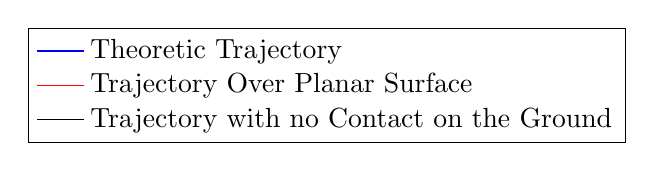
\begin{tikzpicture}
    \begin{customlegend}[legend entries={Theoretic Trajectory,Trajectory Over Planar Surface,Trajectory with no Contact on the Ground},legend cell align=left]
    \addlegendimage{blue,fill=blue,sharp plot}
    \addlegendimage{red,fill=red,sharp plot}
    \addlegendimage{black,fill=black,sharp plot}
    \end{customlegend}
\end{tikzpicture}
\caption{Trajectories of the mobile robot, for both theoretic and experimental cases}
\label{fig:tray}
\end{figure}

The other issues found on this preliminary testing is that the speed measurement by the encoders shows not only verification of the wheel's speed at any given time, but also the wheel's position and distance to the sensor.
In this last case, as can be seen in figure \ref{fig:encoders_temporales}, the amplitude of the maximums is not constant.
This seems to imply that the wheel is loose enough that it moves farther and closer to the sensor and this, in fact, adds more error in this system's trajectory.
These errors are even higher when the robot is on the floor, instead of being suspended. 

\begin{figure}[h]
\centering
\noindent\resizebox{0.95\columnwidth}{!}{
% This file was created by matlab2tikz.
%
%The latest updates can be retrieved from
%  http://www.mathworks.com/matlabcentral/fileexchange/22022-matlab2tikz-matlab2tikz
%where you can also make suggestions and rate matlab2tikz.
%
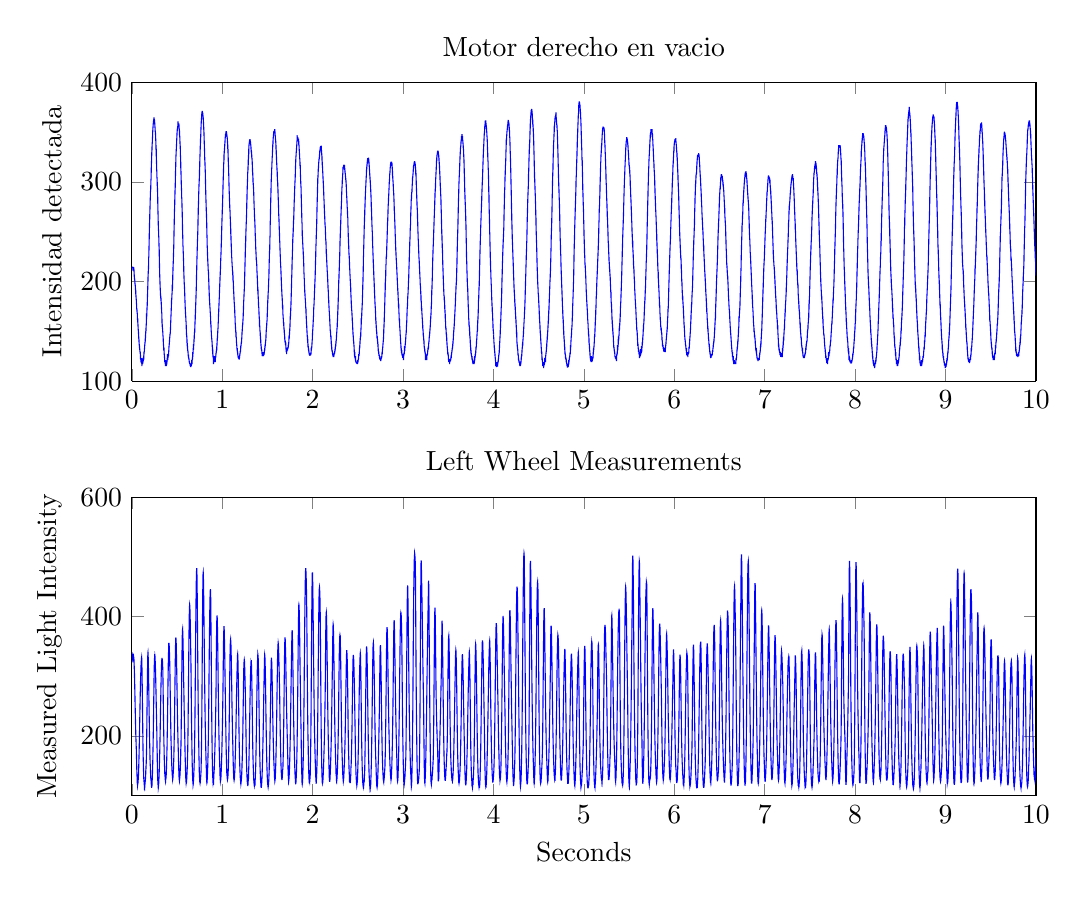
\begin{tikzpicture}

\begin{axis}[%
width=4.521in,
height=1.493in,
at={(0.758in,0.481in)},
scale only axis,
separate axis lines,
every outer x axis line/.append style={black},
every x tick label/.append style={font=\color{black}},
xmin=0,
xmax=10,
xlabel={Seconds},
every outer y axis line/.append style={black},
every y tick label/.append style={font=\color{black}},
ymin=100,
ymax=600,
ylabel={Measured Light Intensity},
axis background/.style={fill=white},
title={Left Wheel Measurements}
]
\addplot [color=blue,solid,forget plot]
  table[row sep=crcr]{%
0.001	331\\
0.002	332\\
0.003	332\\
0.004	329\\
0.005	332\\
0.006	331\\
0.007	332\\
0.008	330\\
0.009	331\\
0.01	335\\
0.011	332\\
0.012	332\\
0.013	328\\
0.014	332\\
0.015	332\\
0.016	331\\
0.017	332\\
0.018	331\\
0.019	331\\
0.02	331\\
0.021	332\\
0.022	331\\
0.023	330\\
0.024	328\\
0.025	323\\
0.026	320\\
0.027	316\\
0.028	311\\
0.029	307\\
0.03	302\\
0.031	294\\
0.032	288\\
0.033	281\\
0.034	273\\
0.035	267\\
0.036	258\\
0.037	251\\
0.038	245\\
0.039	237\\
0.04	231\\
0.041	224\\
0.042	217\\
0.043	212\\
0.044	204\\
0.045	200\\
0.046	195\\
0.047	191\\
0.048	186\\
0.049	182\\
0.05	178\\
0.051	174\\
0.052	166\\
0.053	159\\
0.054	152\\
0.055	145\\
0.056	142\\
0.057	136\\
0.058	133\\
0.059	130\\
0.06	125\\
0.061	121\\
0.062	120\\
0.063	120\\
0.064	117\\
0.065	118\\
0.066	121\\
0.067	119\\
0.068	121\\
0.069	122\\
0.07	124\\
0.071	127\\
0.072	128\\
0.073	131\\
0.074	135\\
0.075	140\\
0.076	144\\
0.077	149\\
0.078	155\\
0.079	160\\
0.08	166\\
0.081	172\\
0.082	179\\
0.083	186\\
0.084	194\\
0.085	201\\
0.086	210\\
0.087	218\\
0.088	227\\
0.089	234\\
0.09	242\\
0.091	251\\
0.092	258\\
0.093	266\\
0.094	273\\
0.095	279\\
0.096	286\\
0.097	292\\
0.098	298\\
0.099	303\\
0.1	307\\
0.101	312\\
0.102	317\\
0.103	320\\
0.104	321\\
0.105	325\\
0.106	327\\
0.107	330\\
0.108	331\\
0.109	332\\
0.11	330\\
0.111	324\\
0.112	317\\
0.113	310\\
0.114	298\\
0.115	289\\
0.116	277\\
0.117	264\\
0.118	254\\
0.119	240\\
0.12	228\\
0.121	218\\
0.122	202\\
0.123	192\\
0.124	181\\
0.125	171\\
0.126	165\\
0.127	160\\
0.128	152\\
0.129	146\\
0.13	141\\
0.131	136\\
0.132	129\\
0.133	129\\
0.134	127\\
0.135	125\\
0.136	122\\
0.137	120\\
0.138	119\\
0.139	116\\
0.14	117\\
0.141	116\\
0.142	117\\
0.143	117\\
0.144	116\\
0.145	118\\
0.146	120\\
0.147	122\\
0.148	123\\
0.149	125\\
0.15	127\\
0.151	128\\
0.152	131\\
0.153	135\\
0.154	136\\
0.155	142\\
0.156	143\\
0.157	146\\
0.158	151\\
0.159	152\\
0.16	157\\
0.161	162\\
0.162	167\\
0.163	176\\
0.164	185\\
0.165	199\\
0.166	211\\
0.167	223\\
0.168	240\\
0.169	250\\
0.17	263\\
0.171	277\\
0.172	287\\
0.173	297\\
0.174	310\\
0.175	318\\
0.176	328\\
0.177	334\\
0.178	339\\
0.179	340\\
0.18	338\\
0.181	335\\
0.182	329\\
0.183	323\\
0.184	315\\
0.185	309\\
0.186	298\\
0.187	288\\
0.188	278\\
0.189	268\\
0.19	257\\
0.191	249\\
0.192	239\\
0.193	228\\
0.194	220\\
0.195	211\\
0.196	202\\
0.197	195\\
0.198	188\\
0.199	181\\
0.2	174\\
0.201	167\\
0.202	160\\
0.203	157\\
0.204	151\\
0.205	149\\
0.206	144\\
0.207	140\\
0.208	135\\
0.209	134\\
0.21	130\\
0.211	130\\
0.212	126\\
0.213	126\\
0.214	123\\
0.215	120\\
0.216	119\\
0.217	119\\
0.218	116\\
0.219	114\\
0.22	114\\
0.221	115\\
0.222	116\\
0.223	117\\
0.224	119\\
0.225	124\\
0.226	127\\
0.227	130\\
0.228	135\\
0.229	139\\
0.23	146\\
0.231	151\\
0.232	157\\
0.233	163\\
0.234	173\\
0.235	180\\
0.236	188\\
0.237	198\\
0.238	207\\
0.239	218\\
0.24	227\\
0.241	239\\
0.242	249\\
0.243	262\\
0.244	271\\
0.245	280\\
0.246	294\\
0.247	305\\
0.248	313\\
0.249	319\\
0.25	324\\
0.251	328\\
0.252	331\\
0.253	334\\
0.254	337\\
0.255	332\\
0.256	334\\
0.257	333\\
0.258	330\\
0.259	325\\
0.26	322\\
0.261	316\\
0.262	311\\
0.263	306\\
0.264	301\\
0.265	293\\
0.266	286\\
0.267	280\\
0.268	273\\
0.269	264\\
0.27	257\\
0.271	248\\
0.272	240\\
0.273	235\\
0.274	228\\
0.275	219\\
0.276	213\\
0.277	206\\
0.278	195\\
0.279	184\\
0.28	174\\
0.281	171\\
0.282	158\\
0.283	150\\
0.284	143\\
0.285	137\\
0.286	133\\
0.287	127\\
0.288	124\\
0.289	121\\
0.29	118\\
0.291	123\\
0.292	116\\
0.293	113\\
0.294	114\\
0.295	116\\
0.296	118\\
0.297	119\\
0.298	121\\
0.299	125\\
0.3	128\\
0.301	130\\
0.302	133\\
0.303	139\\
0.304	143\\
0.305	149\\
0.306	155\\
0.307	158\\
0.308	165\\
0.309	172\\
0.31	178\\
0.311	187\\
0.312	193\\
0.313	201\\
0.314	209\\
0.315	218\\
0.316	227\\
0.317	235\\
0.318	245\\
0.319	253\\
0.32	260\\
0.321	269\\
0.322	277\\
0.323	286\\
0.324	291\\
0.325	298\\
0.326	304\\
0.327	310\\
0.328	315\\
0.329	319\\
0.33	323\\
0.331	325\\
0.332	328\\
0.333	329\\
0.334	330\\
0.335	330\\
0.336	328\\
0.337	328\\
0.338	327\\
0.339	325\\
0.34	323\\
0.341	320\\
0.342	315\\
0.343	311\\
0.344	302\\
0.345	294\\
0.346	284\\
0.347	273\\
0.348	262\\
0.349	248\\
0.35	238\\
0.351	228\\
0.352	218\\
0.353	210\\
0.354	200\\
0.355	191\\
0.356	183\\
0.357	183\\
0.358	171\\
0.359	164\\
0.36	157\\
0.361	155\\
0.362	150\\
0.363	147\\
0.364	142\\
0.365	137\\
0.366	135\\
0.367	133\\
0.368	132\\
0.369	129\\
0.37	128\\
0.371	126\\
0.372	125\\
0.373	126\\
0.374	125\\
0.375	127\\
0.376	128\\
0.377	129\\
0.378	130\\
0.379	130\\
0.38	134\\
0.381	135\\
0.382	141\\
0.383	143\\
0.384	148\\
0.385	152\\
0.386	158\\
0.387	164\\
0.388	169\\
0.389	177\\
0.39	182\\
0.391	191\\
0.392	201\\
0.393	209\\
0.394	218\\
0.395	229\\
0.396	240\\
0.397	250\\
0.398	261\\
0.399	272\\
0.4	284\\
0.401	295\\
0.402	306\\
0.403	311\\
0.404	324\\
0.405	332\\
0.406	338\\
0.407	341\\
0.408	350\\
0.409	355\\
0.41	355\\
0.411	355\\
0.412	355\\
0.413	353\\
0.414	350\\
0.415	348\\
0.416	345\\
0.417	335\\
0.418	333\\
0.419	327\\
0.42	320\\
0.421	312\\
0.422	304\\
0.423	294\\
0.424	283\\
0.425	274\\
0.426	263\\
0.427	253\\
0.428	243\\
0.429	233\\
0.43	226\\
0.431	216\\
0.432	208\\
0.433	201\\
0.434	193\\
0.435	188\\
0.436	182\\
0.437	177\\
0.438	171\\
0.439	167\\
0.44	160\\
0.441	156\\
0.442	153\\
0.443	147\\
0.444	143\\
0.445	142\\
0.446	138\\
0.447	135\\
0.448	134\\
0.449	133\\
0.45	130\\
0.451	129\\
0.452	127\\
0.453	128\\
0.454	128\\
0.455	130\\
0.456	131\\
0.457	133\\
0.458	137\\
0.459	139\\
0.46	141\\
0.461	145\\
0.462	149\\
0.463	153\\
0.464	160\\
0.465	164\\
0.466	171\\
0.467	179\\
0.468	186\\
0.469	193\\
0.47	203\\
0.471	213\\
0.472	223\\
0.473	234\\
0.474	244\\
0.475	258\\
0.476	268\\
0.477	281\\
0.478	294\\
0.479	304\\
0.48	315\\
0.481	326\\
0.482	338\\
0.483	345\\
0.484	352\\
0.485	358\\
0.486	363\\
0.487	364\\
0.488	365\\
0.489	361\\
0.49	362\\
0.491	356\\
0.492	353\\
0.493	346\\
0.494	336\\
0.495	330\\
0.496	320\\
0.497	310\\
0.498	301\\
0.499	293\\
0.5	283\\
0.501	273\\
0.502	265\\
0.503	254\\
0.504	245\\
0.505	235\\
0.506	229\\
0.507	220\\
0.508	214\\
0.509	206\\
0.51	199\\
0.511	194\\
0.512	185\\
0.513	182\\
0.514	177\\
0.515	170\\
0.516	164\\
0.517	158\\
0.518	152\\
0.519	151\\
0.52	142\\
0.521	137\\
0.522	134\\
0.523	130\\
0.524	128\\
0.525	127\\
0.526	126\\
0.527	125\\
0.528	127\\
0.529	129\\
0.53	130\\
0.531	130\\
0.532	133\\
0.533	134\\
0.534	137\\
0.535	141\\
0.536	143\\
0.537	148\\
0.538	151\\
0.539	156\\
0.54	160\\
0.541	167\\
0.542	177\\
0.543	177\\
0.544	185\\
0.545	194\\
0.546	206\\
0.547	218\\
0.548	234\\
0.549	247\\
0.55	262\\
0.551	278\\
0.552	291\\
0.553	305\\
0.554	320\\
0.555	330\\
0.556	345\\
0.557	355\\
0.558	364\\
0.559	371\\
0.56	376\\
0.561	378\\
0.562	379\\
0.563	376\\
0.564	373\\
0.565	369\\
0.566	362\\
0.567	355\\
0.568	347\\
0.569	339\\
0.57	331\\
0.571	320\\
0.572	311\\
0.573	302\\
0.574	291\\
0.575	283\\
0.576	274\\
0.577	267\\
0.578	257\\
0.579	247\\
0.58	240\\
0.581	231\\
0.582	223\\
0.583	218\\
0.584	208\\
0.585	208\\
0.586	198\\
0.587	190\\
0.588	183\\
0.589	174\\
0.59	168\\
0.591	162\\
0.592	156\\
0.593	150\\
0.594	144\\
0.595	140\\
0.596	134\\
0.597	130\\
0.598	127\\
0.599	125\\
0.6	123\\
0.601	121\\
0.602	122\\
0.603	121\\
0.604	121\\
0.605	123\\
0.606	124\\
0.607	127\\
0.608	128\\
0.609	131\\
0.61	135\\
0.611	138\\
0.612	142\\
0.613	145\\
0.614	151\\
0.615	156\\
0.616	161\\
0.617	167\\
0.618	169\\
0.619	181\\
0.62	189\\
0.621	199\\
0.622	209\\
0.623	223\\
0.624	239\\
0.625	255\\
0.626	272\\
0.627	288\\
0.628	303\\
0.629	320\\
0.63	333\\
0.631	347\\
0.632	361\\
0.633	374\\
0.634	385\\
0.635	395\\
0.636	404\\
0.637	409\\
0.638	415\\
0.639	418\\
0.64	420\\
0.641	419\\
0.642	418\\
0.643	413\\
0.644	409\\
0.645	402\\
0.646	395\\
0.647	388\\
0.648	380\\
0.649	370\\
0.65	362\\
0.651	352\\
0.652	342\\
0.653	333\\
0.654	325\\
0.655	312\\
0.656	299\\
0.657	283\\
0.658	267\\
0.659	250\\
0.66	237\\
0.661	221\\
0.662	212\\
0.663	200\\
0.664	191\\
0.665	181\\
0.666	171\\
0.667	164\\
0.668	155\\
0.669	150\\
0.67	142\\
0.671	138\\
0.672	134\\
0.673	129\\
0.674	127\\
0.675	124\\
0.676	121\\
0.677	121\\
0.678	118\\
0.679	119\\
0.68	120\\
0.681	125\\
0.682	124\\
0.683	128\\
0.684	129\\
0.685	132\\
0.686	136\\
0.687	140\\
0.688	144\\
0.689	148\\
0.69	154\\
0.691	158\\
0.692	165\\
0.693	171\\
0.694	180\\
0.695	188\\
0.696	199\\
0.697	210\\
0.698	221\\
0.699	238\\
0.7	254\\
0.701	271\\
0.702	289\\
0.703	307\\
0.704	321\\
0.705	343\\
0.706	360\\
0.707	376\\
0.708	392\\
0.709	404\\
0.71	420\\
0.711	433\\
0.712	445\\
0.713	455\\
0.714	464\\
0.715	470\\
0.716	476\\
0.717	478\\
0.718	480\\
0.719	480\\
0.72	476\\
0.721	467\\
0.722	457\\
0.723	444\\
0.724	432\\
0.725	414\\
0.726	396\\
0.727	379\\
0.728	360\\
0.729	341\\
0.73	324\\
0.731	307\\
0.732	289\\
0.733	274\\
0.734	263\\
0.735	243\\
0.736	231\\
0.737	219\\
0.738	209\\
0.739	201\\
0.74	192\\
0.741	182\\
0.742	173\\
0.743	164\\
0.744	159\\
0.745	152\\
0.746	144\\
0.747	137\\
0.748	136\\
0.749	132\\
0.75	128\\
0.751	126\\
0.752	123\\
0.753	125\\
0.754	122\\
0.755	121\\
0.756	122\\
0.757	122\\
0.758	123\\
0.759	126\\
0.76	127\\
0.761	128\\
0.762	132\\
0.763	133\\
0.764	135\\
0.765	139\\
0.766	141\\
0.767	148\\
0.768	157\\
0.769	165\\
0.77	172\\
0.771	184\\
0.772	195\\
0.773	211\\
0.774	225\\
0.775	243\\
0.776	263\\
0.777	284\\
0.778	306\\
0.779	329\\
0.78	352\\
0.781	373\\
0.782	394\\
0.783	410\\
0.784	426\\
0.785	441\\
0.786	453\\
0.787	463\\
0.788	470\\
0.789	473\\
0.79	474\\
0.791	471\\
0.792	467\\
0.793	458\\
0.794	449\\
0.795	438\\
0.796	427\\
0.797	415\\
0.798	401\\
0.799	388\\
0.8	378\\
0.801	359\\
0.802	347\\
0.803	329\\
0.804	317\\
0.805	304\\
0.806	291\\
0.807	276\\
0.808	266\\
0.809	255\\
0.81	244\\
0.811	232\\
0.812	223\\
0.813	215\\
0.814	206\\
0.815	200\\
0.816	192\\
0.817	185\\
0.818	179\\
0.819	172\\
0.82	167\\
0.821	161\\
0.822	156\\
0.823	151\\
0.824	147\\
0.825	140\\
0.826	135\\
0.827	129\\
0.828	125\\
0.829	123\\
0.83	122\\
0.831	123\\
0.832	121\\
0.833	124\\
0.834	127\\
0.835	130\\
0.836	131\\
0.837	137\\
0.838	141\\
0.839	145\\
0.84	149\\
0.841	156\\
0.842	162\\
0.843	167\\
0.844	176\\
0.845	183\\
0.846	189\\
0.847	202\\
0.848	212\\
0.849	225\\
0.85	238\\
0.851	251\\
0.852	266\\
0.853	281\\
0.854	296\\
0.855	312\\
0.856	326\\
0.857	342\\
0.858	355\\
0.859	370\\
0.86	381\\
0.861	392\\
0.862	403\\
0.863	413\\
0.864	422\\
0.865	430\\
0.866	435\\
0.867	440\\
0.868	443\\
0.869	445\\
0.87	445\\
0.871	442\\
0.872	439\\
0.873	429\\
0.874	415\\
0.875	399\\
0.876	380\\
0.877	362\\
0.878	345\\
0.879	326\\
0.88	306\\
0.881	290\\
0.882	272\\
0.883	254\\
0.884	236\\
0.885	223\\
0.886	208\\
0.887	195\\
0.888	186\\
0.889	174\\
0.89	164\\
0.891	157\\
0.892	150\\
0.893	143\\
0.894	137\\
0.895	133\\
0.896	130\\
0.897	125\\
0.898	123\\
0.899	121\\
0.9	122\\
0.901	120\\
0.902	122\\
0.903	118\\
0.904	124\\
0.905	126\\
0.906	128\\
0.907	131\\
0.908	133\\
0.909	139\\
0.91	139\\
0.911	142\\
0.912	145\\
0.913	151\\
0.914	155\\
0.915	160\\
0.916	164\\
0.917	168\\
0.918	172\\
0.919	178\\
0.92	183\\
0.921	189\\
0.922	195\\
0.923	201\\
0.924	209\\
0.925	216\\
0.926	223\\
0.927	230\\
0.928	240\\
0.929	247\\
0.93	256\\
0.931	265\\
0.932	282\\
0.933	301\\
0.934	318\\
0.935	335\\
0.936	349\\
0.937	362\\
0.938	375\\
0.939	385\\
0.94	392\\
0.941	396\\
0.942	400\\
0.943	401\\
0.944	401\\
0.945	396\\
0.946	392\\
0.947	385\\
0.948	378\\
0.949	368\\
0.95	357\\
0.951	346\\
0.952	333\\
0.953	322\\
0.954	311\\
0.955	296\\
0.956	283\\
0.957	272\\
0.958	260\\
0.959	248\\
0.96	236\\
0.961	228\\
0.962	221\\
0.963	208\\
0.964	201\\
0.965	194\\
0.966	186\\
0.967	179\\
0.968	174\\
0.969	169\\
0.97	164\\
0.971	157\\
0.972	154\\
0.973	150\\
0.974	145\\
0.975	139\\
0.976	134\\
0.977	130\\
0.978	128\\
0.979	126\\
0.98	124\\
0.981	125\\
0.982	125\\
0.983	125\\
0.984	128\\
0.985	130\\
0.986	131\\
0.987	135\\
0.988	137\\
0.989	141\\
0.99	146\\
0.991	148\\
0.992	154\\
0.993	159\\
0.994	162\\
0.995	168\\
0.996	174\\
0.997	181\\
0.998	188\\
0.999	193\\
1	201\\
1.001	207\\
1.002	215\\
1.003	224\\
1.004	231\\
1.005	242\\
1.006	252\\
1.007	262\\
1.008	272\\
1.009	284\\
1.01	298\\
1.011	311\\
1.012	325\\
1.013	335\\
1.014	348\\
1.015	361\\
1.016	366\\
1.017	372\\
1.018	378\\
1.019	381\\
1.02	383\\
1.021	383\\
1.022	378\\
1.023	372\\
1.024	368\\
1.025	360\\
1.026	353\\
1.027	346\\
1.028	335\\
1.029	326\\
1.03	316\\
1.031	304\\
1.032	294\\
1.033	282\\
1.034	273\\
1.035	261\\
1.036	249\\
1.037	240\\
1.038	230\\
1.039	221\\
1.04	213\\
1.041	203\\
1.042	194\\
1.043	185\\
1.044	178\\
1.045	170\\
1.046	164\\
1.047	160\\
1.048	154\\
1.049	148\\
1.05	143\\
1.051	137\\
1.052	137\\
1.053	134\\
1.054	133\\
1.055	130\\
1.056	129\\
1.057	128\\
1.058	127\\
1.059	128\\
1.06	128\\
1.061	129\\
1.062	131\\
1.063	134\\
1.064	134\\
1.065	137\\
1.066	141\\
1.067	142\\
1.068	150\\
1.069	155\\
1.07	160\\
1.071	168\\
1.072	175\\
1.073	183\\
1.074	190\\
1.075	195\\
1.076	209\\
1.077	220\\
1.078	229\\
1.079	243\\
1.08	255\\
1.081	268\\
1.082	282\\
1.083	296\\
1.084	308\\
1.085	319\\
1.086	330\\
1.087	339\\
1.088	346\\
1.089	352\\
1.09	357\\
1.091	360\\
1.092	361\\
1.093	362\\
1.094	360\\
1.095	359\\
1.096	355\\
1.097	351\\
1.098	346\\
1.099	338\\
1.1	331\\
1.101	323\\
1.102	314\\
1.103	305\\
1.104	294\\
1.105	285\\
1.106	276\\
1.107	266\\
1.108	254\\
1.109	246\\
1.11	238\\
1.111	230\\
1.112	220\\
1.113	213\\
1.114	206\\
1.115	200\\
1.116	193\\
1.117	187\\
1.118	181\\
1.119	173\\
1.12	166\\
1.121	160\\
1.122	153\\
1.123	148\\
1.124	143\\
1.125	139\\
1.126	136\\
1.127	131\\
1.128	129\\
1.129	128\\
1.13	127\\
1.131	126\\
1.132	127\\
1.133	129\\
1.134	128\\
1.135	129\\
1.136	132\\
1.137	136\\
1.138	138\\
1.139	140\\
1.14	144\\
1.141	146\\
1.142	154\\
1.143	158\\
1.144	162\\
1.145	168\\
1.146	174\\
1.147	177\\
1.148	188\\
1.149	194\\
1.15	200\\
1.151	202\\
1.152	213\\
1.153	222\\
1.154	231\\
1.155	239\\
1.156	246\\
1.157	254\\
1.158	263\\
1.159	273\\
1.16	279\\
1.161	287\\
1.162	293\\
1.163	300\\
1.164	307\\
1.165	312\\
1.166	318\\
1.167	323\\
1.168	328\\
1.169	334\\
1.17	336\\
1.171	337\\
1.172	335\\
1.173	332\\
1.174	327\\
1.175	321\\
1.176	314\\
1.177	304\\
1.178	296\\
1.179	285\\
1.18	273\\
1.181	264\\
1.182	251\\
1.183	240\\
1.184	229\\
1.185	216\\
1.186	207\\
1.187	197\\
1.188	189\\
1.189	181\\
1.19	171\\
1.191	167\\
1.192	161\\
1.193	157\\
1.194	152\\
1.195	147\\
1.196	144\\
1.197	140\\
1.198	136\\
1.199	134\\
1.2	130\\
1.201	128\\
1.202	127\\
1.203	125\\
1.204	120\\
1.205	122\\
1.206	122\\
1.207	120\\
1.208	121\\
1.209	123\\
1.21	124\\
1.211	125\\
1.212	129\\
1.213	129\\
1.214	130\\
1.215	135\\
1.216	136\\
1.217	142\\
1.218	145\\
1.219	149\\
1.22	159\\
1.221	158\\
1.222	165\\
1.223	169\\
1.224	177\\
1.225	184\\
1.226	191\\
1.227	197\\
1.228	206\\
1.229	216\\
1.23	227\\
1.231	237\\
1.232	249\\
1.233	257\\
1.234	270\\
1.235	280\\
1.236	291\\
1.237	300\\
1.238	307\\
1.239	315\\
1.24	320\\
1.241	323\\
1.242	324\\
1.243	327\\
1.244	328\\
1.245	327\\
1.246	325\\
1.247	318\\
1.248	317\\
1.249	314\\
1.25	307\\
1.251	303\\
1.252	297\\
1.253	291\\
1.254	284\\
1.255	277\\
1.256	268\\
1.257	260\\
1.258	251\\
1.259	243\\
1.26	236\\
1.261	227\\
1.262	218\\
1.263	206\\
1.264	195\\
1.265	185\\
1.266	173\\
1.267	169\\
1.268	161\\
1.269	156\\
1.27	149\\
1.271	146\\
1.272	140\\
1.273	141\\
1.274	133\\
1.275	130\\
1.276	125\\
1.277	125\\
1.278	122\\
1.279	122\\
1.28	120\\
1.281	119\\
1.282	119\\
1.283	117\\
1.284	117\\
1.285	119\\
1.286	121\\
1.287	123\\
1.288	126\\
1.289	128\\
1.29	127\\
1.291	134\\
1.292	139\\
1.293	144\\
1.294	148\\
1.295	155\\
1.296	160\\
1.297	167\\
1.298	175\\
1.299	182\\
1.3	190\\
1.301	200\\
1.302	210\\
1.303	218\\
1.304	227\\
1.305	237\\
1.306	245\\
1.307	254\\
1.308	264\\
1.309	271\\
1.31	279\\
1.311	287\\
1.312	296\\
1.313	300\\
1.314	306\\
1.315	312\\
1.316	316\\
1.317	319\\
1.318	322\\
1.319	321\\
1.32	324\\
1.321	326\\
1.322	326\\
1.323	322\\
1.324	316\\
1.325	311\\
1.326	304\\
1.327	295\\
1.328	285\\
1.329	278\\
1.33	268\\
1.331	257\\
1.332	244\\
1.333	233\\
1.334	222\\
1.335	210\\
1.336	201\\
1.337	192\\
1.338	180\\
1.339	175\\
1.34	167\\
1.341	161\\
1.342	157\\
1.343	150\\
1.344	146\\
1.345	141\\
1.346	137\\
1.347	134\\
1.348	130\\
1.349	127\\
1.35	124\\
1.351	123\\
1.352	121\\
1.353	119\\
1.354	118\\
1.355	120\\
1.356	115\\
1.357	117\\
1.358	117\\
1.359	121\\
1.36	118\\
1.361	118\\
1.362	117\\
1.363	122\\
1.364	124\\
1.365	128\\
1.366	127\\
1.367	134\\
1.368	138\\
1.369	141\\
1.37	146\\
1.371	152\\
1.372	158\\
1.373	166\\
1.374	174\\
1.375	181\\
1.376	190\\
1.377	200\\
1.378	211\\
1.379	220\\
1.38	232\\
1.381	243\\
1.382	252\\
1.383	263\\
1.384	274\\
1.385	282\\
1.386	293\\
1.387	301\\
1.388	310\\
1.389	317\\
1.39	322\\
1.391	327\\
1.392	332\\
1.393	334\\
1.394	337\\
1.395	336\\
1.396	334\\
1.397	332\\
1.398	330\\
1.399	324\\
1.4	317\\
1.401	312\\
1.402	305\\
1.403	295\\
1.404	286\\
1.405	275\\
1.406	264\\
1.407	252\\
1.408	242\\
1.409	229\\
1.41	219\\
1.411	207\\
1.412	196\\
1.413	187\\
1.414	178\\
1.415	171\\
1.416	164\\
1.417	159\\
1.418	151\\
1.419	145\\
1.42	142\\
1.421	138\\
1.422	133\\
1.423	130\\
1.424	126\\
1.425	129\\
1.426	122\\
1.427	121\\
1.428	118\\
1.429	116\\
1.43	114\\
1.431	114\\
1.432	114\\
1.433	115\\
1.434	116\\
1.435	118\\
1.436	119\\
1.437	122\\
1.438	123\\
1.439	128\\
1.44	129\\
1.441	135\\
1.442	138\\
1.443	143\\
1.444	148\\
1.445	154\\
1.446	160\\
1.447	164\\
1.448	172\\
1.449	178\\
1.45	185\\
1.451	192\\
1.452	200\\
1.453	207\\
1.454	217\\
1.455	225\\
1.456	233\\
1.457	242\\
1.458	253\\
1.459	261\\
1.46	270\\
1.461	278\\
1.462	283\\
1.463	294\\
1.464	301\\
1.465	308\\
1.466	316\\
1.467	324\\
1.468	330\\
1.469	333\\
1.47	336\\
1.471	335\\
1.472	333\\
1.473	330\\
1.474	325\\
1.475	319\\
1.476	314\\
1.477	305\\
1.478	298\\
1.479	290\\
1.48	280\\
1.481	268\\
1.482	256\\
1.483	245\\
1.484	234\\
1.485	222\\
1.486	214\\
1.487	205\\
1.488	194\\
1.489	185\\
1.49	177\\
1.491	171\\
1.492	165\\
1.493	157\\
1.494	151\\
1.495	147\\
1.496	142\\
1.497	138\\
1.498	133\\
1.499	130\\
1.5	128\\
1.501	123\\
1.502	122\\
1.503	118\\
1.504	119\\
1.505	118\\
1.506	116\\
1.507	115\\
1.508	114\\
1.509	115\\
1.51	116\\
1.511	121\\
1.512	118\\
1.513	121\\
1.514	123\\
1.515	126\\
1.516	130\\
1.517	133\\
1.518	137\\
1.519	142\\
1.52	144\\
1.521	157\\
1.522	158\\
1.523	162\\
1.524	168\\
1.525	174\\
1.526	182\\
1.527	190\\
1.528	195\\
1.529	206\\
1.53	217\\
1.531	223\\
1.532	232\\
1.533	239\\
1.534	250\\
1.535	260\\
1.536	272\\
1.537	283\\
1.538	293\\
1.539	302\\
1.54	311\\
1.541	318\\
1.542	322\\
1.543	327\\
1.544	331\\
1.545	329\\
1.546	329\\
1.547	327\\
1.548	319\\
1.549	318\\
1.55	312\\
1.551	305\\
1.552	297\\
1.553	290\\
1.554	285\\
1.555	272\\
1.556	262\\
1.557	251\\
1.558	244\\
1.559	235\\
1.56	226\\
1.561	219\\
1.562	209\\
1.563	203\\
1.564	196\\
1.565	189\\
1.566	183\\
1.567	176\\
1.568	173\\
1.569	169\\
1.57	164\\
1.571	157\\
1.572	155\\
1.573	152\\
1.574	147\\
1.575	144\\
1.576	142\\
1.577	137\\
1.578	134\\
1.579	130\\
1.58	128\\
1.581	127\\
1.582	125\\
1.583	126\\
1.584	128\\
1.585	127\\
1.586	128\\
1.587	129\\
1.588	135\\
1.589	138\\
1.59	143\\
1.591	146\\
1.592	152\\
1.593	155\\
1.594	162\\
1.595	168\\
1.596	175\\
1.597	182\\
1.598	189\\
1.599	197\\
1.6	205\\
1.601	215\\
1.602	224\\
1.603	235\\
1.604	246\\
1.605	257\\
1.606	267\\
1.607	278\\
1.608	288\\
1.609	300\\
1.61	307\\
1.611	319\\
1.612	329\\
1.613	335\\
1.614	342\\
1.615	345\\
1.616	351\\
1.617	353\\
1.618	354\\
1.619	356\\
1.62	355\\
1.621	352\\
1.622	350\\
1.623	346\\
1.624	343\\
1.625	337\\
1.626	333\\
1.627	327\\
1.628	320\\
1.629	314\\
1.63	309\\
1.631	302\\
1.632	294\\
1.633	288\\
1.634	282\\
1.635	274\\
1.636	265\\
1.637	253\\
1.638	243\\
1.639	232\\
1.64	223\\
1.641	214\\
1.642	204\\
1.643	195\\
1.644	189\\
1.645	180\\
1.646	178\\
1.647	168\\
1.648	165\\
1.649	159\\
1.65	152\\
1.651	149\\
1.652	145\\
1.653	140\\
1.654	138\\
1.655	134\\
1.656	133\\
1.657	130\\
1.658	129\\
1.659	128\\
1.66	127\\
1.661	127\\
1.662	128\\
1.663	128\\
1.664	131\\
1.665	133\\
1.666	135\\
1.667	139\\
1.668	140\\
1.669	144\\
1.67	144\\
1.671	148\\
1.672	149\\
1.673	157\\
1.674	161\\
1.675	168\\
1.676	175\\
1.677	184\\
1.678	194\\
1.679	202\\
1.68	214\\
1.681	225\\
1.682	239\\
1.683	252\\
1.684	265\\
1.685	279\\
1.686	292\\
1.687	306\\
1.688	319\\
1.689	330\\
1.69	340\\
1.691	350\\
1.692	356\\
1.693	360\\
1.694	364\\
1.695	364\\
1.696	363\\
1.697	361\\
1.698	357\\
1.699	352\\
1.7	343\\
1.701	338\\
1.702	333\\
1.703	325\\
1.704	314\\
1.705	307\\
1.706	297\\
1.707	287\\
1.708	280\\
1.709	272\\
1.71	263\\
1.711	255\\
1.712	248\\
1.713	240\\
1.714	231\\
1.715	225\\
1.716	220\\
1.717	213\\
1.718	207\\
1.719	201\\
1.72	196\\
1.721	191\\
1.722	184\\
1.723	176\\
1.724	170\\
1.725	164\\
1.726	158\\
1.727	151\\
1.728	146\\
1.729	137\\
1.73	137\\
1.731	133\\
1.732	131\\
1.733	128\\
1.734	125\\
1.735	126\\
1.736	125\\
1.737	126\\
1.738	128\\
1.739	130\\
1.74	132\\
1.741	135\\
1.742	138\\
1.743	142\\
1.744	146\\
1.745	152\\
1.746	156\\
1.747	159\\
1.748	167\\
1.749	173\\
1.75	179\\
1.751	186\\
1.752	194\\
1.753	202\\
1.754	212\\
1.755	220\\
1.756	228\\
1.757	240\\
1.758	251\\
1.759	258\\
1.76	269\\
1.761	281\\
1.762	287\\
1.763	299\\
1.764	310\\
1.765	321\\
1.766	328\\
1.767	336\\
1.768	344\\
1.769	354\\
1.77	362\\
1.771	371\\
1.772	373\\
1.773	377\\
1.774	376\\
1.775	375\\
1.776	368\\
1.777	361\\
1.778	354\\
1.779	345\\
1.78	335\\
1.781	327\\
1.782	314\\
1.783	304\\
1.784	293\\
1.785	283\\
1.786	272\\
1.787	260\\
1.788	251\\
1.789	239\\
1.79	230\\
1.791	222\\
1.792	213\\
1.793	204\\
1.794	198\\
1.795	189\\
1.796	183\\
1.797	177\\
1.798	172\\
1.799	165\\
1.8	160\\
1.801	155\\
1.802	152\\
1.803	146\\
1.804	143\\
1.805	137\\
1.806	135\\
1.807	131\\
1.808	130\\
1.809	126\\
1.81	123\\
1.811	122\\
1.812	120\\
1.813	120\\
1.814	121\\
1.815	122\\
1.816	123\\
1.817	125\\
1.818	129\\
1.819	131\\
1.82	135\\
1.821	139\\
1.822	143\\
1.823	148\\
1.824	155\\
1.825	160\\
1.826	168\\
1.827	177\\
1.828	184\\
1.829	196\\
1.83	204\\
1.831	217\\
1.832	226\\
1.833	239\\
1.834	254\\
1.835	267\\
1.836	282\\
1.837	299\\
1.838	314\\
1.839	331\\
1.84	347\\
1.841	360\\
1.842	375\\
1.843	388\\
1.844	396\\
1.845	406\\
1.846	413\\
1.847	419\\
1.848	420\\
1.849	419\\
1.85	418\\
1.851	413\\
1.852	408\\
1.853	401\\
1.854	392\\
1.855	383\\
1.856	374\\
1.857	364\\
1.858	352\\
1.859	340\\
1.86	329\\
1.861	318\\
1.862	307\\
1.863	296\\
1.864	284\\
1.865	273\\
1.866	264\\
1.867	253\\
1.868	244\\
1.869	235\\
1.87	226\\
1.871	219\\
1.872	212\\
1.873	199\\
1.874	189\\
1.875	176\\
1.876	168\\
1.877	157\\
1.878	150\\
1.879	144\\
1.88	138\\
1.881	130\\
1.882	122\\
1.883	124\\
1.884	120\\
1.885	119\\
1.886	120\\
1.887	119\\
1.888	125\\
1.889	124\\
1.89	128\\
1.891	132\\
1.892	136\\
1.893	143\\
1.894	146\\
1.895	152\\
1.896	161\\
1.897	165\\
1.898	176\\
1.899	185\\
1.9	195\\
1.901	206\\
1.902	218\\
1.903	231\\
1.904	248\\
1.905	260\\
1.906	279\\
1.907	297\\
1.908	317\\
1.909	331\\
1.91	345\\
1.911	360\\
1.912	378\\
1.913	393\\
1.914	407\\
1.915	419\\
1.916	430\\
1.917	442\\
1.918	452\\
1.919	461\\
1.92	469\\
1.921	474\\
1.922	478\\
1.923	479\\
1.924	481\\
1.925	476\\
1.926	476\\
1.927	472\\
1.928	469\\
1.929	463\\
1.93	455\\
1.931	450\\
1.932	443\\
1.933	435\\
1.934	424\\
1.935	406\\
1.936	393\\
1.937	375\\
1.938	356\\
1.939	336\\
1.94	318\\
1.941	300\\
1.942	284\\
1.943	269\\
1.944	253\\
1.945	241\\
1.946	227\\
1.947	215\\
1.948	205\\
1.949	195\\
1.95	187\\
1.951	183\\
1.952	170\\
1.953	162\\
1.954	153\\
1.955	150\\
1.956	145\\
1.957	141\\
1.958	135\\
1.959	131\\
1.96	129\\
1.961	125\\
1.962	124\\
1.963	122\\
1.964	121\\
1.965	121\\
1.966	121\\
1.967	125\\
1.968	124\\
1.969	126\\
1.97	128\\
1.971	129\\
1.972	132\\
1.973	133\\
1.974	141\\
1.975	148\\
1.976	157\\
1.977	165\\
1.978	174\\
1.979	186\\
1.98	197\\
1.981	211\\
1.982	227\\
1.983	246\\
1.984	271\\
1.985	289\\
1.986	311\\
1.987	334\\
1.988	356\\
1.989	376\\
1.99	396\\
1.991	414\\
1.992	430\\
1.993	443\\
1.994	455\\
1.995	465\\
1.996	473\\
1.997	472\\
1.998	474\\
1.999	470\\
2	464\\
2.001	456\\
2.002	445\\
2.003	436\\
2.004	425\\
2.005	411\\
2.006	397\\
2.007	383\\
2.008	369\\
2.009	355\\
2.01	340\\
2.011	323\\
2.012	312\\
2.013	301\\
2.014	285\\
2.015	272\\
2.016	261\\
2.017	248\\
2.018	237\\
2.019	229\\
2.02	218\\
2.021	206\\
2.022	202\\
2.023	195\\
2.024	188\\
2.025	181\\
2.026	176\\
2.027	169\\
2.028	163\\
2.029	158\\
2.03	152\\
2.031	148\\
2.032	144\\
2.033	139\\
2.034	136\\
2.035	131\\
2.036	127\\
2.037	129\\
2.038	123\\
2.039	120\\
2.04	123\\
2.041	124\\
2.042	128\\
2.043	130\\
2.044	131\\
2.045	137\\
2.046	142\\
2.047	146\\
2.048	151\\
2.049	159\\
2.05	164\\
2.051	171\\
2.052	179\\
2.053	188\\
2.054	195\\
2.055	211\\
2.056	223\\
2.057	235\\
2.058	250\\
2.059	266\\
2.06	282\\
2.061	299\\
2.062	316\\
2.063	333\\
2.064	345\\
2.065	363\\
2.066	378\\
2.067	390\\
2.068	404\\
2.069	414\\
2.07	424\\
2.071	433\\
2.072	440\\
2.073	444\\
2.074	447\\
2.075	448\\
2.076	449\\
2.077	447\\
2.078	444\\
2.079	441\\
2.08	436\\
2.081	431\\
2.082	422\\
2.083	415\\
2.084	404\\
2.085	388\\
2.086	371\\
2.087	353\\
2.088	331\\
2.089	313\\
2.09	293\\
2.091	272\\
2.092	255\\
2.093	236\\
2.094	223\\
2.095	208\\
2.096	195\\
2.097	185\\
2.098	174\\
2.099	164\\
2.1	156\\
2.101	148\\
2.102	143\\
2.103	136\\
2.104	132\\
2.105	127\\
2.106	125\\
2.107	122\\
2.108	121\\
2.109	122\\
2.11	121\\
2.111	121\\
2.112	123\\
2.113	124\\
2.114	126\\
2.115	130\\
2.116	132\\
2.117	135\\
2.118	138\\
2.119	142\\
2.12	145\\
2.121	149\\
2.122	155\\
2.123	158\\
2.124	164\\
2.125	169\\
2.126	174\\
2.127	178\\
2.128	185\\
2.129	190\\
2.13	194\\
2.131	204\\
2.132	213\\
2.133	219\\
2.134	227\\
2.135	233\\
2.136	243\\
2.137	253\\
2.138	264\\
2.139	274\\
2.14	287\\
2.141	304\\
2.142	323\\
2.143	340\\
2.144	354\\
2.145	369\\
2.146	381\\
2.147	390\\
2.148	398\\
2.149	404\\
2.15	406\\
2.151	407\\
2.152	404\\
2.153	402\\
2.154	396\\
2.155	390\\
2.156	382\\
2.157	371\\
2.158	363\\
2.159	350\\
2.16	339\\
2.161	326\\
2.162	314\\
2.163	300\\
2.164	289\\
2.165	279\\
2.166	265\\
2.167	253\\
2.168	242\\
2.169	231\\
2.17	221\\
2.171	213\\
2.172	204\\
2.173	195\\
2.174	190\\
2.175	181\\
2.176	175\\
2.177	171\\
2.178	166\\
2.179	160\\
2.18	154\\
2.181	150\\
2.182	142\\
2.183	133\\
2.184	132\\
2.185	128\\
2.186	126\\
2.187	125\\
2.188	124\\
2.189	124\\
2.19	125\\
2.191	128\\
2.192	128\\
2.193	131\\
2.194	135\\
2.195	136\\
2.196	140\\
2.197	145\\
2.198	149\\
2.199	157\\
2.2	159\\
2.201	164\\
2.202	171\\
2.203	176\\
2.204	181\\
2.205	187\\
2.206	196\\
2.207	201\\
2.208	211\\
2.209	220\\
2.21	228\\
2.211	237\\
2.212	248\\
2.213	258\\
2.214	269\\
2.215	281\\
2.216	290\\
2.217	300\\
2.218	313\\
2.219	320\\
2.22	330\\
2.221	340\\
2.222	354\\
2.223	366\\
2.224	375\\
2.225	382\\
2.226	385\\
2.227	387\\
2.228	386\\
2.229	383\\
2.23	378\\
2.231	370\\
2.232	367\\
2.233	354\\
2.234	344\\
2.235	333\\
2.236	323\\
2.237	309\\
2.238	300\\
2.239	287\\
2.24	275\\
2.241	263\\
2.242	257\\
2.243	242\\
2.244	232\\
2.245	221\\
2.246	213\\
2.247	205\\
2.248	198\\
2.249	191\\
2.25	183\\
2.251	179\\
2.252	173\\
2.253	166\\
2.254	162\\
2.255	156\\
2.256	153\\
2.257	150\\
2.258	145\\
2.259	137\\
2.26	137\\
2.261	137\\
2.262	132\\
2.263	129\\
2.264	130\\
2.265	128\\
2.266	127\\
2.267	126\\
2.268	128\\
2.269	129\\
2.27	129\\
2.271	133\\
2.272	136\\
2.273	140\\
2.274	143\\
2.275	147\\
2.276	153\\
2.277	158\\
2.278	166\\
2.279	172\\
2.28	178\\
2.281	186\\
2.282	195\\
2.283	201\\
2.284	212\\
2.285	223\\
2.286	231\\
2.287	244\\
2.288	256\\
2.289	268\\
2.29	280\\
2.291	293\\
2.292	305\\
2.293	317\\
2.294	328\\
2.295	338\\
2.296	345\\
2.297	353\\
2.298	357\\
2.299	361\\
2.3	366\\
2.301	368\\
2.302	369\\
2.303	368\\
2.304	366\\
2.305	368\\
2.306	361\\
2.307	355\\
2.308	345\\
2.309	341\\
2.31	330\\
2.311	320\\
2.312	306\\
2.313	295\\
2.314	285\\
2.315	270\\
2.316	256\\
2.317	243\\
2.318	233\\
2.319	222\\
2.32	213\\
2.321	204\\
2.322	191\\
2.323	188\\
2.324	183\\
2.325	174\\
2.326	169\\
2.327	164\\
2.328	160\\
2.329	153\\
2.33	151\\
2.331	146\\
2.332	138\\
2.333	139\\
2.334	133\\
2.335	132\\
2.336	130\\
2.337	127\\
2.338	124\\
2.339	126\\
2.34	124\\
2.341	125\\
2.342	127\\
2.343	130\\
2.344	130\\
2.345	134\\
2.346	136\\
2.347	139\\
2.348	142\\
2.349	147\\
2.35	150\\
2.351	152\\
2.352	156\\
2.353	162\\
2.354	166\\
2.355	173\\
2.356	178\\
2.357	183\\
2.358	188\\
2.359	196\\
2.36	203\\
2.361	213\\
2.362	220\\
2.363	231\\
2.364	238\\
2.365	248\\
2.366	258\\
2.367	267\\
2.368	277\\
2.369	287\\
2.37	298\\
2.371	311\\
2.372	317\\
2.373	324\\
2.374	331\\
2.375	337\\
2.376	340\\
2.377	343\\
2.378	343\\
2.379	341\\
2.38	337\\
2.381	334\\
2.382	330\\
2.383	326\\
2.384	317\\
2.385	309\\
2.386	300\\
2.387	290\\
2.388	278\\
2.389	265\\
2.39	254\\
2.391	238\\
2.392	226\\
2.393	215\\
2.394	201\\
2.395	194\\
2.396	186\\
2.397	178\\
2.398	169\\
2.399	166\\
2.4	161\\
2.401	154\\
2.402	150\\
2.403	144\\
2.404	142\\
2.405	137\\
2.406	135\\
2.407	132\\
2.408	123\\
2.409	127\\
2.41	124\\
2.411	123\\
2.412	123\\
2.413	122\\
2.414	122\\
2.415	122\\
2.416	122\\
2.417	124\\
2.418	125\\
2.419	128\\
2.42	128\\
2.421	133\\
2.422	135\\
2.423	138\\
2.424	149\\
2.425	147\\
2.426	152\\
2.427	155\\
2.428	162\\
2.429	166\\
2.43	173\\
2.431	179\\
2.432	186\\
2.433	192\\
2.434	201\\
2.435	208\\
2.436	218\\
2.437	230\\
2.438	242\\
2.439	254\\
2.44	268\\
2.441	277\\
2.442	287\\
2.443	298\\
2.444	306\\
2.445	313\\
2.446	322\\
2.447	329\\
2.448	332\\
2.449	334\\
2.45	335\\
2.451	335\\
2.452	333\\
2.453	332\\
2.454	329\\
2.455	326\\
2.456	320\\
2.457	315\\
2.458	310\\
2.459	303\\
2.46	295\\
2.461	288\\
2.462	281\\
2.463	271\\
2.464	262\\
2.465	256\\
2.466	246\\
2.467	238\\
2.468	228\\
2.469	218\\
2.47	208\\
2.471	198\\
2.472	187\\
2.473	178\\
2.474	170\\
2.475	162\\
2.476	156\\
2.477	153\\
2.478	146\\
2.479	140\\
2.48	136\\
2.481	132\\
2.482	129\\
2.483	127\\
2.484	124\\
2.485	121\\
2.486	120\\
2.487	121\\
2.488	119\\
2.489	117\\
2.49	118\\
2.491	119\\
2.492	120\\
2.493	122\\
2.494	123\\
2.495	126\\
2.496	127\\
2.497	133\\
2.498	136\\
2.499	140\\
2.5	147\\
2.501	151\\
2.502	156\\
2.503	163\\
2.504	169\\
2.505	176\\
2.506	183\\
2.507	191\\
2.508	201\\
2.509	212\\
2.51	225\\
2.511	231\\
2.512	241\\
2.513	250\\
2.514	259\\
2.515	268\\
2.516	280\\
2.517	286\\
2.518	294\\
2.519	302\\
2.52	309\\
2.521	315\\
2.522	320\\
2.523	325\\
2.524	329\\
2.525	334\\
2.526	338\\
2.527	339\\
2.528	337\\
2.529	336\\
2.53	329\\
2.531	322\\
2.532	313\\
2.533	306\\
2.534	296\\
2.535	286\\
2.536	272\\
2.537	257\\
2.538	247\\
2.539	233\\
2.54	220\\
2.541	208\\
2.542	198\\
2.543	186\\
2.544	178\\
2.545	169\\
2.546	162\\
2.547	156\\
2.548	149\\
2.549	144\\
2.55	139\\
2.551	135\\
2.552	130\\
2.553	127\\
2.554	126\\
2.555	121\\
2.556	122\\
2.557	118\\
2.558	117\\
2.559	118\\
2.56	116\\
2.561	114\\
2.562	116\\
2.563	117\\
2.564	116\\
2.565	118\\
2.566	117\\
2.567	122\\
2.568	123\\
2.569	124\\
2.57	122\\
2.571	127\\
2.572	133\\
2.573	133\\
2.574	136\\
2.575	139\\
2.576	142\\
2.577	151\\
2.578	160\\
2.579	168\\
2.58	177\\
2.581	187\\
2.582	197\\
2.583	210\\
2.584	223\\
2.585	235\\
2.586	250\\
2.587	264\\
2.588	278\\
2.589	290\\
2.59	304\\
2.591	316\\
2.592	325\\
2.593	333\\
2.594	341\\
2.595	346\\
2.596	348\\
2.597	350\\
2.598	347\\
2.599	347\\
2.6	343\\
2.601	339\\
2.602	333\\
2.603	325\\
2.604	317\\
2.605	309\\
2.606	298\\
2.607	285\\
2.608	276\\
2.609	263\\
2.61	252\\
2.611	241\\
2.612	228\\
2.613	218\\
2.614	207\\
2.615	199\\
2.616	189\\
2.617	180\\
2.618	174\\
2.619	164\\
2.62	159\\
2.621	154\\
2.622	150\\
2.623	144\\
2.624	139\\
2.625	136\\
2.626	132\\
2.627	129\\
2.628	127\\
2.629	124\\
2.63	122\\
2.631	122\\
2.632	117\\
2.633	117\\
2.634	114\\
2.635	115\\
2.636	114\\
2.637	113\\
2.638	115\\
2.639	114\\
2.64	115\\
2.641	115\\
2.642	118\\
2.643	121\\
2.644	125\\
2.645	131\\
2.646	134\\
2.647	140\\
2.648	146\\
2.649	151\\
2.65	160\\
2.651	167\\
2.652	174\\
2.653	184\\
2.654	193\\
2.655	204\\
2.656	212\\
2.657	228\\
2.658	243\\
2.659	252\\
2.66	266\\
2.661	278\\
2.662	290\\
2.663	301\\
2.664	314\\
2.665	323\\
2.666	334\\
2.667	342\\
2.668	348\\
2.669	352\\
2.67	356\\
2.671	355\\
2.672	356\\
2.673	353\\
2.674	350\\
2.675	344\\
2.676	339\\
2.677	332\\
2.678	327\\
2.679	320\\
2.68	312\\
2.681	303\\
2.682	297\\
2.683	284\\
2.684	272\\
2.685	260\\
2.686	253\\
2.687	243\\
2.688	233\\
2.689	224\\
2.69	213\\
2.691	206\\
2.692	201\\
2.693	191\\
2.694	186\\
2.695	179\\
2.696	174\\
2.697	168\\
2.698	163\\
2.699	160\\
2.7	155\\
2.701	151\\
2.702	145\\
2.703	139\\
2.704	135\\
2.705	130\\
2.706	125\\
2.707	124\\
2.708	121\\
2.709	117\\
2.71	116\\
2.711	115\\
2.712	115\\
2.713	114\\
2.714	115\\
2.715	116\\
2.716	118\\
2.717	119\\
2.718	121\\
2.719	127\\
2.72	129\\
2.721	135\\
2.722	138\\
2.723	141\\
2.724	149\\
2.725	152\\
2.726	156\\
2.727	163\\
2.728	168\\
2.729	175\\
2.73	180\\
2.731	189\\
2.732	194\\
2.733	202\\
2.734	210\\
2.735	217\\
2.736	227\\
2.737	234\\
2.738	243\\
2.739	254\\
2.74	264\\
2.741	278\\
2.742	289\\
2.743	307\\
2.744	317\\
2.745	329\\
2.746	338\\
2.747	343\\
2.748	349\\
2.749	351\\
2.75	352\\
2.751	348\\
2.752	345\\
2.753	340\\
2.754	331\\
2.755	324\\
2.756	314\\
2.757	303\\
2.758	297\\
2.759	280\\
2.76	267\\
2.761	253\\
2.762	244\\
2.763	231\\
2.764	223\\
2.765	210\\
2.766	202\\
2.767	196\\
2.768	186\\
2.769	178\\
2.77	169\\
2.771	166\\
2.772	161\\
2.773	155\\
2.774	152\\
2.775	147\\
2.776	143\\
2.777	144\\
2.778	137\\
2.779	134\\
2.78	131\\
2.781	128\\
2.782	127\\
2.783	126\\
2.784	127\\
2.785	125\\
2.786	125\\
2.787	124\\
2.788	126\\
2.789	126\\
2.79	128\\
2.791	128\\
2.792	131\\
2.793	133\\
2.794	134\\
2.795	137\\
2.796	137\\
2.797	142\\
2.798	145\\
2.799	146\\
2.8	150\\
2.801	161\\
2.802	160\\
2.803	168\\
2.804	174\\
2.805	184\\
2.806	194\\
2.807	202\\
2.808	214\\
2.809	224\\
2.81	239\\
2.811	252\\
2.812	267\\
2.813	283\\
2.814	295\\
2.815	312\\
2.816	325\\
2.817	341\\
2.818	351\\
2.819	361\\
2.82	372\\
2.821	376\\
2.822	379\\
2.823	382\\
2.824	380\\
2.825	379\\
2.826	375\\
2.827	368\\
2.828	360\\
2.829	351\\
2.83	343\\
2.831	333\\
2.832	322\\
2.833	312\\
2.834	300\\
2.835	290\\
2.836	279\\
2.837	269\\
2.838	261\\
2.839	250\\
2.84	243\\
2.841	234\\
2.842	225\\
2.843	217\\
2.844	211\\
2.845	204\\
2.846	198\\
2.847	192\\
2.848	187\\
2.849	182\\
2.85	176\\
2.851	171\\
2.852	165\\
2.853	163\\
2.854	158\\
2.855	153\\
2.856	151\\
2.857	145\\
2.858	144\\
2.859	140\\
2.86	141\\
2.861	136\\
2.862	133\\
2.863	132\\
2.864	131\\
2.865	127\\
2.866	128\\
2.867	126\\
2.868	127\\
2.869	128\\
2.87	130\\
2.871	133\\
2.872	136\\
2.873	140\\
2.874	142\\
2.875	148\\
2.876	149\\
2.877	158\\
2.878	163\\
2.879	169\\
2.88	175\\
2.881	181\\
2.882	189\\
2.883	196\\
2.884	205\\
2.885	212\\
2.886	223\\
2.887	237\\
2.888	245\\
2.889	259\\
2.89	269\\
2.891	289\\
2.892	304\\
2.893	321\\
2.894	333\\
2.895	348\\
2.896	360\\
2.897	371\\
2.898	379\\
2.899	388\\
2.9	390\\
2.901	393\\
2.902	393\\
2.903	390\\
2.904	386\\
2.905	378\\
2.906	371\\
2.907	362\\
2.908	351\\
2.909	342\\
2.91	334\\
2.911	323\\
2.912	313\\
2.913	301\\
2.914	291\\
2.915	281\\
2.916	271\\
2.917	261\\
2.918	253\\
2.919	243\\
2.92	234\\
2.921	226\\
2.922	219\\
2.923	212\\
2.924	203\\
2.925	197\\
2.926	193\\
2.927	187\\
2.928	181\\
2.929	175\\
2.93	169\\
2.931	163\\
2.932	155\\
2.933	145\\
2.934	142\\
2.935	136\\
2.936	131\\
2.937	127\\
2.938	125\\
2.939	125\\
2.94	124\\
2.941	125\\
2.942	126\\
2.943	128\\
2.944	131\\
2.945	134\\
2.946	141\\
2.947	143\\
2.948	148\\
2.949	157\\
2.95	160\\
2.951	166\\
2.952	174\\
2.953	182\\
2.954	193\\
2.955	203\\
2.956	213\\
2.957	224\\
2.958	235\\
2.959	248\\
2.96	260\\
2.961	274\\
2.962	288\\
2.963	305\\
2.964	313\\
2.965	327\\
2.966	339\\
2.967	352\\
2.968	362\\
2.969	373\\
2.97	381\\
2.971	388\\
2.972	395\\
2.973	400\\
2.974	405\\
2.975	406\\
2.976	405\\
2.977	407\\
2.978	405\\
2.979	404\\
2.98	400\\
2.981	395\\
2.982	391\\
2.983	387\\
2.984	379\\
2.985	372\\
2.986	359\\
2.987	348\\
2.988	333\\
2.989	319\\
2.99	300\\
2.991	283\\
2.992	269\\
2.993	252\\
2.994	239\\
2.995	226\\
2.996	214\\
2.997	201\\
2.998	192\\
2.999	183\\
3	174\\
3.001	166\\
3.002	158\\
3.003	150\\
3.004	143\\
3.005	138\\
3.006	137\\
3.007	128\\
3.008	124\\
3.009	122\\
3.01	119\\
3.011	119\\
3.012	121\\
3.013	119\\
3.014	120\\
3.015	122\\
3.016	123\\
3.017	125\\
3.018	127\\
3.019	128\\
3.02	130\\
3.021	132\\
3.022	136\\
3.023	139\\
3.024	142\\
3.025	146\\
3.026	148\\
3.027	150\\
3.028	155\\
3.029	158\\
3.03	162\\
3.031	166\\
3.032	176\\
3.033	187\\
3.034	201\\
3.035	217\\
3.036	234\\
3.037	252\\
3.038	273\\
3.039	294\\
3.04	313\\
3.041	334\\
3.042	350\\
3.043	365\\
3.044	386\\
3.045	402\\
3.046	415\\
3.047	429\\
3.048	437\\
3.049	446\\
3.05	450\\
3.051	452\\
3.052	448\\
3.053	441\\
3.054	432\\
3.055	422\\
3.056	411\\
3.057	399\\
3.058	386\\
3.059	377\\
3.06	359\\
3.061	346\\
3.062	329\\
3.063	317\\
3.064	303\\
3.065	290\\
3.066	278\\
3.067	263\\
3.068	252\\
3.069	241\\
3.07	230\\
3.071	222\\
3.072	209\\
3.073	205\\
3.074	198\\
3.075	188\\
3.076	181\\
3.077	176\\
3.078	173\\
3.079	164\\
3.08	159\\
3.081	154\\
3.082	149\\
3.083	145\\
3.084	140\\
3.085	138\\
3.086	135\\
3.087	130\\
3.088	130\\
3.089	125\\
3.09	122\\
3.091	118\\
3.092	115\\
3.093	116\\
3.094	117\\
3.095	119\\
3.096	124\\
3.097	129\\
3.098	135\\
3.099	141\\
3.1	150\\
3.101	156\\
3.102	166\\
3.103	175\\
3.104	188\\
3.105	199\\
3.106	211\\
3.107	228\\
3.108	245\\
3.109	265\\
3.11	286\\
3.111	307\\
3.112	330\\
3.113	350\\
3.114	372\\
3.115	388\\
3.116	410\\
3.117	426\\
3.118	439\\
3.119	450\\
3.12	460\\
3.121	470\\
3.122	478\\
3.123	487\\
3.124	495\\
3.125	496\\
3.126	502\\
3.127	503\\
3.128	506\\
3.129	505\\
3.13	502\\
3.131	502\\
3.132	500\\
3.133	498\\
3.134	494\\
3.135	490\\
3.136	482\\
3.137	470\\
3.138	451\\
3.139	426\\
3.14	407\\
3.141	384\\
3.142	359\\
3.143	336\\
3.144	311\\
3.145	290\\
3.146	271\\
3.147	253\\
3.148	238\\
3.149	223\\
3.15	209\\
3.151	198\\
3.152	187\\
3.153	176\\
3.154	164\\
3.155	155\\
3.156	149\\
3.157	140\\
3.158	136\\
3.159	130\\
3.16	126\\
3.161	123\\
3.162	121\\
3.163	120\\
3.164	120\\
3.165	125\\
3.166	121\\
3.167	121\\
3.168	122\\
3.169	123\\
3.17	126\\
3.171	126\\
3.172	128\\
3.173	128\\
3.174	132\\
3.175	133\\
3.176	135\\
3.177	137\\
3.178	139\\
3.179	141\\
3.18	145\\
3.181	151\\
3.182	161\\
3.183	172\\
3.184	186\\
3.185	198\\
3.186	215\\
3.187	232\\
3.188	253\\
3.189	277\\
3.19	302\\
3.191	327\\
3.192	353\\
3.193	377\\
3.194	402\\
3.195	424\\
3.196	445\\
3.197	465\\
3.198	484\\
3.199	489\\
3.2	494\\
3.201	493\\
3.202	489\\
3.203	481\\
3.204	475\\
3.205	467\\
3.206	457\\
3.207	450\\
3.208	442\\
3.209	432\\
3.21	425\\
3.211	413\\
3.212	406\\
3.213	395\\
3.214	384\\
3.215	368\\
3.216	359\\
3.217	348\\
3.218	337\\
3.219	325\\
3.22	316\\
3.221	306\\
3.222	296\\
3.223	288\\
3.224	278\\
3.225	269\\
3.226	261\\
3.227	254\\
3.228	243\\
3.229	227\\
3.23	211\\
3.231	196\\
3.232	183\\
3.233	171\\
3.234	158\\
3.235	147\\
3.236	140\\
3.237	132\\
3.238	127\\
3.239	125\\
3.24	122\\
3.241	122\\
3.242	121\\
3.243	123\\
3.244	125\\
3.245	129\\
3.246	132\\
3.247	137\\
3.248	141\\
3.249	147\\
3.25	152\\
3.251	158\\
3.252	165\\
3.253	173\\
3.254	181\\
3.255	190\\
3.256	199\\
3.257	211\\
3.258	218\\
3.259	228\\
3.26	238\\
3.261	249\\
3.262	259\\
3.263	271\\
3.264	283\\
3.265	295\\
3.266	306\\
3.267	318\\
3.268	328\\
3.269	341\\
3.27	351\\
3.271	359\\
3.272	371\\
3.273	382\\
3.274	390\\
3.275	398\\
3.276	406\\
3.277	413\\
3.278	421\\
3.279	430\\
3.28	443\\
3.281	454\\
3.282	458\\
3.283	460\\
3.284	451\\
3.285	441\\
3.286	426\\
3.287	408\\
3.288	390\\
3.289	372\\
3.29	354\\
3.291	336\\
3.292	318\\
3.293	298\\
3.294	281\\
3.295	263\\
3.296	245\\
3.297	228\\
3.298	214\\
3.299	201\\
3.3	189\\
3.301	177\\
3.302	167\\
3.303	158\\
3.304	151\\
3.305	145\\
3.306	137\\
3.307	133\\
3.308	129\\
3.309	124\\
3.31	124\\
3.311	121\\
3.312	120\\
3.313	119\\
3.314	121\\
3.315	121\\
3.316	124\\
3.317	129\\
3.318	126\\
3.319	126\\
3.32	127\\
3.321	130\\
3.322	132\\
3.323	134\\
3.324	136\\
3.325	137\\
3.326	141\\
3.327	142\\
3.328	144\\
3.329	148\\
3.33	150\\
3.331	153\\
3.332	157\\
3.333	158\\
3.334	163\\
3.335	170\\
3.336	180\\
3.337	191\\
3.338	204\\
3.339	218\\
3.34	232\\
3.341	250\\
3.342	270\\
3.343	288\\
3.344	307\\
3.345	324\\
3.346	343\\
3.347	360\\
3.348	375\\
3.349	388\\
3.35	404\\
3.351	407\\
3.352	413\\
3.353	415\\
3.354	412\\
3.355	407\\
3.356	398\\
3.357	384\\
3.358	373\\
3.359	361\\
3.36	351\\
3.361	332\\
3.362	317\\
3.363	304\\
3.364	290\\
3.365	277\\
3.366	266\\
3.367	258\\
3.368	251\\
3.369	243\\
3.37	236\\
3.371	230\\
3.372	224\\
3.373	217\\
3.374	214\\
3.375	210\\
3.376	204\\
3.377	195\\
3.378	196\\
3.379	191\\
3.38	188\\
3.381	184\\
3.382	179\\
3.383	176\\
3.384	168\\
3.385	159\\
3.386	148\\
3.387	140\\
3.388	135\\
3.389	128\\
3.39	124\\
3.391	125\\
3.392	126\\
3.393	126\\
3.394	127\\
3.395	131\\
3.396	135\\
3.397	140\\
3.398	144\\
3.399	153\\
3.4	156\\
3.401	161\\
3.402	167\\
3.403	173\\
3.404	179\\
3.405	182\\
3.406	190\\
3.407	195\\
3.408	200\\
3.409	207\\
3.41	213\\
3.411	220\\
3.412	226\\
3.413	232\\
3.414	239\\
3.415	246\\
3.416	257\\
3.417	260\\
3.418	268\\
3.419	275\\
3.42	282\\
3.421	290\\
3.422	297\\
3.423	304\\
3.424	310\\
3.425	317\\
3.426	332\\
3.427	343\\
3.428	360\\
3.429	375\\
3.43	384\\
3.431	391\\
3.432	393\\
3.433	388\\
3.434	380\\
3.435	373\\
3.436	362\\
3.437	350\\
3.438	338\\
3.439	327\\
3.44	315\\
3.441	301\\
3.442	288\\
3.443	275\\
3.444	261\\
3.445	250\\
3.446	239\\
3.447	225\\
3.448	215\\
3.449	205\\
3.45	195\\
3.451	186\\
3.452	179\\
3.453	167\\
3.454	165\\
3.455	157\\
3.456	153\\
3.457	148\\
3.458	144\\
3.459	140\\
3.46	136\\
3.461	135\\
3.462	130\\
3.463	129\\
3.464	128\\
3.465	125\\
3.466	128\\
3.467	125\\
3.468	130\\
3.469	128\\
3.47	130\\
3.471	134\\
3.472	134\\
3.473	136\\
3.474	140\\
3.475	144\\
3.476	144\\
3.477	147\\
3.478	153\\
3.479	154\\
3.48	157\\
3.481	159\\
3.482	164\\
3.483	167\\
3.484	171\\
3.485	174\\
3.486	174\\
3.487	182\\
3.488	187\\
3.489	195\\
3.49	206\\
3.491	215\\
3.492	231\\
3.493	245\\
3.494	261\\
3.495	276\\
3.496	289\\
3.497	302\\
3.498	317\\
3.499	328\\
3.5	339\\
3.501	348\\
3.502	359\\
3.503	362\\
3.504	366\\
3.505	367\\
3.506	368\\
3.507	366\\
3.508	361\\
3.509	353\\
3.51	345\\
3.511	335\\
3.512	327\\
3.513	311\\
3.514	300\\
3.515	285\\
3.516	275\\
3.517	263\\
3.518	252\\
3.519	236\\
3.52	227\\
3.521	219\\
3.522	208\\
3.523	198\\
3.524	191\\
3.525	181\\
3.526	176\\
3.527	170\\
3.528	164\\
3.529	157\\
3.53	156\\
3.531	151\\
3.532	149\\
3.533	145\\
3.534	140\\
3.535	139\\
3.536	136\\
3.537	134\\
3.538	131\\
3.539	130\\
3.54	128\\
3.541	127\\
3.542	125\\
3.543	127\\
3.544	126\\
3.545	127\\
3.546	125\\
3.547	127\\
3.548	126\\
3.549	127\\
3.55	129\\
3.551	131\\
3.552	134\\
3.553	137\\
3.554	139\\
3.555	143\\
3.556	148\\
3.557	154\\
3.558	158\\
3.559	162\\
3.56	167\\
3.561	174\\
3.562	179\\
3.563	188\\
3.564	196\\
3.565	203\\
3.566	210\\
3.567	219\\
3.568	229\\
3.569	237\\
3.57	247\\
3.571	256\\
3.572	260\\
3.573	273\\
3.574	282\\
3.575	290\\
3.576	299\\
3.577	307\\
3.578	317\\
3.579	324\\
3.58	330\\
3.581	338\\
3.582	341\\
3.583	342\\
3.584	344\\
3.585	343\\
3.586	339\\
3.587	335\\
3.588	330\\
3.589	322\\
3.59	315\\
3.591	306\\
3.592	298\\
3.593	288\\
3.594	278\\
3.595	265\\
3.596	251\\
3.597	239\\
3.598	232\\
3.599	215\\
3.6	206\\
3.601	193\\
3.602	186\\
3.603	178\\
3.604	170\\
3.605	165\\
3.606	158\\
3.607	155\\
3.608	150\\
3.609	145\\
3.61	142\\
3.611	138\\
3.612	135\\
3.613	134\\
3.614	130\\
3.615	122\\
3.616	124\\
3.617	124\\
3.618	122\\
3.619	121\\
3.62	122\\
3.621	122\\
3.622	123\\
3.623	126\\
3.624	126\\
3.625	128\\
3.626	131\\
3.627	133\\
3.628	137\\
3.629	139\\
3.63	142\\
3.631	146\\
3.632	150\\
3.633	154\\
3.634	162\\
3.635	168\\
3.636	174\\
3.637	179\\
3.638	188\\
3.639	196\\
3.64	205\\
3.641	214\\
3.642	221\\
3.643	231\\
3.644	240\\
3.645	251\\
3.646	263\\
3.647	274\\
3.648	286\\
3.649	297\\
3.65	306\\
3.651	315\\
3.652	322\\
3.653	328\\
3.654	333\\
3.655	335\\
3.656	336\\
3.657	336\\
3.658	334\\
3.659	331\\
3.66	327\\
3.661	323\\
3.662	318\\
3.663	309\\
3.664	304\\
3.665	295\\
3.666	288\\
3.667	280\\
3.668	270\\
3.669	262\\
3.67	253\\
3.671	244\\
3.672	234\\
3.673	226\\
3.674	217\\
3.675	208\\
3.676	201\\
3.677	194\\
3.678	188\\
3.679	182\\
3.68	174\\
3.681	165\\
3.682	158\\
3.683	150\\
3.684	145\\
3.685	139\\
3.686	134\\
3.687	130\\
3.688	127\\
3.689	125\\
3.69	121\\
3.691	120\\
3.692	119\\
3.693	118\\
3.694	118\\
3.695	118\\
3.696	120\\
3.697	122\\
3.698	124\\
3.699	127\\
3.7	130\\
3.701	133\\
3.702	137\\
3.703	141\\
3.704	145\\
3.705	151\\
3.706	157\\
3.707	168\\
3.708	167\\
3.709	175\\
3.71	183\\
3.711	189\\
3.712	198\\
3.713	209\\
3.714	216\\
3.715	223\\
3.716	234\\
3.717	242\\
3.718	252\\
3.719	258\\
3.72	267\\
3.721	278\\
3.722	283\\
3.723	292\\
3.724	297\\
3.725	303\\
3.726	310\\
3.727	315\\
3.728	320\\
3.729	325\\
3.73	331\\
3.731	336\\
3.732	340\\
3.733	341\\
3.734	339\\
3.735	334\\
3.736	329\\
3.737	321\\
3.738	311\\
3.739	303\\
3.74	295\\
3.741	282\\
3.742	270\\
3.743	256\\
3.744	242\\
3.745	228\\
3.746	216\\
3.747	203\\
3.748	193\\
3.749	181\\
3.75	173\\
3.751	165\\
3.752	159\\
3.753	152\\
3.754	146\\
3.755	141\\
3.756	136\\
3.757	133\\
3.758	129\\
3.759	125\\
3.76	129\\
3.761	120\\
3.762	117\\
3.763	117\\
3.764	117\\
3.765	116\\
3.766	115\\
3.767	116\\
3.768	115\\
3.769	118\\
3.77	118\\
3.771	119\\
3.772	119\\
3.773	122\\
3.774	124\\
3.775	128\\
3.776	127\\
3.777	130\\
3.778	132\\
3.779	135\\
3.78	140\\
3.781	142\\
3.782	147\\
3.783	150\\
3.784	156\\
3.785	165\\
3.786	174\\
3.787	184\\
3.788	196\\
3.789	206\\
3.79	220\\
3.791	232\\
3.792	245\\
3.793	260\\
3.794	273\\
3.795	287\\
3.796	300\\
3.797	310\\
3.798	324\\
3.799	335\\
3.8	343\\
3.801	350\\
3.802	352\\
3.803	354\\
3.804	353\\
3.805	349\\
3.806	345\\
3.807	339\\
3.808	332\\
3.809	325\\
3.81	317\\
3.811	308\\
3.812	299\\
3.813	289\\
3.814	276\\
3.815	264\\
3.816	249\\
3.817	240\\
3.818	229\\
3.819	216\\
3.82	205\\
3.821	196\\
3.822	186\\
3.823	178\\
3.824	170\\
3.825	161\\
3.826	158\\
3.827	153\\
3.828	147\\
3.829	142\\
3.83	134\\
3.831	135\\
3.832	130\\
3.833	126\\
3.834	125\\
3.835	121\\
3.836	120\\
3.837	118\\
3.838	117\\
3.839	115\\
3.84	114\\
3.841	115\\
3.842	114\\
3.843	114\\
3.844	114\\
3.845	114\\
3.846	121\\
3.847	117\\
3.848	118\\
3.849	120\\
3.85	123\\
3.851	128\\
3.852	133\\
3.853	139\\
3.854	144\\
3.855	152\\
3.856	156\\
3.857	162\\
3.858	171\\
3.859	177\\
3.86	188\\
3.861	198\\
3.862	208\\
3.863	220\\
3.864	232\\
3.865	245\\
3.866	257\\
3.867	269\\
3.868	279\\
3.869	292\\
3.87	302\\
3.871	314\\
3.872	323\\
3.873	335\\
3.874	342\\
3.875	350\\
3.876	356\\
3.877	358\\
3.878	360\\
3.879	358\\
3.88	356\\
3.881	356\\
3.882	349\\
3.883	347\\
3.884	342\\
3.885	337\\
3.886	332\\
3.887	325\\
3.888	318\\
3.889	308\\
3.89	299\\
3.891	290\\
3.892	281\\
3.893	272\\
3.894	263\\
3.895	254\\
3.896	245\\
3.897	237\\
3.898	226\\
3.899	217\\
3.9	206\\
3.901	192\\
3.902	182\\
3.903	172\\
3.904	162\\
3.905	154\\
3.906	147\\
3.907	141\\
3.908	136\\
3.909	130\\
3.91	125\\
3.911	123\\
3.912	118\\
3.913	117\\
3.914	116\\
3.915	117\\
3.916	113\\
3.917	114\\
3.918	116\\
3.919	117\\
3.92	119\\
3.921	122\\
3.922	126\\
3.923	127\\
3.924	133\\
3.925	135\\
3.926	140\\
3.927	145\\
3.928	151\\
3.929	157\\
3.93	163\\
3.931	169\\
3.932	176\\
3.933	182\\
3.934	188\\
3.935	195\\
3.936	205\\
3.937	214\\
3.938	224\\
3.939	229\\
3.94	240\\
3.941	251\\
3.942	259\\
3.943	269\\
3.944	278\\
3.945	285\\
3.946	295\\
3.947	302\\
3.948	313\\
3.949	318\\
3.95	324\\
3.951	332\\
3.952	337\\
3.953	343\\
3.954	346\\
3.955	350\\
3.956	354\\
3.957	359\\
3.958	360\\
3.959	358\\
3.96	354\\
3.961	348\\
3.962	340\\
3.963	331\\
3.964	322\\
3.965	310\\
3.966	300\\
3.967	289\\
3.968	276\\
3.969	265\\
3.97	253\\
3.971	240\\
3.972	228\\
3.973	218\\
3.974	209\\
3.975	199\\
3.976	190\\
3.977	181\\
3.978	176\\
3.979	169\\
3.98	163\\
3.981	158\\
3.982	152\\
3.983	147\\
3.984	145\\
3.985	140\\
3.986	136\\
3.987	133\\
3.988	131\\
3.989	129\\
3.99	129\\
3.991	126\\
3.992	122\\
3.993	124\\
3.994	125\\
3.995	123\\
3.996	125\\
3.997	126\\
3.998	128\\
3.999	130\\
4	132\\
4.001	135\\
};
\addplot [color=blue,solid,forget plot]
  table[row sep=crcr]{%
4.001	135\\
4.002	137\\
4.003	139\\
4.004	142\\
4.005	146\\
4.006	151\\
4.007	156\\
4.008	162\\
4.009	168\\
4.01	176\\
4.011	183\\
4.012	193\\
4.013	203\\
4.014	212\\
4.015	225\\
4.016	237\\
4.017	249\\
4.018	262\\
4.019	275\\
4.02	291\\
4.021	304\\
4.022	318\\
4.023	332\\
4.024	345\\
4.025	355\\
4.026	365\\
4.027	374\\
4.028	380\\
4.029	384\\
4.03	388\\
4.031	388\\
4.032	388\\
4.033	386\\
4.034	382\\
4.035	377\\
4.036	370\\
4.037	364\\
4.038	357\\
4.039	348\\
4.04	338\\
4.041	329\\
4.042	322\\
4.043	315\\
4.044	303\\
4.045	294\\
4.046	285\\
4.047	277\\
4.048	269\\
4.049	262\\
4.05	254\\
4.051	251\\
4.052	238\\
4.053	226\\
4.054	213\\
4.055	207\\
4.056	198\\
4.057	191\\
4.058	184\\
4.059	176\\
4.06	169\\
4.061	169\\
4.062	158\\
4.063	152\\
4.064	147\\
4.065	143\\
4.066	137\\
4.067	135\\
4.068	132\\
4.069	130\\
4.07	130\\
4.071	127\\
4.072	125\\
4.073	126\\
4.074	126\\
4.075	127\\
4.076	129\\
4.077	130\\
4.078	133\\
4.079	136\\
4.08	138\\
4.081	141\\
4.082	146\\
4.083	151\\
4.084	158\\
4.085	165\\
4.086	173\\
4.087	181\\
4.088	191\\
4.089	200\\
4.09	211\\
4.091	224\\
4.092	237\\
4.093	252\\
4.094	269\\
4.095	280\\
4.096	296\\
4.097	309\\
4.098	327\\
4.099	342\\
4.1	355\\
4.101	368\\
4.102	378\\
4.103	387\\
4.104	393\\
4.105	397\\
4.106	400\\
4.107	400\\
4.108	397\\
4.109	394\\
4.11	389\\
4.111	382\\
4.112	375\\
4.113	368\\
4.114	361\\
4.115	350\\
4.116	340\\
4.117	331\\
4.118	323\\
4.119	314\\
4.12	304\\
4.121	295\\
4.122	287\\
4.123	277\\
4.124	269\\
4.125	259\\
4.126	253\\
4.127	245\\
4.128	234\\
4.129	224\\
4.13	213\\
4.131	199\\
4.132	195\\
4.133	185\\
4.134	179\\
4.135	172\\
4.136	166\\
4.137	158\\
4.138	153\\
4.139	148\\
4.14	143\\
4.141	138\\
4.142	135\\
4.143	132\\
4.144	128\\
4.145	127\\
4.146	125\\
4.147	124\\
4.148	123\\
4.149	125\\
4.15	125\\
4.151	127\\
4.152	128\\
4.153	132\\
4.154	134\\
4.155	136\\
4.156	139\\
4.157	144\\
4.158	150\\
4.159	152\\
4.16	159\\
4.161	166\\
4.162	173\\
4.163	178\\
4.164	188\\
4.165	197\\
4.166	210\\
4.167	224\\
4.168	239\\
4.169	254\\
4.17	270\\
4.171	288\\
4.172	305\\
4.173	323\\
4.174	338\\
4.175	353\\
4.176	369\\
4.177	382\\
4.178	391\\
4.179	400\\
4.18	407\\
4.181	410\\
4.182	410\\
4.183	409\\
4.184	406\\
4.185	400\\
4.186	393\\
4.187	383\\
4.188	375\\
4.189	366\\
4.19	356\\
4.191	344\\
4.192	334\\
4.193	323\\
4.194	313\\
4.195	303\\
4.196	292\\
4.197	282\\
4.198	272\\
4.199	262\\
4.2	252\\
4.201	242\\
4.202	234\\
4.203	227\\
4.204	220\\
4.205	212\\
4.206	204\\
4.207	193\\
4.208	188\\
4.209	178\\
4.21	171\\
4.211	164\\
4.212	156\\
4.213	150\\
4.214	144\\
4.215	138\\
4.216	133\\
4.217	130\\
4.218	127\\
4.219	124\\
4.22	121\\
4.221	119\\
4.222	117\\
4.223	117\\
4.224	119\\
4.225	121\\
4.226	122\\
4.227	125\\
4.228	128\\
4.229	130\\
4.23	130\\
4.231	137\\
4.232	144\\
4.233	146\\
4.234	150\\
4.235	154\\
4.236	160\\
4.237	166\\
4.238	175\\
4.239	185\\
4.24	196\\
4.241	208\\
4.242	220\\
4.243	235\\
4.244	252\\
4.245	270\\
4.246	286\\
4.247	304\\
4.248	323\\
4.249	336\\
4.25	349\\
4.251	367\\
4.252	383\\
4.253	395\\
4.254	407\\
4.255	418\\
4.256	431\\
4.257	435\\
4.258	442\\
4.259	446\\
4.26	449\\
4.261	449\\
4.262	449\\
4.263	445\\
4.264	442\\
4.265	435\\
4.266	426\\
4.267	415\\
4.268	406\\
4.269	394\\
4.27	381\\
4.271	369\\
4.272	355\\
4.273	341\\
4.274	330\\
4.275	316\\
4.276	303\\
4.277	290\\
4.278	278\\
4.279	265\\
4.28	251\\
4.281	239\\
4.282	226\\
4.283	213\\
4.284	201\\
4.285	191\\
4.286	181\\
4.287	171\\
4.288	164\\
4.289	155\\
4.29	150\\
4.291	142\\
4.292	136\\
4.293	128\\
4.294	127\\
4.295	123\\
4.296	122\\
4.297	118\\
4.298	118\\
4.299	115\\
4.3	116\\
4.301	119\\
4.302	120\\
4.303	121\\
4.304	124\\
4.305	129\\
4.306	132\\
4.307	136\\
4.308	144\\
4.309	150\\
4.31	158\\
4.311	164\\
4.312	169\\
4.313	181\\
4.314	191\\
4.315	203\\
4.316	215\\
4.317	229\\
4.318	245\\
4.319	263\\
4.32	280\\
4.321	299\\
4.322	316\\
4.323	336\\
4.324	355\\
4.325	375\\
4.326	389\\
4.327	405\\
4.328	421\\
4.329	437\\
4.33	451\\
4.331	464\\
4.332	474\\
4.333	485\\
4.334	492\\
4.335	500\\
4.336	503\\
4.337	504\\
4.338	506\\
4.339	505\\
4.34	501\\
4.341	489\\
4.342	475\\
4.343	459\\
4.344	440\\
4.345	421\\
4.346	400\\
4.347	380\\
4.348	361\\
4.349	339\\
4.35	320\\
4.351	303\\
4.352	284\\
4.353	266\\
4.354	251\\
4.355	236\\
4.356	223\\
4.357	211\\
4.358	200\\
4.359	188\\
4.36	180\\
4.361	169\\
4.362	162\\
4.363	155\\
4.364	149\\
4.365	142\\
4.366	136\\
4.367	131\\
4.368	128\\
4.369	124\\
4.37	121\\
4.371	121\\
4.372	121\\
4.373	120\\
4.374	120\\
4.375	122\\
4.376	122\\
4.377	124\\
4.378	128\\
4.379	130\\
4.38	132\\
4.381	136\\
4.382	138\\
4.383	142\\
4.384	147\\
4.385	150\\
4.386	153\\
4.387	158\\
4.388	161\\
4.389	165\\
4.39	172\\
4.391	183\\
4.392	196\\
4.393	211\\
4.394	226\\
4.395	246\\
4.396	269\\
4.397	293\\
4.398	316\\
4.399	340\\
4.4	364\\
4.401	386\\
4.402	408\\
4.403	427\\
4.404	447\\
4.405	464\\
4.406	477\\
4.407	488\\
4.408	488\\
4.409	493\\
4.41	489\\
4.411	485\\
4.412	476\\
4.413	466\\
4.414	455\\
4.415	443\\
4.416	430\\
4.417	416\\
4.418	402\\
4.419	388\\
4.42	370\\
4.421	355\\
4.422	340\\
4.423	324\\
4.424	310\\
4.425	295\\
4.426	282\\
4.427	268\\
4.428	256\\
4.429	245\\
4.43	234\\
4.431	224\\
4.432	214\\
4.433	207\\
4.434	199\\
4.435	192\\
4.436	184\\
4.437	176\\
4.438	170\\
4.439	165\\
4.44	159\\
4.441	154\\
4.442	150\\
4.443	144\\
4.444	142\\
4.445	137\\
4.446	130\\
4.447	126\\
4.448	122\\
4.449	121\\
4.45	123\\
4.451	120\\
4.452	123\\
4.453	126\\
4.454	131\\
4.455	128\\
4.456	135\\
4.457	141\\
4.458	146\\
4.459	150\\
4.46	157\\
4.461	164\\
4.462	169\\
4.463	177\\
4.464	184\\
4.465	190\\
4.466	205\\
4.467	216\\
4.468	227\\
4.469	242\\
4.47	256\\
4.471	272\\
4.472	288\\
4.473	306\\
4.474	322\\
4.475	337\\
4.476	353\\
4.477	369\\
4.478	383\\
4.479	396\\
4.48	409\\
4.481	420\\
4.482	428\\
4.483	438\\
4.484	441\\
4.485	451\\
4.486	454\\
4.487	457\\
4.488	458\\
4.489	455\\
4.49	455\\
4.491	452\\
4.492	445\\
4.493	434\\
4.494	418\\
4.495	400\\
4.496	383\\
4.497	364\\
4.498	346\\
4.499	328\\
4.5	311\\
4.501	292\\
4.502	275\\
4.503	259\\
4.504	241\\
4.505	227\\
4.506	212\\
4.507	201\\
4.508	189\\
4.509	177\\
4.51	169\\
4.511	161\\
4.512	154\\
4.513	148\\
4.514	147\\
4.515	136\\
4.516	132\\
4.517	128\\
4.518	125\\
4.519	122\\
4.52	122\\
4.521	121\\
4.522	122\\
4.523	122\\
4.524	122\\
4.525	122\\
4.526	124\\
4.527	126\\
4.528	128\\
4.529	131\\
4.53	131\\
4.531	136\\
4.532	137\\
4.533	144\\
4.534	145\\
4.535	148\\
4.536	152\\
4.537	154\\
4.538	159\\
4.539	164\\
4.54	169\\
4.541	172\\
4.542	180\\
4.543	192\\
4.544	201\\
4.545	213\\
4.546	228\\
4.547	243\\
4.548	262\\
4.549	278\\
4.55	295\\
4.551	314\\
4.552	330\\
4.553	346\\
4.554	361\\
4.555	375\\
4.556	387\\
4.557	397\\
4.558	405\\
4.559	411\\
4.56	412\\
4.561	414\\
4.562	409\\
4.563	406\\
4.564	396\\
4.565	387\\
4.566	377\\
4.567	370\\
4.568	355\\
4.569	343\\
4.57	330\\
4.571	317\\
4.572	306\\
4.573	296\\
4.574	281\\
4.575	270\\
4.576	260\\
4.577	246\\
4.578	235\\
4.579	225\\
4.58	217\\
4.581	208\\
4.582	202\\
4.583	194\\
4.584	187\\
4.585	181\\
4.586	176\\
4.587	169\\
4.588	166\\
4.589	160\\
4.59	158\\
4.591	153\\
4.592	148\\
4.593	143\\
4.594	138\\
4.595	135\\
4.596	132\\
4.597	127\\
4.598	126\\
4.599	124\\
4.6	123\\
4.601	124\\
4.602	126\\
4.603	125\\
4.604	131\\
4.605	133\\
4.606	139\\
4.607	139\\
4.608	143\\
4.609	149\\
4.61	151\\
4.611	158\\
4.612	161\\
4.613	168\\
4.614	175\\
4.615	180\\
4.616	186\\
4.617	194\\
4.618	200\\
4.619	210\\
4.62	218\\
4.621	226\\
4.622	237\\
4.623	245\\
4.624	255\\
4.625	266\\
4.626	276\\
4.627	286\\
4.628	296\\
4.629	306\\
4.63	316\\
4.631	328\\
4.632	343\\
4.633	357\\
4.634	370\\
4.635	378\\
4.636	383\\
4.637	384\\
4.638	384\\
4.639	383\\
4.64	379\\
4.641	373\\
4.642	366\\
4.643	358\\
4.644	350\\
4.645	343\\
4.646	332\\
4.647	320\\
4.648	309\\
4.649	296\\
4.65	283\\
4.651	272\\
4.652	261\\
4.653	249\\
4.654	239\\
4.655	230\\
4.656	221\\
4.657	212\\
4.658	203\\
4.659	196\\
4.66	189\\
4.661	182\\
4.662	177\\
4.663	171\\
4.664	165\\
4.665	160\\
4.666	157\\
4.667	152\\
4.668	148\\
4.669	144\\
4.67	140\\
4.671	137\\
4.672	137\\
4.673	132\\
4.674	130\\
4.675	130\\
4.676	128\\
4.677	127\\
4.678	128\\
4.679	128\\
4.68	125\\
4.681	131\\
4.682	133\\
4.683	135\\
4.684	139\\
4.685	141\\
4.686	146\\
4.687	153\\
4.688	159\\
4.689	166\\
4.69	172\\
4.691	180\\
4.692	186\\
4.693	195\\
4.694	204\\
4.695	212\\
4.696	222\\
4.697	234\\
4.698	245\\
4.699	255\\
4.7	270\\
4.701	283\\
4.702	297\\
4.703	308\\
4.704	319\\
4.705	331\\
4.706	338\\
4.707	346\\
4.708	351\\
4.709	359\\
4.71	363\\
4.711	367\\
4.712	369\\
4.713	368\\
4.714	368\\
4.715	366\\
4.716	363\\
4.717	359\\
4.718	354\\
4.719	348\\
4.72	340\\
4.721	332\\
4.722	322\\
4.723	307\\
4.724	299\\
4.725	286\\
4.726	273\\
4.727	262\\
4.728	249\\
4.729	238\\
4.73	228\\
4.731	219\\
4.732	209\\
4.733	201\\
4.734	193\\
4.735	186\\
4.736	180\\
4.737	174\\
4.738	168\\
4.739	164\\
4.74	157\\
4.741	149\\
4.742	146\\
4.743	141\\
4.744	138\\
4.745	132\\
4.746	129\\
4.747	128\\
4.748	126\\
4.749	126\\
4.75	126\\
4.751	127\\
4.752	127\\
4.753	129\\
4.754	132\\
4.755	134\\
4.756	134\\
4.757	141\\
4.758	145\\
4.759	149\\
4.76	154\\
4.761	157\\
4.762	164\\
4.763	170\\
4.764	175\\
4.765	180\\
4.766	185\\
4.767	196\\
4.768	202\\
4.769	210\\
4.77	219\\
4.771	225\\
4.772	236\\
4.773	245\\
4.774	253\\
4.775	262\\
4.776	270\\
4.777	278\\
4.778	287\\
4.779	295\\
4.78	302\\
4.781	310\\
4.782	314\\
4.783	322\\
4.784	327\\
4.785	332\\
4.786	335\\
4.787	340\\
4.788	343\\
4.789	345\\
4.79	345\\
4.791	343\\
4.792	338\\
4.793	330\\
4.794	324\\
4.795	314\\
4.796	304\\
4.797	295\\
4.798	281\\
4.799	269\\
4.8	256\\
4.801	244\\
4.802	232\\
4.803	218\\
4.804	208\\
4.805	200\\
4.806	188\\
4.807	181\\
4.808	172\\
4.809	167\\
4.81	162\\
4.811	156\\
4.812	150\\
4.813	146\\
4.814	142\\
4.815	140\\
4.816	136\\
4.817	133\\
4.818	130\\
4.819	128\\
4.82	126\\
4.821	124\\
4.822	120\\
4.823	122\\
4.824	121\\
4.825	121\\
4.826	121\\
4.827	121\\
4.828	124\\
4.829	125\\
4.83	128\\
4.831	133\\
4.832	134\\
4.833	138\\
4.834	140\\
4.835	145\\
4.836	152\\
4.837	158\\
4.838	163\\
4.839	170\\
4.84	177\\
4.841	183\\
4.842	191\\
4.843	200\\
4.844	209\\
4.845	218\\
4.846	227\\
4.847	235\\
4.848	246\\
4.849	255\\
4.85	266\\
4.851	275\\
4.852	285\\
4.853	291\\
4.854	299\\
4.855	306\\
4.856	314\\
4.857	317\\
4.858	325\\
4.859	328\\
4.86	335\\
4.861	335\\
4.862	337\\
4.863	337\\
4.864	334\\
4.865	330\\
4.866	327\\
4.867	322\\
4.868	315\\
4.869	308\\
4.87	299\\
4.871	290\\
4.872	280\\
4.873	271\\
4.874	261\\
4.875	248\\
4.876	238\\
4.877	229\\
4.878	218\\
4.879	208\\
4.88	200\\
4.881	189\\
4.882	186\\
4.883	178\\
4.884	172\\
4.885	167\\
4.886	160\\
4.887	158\\
4.888	152\\
4.889	147\\
4.89	142\\
4.891	137\\
4.892	133\\
4.893	127\\
4.894	127\\
4.895	123\\
4.896	121\\
4.897	121\\
4.898	116\\
4.899	118\\
4.9	117\\
4.901	119\\
4.902	121\\
4.903	123\\
4.904	125\\
4.905	128\\
4.906	132\\
4.907	137\\
4.908	140\\
4.909	144\\
4.91	150\\
4.911	161\\
4.912	162\\
4.913	169\\
4.914	175\\
4.915	181\\
4.916	191\\
4.917	197\\
4.918	208\\
4.919	217\\
4.92	226\\
4.921	240\\
4.922	245\\
4.923	253\\
4.924	259\\
4.925	271\\
4.926	278\\
4.927	286\\
4.928	292\\
4.929	300\\
4.93	306\\
4.931	312\\
4.932	318\\
4.933	320\\
4.934	327\\
4.935	331\\
4.936	335\\
4.937	339\\
4.938	340\\
4.939	337\\
4.94	335\\
4.941	328\\
4.942	319\\
4.943	310\\
4.944	301\\
4.945	288\\
4.946	274\\
4.947	261\\
4.948	246\\
4.949	234\\
4.95	222\\
4.951	207\\
4.952	195\\
4.953	185\\
4.954	181\\
4.955	167\\
4.956	158\\
4.957	149\\
4.958	146\\
4.959	141\\
4.96	137\\
4.961	131\\
4.962	128\\
4.963	125\\
4.964	121\\
4.965	120\\
4.966	119\\
4.967	116\\
4.968	117\\
4.969	115\\
4.97	116\\
4.971	117\\
4.972	118\\
4.973	118\\
4.974	118\\
4.975	122\\
4.976	123\\
4.977	126\\
4.978	129\\
4.979	133\\
4.98	135\\
4.981	137\\
4.982	141\\
4.983	144\\
4.984	147\\
4.985	153\\
4.986	155\\
4.987	161\\
4.988	164\\
4.989	168\\
4.99	172\\
4.991	179\\
4.992	181\\
4.993	188\\
4.994	197\\
4.995	208\\
4.996	222\\
4.997	235\\
4.998	251\\
4.999	264\\
5	278\\
5.001	290\\
5.002	303\\
5.003	315\\
5.004	321\\
5.005	332\\
5.006	341\\
5.007	345\\
5.008	349\\
5.009	350\\
5.01	350\\
5.011	347\\
5.012	345\\
5.013	336\\
5.014	328\\
5.015	318\\
5.016	307\\
5.017	296\\
5.018	283\\
5.019	270\\
5.02	257\\
5.021	244\\
5.022	232\\
5.023	219\\
5.024	208\\
5.025	198\\
5.026	189\\
5.027	180\\
5.028	171\\
5.029	163\\
5.03	158\\
5.031	150\\
5.032	145\\
5.033	137\\
5.034	135\\
5.035	132\\
5.036	129\\
5.037	123\\
5.038	123\\
5.039	121\\
5.04	118\\
5.041	117\\
5.042	116\\
5.043	114\\
5.044	113\\
5.045	113\\
5.046	113\\
5.047	114\\
5.048	114\\
5.049	115\\
5.05	116\\
5.051	117\\
5.052	119\\
5.053	117\\
5.054	122\\
5.055	126\\
5.056	126\\
5.057	129\\
5.058	130\\
5.059	135\\
5.06	141\\
5.061	146\\
5.062	154\\
5.063	158\\
5.064	165\\
5.065	173\\
5.066	181\\
5.067	189\\
5.068	198\\
5.069	210\\
5.07	218\\
5.071	229\\
5.072	242\\
5.073	254\\
5.074	266\\
5.075	280\\
5.076	292\\
5.077	303\\
5.078	313\\
5.079	320\\
5.08	327\\
5.081	337\\
5.082	343\\
5.083	348\\
5.084	351\\
5.085	356\\
5.086	355\\
5.087	358\\
5.088	357\\
5.089	357\\
5.09	351\\
5.091	347\\
5.092	343\\
5.093	336\\
5.094	330\\
5.095	323\\
5.096	314\\
5.097	301\\
5.098	287\\
5.099	273\\
5.1	253\\
5.101	240\\
5.102	227\\
5.103	209\\
5.104	197\\
5.105	187\\
5.106	175\\
5.107	167\\
5.108	160\\
5.109	155\\
5.11	148\\
5.111	141\\
5.112	136\\
5.113	131\\
5.114	128\\
5.115	124\\
5.116	122\\
5.117	119\\
5.118	118\\
5.119	116\\
5.12	114\\
5.121	114\\
5.122	115\\
5.123	114\\
5.124	116\\
5.125	119\\
5.126	121\\
5.127	124\\
5.128	125\\
5.129	127\\
5.13	133\\
5.131	136\\
5.132	140\\
5.133	145\\
5.134	148\\
5.135	154\\
5.136	159\\
5.137	164\\
5.138	168\\
5.139	175\\
5.14	181\\
5.141	187\\
5.142	192\\
5.143	195\\
5.144	206\\
5.145	214\\
5.146	221\\
5.147	227\\
5.148	236\\
5.149	246\\
5.15	257\\
5.151	275\\
5.152	289\\
5.153	304\\
5.154	317\\
5.155	328\\
5.156	337\\
5.157	346\\
5.158	349\\
5.159	352\\
5.16	353\\
5.161	352\\
5.162	348\\
5.163	343\\
5.164	337\\
5.165	328\\
5.166	317\\
5.167	308\\
5.168	296\\
5.169	282\\
5.17	269\\
5.171	255\\
5.172	242\\
5.173	231\\
5.174	220\\
5.175	210\\
5.176	201\\
5.177	191\\
5.178	185\\
5.179	179\\
5.18	173\\
5.181	167\\
5.182	161\\
5.183	159\\
5.184	153\\
5.185	150\\
5.186	146\\
5.187	144\\
5.188	144\\
5.189	139\\
5.19	136\\
5.191	135\\
5.192	130\\
5.193	129\\
5.194	128\\
5.195	128\\
5.196	126\\
5.197	126\\
5.198	125\\
5.199	123\\
5.2	124\\
5.201	123\\
5.202	126\\
5.203	127\\
5.204	127\\
5.205	129\\
5.206	133\\
5.207	138\\
5.208	142\\
5.209	147\\
5.21	156\\
5.211	164\\
5.212	176\\
5.213	178\\
5.214	187\\
5.215	197\\
5.216	207\\
5.217	218\\
5.218	232\\
5.219	246\\
5.22	260\\
5.221	275\\
5.222	289\\
5.223	305\\
5.224	317\\
5.225	333\\
5.226	344\\
5.227	356\\
5.228	368\\
5.229	375\\
5.23	379\\
5.231	382\\
5.232	384\\
5.233	385\\
5.234	385\\
5.235	384\\
5.236	382\\
5.237	380\\
5.238	376\\
5.239	370\\
5.24	366\\
5.241	357\\
5.242	352\\
5.243	345\\
5.244	339\\
5.245	332\\
5.246	325\\
5.247	320\\
5.248	313\\
5.249	304\\
5.25	299\\
5.251	293\\
5.252	284\\
5.253	271\\
5.254	258\\
5.255	246\\
5.256	235\\
5.257	224\\
5.258	213\\
5.259	204\\
5.26	195\\
5.261	188\\
5.262	180\\
5.263	171\\
5.264	166\\
5.265	160\\
5.266	153\\
5.267	148\\
5.268	142\\
5.269	139\\
5.27	135\\
5.271	132\\
5.272	126\\
5.273	129\\
5.274	127\\
5.275	127\\
5.276	127\\
5.277	127\\
5.278	131\\
5.279	131\\
5.28	132\\
5.281	137\\
5.282	137\\
5.283	140\\
5.284	143\\
5.285	147\\
5.286	151\\
5.287	154\\
5.288	165\\
5.289	162\\
5.29	166\\
5.291	169\\
5.292	177\\
5.293	184\\
5.294	198\\
5.295	210\\
5.296	223\\
5.297	239\\
5.298	254\\
5.299	271\\
5.3	287\\
5.301	305\\
5.302	323\\
5.303	340\\
5.304	356\\
5.305	371\\
5.306	384\\
5.307	396\\
5.308	401\\
5.309	402\\
5.31	400\\
5.311	392\\
5.312	388\\
5.313	380\\
5.314	371\\
5.315	361\\
5.316	349\\
5.317	340\\
5.318	329\\
5.319	317\\
5.32	308\\
5.321	296\\
5.322	286\\
5.323	277\\
5.324	266\\
5.325	256\\
5.326	247\\
5.327	239\\
5.328	230\\
5.329	223\\
5.33	218\\
5.331	209\\
5.332	202\\
5.333	198\\
5.334	190\\
5.335	185\\
5.336	180\\
5.337	177\\
5.338	172\\
5.339	167\\
5.34	163\\
5.341	159\\
5.342	156\\
5.343	152\\
5.344	149\\
5.345	145\\
5.346	139\\
5.347	132\\
5.348	125\\
5.349	126\\
5.35	124\\
5.351	123\\
5.352	126\\
5.353	126\\
5.354	128\\
5.355	131\\
5.356	135\\
5.357	141\\
5.358	145\\
5.359	149\\
5.36	156\\
5.361	165\\
5.362	172\\
5.363	177\\
5.364	190\\
5.365	201\\
5.366	213\\
5.367	224\\
5.368	238\\
5.369	252\\
5.37	265\\
5.371	281\\
5.372	296\\
5.373	309\\
5.374	323\\
5.375	332\\
5.376	343\\
5.377	351\\
5.378	361\\
5.379	370\\
5.38	379\\
5.381	385\\
5.382	390\\
5.383	395\\
5.384	400\\
5.385	403\\
5.386	408\\
5.387	406\\
5.388	410\\
5.389	411\\
5.39	413\\
5.391	408\\
5.392	408\\
5.393	402\\
5.394	390\\
5.395	375\\
5.396	357\\
5.397	337\\
5.398	324\\
5.399	305\\
5.4	286\\
5.401	269\\
5.402	251\\
5.403	235\\
5.404	223\\
5.405	210\\
5.406	199\\
5.407	189\\
5.408	180\\
5.409	172\\
5.41	167\\
5.411	160\\
5.412	157\\
5.413	153\\
5.414	146\\
5.415	142\\
5.416	137\\
5.417	135\\
5.418	131\\
5.419	130\\
5.42	126\\
5.421	121\\
5.422	123\\
5.423	121\\
5.424	121\\
5.425	120\\
5.426	117\\
5.427	124\\
5.428	119\\
5.429	118\\
5.43	119\\
5.431	120\\
5.432	121\\
5.433	123\\
5.434	128\\
5.435	133\\
5.436	138\\
5.437	143\\
5.438	151\\
5.439	160\\
5.44	167\\
5.441	178\\
5.442	190\\
5.443	200\\
5.444	215\\
5.445	230\\
5.446	249\\
5.447	264\\
5.448	282\\
5.449	301\\
5.45	321\\
5.451	338\\
5.452	354\\
5.453	369\\
5.454	383\\
5.455	399\\
5.456	410\\
5.457	422\\
5.458	431\\
5.459	439\\
5.46	445\\
5.461	448\\
5.462	450\\
5.463	449\\
5.464	442\\
5.465	442\\
5.466	436\\
5.467	429\\
5.468	421\\
5.469	411\\
5.47	404\\
5.471	394\\
5.472	384\\
5.473	372\\
5.474	361\\
5.475	352\\
5.476	340\\
5.477	328\\
5.478	319\\
5.479	309\\
5.48	298\\
5.481	288\\
5.482	280\\
5.483	268\\
5.484	258\\
5.485	246\\
5.486	230\\
5.487	216\\
5.488	201\\
5.489	191\\
5.49	179\\
5.491	170\\
5.492	160\\
5.493	152\\
5.494	145\\
5.495	138\\
5.496	133\\
5.497	127\\
5.498	123\\
5.499	124\\
5.5	117\\
5.501	116\\
5.502	117\\
5.503	116\\
5.504	119\\
5.505	123\\
5.506	125\\
5.507	129\\
5.508	133\\
5.509	138\\
5.51	144\\
5.511	149\\
5.512	154\\
5.513	160\\
5.514	167\\
5.515	175\\
5.516	184\\
5.517	191\\
5.518	201\\
5.519	210\\
5.52	222\\
5.521	231\\
5.522	245\\
5.523	258\\
5.524	272\\
5.525	288\\
5.526	301\\
5.527	319\\
5.528	333\\
5.529	350\\
5.53	362\\
5.531	375\\
5.532	388\\
5.533	402\\
5.534	417\\
5.535	435\\
5.536	458\\
5.537	475\\
5.538	489\\
5.539	497\\
5.54	502\\
5.541	501\\
5.542	499\\
5.543	492\\
5.544	483\\
5.545	472\\
5.546	462\\
5.547	444\\
5.548	429\\
5.549	408\\
5.55	391\\
5.551	371\\
5.552	352\\
5.553	334\\
5.554	315\\
5.555	299\\
5.556	283\\
5.557	268\\
5.558	254\\
5.559	240\\
5.56	229\\
5.561	217\\
5.562	209\\
5.563	197\\
5.564	188\\
5.565	181\\
5.566	172\\
5.567	163\\
5.568	160\\
5.569	152\\
5.57	146\\
5.571	142\\
5.572	136\\
5.573	127\\
5.574	130\\
5.575	129\\
5.576	125\\
5.577	122\\
5.578	117\\
5.579	119\\
5.58	119\\
5.581	121\\
5.582	121\\
5.583	121\\
5.584	121\\
5.585	124\\
5.586	126\\
5.587	131\\
5.588	137\\
5.589	142\\
5.59	149\\
5.591	157\\
5.592	165\\
5.593	176\\
5.594	187\\
5.595	202\\
5.596	217\\
5.597	234\\
5.598	254\\
5.599	279\\
5.6	298\\
5.601	322\\
5.602	344\\
5.603	370\\
5.604	391\\
5.605	413\\
5.606	428\\
5.607	444\\
5.608	460\\
5.609	471\\
5.61	478\\
5.611	486\\
5.612	490\\
5.613	493\\
5.614	492\\
5.615	487\\
5.616	479\\
5.617	467\\
5.618	456\\
5.619	444\\
5.62	431\\
5.621	420\\
5.622	408\\
5.623	394\\
5.624	380\\
5.625	367\\
5.626	354\\
5.627	340\\
5.628	326\\
5.629	313\\
5.63	300\\
5.631	288\\
5.632	275\\
5.633	265\\
5.634	253\\
5.635	243\\
5.636	235\\
5.637	226\\
5.638	219\\
5.639	212\\
5.64	204\\
5.641	197\\
5.642	195\\
5.643	182\\
5.644	172\\
5.645	160\\
5.646	148\\
5.647	139\\
5.648	132\\
5.649	128\\
5.65	123\\
5.651	122\\
5.652	120\\
5.653	123\\
5.654	125\\
5.655	126\\
5.656	130\\
5.657	134\\
5.658	138\\
5.659	140\\
5.66	149\\
5.661	154\\
5.662	164\\
5.663	168\\
5.664	177\\
5.665	188\\
5.666	198\\
5.667	210\\
5.668	221\\
5.669	230\\
5.67	246\\
5.671	261\\
5.672	276\\
5.673	291\\
5.674	304\\
5.675	319\\
5.676	333\\
5.677	347\\
5.678	360\\
5.679	373\\
5.68	384\\
5.681	396\\
5.682	407\\
5.683	416\\
5.684	424\\
5.685	437\\
5.686	440\\
5.687	444\\
5.688	447\\
5.689	453\\
5.69	455\\
5.691	458\\
5.692	457\\
5.693	457\\
5.694	456\\
5.695	454\\
5.696	445\\
5.697	429\\
5.698	412\\
5.699	391\\
5.7	371\\
5.701	349\\
5.702	329\\
5.703	307\\
5.704	286\\
5.705	267\\
5.706	248\\
5.707	233\\
5.708	216\\
5.709	202\\
5.71	191\\
5.711	177\\
5.712	168\\
5.713	159\\
5.714	150\\
5.715	144\\
5.716	138\\
5.717	132\\
5.718	127\\
5.719	124\\
5.72	123\\
5.721	121\\
5.722	120\\
5.723	119\\
5.724	122\\
5.725	122\\
5.726	123\\
5.727	123\\
5.728	131\\
5.729	126\\
5.73	126\\
5.731	128\\
5.732	129\\
5.733	130\\
5.734	131\\
5.735	134\\
5.736	136\\
5.737	139\\
5.738	138\\
5.739	141\\
5.74	145\\
5.741	150\\
5.742	156\\
5.743	166\\
5.744	174\\
5.745	179\\
5.746	193\\
5.747	205\\
5.748	216\\
5.749	231\\
5.75	245\\
5.751	265\\
5.752	283\\
5.753	301\\
5.754	319\\
5.755	336\\
5.756	353\\
5.757	368\\
5.758	382\\
5.759	395\\
5.76	406\\
5.761	411\\
5.762	413\\
5.763	414\\
5.764	410\\
5.765	404\\
5.766	399\\
5.767	390\\
5.768	381\\
5.769	371\\
5.77	359\\
5.771	353\\
5.772	337\\
5.773	324\\
5.774	312\\
5.775	301\\
5.776	287\\
5.777	276\\
5.778	265\\
5.779	254\\
5.78	242\\
5.781	232\\
5.782	221\\
5.783	213\\
5.784	204\\
5.785	198\\
5.786	190\\
5.787	185\\
5.788	177\\
5.789	172\\
5.79	167\\
5.791	163\\
5.792	158\\
5.793	153\\
5.794	148\\
5.795	146\\
5.796	143\\
5.797	140\\
5.798	134\\
5.799	136\\
5.8	132\\
5.801	128\\
5.802	125\\
5.803	123\\
5.804	122\\
5.805	123\\
5.806	127\\
5.807	128\\
5.808	128\\
5.809	136\\
5.81	141\\
5.811	146\\
5.812	151\\
5.813	155\\
5.814	164\\
5.815	170\\
5.816	176\\
5.817	184\\
5.818	191\\
5.819	202\\
5.82	212\\
5.821	223\\
5.822	235\\
5.823	246\\
5.824	263\\
5.825	271\\
5.826	283\\
5.827	297\\
5.828	309\\
5.829	323\\
5.83	336\\
5.831	347\\
5.832	357\\
5.833	368\\
5.834	374\\
5.835	380\\
5.836	382\\
5.837	386\\
5.838	387\\
5.839	387\\
5.84	387\\
5.841	383\\
5.842	377\\
5.843	374\\
5.844	368\\
5.845	362\\
5.846	354\\
5.847	348\\
5.848	341\\
5.849	335\\
5.85	327\\
5.851	319\\
5.852	310\\
5.853	303\\
5.854	295\\
5.855	287\\
5.856	281\\
5.857	272\\
5.858	260\\
5.859	250\\
5.86	236\\
5.861	223\\
5.862	212\\
5.863	201\\
5.864	192\\
5.865	182\\
5.866	176\\
5.867	166\\
5.868	160\\
5.869	155\\
5.87	149\\
5.871	143\\
5.872	139\\
5.873	135\\
5.874	133\\
5.875	130\\
5.876	128\\
5.877	128\\
5.878	126\\
5.879	127\\
5.88	128\\
5.881	128\\
5.882	131\\
5.883	133\\
5.884	135\\
5.885	138\\
5.886	140\\
5.887	144\\
5.888	148\\
5.889	152\\
5.89	156\\
5.891	159\\
5.892	165\\
5.893	168\\
5.894	171\\
5.895	178\\
5.896	184\\
5.897	191\\
5.898	200\\
5.899	211\\
5.9	220\\
5.901	232\\
5.902	245\\
5.903	253\\
5.904	271\\
5.905	284\\
5.906	298\\
5.907	311\\
5.908	322\\
5.909	335\\
5.91	345\\
5.911	355\\
5.912	360\\
5.913	365\\
5.914	370\\
5.915	371\\
5.916	369\\
5.917	366\\
5.918	362\\
5.919	358\\
5.92	352\\
5.921	346\\
5.922	338\\
5.923	330\\
5.924	322\\
5.925	314\\
5.926	304\\
5.927	295\\
5.928	283\\
5.929	274\\
5.93	263\\
5.931	252\\
5.932	242\\
5.933	232\\
5.934	224\\
5.935	217\\
5.936	208\\
5.937	202\\
5.938	193\\
5.939	189\\
5.94	182\\
5.941	173\\
5.942	165\\
5.943	163\\
5.944	152\\
5.945	145\\
5.946	142\\
5.947	139\\
5.948	134\\
5.949	132\\
5.95	129\\
5.951	128\\
5.952	126\\
5.953	128\\
5.954	128\\
5.955	127\\
5.956	128\\
5.957	130\\
5.958	133\\
5.959	135\\
5.96	139\\
5.961	142\\
5.962	146\\
5.963	149\\
5.964	153\\
5.965	158\\
5.966	162\\
5.967	168\\
5.968	174\\
5.969	180\\
5.97	186\\
5.971	192\\
5.972	199\\
5.973	206\\
5.974	213\\
5.975	221\\
5.976	228\\
5.977	235\\
5.978	244\\
5.979	252\\
5.98	259\\
5.981	268\\
5.982	277\\
5.983	284\\
5.984	290\\
5.985	301\\
5.986	311\\
5.987	321\\
5.988	332\\
5.989	336\\
5.99	342\\
5.991	343\\
5.992	345\\
5.993	340\\
5.994	333\\
5.995	330\\
5.996	324\\
5.997	317\\
5.998	310\\
5.999	300\\
6	290\\
6.001	280\\
6.002	271\\
6.003	257\\
6.004	244\\
6.005	233\\
6.006	220\\
6.007	210\\
6.008	197\\
6.009	192\\
6.01	183\\
6.011	177\\
6.012	171\\
6.013	164\\
6.014	158\\
6.015	153\\
6.016	150\\
6.017	146\\
6.018	143\\
6.019	145\\
6.02	137\\
6.021	132\\
6.022	131\\
6.023	128\\
6.024	125\\
6.025	124\\
6.026	123\\
6.027	122\\
6.028	122\\
6.029	128\\
6.03	123\\
6.031	124\\
6.032	126\\
6.033	128\\
6.034	132\\
6.035	135\\
6.036	139\\
6.037	142\\
6.038	147\\
6.039	152\\
6.04	155\\
6.041	160\\
6.042	166\\
6.043	172\\
6.044	178\\
6.045	183\\
6.046	190\\
6.047	198\\
6.048	204\\
6.049	210\\
6.05	217\\
6.051	226\\
6.052	237\\
6.053	248\\
6.054	264\\
6.055	274\\
6.056	287\\
6.057	299\\
6.058	308\\
6.059	316\\
6.06	325\\
6.061	330\\
6.062	333\\
6.063	336\\
6.064	334\\
6.065	333\\
6.066	330\\
6.067	328\\
6.068	320\\
6.069	313\\
6.07	305\\
6.071	297\\
6.072	286\\
6.073	275\\
6.074	266\\
6.075	254\\
6.076	243\\
6.077	231\\
6.078	223\\
6.079	212\\
6.08	203\\
6.081	194\\
6.082	186\\
6.083	179\\
6.084	172\\
6.085	167\\
6.086	162\\
6.087	156\\
6.088	154\\
6.089	150\\
6.09	144\\
6.091	142\\
6.092	138\\
6.093	136\\
6.094	134\\
6.095	130\\
6.096	129\\
6.097	128\\
6.098	127\\
6.099	119\\
6.1	121\\
6.101	117\\
6.102	118\\
6.103	118\\
6.104	119\\
6.105	118\\
6.106	120\\
6.107	123\\
6.108	125\\
6.109	129\\
6.11	133\\
6.111	135\\
6.112	140\\
6.113	146\\
6.114	153\\
6.115	158\\
6.116	164\\
6.117	172\\
6.118	179\\
6.119	188\\
6.12	197\\
6.121	207\\
6.122	217\\
6.123	227\\
6.124	239\\
6.125	248\\
6.126	258\\
6.127	270\\
6.128	278\\
6.129	287\\
6.13	295\\
6.131	305\\
6.132	310\\
6.133	316\\
6.134	322\\
6.135	327\\
6.136	330\\
6.137	335\\
6.138	338\\
6.139	337\\
6.14	336\\
6.141	337\\
6.142	336\\
6.143	334\\
6.144	331\\
6.145	329\\
6.146	324\\
6.147	318\\
6.148	307\\
6.149	297\\
6.15	282\\
6.151	268\\
6.152	254\\
6.153	239\\
6.154	225\\
6.155	211\\
6.156	199\\
6.157	189\\
6.158	185\\
6.159	170\\
6.16	162\\
6.161	154\\
6.162	148\\
6.163	143\\
6.164	135\\
6.165	132\\
6.166	128\\
6.167	126\\
6.168	125\\
6.169	121\\
6.17	117\\
6.171	118\\
6.172	116\\
6.173	117\\
6.174	115\\
6.175	117\\
6.176	118\\
6.177	118\\
6.178	120\\
6.179	121\\
6.18	123\\
6.181	126\\
6.182	129\\
6.183	131\\
6.184	133\\
6.185	138\\
6.186	141\\
6.187	145\\
6.188	149\\
6.189	152\\
6.19	157\\
6.191	160\\
6.192	166\\
6.193	170\\
6.194	173\\
6.195	179\\
6.196	188\\
6.197	201\\
6.198	211\\
6.199	228\\
6.2	241\\
6.201	255\\
6.202	270\\
6.203	282\\
6.204	294\\
6.205	307\\
6.206	317\\
6.207	328\\
6.208	334\\
6.209	343\\
6.21	349\\
6.211	352\\
6.212	352\\
6.213	349\\
6.214	347\\
6.215	341\\
6.216	333\\
6.217	322\\
6.218	309\\
6.219	300\\
6.22	289\\
6.221	277\\
6.222	266\\
6.223	252\\
6.224	240\\
6.225	227\\
6.226	216\\
6.227	203\\
6.228	194\\
6.229	184\\
6.23	178\\
6.231	169\\
6.232	161\\
6.233	156\\
6.234	150\\
6.235	146\\
6.236	143\\
6.237	137\\
6.238	133\\
6.239	130\\
6.24	127\\
6.241	124\\
6.242	121\\
6.243	120\\
6.244	125\\
6.245	116\\
6.246	116\\
6.247	114\\
6.248	113\\
6.249	113\\
6.25	114\\
6.251	115\\
6.252	116\\
6.253	114\\
6.254	114\\
6.255	117\\
6.256	120\\
6.257	121\\
6.258	124\\
6.259	128\\
6.26	130\\
6.261	136\\
6.262	142\\
6.263	146\\
6.264	152\\
6.265	158\\
6.266	165\\
6.267	172\\
6.268	178\\
6.269	188\\
6.27	195\\
6.271	205\\
6.272	213\\
6.273	226\\
6.274	236\\
6.275	245\\
6.276	256\\
6.277	268\\
6.278	278\\
6.279	288\\
6.28	298\\
6.281	308\\
6.282	317\\
6.283	326\\
6.284	333\\
6.285	341\\
6.286	347\\
6.287	351\\
6.288	354\\
6.289	355\\
6.29	356\\
6.291	357\\
6.292	357\\
6.293	357\\
6.294	351\\
6.295	345\\
6.296	338\\
6.297	327\\
6.298	313\\
6.299	302\\
6.3	287\\
6.301	273\\
6.302	258\\
6.303	242\\
6.304	226\\
6.305	217\\
6.306	204\\
6.307	193\\
6.308	183\\
6.309	173\\
6.31	167\\
6.311	158\\
6.312	152\\
6.313	147\\
6.314	142\\
6.315	136\\
6.316	131\\
6.317	128\\
6.318	125\\
6.319	122\\
6.32	119\\
6.321	116\\
6.322	116\\
6.323	115\\
6.324	114\\
6.325	114\\
6.326	115\\
6.327	113\\
6.328	116\\
6.329	117\\
6.33	119\\
6.331	122\\
6.332	123\\
6.333	128\\
6.334	129\\
6.335	134\\
6.336	135\\
6.337	139\\
6.338	142\\
6.339	146\\
6.34	150\\
6.341	154\\
6.342	157\\
6.343	167\\
6.344	173\\
6.345	183\\
6.346	192\\
6.347	199\\
6.348	215\\
6.349	229\\
6.35	238\\
6.351	250\\
6.352	261\\
6.353	276\\
6.354	288\\
6.355	299\\
6.356	310\\
6.357	316\\
6.358	327\\
6.359	335\\
6.36	341\\
6.361	348\\
6.362	349\\
6.363	354\\
6.364	354\\
6.365	354\\
6.366	352\\
6.367	347\\
6.368	345\\
6.369	338\\
6.37	332\\
6.371	327\\
6.372	320\\
6.373	317\\
6.374	306\\
6.375	297\\
6.376	289\\
6.377	281\\
6.378	272\\
6.379	265\\
6.38	254\\
6.381	246\\
6.382	240\\
6.383	228\\
6.384	218\\
6.385	207\\
6.386	196\\
6.387	187\\
6.388	180\\
6.389	173\\
6.39	165\\
6.391	159\\
6.392	152\\
6.393	147\\
6.394	141\\
6.395	138\\
6.396	136\\
6.397	131\\
6.398	129\\
6.399	128\\
6.4	122\\
6.401	124\\
6.402	123\\
6.403	126\\
6.404	126\\
6.405	125\\
6.406	128\\
6.407	131\\
6.408	133\\
6.409	137\\
6.41	140\\
6.411	142\\
6.412	147\\
6.413	151\\
6.414	155\\
6.415	161\\
6.416	166\\
6.417	173\\
6.418	178\\
6.419	187\\
6.42	195\\
6.421	205\\
6.422	217\\
6.423	224\\
6.424	236\\
6.425	249\\
6.426	261\\
6.427	274\\
6.428	284\\
6.429	296\\
6.43	310\\
6.431	322\\
6.432	336\\
6.433	345\\
6.434	353\\
6.435	365\\
6.436	370\\
6.437	376\\
6.438	382\\
6.439	381\\
6.44	386\\
6.441	385\\
6.442	385\\
6.443	380\\
6.444	377\\
6.445	373\\
6.446	365\\
6.447	353\\
6.448	342\\
6.449	328\\
6.45	316\\
6.451	301\\
6.452	288\\
6.453	276\\
6.454	264\\
6.455	252\\
6.456	241\\
6.457	231\\
6.458	220\\
6.459	211\\
6.46	203\\
6.461	196\\
6.462	187\\
6.463	181\\
6.464	174\\
6.465	168\\
6.466	160\\
6.467	157\\
6.468	149\\
6.469	147\\
6.47	142\\
6.471	139\\
6.472	134\\
6.473	132\\
6.474	131\\
6.475	128\\
6.476	125\\
6.477	125\\
6.478	127\\
6.479	127\\
6.48	127\\
6.481	128\\
6.482	130\\
6.483	132\\
6.484	133\\
6.485	137\\
6.486	138\\
6.487	140\\
6.488	143\\
6.489	146\\
6.49	152\\
6.491	160\\
6.492	166\\
6.493	174\\
6.494	183\\
6.495	193\\
6.496	205\\
6.497	217\\
6.498	230\\
6.499	243\\
6.5	260\\
6.501	273\\
6.502	294\\
6.503	309\\
6.504	326\\
6.505	342\\
6.506	356\\
6.507	368\\
6.508	378\\
6.509	386\\
6.51	389\\
6.511	393\\
6.512	394\\
6.513	392\\
6.514	389\\
6.515	380\\
6.516	375\\
6.517	367\\
6.518	359\\
6.519	345\\
6.52	334\\
6.521	323\\
6.522	312\\
6.523	300\\
6.524	290\\
6.525	277\\
6.526	269\\
6.527	258\\
6.528	248\\
6.529	239\\
6.53	231\\
6.531	222\\
6.532	214\\
6.533	207\\
6.534	200\\
6.535	194\\
6.536	189\\
6.537	182\\
6.538	178\\
6.539	173\\
6.54	168\\
6.541	163\\
6.542	158\\
6.543	154\\
6.544	151\\
6.545	146\\
6.546	142\\
6.547	140\\
6.548	136\\
6.549	134\\
6.55	131\\
6.551	130\\
6.552	126\\
6.553	124\\
6.554	123\\
6.555	123\\
6.556	127\\
6.557	129\\
6.558	132\\
6.559	134\\
6.56	138\\
6.561	142\\
6.562	144\\
6.563	152\\
6.564	158\\
6.565	165\\
6.566	174\\
6.567	182\\
6.568	190\\
6.569	200\\
6.57	211\\
6.571	222\\
6.572	231\\
6.573	247\\
6.574	260\\
6.575	273\\
6.576	287\\
6.577	301\\
6.578	319\\
6.579	326\\
6.58	340\\
6.581	352\\
6.582	364\\
6.583	373\\
6.584	383\\
6.585	390\\
6.586	397\\
6.587	402\\
6.588	410\\
6.589	409\\
6.59	408\\
6.591	406\\
6.592	403\\
6.593	402\\
6.594	398\\
6.595	393\\
6.596	385\\
6.597	378\\
6.598	366\\
6.599	351\\
6.6	338\\
6.601	322\\
6.602	307\\
6.603	292\\
6.604	280\\
6.605	264\\
6.606	249\\
6.607	238\\
6.608	229\\
6.609	216\\
6.61	206\\
6.611	197\\
6.612	188\\
6.613	178\\
6.614	171\\
6.615	161\\
6.616	158\\
6.617	151\\
6.618	144\\
6.619	140\\
6.62	135\\
6.621	132\\
6.622	128\\
6.623	124\\
6.624	121\\
6.625	120\\
6.626	120\\
6.627	117\\
6.628	119\\
6.629	120\\
6.63	119\\
6.631	127\\
6.632	123\\
6.633	126\\
6.634	128\\
6.635	130\\
6.636	134\\
6.637	141\\
6.638	141\\
6.639	144\\
6.64	149\\
6.641	153\\
6.642	159\\
6.643	165\\
6.644	176\\
6.645	187\\
6.646	200\\
6.647	213\\
6.648	227\\
6.649	243\\
6.65	260\\
6.651	279\\
6.652	296\\
6.653	313\\
6.654	332\\
6.655	349\\
6.656	364\\
6.657	380\\
6.658	390\\
6.659	407\\
6.66	418\\
6.661	427\\
6.662	436\\
6.663	443\\
6.664	447\\
6.665	450\\
6.666	451\\
6.667	448\\
6.668	445\\
6.669	439\\
6.67	434\\
6.671	426\\
6.672	418\\
6.673	410\\
6.674	400\\
6.675	391\\
6.676	382\\
6.677	371\\
6.678	359\\
6.679	349\\
6.68	336\\
6.681	322\\
6.682	305\\
6.683	289\\
6.684	267\\
6.685	250\\
6.686	235\\
6.687	221\\
6.688	209\\
6.689	198\\
6.69	186\\
6.691	174\\
6.692	167\\
6.693	158\\
6.694	151\\
6.695	144\\
6.696	137\\
6.697	132\\
6.698	128\\
6.699	123\\
6.7	120\\
6.701	119\\
6.702	116\\
6.703	118\\
6.704	118\\
6.705	119\\
6.706	117\\
6.707	122\\
6.708	125\\
6.709	130\\
6.71	132\\
6.711	131\\
6.712	140\\
6.713	145\\
6.714	151\\
6.715	156\\
6.716	162\\
6.717	168\\
6.718	175\\
6.719	183\\
6.72	191\\
6.721	200\\
6.722	209\\
6.723	222\\
6.724	234\\
6.725	248\\
6.726	264\\
6.727	282\\
6.728	300\\
6.729	317\\
6.73	336\\
6.731	353\\
6.732	369\\
6.733	386\\
6.734	401\\
6.735	416\\
6.736	434\\
6.737	451\\
6.738	467\\
6.739	482\\
6.74	491\\
6.741	498\\
6.742	502\\
6.743	504\\
6.744	497\\
6.745	494\\
6.746	488\\
6.747	477\\
6.748	466\\
6.749	452\\
6.75	441\\
6.751	425\\
6.752	410\\
6.753	393\\
6.754	376\\
6.755	360\\
6.756	343\\
6.757	330\\
6.758	315\\
6.759	300\\
6.76	289\\
6.761	273\\
6.762	260\\
6.763	247\\
6.764	235\\
6.765	223\\
6.766	211\\
6.767	198\\
6.768	191\\
6.769	180\\
6.77	173\\
6.771	164\\
6.772	157\\
6.773	149\\
6.774	144\\
6.775	138\\
6.776	132\\
6.777	129\\
6.778	127\\
6.779	124\\
6.78	121\\
6.781	119\\
6.782	117\\
6.783	119\\
6.784	121\\
6.785	123\\
6.786	122\\
6.787	123\\
6.788	130\\
6.789	137\\
6.79	142\\
6.791	150\\
6.792	153\\
6.793	164\\
6.794	171\\
6.795	183\\
6.796	192\\
6.797	201\\
6.798	219\\
6.799	235\\
6.8	252\\
6.801	271\\
6.802	292\\
6.803	316\\
6.804	332\\
6.805	353\\
6.806	370\\
6.807	388\\
6.808	407\\
6.809	424\\
6.81	439\\
6.811	452\\
6.812	465\\
6.813	475\\
6.814	482\\
6.815	487\\
6.816	490\\
6.817	492\\
6.818	493\\
6.819	490\\
6.82	486\\
6.821	481\\
6.822	472\\
6.823	461\\
6.824	445\\
6.825	431\\
6.826	415\\
6.827	399\\
6.828	382\\
6.829	366\\
6.83	349\\
6.831	333\\
6.832	316\\
6.833	299\\
6.834	284\\
6.835	270\\
6.836	255\\
6.837	242\\
6.838	233\\
6.839	221\\
6.84	210\\
6.841	200\\
6.842	192\\
6.843	184\\
6.844	175\\
6.845	170\\
6.846	162\\
6.847	156\\
6.848	146\\
6.849	139\\
6.85	133\\
6.851	128\\
6.852	125\\
6.853	122\\
6.854	121\\
6.855	121\\
6.856	121\\
6.857	121\\
6.858	124\\
6.859	125\\
6.86	131\\
6.861	134\\
6.862	138\\
6.863	142\\
6.864	144\\
6.865	151\\
6.866	157\\
6.867	162\\
6.868	170\\
6.869	174\\
6.87	183\\
6.871	188\\
6.872	195\\
6.873	206\\
6.874	216\\
6.875	227\\
6.876	238\\
6.877	251\\
6.878	261\\
6.879	277\\
6.88	291\\
6.881	307\\
6.882	320\\
6.883	332\\
6.884	347\\
6.885	361\\
6.886	380\\
6.887	398\\
6.888	417\\
6.889	430\\
6.89	441\\
6.891	451\\
6.892	456\\
6.893	455\\
6.894	455\\
6.895	451\\
6.896	441\\
6.897	430\\
6.898	419\\
6.899	405\\
6.9	391\\
6.901	375\\
6.902	361\\
6.903	347\\
6.904	333\\
6.905	317\\
6.906	301\\
6.907	286\\
6.908	273\\
6.909	257\\
6.91	245\\
6.911	232\\
6.912	220\\
6.913	210\\
6.914	199\\
6.915	190\\
6.916	183\\
6.917	175\\
6.918	168\\
6.919	160\\
6.92	152\\
6.921	145\\
6.922	138\\
6.923	133\\
6.924	129\\
6.925	126\\
6.926	123\\
6.927	120\\
6.928	122\\
6.929	121\\
6.93	122\\
6.931	122\\
6.932	126\\
6.933	128\\
6.934	132\\
6.935	133\\
6.936	139\\
6.937	145\\
6.938	148\\
6.939	151\\
6.94	159\\
6.941	165\\
6.942	169\\
6.943	175\\
6.944	181\\
6.945	190\\
6.946	197\\
6.947	207\\
6.948	217\\
6.949	224\\
6.95	234\\
6.951	248\\
6.952	256\\
6.953	267\\
6.954	277\\
6.955	292\\
6.956	303\\
6.957	315\\
6.958	325\\
6.959	337\\
6.96	347\\
6.961	362\\
6.962	375\\
6.963	389\\
6.964	398\\
6.965	406\\
6.966	410\\
6.967	411\\
6.968	410\\
6.969	406\\
6.97	401\\
6.971	393\\
6.972	385\\
6.973	375\\
6.974	363\\
6.975	350\\
6.976	337\\
6.977	325\\
6.978	312\\
6.979	297\\
6.98	285\\
6.981	270\\
6.982	258\\
6.983	247\\
6.984	234\\
6.985	224\\
6.986	215\\
6.987	206\\
6.988	198\\
6.989	190\\
6.99	183\\
6.991	174\\
6.992	166\\
6.993	166\\
6.994	160\\
6.995	154\\
6.996	150\\
6.997	143\\
6.998	140\\
6.999	135\\
7	131\\
7.001	129\\
7.002	126\\
7.003	125\\
7.004	124\\
7.005	124\\
7.006	126\\
7.007	128\\
7.008	133\\
7.009	132\\
7.01	134\\
7.011	137\\
7.012	140\\
7.013	143\\
7.014	150\\
7.015	152\\
7.016	157\\
7.017	162\\
7.018	168\\
7.019	172\\
7.02	178\\
7.021	186\\
7.022	193\\
7.023	202\\
7.024	211\\
7.025	220\\
7.026	229\\
7.027	241\\
7.028	253\\
7.029	265\\
7.03	276\\
7.031	288\\
7.032	301\\
7.033	312\\
7.034	324\\
7.035	335\\
7.036	343\\
7.037	354\\
7.038	361\\
7.039	370\\
7.04	376\\
7.041	381\\
7.042	385\\
7.043	384\\
7.044	383\\
7.045	376\\
7.046	370\\
7.047	363\\
7.048	354\\
7.049	344\\
7.05	335\\
7.051	325\\
7.052	314\\
7.053	302\\
7.054	289\\
7.055	280\\
7.056	269\\
7.057	256\\
7.058	245\\
7.059	236\\
7.06	226\\
7.061	216\\
7.062	208\\
7.063	200\\
7.064	193\\
7.065	187\\
7.066	180\\
7.067	174\\
7.068	168\\
7.069	162\\
7.07	158\\
7.071	154\\
7.072	147\\
7.073	143\\
7.074	139\\
7.075	135\\
7.076	133\\
7.077	130\\
7.078	128\\
7.079	127\\
7.08	127\\
7.081	128\\
7.082	128\\
7.083	131\\
7.084	130\\
7.085	135\\
7.086	139\\
7.087	140\\
7.088	144\\
7.089	146\\
7.09	150\\
7.091	155\\
7.092	159\\
7.093	164\\
7.094	169\\
7.095	175\\
7.096	184\\
7.097	194\\
7.098	202\\
7.099	213\\
7.1	223\\
7.101	237\\
7.102	249\\
7.103	260\\
7.104	276\\
7.105	289\\
7.106	304\\
7.107	317\\
7.108	328\\
7.109	340\\
7.11	349\\
7.111	357\\
7.112	363\\
7.113	366\\
7.114	368\\
7.115	368\\
7.116	364\\
7.117	360\\
7.118	357\\
7.119	350\\
7.12	344\\
7.121	337\\
7.122	329\\
7.123	319\\
7.124	310\\
7.125	299\\
7.126	287\\
7.127	278\\
7.128	267\\
7.129	257\\
7.13	245\\
7.131	232\\
7.132	226\\
7.133	217\\
7.134	209\\
7.135	202\\
7.136	195\\
7.137	188\\
7.138	182\\
7.139	177\\
7.14	172\\
7.141	167\\
7.142	164\\
7.143	160\\
7.144	152\\
7.145	148\\
7.146	143\\
7.147	137\\
7.148	133\\
7.149	130\\
7.15	128\\
7.151	127\\
7.152	126\\
7.153	127\\
7.154	128\\
7.155	128\\
7.156	132\\
7.157	136\\
7.158	138\\
7.159	142\\
7.16	146\\
7.161	152\\
7.162	155\\
7.163	162\\
7.164	169\\
7.165	175\\
7.166	185\\
7.167	190\\
7.168	199\\
7.169	205\\
7.17	217\\
7.171	226\\
7.172	236\\
7.173	247\\
7.174	257\\
7.175	266\\
7.176	278\\
7.177	288\\
7.178	299\\
7.179	307\\
7.18	316\\
7.181	323\\
7.182	331\\
7.183	335\\
7.184	339\\
7.185	340\\
7.186	343\\
7.187	342\\
7.188	339\\
7.189	337\\
7.19	334\\
7.191	330\\
7.192	328\\
7.193	323\\
7.194	319\\
7.195	313\\
7.196	308\\
7.197	303\\
7.198	295\\
7.199	289\\
7.2	287\\
7.201	274\\
7.202	266\\
7.203	258\\
7.204	251\\
7.205	243\\
7.206	232\\
7.207	214\\
7.208	203\\
7.209	192\\
7.21	181\\
7.211	171\\
7.212	162\\
7.213	153\\
7.214	150\\
7.215	144\\
7.216	141\\
7.217	134\\
7.218	130\\
7.219	127\\
7.22	125\\
7.221	123\\
7.222	122\\
7.223	122\\
7.224	121\\
7.225	123\\
7.226	124\\
7.227	128\\
7.228	128\\
7.229	130\\
7.23	133\\
7.231	138\\
7.232	141\\
7.233	146\\
7.234	150\\
7.235	156\\
7.236	160\\
7.237	165\\
7.238	173\\
7.239	180\\
7.24	185\\
7.241	194\\
7.242	201\\
7.243	208\\
7.244	217\\
7.245	226\\
7.246	234\\
7.247	242\\
7.248	251\\
7.249	258\\
7.25	266\\
7.251	276\\
7.252	282\\
7.253	289\\
7.254	297\\
7.255	301\\
7.256	308\\
7.257	313\\
7.258	319\\
7.259	321\\
7.26	326\\
7.261	327\\
7.262	329\\
7.263	331\\
7.264	332\\
7.265	332\\
7.266	333\\
7.267	332\\
7.268	332\\
7.269	325\\
7.27	320\\
7.271	313\\
7.272	306\\
7.273	298\\
7.274	289\\
7.275	280\\
7.276	275\\
7.277	261\\
7.278	250\\
7.279	240\\
7.28	230\\
7.281	219\\
7.282	211\\
7.283	202\\
7.284	194\\
7.285	187\\
7.286	180\\
7.287	173\\
7.288	167\\
7.289	159\\
7.29	154\\
7.291	148\\
7.292	142\\
7.293	136\\
7.294	132\\
7.295	130\\
7.296	125\\
7.297	122\\
7.298	122\\
7.299	119\\
7.3	117\\
7.301	118\\
7.302	118\\
7.303	119\\
7.304	120\\
7.305	122\\
7.306	125\\
7.307	128\\
7.308	130\\
7.309	134\\
7.31	138\\
7.311	144\\
7.312	148\\
7.313	152\\
7.314	159\\
7.315	162\\
7.316	170\\
7.317	176\\
7.318	181\\
7.319	191\\
7.32	198\\
7.321	207\\
7.322	213\\
7.323	223\\
7.324	232\\
7.325	241\\
7.326	249\\
7.327	256\\
7.328	264\\
7.329	271\\
7.33	277\\
7.331	286\\
7.332	292\\
7.333	299\\
7.334	305\\
7.335	314\\
7.336	321\\
7.337	329\\
7.338	335\\
7.339	334\\
7.34	332\\
7.341	328\\
7.342	324\\
7.343	319\\
7.344	312\\
7.345	308\\
7.346	298\\
7.347	288\\
7.348	278\\
7.349	265\\
7.35	252\\
7.351	240\\
7.352	227\\
7.353	215\\
7.354	205\\
7.355	194\\
7.356	181\\
7.357	174\\
7.358	170\\
7.359	162\\
7.36	155\\
7.361	150\\
7.362	145\\
7.363	140\\
7.364	137\\
7.365	131\\
7.366	128\\
7.367	125\\
7.368	123\\
7.369	121\\
7.37	119\\
7.371	117\\
7.372	117\\
7.373	117\\
7.374	118\\
7.375	116\\
7.376	115\\
7.377	117\\
7.378	116\\
7.379	114\\
7.38	118\\
7.381	121\\
7.382	121\\
7.383	123\\
7.384	126\\
7.385	128\\
7.386	132\\
7.387	139\\
7.388	147\\
7.389	153\\
7.39	162\\
7.391	168\\
7.392	178\\
7.393	189\\
7.394	200\\
7.395	210\\
7.396	223\\
7.397	236\\
7.398	250\\
7.399	262\\
7.4	276\\
7.401	290\\
7.402	301\\
7.403	313\\
7.404	322\\
7.405	328\\
7.406	334\\
7.407	339\\
7.408	342\\
7.409	342\\
7.41	343\\
7.411	340\\
7.412	335\\
7.413	333\\
7.414	326\\
7.415	321\\
7.416	315\\
7.417	307\\
7.418	296\\
7.419	288\\
7.42	277\\
7.421	268\\
7.422	255\\
7.423	244\\
7.424	235\\
7.425	222\\
7.426	212\\
7.427	201\\
7.428	193\\
7.429	186\\
7.43	178\\
7.431	172\\
7.432	165\\
7.433	158\\
7.434	155\\
7.435	148\\
7.436	144\\
7.437	139\\
7.438	137\\
7.439	133\\
7.44	131\\
7.441	128\\
7.442	125\\
7.443	123\\
7.444	120\\
7.445	118\\
7.446	119\\
7.447	117\\
7.448	114\\
7.449	113\\
7.45	113\\
7.451	114\\
7.452	115\\
7.453	118\\
7.454	118\\
7.455	122\\
7.456	124\\
7.457	129\\
7.458	140\\
7.459	139\\
7.46	142\\
7.461	145\\
7.462	154\\
7.463	159\\
7.464	168\\
7.465	175\\
7.466	184\\
7.467	192\\
7.468	204\\
7.469	209\\
7.47	217\\
7.471	228\\
7.472	239\\
7.473	249\\
7.474	261\\
7.475	269\\
7.476	277\\
7.477	289\\
7.478	299\\
7.479	308\\
7.48	315\\
7.481	325\\
7.482	330\\
7.483	336\\
7.484	338\\
7.485	341\\
7.486	344\\
7.487	344\\
7.488	343\\
7.489	342\\
7.49	341\\
7.491	338\\
7.492	337\\
7.493	334\\
7.494	329\\
7.495	324\\
7.496	315\\
7.497	303\\
7.498	290\\
7.499	276\\
7.5	260\\
7.501	245\\
7.502	231\\
7.503	216\\
7.504	203\\
7.505	191\\
7.506	181\\
7.507	172\\
7.508	165\\
7.509	158\\
7.51	153\\
7.511	146\\
7.512	140\\
7.513	136\\
7.514	131\\
7.515	127\\
7.516	126\\
7.517	122\\
7.518	118\\
7.519	117\\
7.52	117\\
7.521	117\\
7.522	115\\
7.523	114\\
7.524	115\\
7.525	116\\
7.526	119\\
7.527	121\\
7.528	122\\
7.529	125\\
7.53	127\\
7.531	131\\
7.532	134\\
7.533	135\\
7.534	145\\
7.535	146\\
7.536	150\\
7.537	152\\
7.538	157\\
7.539	162\\
7.54	167\\
7.541	172\\
7.542	177\\
7.543	184\\
7.544	188\\
7.545	193\\
7.546	197\\
7.547	207\\
7.548	217\\
7.549	231\\
7.55	244\\
7.551	258\\
7.552	271\\
7.553	284\\
7.554	297\\
7.555	307\\
7.556	316\\
7.557	325\\
7.558	332\\
7.559	337\\
7.56	338\\
7.561	339\\
7.562	339\\
7.563	336\\
7.564	332\\
7.565	325\\
7.566	315\\
7.567	308\\
7.568	299\\
7.569	289\\
7.57	277\\
7.571	265\\
7.572	255\\
7.573	244\\
7.574	233\\
7.575	224\\
7.576	214\\
7.577	205\\
7.578	197\\
7.579	191\\
7.58	182\\
7.581	176\\
7.582	171\\
7.583	165\\
7.584	158\\
7.585	155\\
7.586	153\\
7.587	146\\
7.588	143\\
7.589	137\\
7.59	137\\
7.591	135\\
7.592	131\\
7.593	130\\
7.594	128\\
7.595	128\\
7.596	126\\
7.597	125\\
7.598	126\\
7.599	126\\
7.6	123\\
7.601	126\\
7.602	128\\
7.603	128\\
7.604	124\\
7.605	131\\
7.606	132\\
7.607	133\\
7.608	136\\
7.609	140\\
7.61	144\\
7.611	150\\
7.612	156\\
7.613	163\\
7.614	170\\
7.615	178\\
7.616	188\\
7.617	196\\
7.618	208\\
7.619	218\\
7.62	230\\
7.621	245\\
7.622	258\\
7.623	271\\
7.624	286\\
7.625	298\\
7.626	313\\
7.627	325\\
7.628	336\\
7.629	348\\
7.63	361\\
7.631	364\\
7.632	368\\
7.633	367\\
7.634	370\\
7.635	369\\
7.636	368\\
7.637	361\\
7.638	355\\
7.639	347\\
7.64	340\\
7.641	331\\
7.642	323\\
7.643	312\\
7.644	303\\
7.645	294\\
7.646	284\\
7.647	271\\
7.648	266\\
7.649	259\\
7.65	249\\
7.651	242\\
7.652	234\\
7.653	226\\
7.654	217\\
7.655	213\\
7.656	206\\
7.657	200\\
7.658	194\\
7.659	188\\
7.66	185\\
7.661	179\\
7.662	175\\
7.663	177\\
7.664	168\\
7.665	163\\
7.666	157\\
7.667	155\\
7.668	151\\
7.669	149\\
7.67	146\\
7.671	141\\
7.672	136\\
7.673	132\\
7.674	130\\
7.675	129\\
7.676	128\\
7.677	126\\
7.678	129\\
7.679	128\\
7.68	132\\
7.681	135\\
7.682	138\\
7.683	141\\
7.684	146\\
7.685	150\\
7.686	154\\
7.687	159\\
7.688	167\\
7.689	171\\
7.69	178\\
7.691	186\\
7.692	193\\
7.693	201\\
7.694	210\\
7.695	219\\
7.696	233\\
7.697	239\\
7.698	251\\
7.699	260\\
7.7	272\\
7.701	281\\
7.702	294\\
7.703	305\\
7.704	316\\
7.705	326\\
7.706	340\\
7.707	343\\
7.708	352\\
7.709	357\\
7.71	367\\
7.711	372\\
7.712	378\\
7.713	379\\
7.714	377\\
7.715	372\\
7.716	366\\
7.717	356\\
7.718	350\\
7.719	340\\
7.72	330\\
7.721	320\\
7.722	307\\
7.723	297\\
7.724	287\\
7.725	277\\
7.726	266\\
7.727	256\\
7.728	246\\
7.729	235\\
7.73	226\\
7.731	218\\
7.732	213\\
7.733	205\\
7.734	196\\
7.735	189\\
7.736	183\\
7.737	177\\
7.738	169\\
7.739	167\\
7.74	162\\
7.741	156\\
7.742	154\\
7.743	149\\
7.744	145\\
7.745	141\\
7.746	138\\
7.747	133\\
7.748	130\\
7.749	128\\
7.75	126\\
7.751	124\\
7.752	125\\
7.753	127\\
7.754	128\\
7.755	130\\
7.756	131\\
7.757	135\\
7.758	140\\
7.759	145\\
7.76	149\\
7.761	155\\
7.762	162\\
7.763	167\\
7.764	176\\
7.765	185\\
7.766	192\\
7.767	200\\
7.768	212\\
7.769	223\\
7.77	233\\
7.771	246\\
7.772	256\\
7.773	269\\
7.774	281\\
7.775	294\\
7.776	307\\
7.777	319\\
7.778	331\\
7.779	339\\
7.78	351\\
7.781	361\\
7.782	368\\
7.783	375\\
7.784	382\\
7.785	386\\
7.786	386\\
7.787	392\\
7.788	393\\
7.789	393\\
7.79	391\\
7.791	387\\
7.792	384\\
7.793	375\\
7.794	366\\
7.795	352\\
7.796	339\\
7.797	325\\
7.798	307\\
7.799	294\\
7.8	279\\
7.801	266\\
7.802	252\\
7.803	238\\
7.804	226\\
7.805	214\\
7.806	203\\
7.807	195\\
7.808	188\\
7.809	177\\
7.81	169\\
7.811	161\\
7.812	154\\
7.813	148\\
7.814	143\\
7.815	137\\
7.816	133\\
7.817	130\\
7.818	124\\
7.819	123\\
7.82	121\\
7.821	123\\
7.822	119\\
7.823	120\\
7.824	120\\
7.825	123\\
7.826	125\\
7.827	128\\
7.828	127\\
7.829	127\\
7.83	134\\
7.831	137\\
7.832	140\\
7.833	145\\
7.834	145\\
7.835	151\\
7.836	156\\
7.837	161\\
7.838	165\\
7.839	169\\
7.84	173\\
7.841	180\\
7.842	184\\
7.843	192\\
7.844	199\\
7.845	211\\
7.846	221\\
7.847	239\\
7.848	259\\
7.849	285\\
7.85	305\\
7.851	326\\
7.852	343\\
7.853	363\\
7.854	378\\
7.855	393\\
7.856	406\\
7.857	416\\
7.858	423\\
7.859	429\\
7.86	430\\
7.861	428\\
7.862	425\\
7.863	418\\
7.864	410\\
7.865	399\\
7.866	387\\
7.867	371\\
7.868	355\\
7.869	339\\
7.87	322\\
7.871	307\\
7.872	291\\
7.873	279\\
7.874	271\\
7.875	262\\
7.876	254\\
7.877	247\\
7.878	241\\
7.879	235\\
7.88	231\\
7.881	225\\
7.882	220\\
7.883	216\\
7.884	211\\
7.885	206\\
7.886	200\\
7.887	199\\
7.888	192\\
7.889	186\\
7.89	175\\
7.891	162\\
7.892	152\\
7.893	143\\
7.894	137\\
7.895	128\\
7.896	124\\
7.897	123\\
7.898	119\\
7.899	119\\
7.9	120\\
7.901	123\\
7.902	128\\
7.903	130\\
7.904	136\\
7.905	143\\
7.906	149\\
7.907	154\\
7.908	161\\
7.909	165\\
7.91	169\\
7.911	175\\
7.912	181\\
7.913	187\\
7.914	193\\
7.915	200\\
7.916	206\\
7.917	212\\
7.918	219\\
7.919	228\\
7.92	235\\
7.921	243\\
7.922	253\\
7.923	262\\
7.924	270\\
7.925	280\\
7.926	291\\
7.927	301\\
7.928	320\\
7.929	350\\
7.93	379\\
7.931	405\\
7.932	428\\
7.933	450\\
7.934	464\\
7.935	479\\
7.936	487\\
7.937	493\\
7.938	492\\
7.939	487\\
7.94	481\\
7.941	471\\
7.942	462\\
7.943	448\\
7.944	431\\
7.945	419\\
7.946	400\\
7.947	381\\
7.948	361\\
7.949	340\\
7.95	320\\
7.951	301\\
7.952	281\\
7.953	264\\
7.954	249\\
7.955	236\\
7.956	225\\
7.957	211\\
7.958	197\\
7.959	191\\
7.96	182\\
7.961	174\\
7.962	166\\
7.963	157\\
7.964	154\\
7.965	147\\
7.966	144\\
7.967	135\\
7.968	133\\
7.969	128\\
7.97	127\\
7.971	125\\
7.972	123\\
7.973	120\\
7.974	119\\
7.975	120\\
7.976	120\\
7.977	117\\
7.978	121\\
7.979	122\\
7.98	122\\
7.981	122\\
7.982	127\\
7.983	130\\
7.984	130\\
7.985	134\\
7.986	135\\
7.987	138\\
7.988	141\\
7.989	148\\
7.99	155\\
7.991	166\\
7.992	178\\
7.993	190\\
7.994	204\\
7.995	219\\
7.996	237\\
7.997	256\\
7.998	282\\
7.999	306\\
8	331\\
8.001	355\\
};
\addplot [color=blue,solid,forget plot]
  table[row sep=crcr]{%
8.001	355\\
8.002	378\\
8.003	402\\
8.004	424\\
8.005	445\\
8.006	464\\
8.007	478\\
8.008	486\\
8.009	491\\
8.01	490\\
8.011	487\\
8.012	483\\
8.013	474\\
8.014	465\\
8.015	453\\
8.016	439\\
8.017	429\\
8.018	416\\
8.019	404\\
8.02	390\\
8.021	375\\
8.022	360\\
8.023	344\\
8.024	328\\
8.025	314\\
8.026	302\\
8.027	290\\
8.028	276\\
8.029	265\\
8.03	253\\
8.031	243\\
8.032	234\\
8.033	226\\
8.034	217\\
8.035	209\\
8.036	202\\
8.037	197\\
8.038	190\\
8.039	182\\
8.04	176\\
8.041	172\\
8.042	169\\
8.043	164\\
8.044	156\\
8.045	149\\
8.046	142\\
8.047	132\\
8.048	127\\
8.049	123\\
8.05	125\\
8.051	121\\
8.052	122\\
8.053	121\\
8.054	126\\
8.055	130\\
8.056	133\\
8.057	138\\
8.058	143\\
8.059	149\\
8.06	154\\
8.061	160\\
8.062	169\\
8.063	175\\
8.064	185\\
8.065	196\\
8.066	208\\
8.067	219\\
8.068	233\\
8.069	248\\
8.07	267\\
8.071	284\\
8.072	303\\
8.073	321\\
8.074	338\\
8.075	356\\
8.076	373\\
8.077	386\\
8.078	399\\
8.079	413\\
8.08	424\\
8.081	434\\
8.082	443\\
8.083	450\\
8.084	453\\
8.085	457\\
8.086	456\\
8.087	453\\
8.088	454\\
8.089	452\\
8.09	447\\
8.091	441\\
8.092	432\\
8.093	426\\
8.094	419\\
8.095	411\\
8.096	403\\
8.097	395\\
8.098	386\\
8.099	377\\
8.1	363\\
8.101	346\\
8.102	324\\
8.103	303\\
8.104	282\\
8.105	262\\
8.106	240\\
8.107	224\\
8.108	208\\
8.109	197\\
8.11	182\\
8.111	171\\
8.112	165\\
8.113	154\\
8.114	145\\
8.115	137\\
8.116	133\\
8.117	128\\
8.118	126\\
8.119	125\\
8.12	120\\
8.121	121\\
8.122	124\\
8.123	122\\
8.124	124\\
8.125	125\\
8.126	127\\
8.127	132\\
8.128	137\\
8.129	137\\
8.13	141\\
8.131	146\\
8.132	148\\
8.133	152\\
8.134	158\\
8.135	162\\
8.136	170\\
8.137	172\\
8.138	177\\
8.139	182\\
8.14	188\\
8.141	194\\
8.142	202\\
8.143	207\\
8.144	212\\
8.145	222\\
8.146	235\\
8.147	239\\
8.148	245\\
8.149	251\\
8.15	263\\
8.151	272\\
8.152	283\\
8.153	297\\
8.154	315\\
8.155	334\\
8.156	351\\
8.157	365\\
8.158	378\\
8.159	388\\
8.16	396\\
8.161	402\\
8.162	407\\
8.163	402\\
8.164	404\\
8.165	400\\
8.166	394\\
8.167	388\\
8.168	382\\
8.169	371\\
8.17	361\\
8.171	350\\
8.172	339\\
8.173	326\\
8.174	314\\
8.175	302\\
8.176	289\\
8.177	275\\
8.178	262\\
8.179	250\\
8.18	238\\
8.181	228\\
8.182	218\\
8.183	209\\
8.184	200\\
8.185	191\\
8.186	187\\
8.187	180\\
8.188	176\\
8.189	169\\
8.19	164\\
8.191	157\\
8.192	154\\
8.193	148\\
8.194	144\\
8.195	141\\
8.196	131\\
8.197	129\\
8.198	129\\
8.199	125\\
8.2	124\\
8.201	123\\
8.202	124\\
8.203	128\\
8.204	127\\
8.205	130\\
8.206	129\\
8.207	135\\
8.208	138\\
8.209	142\\
8.21	147\\
8.211	151\\
8.212	153\\
8.213	160\\
8.214	165\\
8.215	171\\
8.216	172\\
8.217	183\\
8.218	188\\
8.219	196\\
8.22	204\\
8.221	211\\
8.222	221\\
8.223	230\\
8.224	240\\
8.225	249\\
8.226	255\\
8.227	269\\
8.228	281\\
8.229	295\\
8.23	310\\
8.231	323\\
8.232	337\\
8.233	349\\
8.234	361\\
8.235	369\\
8.236	377\\
8.237	383\\
8.238	386\\
8.239	386\\
8.24	385\\
8.241	383\\
8.242	379\\
8.243	373\\
8.244	367\\
8.245	358\\
8.246	352\\
8.247	341\\
8.248	331\\
8.249	321\\
8.25	309\\
8.251	299\\
8.252	287\\
8.253	275\\
8.254	265\\
8.255	251\\
8.256	242\\
8.257	231\\
8.258	222\\
8.259	213\\
8.26	202\\
8.261	194\\
8.262	186\\
8.263	178\\
8.264	169\\
8.265	164\\
8.266	159\\
8.267	154\\
8.268	148\\
8.269	144\\
8.27	139\\
8.271	135\\
8.272	133\\
8.273	131\\
8.274	130\\
8.275	128\\
8.276	127\\
8.277	127\\
8.278	129\\
8.279	128\\
8.28	130\\
8.281	133\\
8.282	134\\
8.283	136\\
8.284	137\\
8.285	141\\
8.286	145\\
8.287	151\\
8.288	157\\
8.289	162\\
8.29	170\\
8.291	177\\
8.292	184\\
8.293	194\\
8.294	203\\
8.295	211\\
8.296	223\\
8.297	235\\
8.298	247\\
8.299	260\\
8.3	274\\
8.301	288\\
8.302	301\\
8.303	314\\
8.304	326\\
8.305	337\\
8.306	346\\
8.307	354\\
8.308	357\\
8.309	363\\
8.31	366\\
8.311	367\\
8.312	367\\
8.313	364\\
8.314	364\\
8.315	361\\
8.316	357\\
8.317	352\\
8.318	349\\
8.319	341\\
8.32	333\\
8.321	325\\
8.322	312\\
8.323	307\\
8.324	297\\
8.325	287\\
8.326	276\\
8.327	267\\
8.328	256\\
8.329	247\\
8.33	237\\
8.331	228\\
8.332	216\\
8.333	207\\
8.334	197\\
8.335	188\\
8.336	180\\
8.337	171\\
8.338	166\\
8.339	160\\
8.34	154\\
8.341	145\\
8.342	144\\
8.343	140\\
8.344	136\\
8.345	132\\
8.346	131\\
8.347	127\\
8.348	132\\
8.349	126\\
8.35	126\\
8.351	127\\
8.352	127\\
8.353	128\\
8.354	130\\
8.355	129\\
8.356	133\\
8.357	136\\
8.358	138\\
8.359	141\\
8.36	145\\
8.361	146\\
8.362	151\\
8.363	156\\
8.364	160\\
8.365	166\\
8.366	172\\
8.367	179\\
8.368	185\\
8.369	194\\
8.37	205\\
8.371	214\\
8.372	223\\
8.373	235\\
8.374	244\\
8.375	256\\
8.376	267\\
8.377	280\\
8.378	288\\
8.379	298\\
8.38	308\\
8.381	315\\
8.382	324\\
8.383	329\\
8.384	334\\
8.385	339\\
8.386	340\\
8.387	342\\
8.388	340\\
8.389	339\\
8.39	337\\
8.391	334\\
8.392	329\\
8.393	325\\
8.394	319\\
8.395	312\\
8.396	302\\
8.397	292\\
8.398	278\\
8.399	264\\
8.4	249\\
8.401	234\\
8.402	219\\
8.403	206\\
8.404	192\\
8.405	183\\
8.406	174\\
8.407	167\\
8.408	161\\
8.409	154\\
8.41	149\\
8.411	142\\
8.412	139\\
8.413	136\\
8.414	132\\
8.415	129\\
8.416	127\\
8.417	124\\
8.418	118\\
8.419	122\\
8.42	123\\
8.421	122\\
8.422	122\\
8.423	123\\
8.424	126\\
8.425	125\\
8.426	127\\
8.427	130\\
8.428	129\\
8.429	136\\
8.43	139\\
8.431	142\\
8.432	145\\
8.433	149\\
8.434	153\\
8.435	158\\
8.436	163\\
8.437	166\\
8.438	170\\
8.439	176\\
8.44	181\\
8.441	185\\
8.442	192\\
8.443	198\\
8.444	202\\
8.445	212\\
8.446	223\\
8.447	234\\
8.448	248\\
8.449	262\\
8.45	272\\
8.451	284\\
8.452	295\\
8.453	303\\
8.454	311\\
8.455	319\\
8.456	325\\
8.457	331\\
8.458	334\\
8.459	336\\
8.46	336\\
8.461	334\\
8.462	329\\
8.463	327\\
8.464	318\\
8.465	312\\
8.466	303\\
8.467	296\\
8.468	286\\
8.469	278\\
8.47	268\\
8.471	257\\
8.472	248\\
8.473	236\\
8.474	224\\
8.475	216\\
8.476	208\\
8.477	198\\
8.478	192\\
8.479	185\\
8.48	178\\
8.481	172\\
8.482	165\\
8.483	160\\
8.484	157\\
8.485	153\\
8.486	149\\
8.487	146\\
8.488	141\\
8.489	140\\
8.49	136\\
8.491	132\\
8.492	128\\
8.493	125\\
8.494	121\\
8.495	118\\
8.496	119\\
8.497	118\\
8.498	120\\
8.499	122\\
8.5	122\\
8.501	124\\
8.502	128\\
8.503	131\\
8.504	134\\
8.505	138\\
8.506	144\\
8.507	150\\
8.508	156\\
8.509	163\\
8.51	172\\
8.511	180\\
8.512	190\\
8.513	198\\
8.514	208\\
8.515	220\\
8.516	232\\
8.517	239\\
8.518	252\\
8.519	265\\
8.52	277\\
8.521	283\\
8.522	290\\
8.523	296\\
8.524	307\\
8.525	314\\
8.526	321\\
8.527	326\\
8.528	329\\
8.529	333\\
8.53	336\\
8.531	337\\
8.532	337\\
8.533	335\\
8.534	334\\
8.535	331\\
8.536	328\\
8.537	325\\
8.538	320\\
8.539	317\\
8.54	312\\
8.541	307\\
8.542	302\\
8.543	295\\
8.544	289\\
8.545	285\\
8.546	277\\
8.547	269\\
8.548	261\\
8.549	248\\
8.55	232\\
8.551	220\\
8.552	205\\
8.553	193\\
8.554	181\\
8.555	174\\
8.556	163\\
8.557	156\\
8.558	150\\
8.559	143\\
8.56	139\\
8.561	135\\
8.562	131\\
8.563	126\\
8.564	123\\
8.565	121\\
8.566	119\\
8.567	117\\
8.568	116\\
8.569	115\\
8.57	116\\
8.571	116\\
8.572	119\\
8.573	118\\
8.574	119\\
8.575	122\\
8.576	128\\
8.577	128\\
8.578	130\\
8.579	133\\
8.58	135\\
8.581	138\\
8.582	143\\
8.583	146\\
8.584	151\\
8.585	154\\
8.586	163\\
8.587	163\\
8.588	169\\
8.589	174\\
8.59	182\\
8.591	193\\
8.592	206\\
8.593	220\\
8.594	233\\
8.595	248\\
8.596	265\\
8.597	276\\
8.598	288\\
8.599	299\\
8.6	310\\
8.601	320\\
8.602	329\\
8.603	337\\
8.604	341\\
8.605	347\\
8.606	349\\
8.607	346\\
8.608	345\\
8.609	339\\
8.61	332\\
8.611	324\\
8.612	314\\
8.613	302\\
8.614	291\\
8.615	278\\
8.616	265\\
8.617	255\\
8.618	240\\
8.619	230\\
8.62	218\\
8.621	208\\
8.622	196\\
8.623	187\\
8.624	180\\
8.625	171\\
8.626	165\\
8.627	158\\
8.628	153\\
8.629	153\\
8.63	143\\
8.631	139\\
8.632	134\\
8.633	130\\
8.634	128\\
8.635	126\\
8.636	120\\
8.637	119\\
8.638	117\\
8.639	116\\
8.64	116\\
8.641	115\\
8.642	116\\
8.643	114\\
8.644	113\\
8.645	114\\
8.646	113\\
8.647	114\\
8.648	117\\
8.649	115\\
8.65	118\\
8.651	119\\
8.652	123\\
8.653	126\\
8.654	133\\
8.655	138\\
8.656	141\\
8.657	147\\
8.658	152\\
8.659	160\\
8.66	166\\
8.661	172\\
8.662	181\\
8.663	189\\
8.664	200\\
8.665	208\\
8.666	216\\
8.667	232\\
8.668	242\\
8.669	253\\
8.67	265\\
8.671	274\\
8.672	283\\
8.673	296\\
8.674	307\\
8.675	314\\
8.676	323\\
8.677	332\\
8.678	338\\
8.679	344\\
8.68	348\\
8.681	350\\
8.682	351\\
8.683	350\\
8.684	349\\
8.685	347\\
8.686	344\\
8.687	340\\
8.688	337\\
8.689	334\\
8.69	328\\
8.691	321\\
8.692	316\\
8.693	306\\
8.694	294\\
8.695	278\\
8.696	262\\
8.697	246\\
8.698	228\\
8.699	211\\
8.7	199\\
8.701	188\\
8.702	177\\
8.703	168\\
8.704	160\\
8.705	153\\
8.706	146\\
8.707	140\\
8.708	135\\
8.709	131\\
8.71	126\\
8.711	124\\
8.712	119\\
8.713	117\\
8.714	115\\
8.715	115\\
8.716	114\\
8.717	117\\
8.718	114\\
8.719	115\\
8.72	119\\
8.721	122\\
8.722	124\\
8.723	128\\
8.724	130\\
8.725	141\\
8.726	138\\
8.727	143\\
8.728	147\\
8.729	154\\
8.73	159\\
8.731	166\\
8.732	170\\
8.733	176\\
8.734	183\\
8.735	193\\
8.736	200\\
8.737	207\\
8.738	213\\
8.739	225\\
8.74	232\\
8.741	242\\
8.742	250\\
8.743	259\\
8.744	267\\
8.745	276\\
8.746	283\\
8.747	291\\
8.748	298\\
8.749	305\\
8.75	312\\
8.751	318\\
8.752	324\\
8.753	328\\
8.754	334\\
8.755	338\\
8.756	342\\
8.757	346\\
8.758	350\\
8.759	352\\
8.76	351\\
8.761	345\\
8.762	338\\
8.763	329\\
8.764	321\\
8.765	310\\
8.766	300\\
8.767	289\\
8.768	278\\
8.769	266\\
8.77	253\\
8.771	243\\
8.772	232\\
8.773	220\\
8.774	211\\
8.775	200\\
8.776	191\\
8.777	183\\
8.778	176\\
8.779	171\\
8.78	163\\
8.781	160\\
8.782	153\\
8.783	149\\
8.784	144\\
8.785	140\\
8.786	137\\
8.787	135\\
8.788	132\\
8.789	130\\
8.79	128\\
8.791	126\\
8.792	127\\
8.793	125\\
8.794	125\\
8.795	125\\
8.796	127\\
8.797	126\\
8.798	129\\
8.799	130\\
8.8	129\\
8.801	134\\
8.802	137\\
8.803	139\\
8.804	141\\
8.805	140\\
8.806	148\\
8.807	152\\
8.808	157\\
8.809	165\\
8.81	170\\
8.811	179\\
8.812	188\\
8.813	197\\
8.814	206\\
8.815	218\\
8.816	229\\
8.817	242\\
8.818	255\\
8.819	267\\
8.82	281\\
8.821	296\\
8.822	309\\
8.823	323\\
8.824	332\\
8.825	344\\
8.826	354\\
8.827	362\\
8.828	368\\
8.829	371\\
8.83	374\\
8.831	374\\
8.832	372\\
8.833	370\\
8.834	364\\
8.835	360\\
8.836	354\\
8.837	349\\
8.838	338\\
8.839	330\\
8.84	322\\
8.841	313\\
8.842	304\\
8.843	295\\
8.844	287\\
8.845	278\\
8.846	271\\
8.847	265\\
8.848	256\\
8.849	249\\
8.85	243\\
8.851	236\\
8.852	229\\
8.853	221\\
8.854	215\\
8.855	206\\
8.856	197\\
8.857	188\\
8.858	179\\
8.859	169\\
8.86	162\\
8.861	156\\
8.862	147\\
8.863	143\\
8.864	141\\
8.865	136\\
8.866	132\\
8.867	130\\
8.868	127\\
8.869	128\\
8.87	127\\
8.871	128\\
8.872	131\\
8.873	133\\
8.874	137\\
8.875	140\\
8.876	142\\
8.877	147\\
8.878	152\\
8.879	156\\
8.88	162\\
8.881	168\\
8.882	173\\
8.883	179\\
8.884	186\\
8.885	193\\
8.886	202\\
8.887	213\\
8.888	219\\
8.889	228\\
8.89	237\\
8.891	248\\
8.892	257\\
8.893	269\\
8.894	279\\
8.895	288\\
8.896	298\\
8.897	312\\
8.898	318\\
8.899	326\\
8.9	335\\
8.901	344\\
8.902	350\\
8.903	357\\
8.904	363\\
8.905	368\\
8.906	374\\
8.907	378\\
8.908	380\\
8.909	380\\
8.91	373\\
8.911	368\\
8.912	358\\
8.913	349\\
8.914	335\\
8.915	323\\
8.916	310\\
8.917	298\\
8.918	284\\
8.919	273\\
8.92	261\\
8.921	252\\
8.922	239\\
8.923	230\\
8.924	219\\
8.925	209\\
8.926	200\\
8.927	193\\
8.928	185\\
8.929	179\\
8.93	172\\
8.931	165\\
8.932	160\\
8.933	154\\
8.934	149\\
8.935	144\\
8.936	140\\
8.937	137\\
8.938	134\\
8.939	130\\
8.94	128\\
8.941	127\\
8.942	126\\
8.943	125\\
8.944	126\\
8.945	125\\
8.946	126\\
8.947	125\\
8.948	129\\
8.949	130\\
8.95	132\\
8.951	134\\
8.952	136\\
8.953	140\\
8.954	141\\
8.955	145\\
8.956	148\\
8.957	147\\
8.958	154\\
8.959	159\\
8.96	163\\
8.961	169\\
8.962	175\\
8.963	187\\
8.964	199\\
8.965	213\\
8.966	225\\
8.967	240\\
8.968	256\\
8.969	273\\
8.97	290\\
8.971	306\\
8.972	320\\
8.973	338\\
8.974	351\\
8.975	364\\
8.976	375\\
8.977	382\\
8.978	384\\
8.979	384\\
8.98	380\\
8.981	376\\
8.982	369\\
8.983	361\\
8.984	353\\
8.985	343\\
8.986	333\\
8.987	324\\
8.988	313\\
8.989	306\\
8.99	296\\
8.991	287\\
8.992	279\\
8.993	270\\
8.994	262\\
8.995	252\\
8.996	246\\
8.997	238\\
8.998	232\\
8.999	224\\
9	217\\
9.001	209\\
9.002	204\\
9.003	199\\
9.004	193\\
9.005	187\\
9.006	182\\
9.007	178\\
9.008	174\\
9.009	168\\
9.01	159\\
9.011	157\\
9.012	150\\
9.013	144\\
9.014	139\\
9.015	134\\
9.016	130\\
9.017	126\\
9.018	124\\
9.019	121\\
9.02	122\\
9.021	121\\
9.022	121\\
9.023	122\\
9.024	124\\
9.025	125\\
9.026	127\\
9.027	131\\
9.028	135\\
9.029	137\\
9.03	143\\
9.031	146\\
9.032	153\\
9.033	158\\
9.034	163\\
9.035	170\\
9.036	178\\
9.037	183\\
9.038	193\\
9.039	202\\
9.04	212\\
9.041	223\\
9.042	239\\
9.043	253\\
9.044	269\\
9.045	289\\
9.046	303\\
9.047	319\\
9.048	335\\
9.049	348\\
9.05	361\\
9.051	376\\
9.052	389\\
9.053	399\\
9.054	407\\
9.055	414\\
9.056	419\\
9.057	422\\
9.058	421\\
9.059	422\\
9.06	420\\
9.061	417\\
9.062	410\\
9.063	402\\
9.064	394\\
9.065	386\\
9.066	376\\
9.067	367\\
9.068	357\\
9.069	347\\
9.07	337\\
9.071	325\\
9.072	315\\
9.073	304\\
9.074	291\\
9.075	276\\
9.076	260\\
9.077	247\\
9.078	232\\
9.079	220\\
9.08	208\\
9.081	197\\
9.082	188\\
9.083	178\\
9.084	169\\
9.085	162\\
9.086	155\\
9.087	148\\
9.088	144\\
9.089	138\\
9.09	134\\
9.091	128\\
9.092	126\\
9.093	123\\
9.094	120\\
9.095	120\\
9.096	120\\
9.097	119\\
9.098	119\\
9.099	121\\
9.1	123\\
9.101	124\\
9.102	128\\
9.103	132\\
9.104	137\\
9.105	142\\
9.106	148\\
9.107	153\\
9.108	162\\
9.109	169\\
9.11	178\\
9.111	188\\
9.112	203\\
9.113	210\\
9.114	222\\
9.115	238\\
9.116	253\\
9.117	270\\
9.118	289\\
9.119	306\\
9.12	324\\
9.121	342\\
9.122	358\\
9.123	374\\
9.124	391\\
9.125	407\\
9.126	419\\
9.127	433\\
9.128	443\\
9.129	454\\
9.13	464\\
9.131	470\\
9.132	475\\
9.133	478\\
9.134	480\\
9.135	478\\
9.136	476\\
9.137	472\\
9.138	466\\
9.139	454\\
9.14	440\\
9.141	426\\
9.142	409\\
9.143	392\\
9.144	373\\
9.145	355\\
9.146	339\\
9.147	321\\
9.148	305\\
9.149	287\\
9.15	274\\
9.151	257\\
9.152	244\\
9.153	232\\
9.154	221\\
9.155	209\\
9.156	200\\
9.157	191\\
9.158	183\\
9.159	170\\
9.16	168\\
9.161	162\\
9.162	155\\
9.163	149\\
9.164	142\\
9.165	141\\
9.166	135\\
9.167	130\\
9.168	129\\
9.169	125\\
9.17	123\\
9.171	122\\
9.172	122\\
9.173	122\\
9.174	123\\
9.175	128\\
9.176	123\\
9.177	125\\
9.178	128\\
9.179	132\\
9.18	137\\
9.181	143\\
9.182	150\\
9.183	157\\
9.184	165\\
9.185	174\\
9.186	186\\
9.187	197\\
9.188	212\\
9.189	227\\
9.19	244\\
9.191	265\\
9.192	286\\
9.193	307\\
9.194	329\\
9.195	349\\
9.196	368\\
9.197	388\\
9.198	405\\
9.199	422\\
9.2	438\\
9.201	451\\
9.202	457\\
9.203	466\\
9.204	472\\
9.205	473\\
9.206	472\\
9.207	470\\
9.208	464\\
9.209	455\\
9.21	447\\
9.211	434\\
9.212	424\\
9.213	412\\
9.214	399\\
9.215	385\\
9.216	374\\
9.217	360\\
9.218	346\\
9.219	333\\
9.22	319\\
9.221	307\\
9.222	293\\
9.223	281\\
9.224	272\\
9.225	256\\
9.226	247\\
9.227	239\\
9.228	227\\
9.229	220\\
9.23	211\\
9.231	203\\
9.232	196\\
9.233	191\\
9.234	183\\
9.235	176\\
9.236	166\\
9.237	156\\
9.238	146\\
9.239	139\\
9.24	132\\
9.241	128\\
9.242	125\\
9.243	125\\
9.244	122\\
9.245	124\\
9.246	125\\
9.247	126\\
9.248	128\\
9.249	132\\
9.25	135\\
9.251	147\\
9.252	145\\
9.253	150\\
9.254	153\\
9.255	164\\
9.256	170\\
9.257	178\\
9.258	187\\
9.259	196\\
9.26	206\\
9.261	223\\
9.262	232\\
9.263	246\\
9.264	262\\
9.265	277\\
9.266	295\\
9.267	310\\
9.268	324\\
9.269	343\\
9.27	358\\
9.271	372\\
9.272	386\\
9.273	398\\
9.274	410\\
9.275	419\\
9.276	429\\
9.277	434\\
9.278	440\\
9.279	444\\
9.28	445\\
9.281	445\\
9.282	444\\
9.283	440\\
9.284	437\\
9.285	433\\
9.286	427\\
9.287	417\\
9.288	413\\
9.289	405\\
9.29	397\\
9.291	384\\
9.292	369\\
9.293	351\\
9.294	331\\
9.295	312\\
9.296	291\\
9.297	271\\
9.298	252\\
9.299	235\\
9.3	218\\
9.301	205\\
9.302	191\\
9.303	179\\
9.304	168\\
9.305	159\\
9.306	152\\
9.307	145\\
9.308	140\\
9.309	132\\
9.31	130\\
9.311	126\\
9.312	124\\
9.313	125\\
9.314	122\\
9.315	121\\
9.316	122\\
9.317	122\\
9.318	125\\
9.319	127\\
9.32	129\\
9.321	133\\
9.322	136\\
9.323	139\\
9.324	144\\
9.325	148\\
9.326	154\\
9.327	158\\
9.328	163\\
9.329	169\\
9.33	174\\
9.331	180\\
9.332	187\\
9.333	194\\
9.334	200\\
9.335	210\\
9.336	218\\
9.337	227\\
9.338	236\\
9.339	246\\
9.34	257\\
9.341	268\\
9.342	277\\
9.343	289\\
9.344	299\\
9.345	307\\
9.346	318\\
9.347	327\\
9.348	335\\
9.349	344\\
9.35	351\\
9.351	360\\
9.352	371\\
9.353	384\\
9.354	395\\
9.355	403\\
9.356	406\\
9.357	406\\
9.358	403\\
9.359	397\\
9.36	391\\
9.361	380\\
9.362	370\\
9.363	358\\
9.364	346\\
9.365	334\\
9.366	323\\
9.367	310\\
9.368	297\\
9.369	284\\
9.37	275\\
9.371	257\\
9.372	245\\
9.373	232\\
9.374	220\\
9.375	209\\
9.376	201\\
9.377	192\\
9.378	184\\
9.379	177\\
9.38	172\\
9.381	164\\
9.382	160\\
9.383	153\\
9.384	150\\
9.385	145\\
9.386	144\\
9.387	135\\
9.388	135\\
9.389	132\\
9.39	131\\
9.391	128\\
9.392	128\\
9.393	123\\
9.394	124\\
9.395	125\\
9.396	126\\
9.397	129\\
9.398	134\\
9.399	137\\
9.4	141\\
9.401	147\\
9.402	149\\
9.403	158\\
9.404	165\\
9.405	173\\
9.406	180\\
9.407	187\\
9.408	195\\
9.409	207\\
9.41	217\\
9.411	229\\
9.412	241\\
9.413	254\\
9.414	269\\
9.415	281\\
9.416	294\\
9.417	308\\
9.418	320\\
9.419	334\\
9.42	346\\
9.421	359\\
9.422	366\\
9.423	377\\
9.424	378\\
9.425	380\\
9.426	381\\
9.427	380\\
9.428	378\\
9.429	374\\
9.43	369\\
9.431	364\\
9.432	359\\
9.433	353\\
9.434	344\\
9.435	336\\
9.436	327\\
9.437	319\\
9.438	310\\
9.439	300\\
9.44	288\\
9.441	281\\
9.442	274\\
9.443	265\\
9.444	256\\
9.445	249\\
9.446	239\\
9.447	232\\
9.448	226\\
9.449	218\\
9.45	212\\
9.451	207\\
9.452	201\\
9.453	197\\
9.454	192\\
9.455	185\\
9.456	181\\
9.457	169\\
9.458	162\\
9.459	155\\
9.46	150\\
9.461	145\\
9.462	138\\
9.463	136\\
9.464	133\\
9.465	130\\
9.466	129\\
9.467	128\\
9.468	128\\
9.469	128\\
9.47	129\\
9.471	129\\
9.472	134\\
9.473	134\\
9.474	139\\
9.475	144\\
9.476	146\\
9.477	150\\
9.478	154\\
9.479	158\\
9.48	163\\
9.481	168\\
9.482	172\\
9.483	176\\
9.484	183\\
9.485	188\\
9.486	195\\
9.487	201\\
9.488	209\\
9.489	216\\
9.49	228\\
9.491	241\\
9.492	254\\
9.493	268\\
9.494	281\\
9.495	297\\
9.496	311\\
9.497	322\\
9.498	333\\
9.499	342\\
9.5	348\\
9.501	355\\
9.502	360\\
9.503	360\\
9.504	361\\
9.505	361\\
9.506	357\\
9.507	352\\
9.508	347\\
9.509	339\\
9.51	331\\
9.511	321\\
9.512	311\\
9.513	300\\
9.514	290\\
9.515	277\\
9.516	266\\
9.517	256\\
9.518	244\\
9.519	235\\
9.52	224\\
9.521	214\\
9.522	206\\
9.523	198\\
9.524	193\\
9.525	184\\
9.526	179\\
9.527	174\\
9.528	167\\
9.529	163\\
9.53	160\\
9.531	156\\
9.532	152\\
9.533	149\\
9.534	147\\
9.535	142\\
9.536	139\\
9.537	135\\
9.538	132\\
9.539	129\\
9.54	127\\
9.541	127\\
9.542	132\\
9.543	127\\
9.544	128\\
9.545	130\\
9.546	133\\
9.547	135\\
9.548	136\\
9.549	141\\
9.55	146\\
9.551	150\\
9.552	155\\
9.553	160\\
9.554	165\\
9.555	170\\
9.556	178\\
9.557	184\\
9.558	192\\
9.559	199\\
9.56	209\\
9.561	216\\
9.562	225\\
9.563	235\\
9.564	243\\
9.565	251\\
9.566	262\\
9.567	271\\
9.568	281\\
9.569	288\\
9.57	298\\
9.571	304\\
9.572	311\\
9.573	318\\
9.574	322\\
9.575	327\\
9.576	331\\
9.577	333\\
9.578	334\\
9.579	334\\
9.58	334\\
9.581	333\\
9.582	332\\
9.583	330\\
9.584	327\\
9.585	323\\
9.586	315\\
9.587	306\\
9.588	294\\
9.589	280\\
9.59	267\\
9.591	252\\
9.592	234\\
9.593	222\\
9.594	211\\
9.595	197\\
9.596	186\\
9.597	176\\
9.598	169\\
9.599	162\\
9.6	156\\
9.601	150\\
9.602	146\\
9.603	140\\
9.604	137\\
9.605	133\\
9.606	129\\
9.607	127\\
9.608	129\\
9.609	123\\
9.61	122\\
9.611	121\\
9.612	122\\
9.613	122\\
9.614	124\\
9.615	124\\
9.616	126\\
9.617	130\\
9.618	132\\
9.619	133\\
9.62	135\\
9.621	140\\
9.622	144\\
9.623	147\\
9.624	152\\
9.625	153\\
9.626	160\\
9.627	165\\
9.628	169\\
9.629	175\\
9.63	181\\
9.631	186\\
9.632	193\\
9.633	200\\
9.634	206\\
9.635	211\\
9.636	219\\
9.637	226\\
9.638	232\\
9.639	238\\
9.64	246\\
9.641	252\\
9.642	259\\
9.643	270\\
9.644	281\\
9.645	289\\
9.646	301\\
9.647	309\\
9.648	315\\
9.649	320\\
9.65	323\\
9.651	325\\
9.652	326\\
9.653	325\\
9.654	322\\
9.655	318\\
9.656	314\\
9.657	308\\
9.658	299\\
9.659	294\\
9.66	283\\
9.661	273\\
9.662	264\\
9.663	253\\
9.664	244\\
9.665	233\\
9.666	224\\
9.667	214\\
9.668	202\\
9.669	196\\
9.67	188\\
9.671	181\\
9.672	175\\
9.673	168\\
9.674	164\\
9.675	159\\
9.676	154\\
9.677	150\\
9.678	146\\
9.679	143\\
9.68	140\\
9.681	136\\
9.682	133\\
9.683	132\\
9.684	126\\
9.685	123\\
9.686	122\\
9.687	121\\
9.688	119\\
9.689	118\\
9.69	118\\
9.691	120\\
9.692	120\\
9.693	123\\
9.694	129\\
9.695	128\\
9.696	131\\
9.697	133\\
9.698	139\\
9.699	144\\
9.7	149\\
9.701	154\\
9.702	159\\
9.703	166\\
9.704	174\\
9.705	182\\
9.706	190\\
9.707	199\\
9.708	209\\
9.709	218\\
9.71	227\\
9.711	234\\
9.712	246\\
9.713	257\\
9.714	264\\
9.715	272\\
9.716	279\\
9.717	286\\
9.718	294\\
9.719	301\\
9.72	309\\
9.721	314\\
9.722	316\\
9.723	319\\
9.724	322\\
9.725	323\\
9.726	324\\
9.727	323\\
9.728	324\\
9.729	322\\
9.73	320\\
9.731	318\\
9.732	313\\
9.733	308\\
9.734	300\\
9.735	290\\
9.736	276\\
9.737	263\\
9.738	249\\
9.739	235\\
9.74	221\\
9.741	208\\
9.742	195\\
9.743	184\\
9.744	175\\
9.745	167\\
9.746	158\\
9.747	157\\
9.748	146\\
9.749	140\\
9.75	135\\
9.751	130\\
9.752	128\\
9.753	123\\
9.754	122\\
9.755	120\\
9.756	119\\
9.757	116\\
9.758	116\\
9.759	115\\
9.76	117\\
9.761	117\\
9.762	120\\
9.763	120\\
9.764	119\\
9.765	125\\
9.766	126\\
9.767	128\\
9.768	132\\
9.769	133\\
9.77	140\\
9.771	142\\
9.772	146\\
9.773	151\\
9.774	155\\
9.775	159\\
9.776	164\\
9.777	168\\
9.778	174\\
9.779	178\\
9.78	185\\
9.781	190\\
9.782	197\\
9.783	201\\
9.784	208\\
9.785	215\\
9.786	222\\
9.787	235\\
9.788	251\\
9.789	264\\
9.79	276\\
9.791	288\\
9.792	299\\
9.793	305\\
9.794	316\\
9.795	323\\
9.796	327\\
9.797	330\\
9.798	329\\
9.799	331\\
9.8	329\\
9.801	323\\
9.802	319\\
9.803	309\\
9.804	303\\
9.805	292\\
9.806	281\\
9.807	269\\
9.808	256\\
9.809	243\\
9.81	230\\
9.811	217\\
9.812	207\\
9.813	196\\
9.814	185\\
9.815	176\\
9.816	168\\
9.817	158\\
9.818	157\\
9.819	153\\
9.82	148\\
9.821	142\\
9.822	138\\
9.823	134\\
9.824	130\\
9.825	126\\
9.826	126\\
9.827	123\\
9.828	120\\
9.829	119\\
9.83	117\\
9.831	116\\
9.832	115\\
9.833	114\\
9.834	113\\
9.835	115\\
9.836	113\\
9.837	116\\
9.838	114\\
9.839	118\\
9.84	118\\
9.841	118\\
9.842	121\\
9.843	122\\
9.844	125\\
9.845	129\\
9.846	132\\
9.847	138\\
9.848	142\\
9.849	146\\
9.85	148\\
9.851	157\\
9.852	164\\
9.853	170\\
9.854	178\\
9.855	184\\
9.856	194\\
9.857	202\\
9.858	211\\
9.859	222\\
9.86	228\\
9.861	243\\
9.862	252\\
9.863	261\\
9.864	270\\
9.865	279\\
9.866	291\\
9.867	296\\
9.868	303\\
9.869	311\\
9.87	317\\
9.871	321\\
9.872	327\\
9.873	330\\
9.874	333\\
9.875	335\\
9.876	336\\
9.877	333\\
9.878	332\\
9.879	329\\
9.88	325\\
9.881	317\\
9.882	309\\
9.883	296\\
9.884	282\\
9.885	271\\
9.886	252\\
9.887	237\\
9.888	221\\
9.889	210\\
9.89	198\\
9.891	187\\
9.892	175\\
9.893	163\\
9.894	158\\
9.895	153\\
9.896	146\\
9.897	141\\
9.898	133\\
9.899	132\\
9.9	127\\
9.901	124\\
9.902	122\\
9.903	120\\
9.904	117\\
9.905	116\\
9.906	117\\
9.907	115\\
9.908	114\\
9.909	121\\
9.91	118\\
9.911	120\\
9.912	122\\
9.913	124\\
9.914	125\\
9.915	129\\
9.916	132\\
9.917	137\\
9.918	142\\
9.919	151\\
9.92	150\\
9.921	154\\
9.922	157\\
9.923	163\\
9.924	169\\
9.925	177\\
9.926	181\\
9.927	186\\
9.928	194\\
9.929	200\\
9.93	204\\
9.931	212\\
9.932	219\\
9.933	227\\
9.934	234\\
9.935	241\\
9.936	244\\
9.937	255\\
9.938	264\\
9.939	268\\
9.94	276\\
9.941	280\\
9.942	290\\
9.943	299\\
9.944	310\\
9.945	318\\
9.946	322\\
9.947	327\\
9.948	328\\
9.949	329\\
9.95	326\\
9.951	324\\
9.952	320\\
9.953	315\\
9.954	309\\
9.955	302\\
9.956	295\\
9.957	285\\
9.958	276\\
9.959	267\\
9.96	254\\
9.961	245\\
9.962	237\\
9.963	224\\
9.964	216\\
9.965	205\\
9.966	200\\
9.967	194\\
9.968	186\\
9.969	180\\
9.97	172\\
9.971	168\\
9.972	163\\
9.973	158\\
9.974	152\\
9.975	149\\
9.976	146\\
9.977	142\\
9.978	138\\
9.979	132\\
9.98	135\\
9.981	132\\
9.982	130\\
9.983	129\\
9.984	127\\
9.985	131\\
9.986	127\\
9.987	126\\
9.988	125\\
9.989	127\\
9.99	129\\
9.991	130\\
9.992	131\\
9.993	138\\
9.994	140\\
9.995	147\\
9.996	152\\
9.997	157\\
9.998	164\\
9.999	170\\
10	177\\
};
\end{axis}

\begin{axis}[%
width=4.521in,
height=1.493in,
at={(0.758in,2.554in)},
scale only axis,
separate axis lines,
every outer x axis line/.append style={black},
every x tick label/.append style={font=\color{black}},
xmin=0,
xmax=10,
every outer y axis line/.append style={black},
every y tick label/.append style={font=\color{black}},
ymin=100,
ymax=400,
ylabel={Intensidad detectada},
axis background/.style={fill=white},
title={Motor derecho en vacio}
]
\addplot [color=blue,solid,forget plot]
  table[row sep=crcr]{%
0.001	214\\
0.002	214\\
0.003	214\\
0.004	214\\
0.005	214\\
0.006	214\\
0.007	214\\
0.008	214\\
0.009	214\\
0.01	215\\
0.011	214\\
0.012	214\\
0.013	211\\
0.014	214\\
0.015	213\\
0.016	214\\
0.017	214\\
0.018	214\\
0.019	214\\
0.02	214\\
0.021	214\\
0.022	213\\
0.023	211\\
0.024	212\\
0.025	210\\
0.026	209\\
0.027	205\\
0.028	207\\
0.029	204\\
0.03	203\\
0.031	202\\
0.032	201\\
0.033	202\\
0.034	200\\
0.035	198\\
0.036	198\\
0.037	196\\
0.038	196\\
0.039	196\\
0.04	194\\
0.041	192\\
0.042	191\\
0.043	192\\
0.044	188\\
0.045	188\\
0.046	186\\
0.047	185\\
0.048	182\\
0.049	182\\
0.05	182\\
0.051	178\\
0.052	177\\
0.053	178\\
0.054	174\\
0.055	172\\
0.056	173\\
0.057	172\\
0.058	170\\
0.059	169\\
0.06	168\\
0.061	168\\
0.062	164\\
0.063	162\\
0.064	162\\
0.065	159\\
0.066	160\\
0.067	163\\
0.068	157\\
0.069	156\\
0.07	153\\
0.071	152\\
0.072	151\\
0.073	150\\
0.074	149\\
0.075	147\\
0.076	145\\
0.077	144\\
0.078	142\\
0.079	142\\
0.08	140\\
0.081	138\\
0.082	137\\
0.083	136\\
0.084	135\\
0.085	135\\
0.086	133\\
0.087	132\\
0.088	132\\
0.089	132\\
0.09	129\\
0.091	130\\
0.092	128\\
0.093	129\\
0.094	128\\
0.095	125\\
0.096	126\\
0.097	122\\
0.098	122\\
0.099	122\\
0.1	122\\
0.101	119\\
0.102	120\\
0.103	119\\
0.104	120\\
0.105	119\\
0.106	119\\
0.107	120\\
0.108	118\\
0.109	118\\
0.11	123\\
0.111	117\\
0.112	115\\
0.113	118\\
0.114	116\\
0.115	117\\
0.116	119\\
0.117	119\\
0.118	118\\
0.119	118\\
0.12	118\\
0.121	118\\
0.122	120\\
0.123	120\\
0.124	119\\
0.125	121\\
0.126	120\\
0.127	122\\
0.128	122\\
0.129	122\\
0.13	124\\
0.131	122\\
0.132	122\\
0.133	126\\
0.134	129\\
0.135	127\\
0.136	129\\
0.137	130\\
0.138	129\\
0.139	131\\
0.14	132\\
0.141	133\\
0.142	134\\
0.143	136\\
0.144	136\\
0.145	137\\
0.146	139\\
0.147	138\\
0.148	139\\
0.149	142\\
0.15	142\\
0.151	143\\
0.152	146\\
0.153	149\\
0.154	148\\
0.155	150\\
0.156	151\\
0.157	151\\
0.158	154\\
0.159	157\\
0.16	156\\
0.161	159\\
0.162	161\\
0.163	168\\
0.164	165\\
0.165	167\\
0.166	165\\
0.167	170\\
0.168	172\\
0.169	174\\
0.17	174\\
0.171	178\\
0.172	180\\
0.173	184\\
0.174	186\\
0.175	190\\
0.176	192\\
0.177	195\\
0.178	198\\
0.179	201\\
0.18	205\\
0.181	206\\
0.182	210\\
0.183	210\\
0.184	213\\
0.185	213\\
0.186	220\\
0.187	225\\
0.188	224\\
0.189	229\\
0.19	232\\
0.191	236\\
0.192	241\\
0.193	244\\
0.194	250\\
0.195	252\\
0.196	258\\
0.197	260\\
0.198	262\\
0.199	267\\
0.2	270\\
0.201	273\\
0.202	276\\
0.203	281\\
0.204	282\\
0.205	285\\
0.206	291\\
0.207	290\\
0.208	291\\
0.209	292\\
0.21	296\\
0.211	298\\
0.212	302\\
0.213	303\\
0.214	306\\
0.215	311\\
0.216	315\\
0.217	318\\
0.218	320\\
0.219	322\\
0.22	326\\
0.221	329\\
0.222	331\\
0.223	332\\
0.224	335\\
0.225	338\\
0.226	339\\
0.227	340\\
0.228	343\\
0.229	345\\
0.23	345\\
0.231	350\\
0.232	351\\
0.233	353\\
0.234	355\\
0.235	355\\
0.236	358\\
0.237	359\\
0.238	358\\
0.239	361\\
0.24	360\\
0.241	362\\
0.242	363\\
0.243	362\\
0.244	363\\
0.245	363\\
0.246	365\\
0.247	363\\
0.248	363\\
0.249	362\\
0.25	363\\
0.251	362\\
0.252	360\\
0.253	359\\
0.254	359\\
0.255	357\\
0.256	355\\
0.257	355\\
0.258	354\\
0.259	351\\
0.26	351\\
0.261	349\\
0.262	349\\
0.263	347\\
0.264	345\\
0.265	342\\
0.266	341\\
0.267	338\\
0.268	333\\
0.269	333\\
0.27	333\\
0.271	326\\
0.272	324\\
0.273	321\\
0.274	318\\
0.275	313\\
0.276	312\\
0.277	310\\
0.278	304\\
0.279	305\\
0.28	302\\
0.281	300\\
0.282	297\\
0.283	293\\
0.284	294\\
0.285	290\\
0.286	289\\
0.287	282\\
0.288	277\\
0.289	272\\
0.29	269\\
0.291	266\\
0.292	261\\
0.293	257\\
0.294	255\\
0.295	252\\
0.296	251\\
0.297	247\\
0.298	245\\
0.299	245\\
0.3	240\\
0.301	236\\
0.302	235\\
0.303	233\\
0.304	227\\
0.305	222\\
0.306	218\\
0.307	214\\
0.308	210\\
0.309	206\\
0.31	204\\
0.311	201\\
0.312	199\\
0.313	196\\
0.314	194\\
0.315	192\\
0.316	190\\
0.317	188\\
0.318	186\\
0.319	187\\
0.32	185\\
0.321	183\\
0.322	185\\
0.323	182\\
0.324	180\\
0.325	180\\
0.326	177\\
0.327	178\\
0.328	174\\
0.329	173\\
0.33	169\\
0.331	168\\
0.332	169\\
0.333	163\\
0.334	162\\
0.335	157\\
0.336	158\\
0.337	155\\
0.338	155\\
0.339	153\\
0.34	153\\
0.341	152\\
0.342	150\\
0.343	149\\
0.344	145\\
0.345	146\\
0.346	145\\
0.347	143\\
0.348	142\\
0.349	138\\
0.35	137\\
0.351	136\\
0.352	135\\
0.353	134\\
0.354	131\\
0.355	132\\
0.356	133\\
0.357	130\\
0.358	127\\
0.359	127\\
0.36	126\\
0.361	124\\
0.362	124\\
0.363	122\\
0.364	119\\
0.365	120\\
0.366	119\\
0.367	120\\
0.368	121\\
0.369	118\\
0.37	118\\
0.371	117\\
0.372	118\\
0.373	115\\
0.374	117\\
0.375	121\\
0.376	118\\
0.377	116\\
0.378	118\\
0.379	116\\
0.38	117\\
0.381	118\\
0.382	117\\
0.383	115\\
0.384	118\\
0.385	118\\
0.386	117\\
0.387	119\\
0.388	119\\
0.389	120\\
0.39	120\\
0.391	119\\
0.392	123\\
0.393	121\\
0.394	122\\
0.395	127\\
0.396	122\\
0.397	121\\
0.398	124\\
0.399	125\\
0.4	124\\
0.401	124\\
0.402	126\\
0.403	126\\
0.404	125\\
0.405	126\\
0.406	128\\
0.407	125\\
0.408	130\\
0.409	130\\
0.41	132\\
0.411	134\\
0.412	135\\
0.413	136\\
0.414	137\\
0.415	138\\
0.416	140\\
0.417	140\\
0.418	142\\
0.419	143\\
0.42	144\\
0.421	145\\
0.422	146\\
0.423	147\\
0.424	147\\
0.425	148\\
0.426	149\\
0.427	151\\
0.428	152\\
0.429	155\\
0.43	158\\
0.431	160\\
0.432	162\\
0.433	165\\
0.434	166\\
0.435	169\\
0.436	171\\
0.437	173\\
0.438	181\\
0.439	177\\
0.44	180\\
0.441	181\\
0.442	183\\
0.443	184\\
0.444	187\\
0.445	188\\
0.446	187\\
0.447	191\\
0.448	197\\
0.449	194\\
0.45	193\\
0.451	197\\
0.452	200\\
0.453	203\\
0.454	209\\
0.455	210\\
0.456	213\\
0.457	217\\
0.458	218\\
0.459	220\\
0.46	224\\
0.461	225\\
0.462	229\\
0.463	231\\
0.464	235\\
0.465	238\\
0.466	244\\
0.467	249\\
0.468	254\\
0.469	257\\
0.47	262\\
0.471	267\\
0.472	271\\
0.473	273\\
0.474	278\\
0.475	277\\
0.476	284\\
0.477	286\\
0.478	291\\
0.479	291\\
0.48	294\\
0.481	298\\
0.482	302\\
0.483	307\\
0.484	311\\
0.485	314\\
0.486	316\\
0.487	321\\
0.488	325\\
0.489	327\\
0.49	328\\
0.491	333\\
0.492	331\\
0.493	334\\
0.494	336\\
0.495	338\\
0.496	339\\
0.497	343\\
0.498	344\\
0.499	346\\
0.5	348\\
0.501	350\\
0.502	351\\
0.503	352\\
0.504	354\\
0.505	354\\
0.506	354\\
0.507	355\\
0.508	356\\
0.509	355\\
0.51	358\\
0.511	361\\
0.512	359\\
0.513	359\\
0.514	357\\
0.515	359\\
0.516	358\\
0.517	359\\
0.518	357\\
0.519	359\\
0.52	358\\
0.521	357\\
0.522	357\\
0.523	357\\
0.524	354\\
0.525	353\\
0.526	351\\
0.527	352\\
0.528	347\\
0.529	349\\
0.53	346\\
0.531	345\\
0.532	344\\
0.533	339\\
0.534	339\\
0.535	337\\
0.536	335\\
0.537	332\\
0.538	327\\
0.539	326\\
0.54	324\\
0.541	320\\
0.542	314\\
0.543	313\\
0.544	310\\
0.545	307\\
0.546	304\\
0.547	299\\
0.548	297\\
0.549	294\\
0.55	293\\
0.551	289\\
0.552	284\\
0.553	284\\
0.554	280\\
0.555	278\\
0.556	274\\
0.557	272\\
0.558	268\\
0.559	263\\
0.56	259\\
0.561	253\\
0.562	250\\
0.563	247\\
0.564	244\\
0.565	240\\
0.566	235\\
0.567	236\\
0.568	232\\
0.569	229\\
0.57	228\\
0.571	223\\
0.572	223\\
0.573	218\\
0.574	216\\
0.575	212\\
0.576	205\\
0.577	206\\
0.578	203\\
0.579	201\\
0.58	198\\
0.581	197\\
0.582	196\\
0.583	193\\
0.584	192\\
0.585	189\\
0.586	186\\
0.587	184\\
0.588	181\\
0.589	179\\
0.59	176\\
0.591	174\\
0.592	172\\
0.593	171\\
0.594	168\\
0.595	167\\
0.596	165\\
0.597	165\\
0.598	162\\
0.599	160\\
0.6	160\\
0.601	157\\
0.602	156\\
0.603	152\\
0.604	150\\
0.605	147\\
0.606	147\\
0.607	146\\
0.608	145\\
0.609	143\\
0.61	142\\
0.611	139\\
0.612	139\\
0.613	138\\
0.614	135\\
0.615	136\\
0.616	135\\
0.617	132\\
0.618	131\\
0.619	131\\
0.62	131\\
0.621	130\\
0.622	129\\
0.623	129\\
0.624	125\\
0.625	126\\
0.626	126\\
0.627	126\\
0.628	123\\
0.629	124\\
0.63	123\\
0.631	123\\
0.632	122\\
0.633	122\\
0.634	120\\
0.635	120\\
0.636	119\\
0.637	120\\
0.638	118\\
0.639	119\\
0.64	118\\
0.641	117\\
0.642	118\\
0.643	117\\
0.644	118\\
0.645	116\\
0.646	116\\
0.647	115\\
0.648	116\\
0.649	116\\
0.65	116\\
0.651	117\\
0.652	114\\
0.653	116\\
0.654	117\\
0.655	115\\
0.656	116\\
0.657	115\\
0.658	117\\
0.659	116\\
0.66	117\\
0.661	117\\
0.662	118\\
0.663	121\\
0.664	119\\
0.665	120\\
0.666	121\\
0.667	117\\
0.668	121\\
0.669	122\\
0.67	122\\
0.671	122\\
0.672	124\\
0.673	129\\
0.674	125\\
0.675	125\\
0.676	127\\
0.677	128\\
0.678	129\\
0.679	131\\
0.68	133\\
0.681	132\\
0.682	132\\
0.683	137\\
0.684	135\\
0.685	136\\
0.686	137\\
0.687	140\\
0.688	140\\
0.689	143\\
0.69	142\\
0.691	145\\
0.692	147\\
0.693	149\\
0.694	149\\
0.695	151\\
0.696	149\\
0.697	153\\
0.698	155\\
0.699	159\\
0.7	160\\
0.701	161\\
0.702	165\\
0.703	168\\
0.704	168\\
0.705	172\\
0.706	173\\
0.707	177\\
0.708	179\\
0.709	182\\
0.71	184\\
0.711	187\\
0.712	190\\
0.713	192\\
0.714	197\\
0.715	201\\
0.716	206\\
0.717	208\\
0.718	212\\
0.719	216\\
0.72	220\\
0.721	224\\
0.722	226\\
0.723	230\\
0.724	233\\
0.725	236\\
0.726	240\\
0.727	242\\
0.728	244\\
0.729	247\\
0.73	250\\
0.731	253\\
0.732	258\\
0.733	263\\
0.734	266\\
0.735	269\\
0.736	277\\
0.737	277\\
0.738	279\\
0.739	284\\
0.74	288\\
0.741	290\\
0.742	294\\
0.743	296\\
0.744	298\\
0.745	300\\
0.746	302\\
0.747	304\\
0.748	305\\
0.749	310\\
0.75	315\\
0.751	315\\
0.752	320\\
0.753	323\\
0.754	326\\
0.755	328\\
0.756	331\\
0.757	334\\
0.758	337\\
0.759	337\\
0.76	343\\
0.761	343\\
0.762	345\\
0.763	347\\
0.764	351\\
0.765	353\\
0.766	355\\
0.767	357\\
0.768	360\\
0.769	361\\
0.77	362\\
0.771	364\\
0.772	364\\
0.773	366\\
0.774	368\\
0.775	368\\
0.776	370\\
0.777	370\\
0.778	369\\
0.779	371\\
0.78	371\\
0.781	371\\
0.782	369\\
0.783	370\\
0.784	369\\
0.785	369\\
0.786	369\\
0.787	367\\
0.788	366\\
0.789	367\\
0.79	364\\
0.791	363\\
0.792	360\\
0.793	360\\
0.794	357\\
0.795	356\\
0.796	354\\
0.797	351\\
0.798	350\\
0.799	347\\
0.8	344\\
0.801	341\\
0.802	338\\
0.803	335\\
0.804	333\\
0.805	330\\
0.806	326\\
0.807	323\\
0.808	321\\
0.809	320\\
0.81	317\\
0.811	315\\
0.812	312\\
0.813	310\\
0.814	304\\
0.815	302\\
0.816	297\\
0.817	294\\
0.818	289\\
0.819	286\\
0.82	283\\
0.821	279\\
0.822	281\\
0.823	274\\
0.824	271\\
0.825	270\\
0.826	267\\
0.827	264\\
0.828	261\\
0.829	257\\
0.83	252\\
0.831	244\\
0.832	247\\
0.833	240\\
0.834	236\\
0.835	235\\
0.836	229\\
0.837	229\\
0.838	226\\
0.839	225\\
0.84	221\\
0.841	220\\
0.842	218\\
0.843	217\\
0.844	214\\
0.845	212\\
0.846	211\\
0.847	211\\
0.848	209\\
0.849	207\\
0.85	204\\
0.851	202\\
0.852	199\\
0.853	197\\
0.854	194\\
0.855	190\\
0.856	189\\
0.857	186\\
0.858	184\\
0.859	182\\
0.86	181\\
0.861	179\\
0.862	178\\
0.863	176\\
0.864	173\\
0.865	174\\
0.866	173\\
0.867	170\\
0.868	169\\
0.869	169\\
0.87	165\\
0.871	165\\
0.872	161\\
0.873	160\\
0.874	157\\
0.875	157\\
0.876	156\\
0.877	153\\
0.878	151\\
0.879	150\\
0.88	148\\
0.881	146\\
0.882	145\\
0.883	144\\
0.884	143\\
0.885	142\\
0.886	140\\
0.887	140\\
0.888	139\\
0.889	137\\
0.89	135\\
0.891	135\\
0.892	134\\
0.893	131\\
0.894	131\\
0.895	131\\
0.896	127\\
0.897	128\\
0.898	125\\
0.899	125\\
0.9	124\\
0.901	123\\
0.902	124\\
0.903	122\\
0.904	117\\
0.905	122\\
0.906	125\\
0.907	121\\
0.908	121\\
0.909	120\\
0.91	121\\
0.911	121\\
0.912	120\\
0.913	119\\
0.914	120\\
0.915	125\\
0.916	119\\
0.917	120\\
0.918	121\\
0.919	120\\
0.92	120\\
0.921	121\\
0.922	122\\
0.923	119\\
0.924	122\\
0.925	125\\
0.926	123\\
0.927	124\\
0.928	124\\
0.929	125\\
0.93	125\\
0.931	128\\
0.932	127\\
0.933	128\\
0.934	129\\
0.935	130\\
0.936	130\\
0.937	131\\
0.938	133\\
0.939	131\\
0.94	134\\
0.941	137\\
0.942	136\\
0.943	138\\
0.944	139\\
0.945	142\\
0.946	143\\
0.947	142\\
0.948	145\\
0.949	146\\
0.95	148\\
0.951	150\\
0.952	151\\
0.953	153\\
0.954	153\\
0.955	156\\
0.956	159\\
0.957	159\\
0.958	164\\
0.959	166\\
0.96	168\\
0.961	169\\
0.962	172\\
0.963	174\\
0.964	176\\
0.965	178\\
0.966	181\\
0.967	183\\
0.968	184\\
0.969	187\\
0.97	190\\
0.971	192\\
0.972	194\\
0.973	197\\
0.974	199\\
0.975	201\\
0.976	204\\
0.977	206\\
0.978	207\\
0.979	210\\
0.98	213\\
0.981	213\\
0.982	217\\
0.983	220\\
0.984	223\\
0.985	224\\
0.986	227\\
0.987	229\\
0.988	231\\
0.989	235\\
0.99	238\\
0.991	239\\
0.992	243\\
0.993	248\\
0.994	250\\
0.995	254\\
0.996	257\\
0.997	260\\
0.998	263\\
0.999	265\\
1	268\\
1.001	272\\
1.002	273\\
1.003	276\\
1.004	279\\
1.005	282\\
1.006	286\\
1.007	288\\
1.008	292\\
1.009	296\\
1.01	299\\
1.011	302\\
1.012	305\\
1.013	308\\
1.014	310\\
1.015	314\\
1.016	317\\
1.017	319\\
1.018	320\\
1.019	321\\
1.02	325\\
1.021	331\\
1.022	329\\
1.023	330\\
1.024	329\\
1.025	333\\
1.026	334\\
1.027	337\\
1.028	336\\
1.029	339\\
1.03	339\\
1.031	341\\
1.032	342\\
1.033	344\\
1.034	345\\
1.035	346\\
1.036	346\\
1.037	348\\
1.038	348\\
1.039	347\\
1.04	349\\
1.041	348\\
1.042	350\\
1.043	350\\
1.044	351\\
1.045	350\\
1.046	351\\
1.047	350\\
1.048	349\\
1.049	349\\
1.05	348\\
1.051	347\\
1.052	347\\
1.053	346\\
1.054	346\\
1.055	344\\
1.056	344\\
1.057	342\\
1.058	341\\
1.059	339\\
1.06	337\\
1.061	337\\
1.062	333\\
1.063	331\\
1.064	333\\
1.065	327\\
1.066	325\\
1.067	323\\
1.068	317\\
1.069	317\\
1.07	316\\
1.071	311\\
1.072	308\\
1.073	306\\
1.074	301\\
1.075	298\\
1.076	295\\
1.077	291\\
1.078	290\\
1.079	286\\
1.08	284\\
1.081	281\\
1.082	279\\
1.083	277\\
1.084	274\\
1.085	273\\
1.086	271\\
1.087	270\\
1.088	266\\
1.089	264\\
1.09	262\\
1.091	260\\
1.092	256\\
1.093	255\\
1.094	253\\
1.095	248\\
1.096	247\\
1.097	245\\
1.098	241\\
1.099	239\\
1.1	237\\
1.101	234\\
1.102	232\\
1.103	229\\
1.104	228\\
1.105	224\\
1.106	224\\
1.107	222\\
1.108	219\\
1.109	219\\
1.11	216\\
1.111	215\\
1.112	215\\
1.113	212\\
1.114	211\\
1.115	211\\
1.116	210\\
1.117	207\\
1.118	207\\
1.119	206\\
1.12	201\\
1.121	202\\
1.122	200\\
1.123	199\\
1.124	196\\
1.125	194\\
1.126	191\\
1.127	190\\
1.128	188\\
1.129	187\\
1.13	184\\
1.131	182\\
1.132	180\\
1.133	179\\
1.134	178\\
1.135	175\\
1.136	175\\
1.137	174\\
1.138	172\\
1.139	169\\
1.14	167\\
1.141	165\\
1.142	164\\
1.143	161\\
1.144	157\\
1.145	158\\
1.146	155\\
1.147	154\\
1.148	152\\
1.149	149\\
1.15	151\\
1.151	150\\
1.152	149\\
1.153	145\\
1.154	145\\
1.155	144\\
1.156	143\\
1.157	140\\
1.158	139\\
1.159	138\\
1.16	136\\
1.161	136\\
1.162	135\\
1.163	132\\
1.164	133\\
1.165	132\\
1.166	133\\
1.167	130\\
1.168	129\\
1.169	130\\
1.17	128\\
1.171	128\\
1.172	128\\
1.173	125\\
1.174	126\\
1.175	125\\
1.176	125\\
1.177	123\\
1.178	124\\
1.179	123\\
1.18	124\\
1.181	123\\
1.182	123\\
1.183	124\\
1.184	124\\
1.185	122\\
1.186	125\\
1.187	122\\
1.188	122\\
1.189	123\\
1.19	125\\
1.191	123\\
1.192	124\\
1.193	126\\
1.194	126\\
1.195	126\\
1.196	127\\
1.197	128\\
1.198	127\\
1.199	129\\
1.2	130\\
1.201	130\\
1.202	130\\
1.203	131\\
1.204	135\\
1.205	133\\
1.206	134\\
1.207	135\\
1.208	136\\
1.209	136\\
1.21	138\\
1.211	138\\
1.212	139\\
1.213	139\\
1.214	140\\
1.215	141\\
1.216	143\\
1.217	143\\
1.218	146\\
1.219	148\\
1.22	150\\
1.221	150\\
1.222	152\\
1.223	153\\
1.224	155\\
1.225	156\\
1.226	155\\
1.227	158\\
1.228	159\\
1.229	160\\
1.23	162\\
1.231	163\\
1.232	165\\
1.233	168\\
1.234	170\\
1.235	172\\
1.236	175\\
1.237	181\\
1.238	180\\
1.239	182\\
1.24	184\\
1.241	186\\
1.242	188\\
1.243	190\\
1.244	191\\
1.245	195\\
1.246	196\\
1.247	201\\
1.248	203\\
1.249	206\\
1.25	210\\
1.251	214\\
1.252	216\\
1.253	221\\
1.254	223\\
1.255	228\\
1.256	232\\
1.257	234\\
1.258	238\\
1.259	241\\
1.26	241\\
1.261	246\\
1.262	251\\
1.263	251\\
1.264	254\\
1.265	257\\
1.266	259\\
1.267	261\\
1.268	264\\
1.269	266\\
1.27	270\\
1.271	274\\
1.272	279\\
1.273	281\\
1.274	283\\
1.275	289\\
1.276	292\\
1.277	294\\
1.278	298\\
1.279	300\\
1.28	302\\
1.281	305\\
1.282	309\\
1.283	310\\
1.284	310\\
1.285	313\\
1.286	316\\
1.287	315\\
1.288	320\\
1.289	324\\
1.29	323\\
1.291	326\\
1.292	329\\
1.293	328\\
1.294	333\\
1.295	335\\
1.296	337\\
1.297	337\\
1.298	337\\
1.299	339\\
1.3	340\\
1.301	341\\
1.302	341\\
1.303	339\\
1.304	342\\
1.305	342\\
1.306	342\\
1.307	342\\
1.308	343\\
1.309	342\\
1.31	341\\
1.311	340\\
1.312	341\\
1.313	340\\
1.314	338\\
1.315	338\\
1.316	337\\
1.317	337\\
1.318	335\\
1.319	333\\
1.32	333\\
1.321	330\\
1.322	331\\
1.323	332\\
1.324	329\\
1.325	329\\
1.326	328\\
1.327	325\\
1.328	324\\
1.329	324\\
1.33	323\\
1.331	320\\
1.332	320\\
1.333	317\\
1.334	315\\
1.335	313\\
1.336	309\\
1.337	310\\
1.338	307\\
1.339	306\\
1.34	304\\
1.341	300\\
1.342	301\\
1.343	298\\
1.344	297\\
1.345	296\\
1.346	294\\
1.347	293\\
1.348	290\\
1.349	289\\
1.35	283\\
1.351	281\\
1.352	279\\
1.353	276\\
1.354	273\\
1.355	272\\
1.356	267\\
1.357	267\\
1.358	264\\
1.359	263\\
1.36	261\\
1.361	260\\
1.362	257\\
1.363	255\\
1.364	252\\
1.365	248\\
1.366	246\\
1.367	244\\
1.368	242\\
1.369	240\\
1.37	236\\
1.371	233\\
1.372	233\\
1.373	230\\
1.374	228\\
1.375	227\\
1.376	224\\
1.377	222\\
1.378	221\\
1.379	221\\
1.38	220\\
1.381	218\\
1.382	217\\
1.383	215\\
1.384	211\\
1.385	210\\
1.386	207\\
1.387	206\\
1.388	204\\
1.389	201\\
1.39	200\\
1.391	197\\
1.392	195\\
1.393	194\\
1.394	189\\
1.395	193\\
1.396	189\\
1.397	185\\
1.398	185\\
1.399	183\\
1.4	181\\
1.401	179\\
1.402	176\\
1.403	174\\
1.404	174\\
1.405	174\\
1.406	170\\
1.407	169\\
1.408	165\\
1.409	165\\
1.41	163\\
1.411	162\\
1.412	161\\
1.413	155\\
1.414	157\\
1.415	155\\
1.416	154\\
1.417	150\\
1.418	151\\
1.419	149\\
1.42	149\\
1.421	146\\
1.422	144\\
1.423	143\\
1.424	142\\
1.425	145\\
1.426	140\\
1.427	138\\
1.428	138\\
1.429	136\\
1.43	136\\
1.431	135\\
1.432	133\\
1.433	133\\
1.434	132\\
1.435	131\\
1.436	132\\
1.437	131\\
1.438	131\\
1.439	128\\
1.44	128\\
1.441	127\\
1.442	125\\
1.443	126\\
1.444	127\\
1.445	129\\
1.446	126\\
1.447	126\\
1.448	127\\
1.449	126\\
1.45	126\\
1.451	127\\
1.452	126\\
1.453	126\\
1.454	126\\
1.455	126\\
1.456	125\\
1.457	127\\
1.458	129\\
1.459	127\\
1.46	127\\
1.461	128\\
1.462	128\\
1.463	127\\
1.464	127\\
1.465	129\\
1.466	129\\
1.467	130\\
1.468	131\\
1.469	131\\
1.47	131\\
1.471	133\\
1.472	133\\
1.473	134\\
1.474	136\\
1.475	137\\
1.476	136\\
1.477	136\\
1.478	138\\
1.479	139\\
1.48	140\\
1.481	141\\
1.482	141\\
1.483	144\\
1.484	144\\
1.485	147\\
1.486	149\\
1.487	150\\
1.488	152\\
1.489	153\\
1.49	154\\
1.491	155\\
1.492	156\\
1.493	158\\
1.494	159\\
1.495	161\\
1.496	160\\
1.497	164\\
1.498	165\\
1.499	169\\
1.5	171\\
1.501	172\\
1.502	177\\
1.503	178\\
1.504	181\\
1.505	180\\
1.506	183\\
1.507	186\\
1.508	189\\
1.509	190\\
1.51	189\\
1.511	193\\
1.512	196\\
1.513	197\\
1.514	201\\
1.515	202\\
1.516	205\\
1.517	208\\
1.518	212\\
1.519	216\\
1.52	220\\
1.521	223\\
1.522	229\\
1.523	228\\
1.524	232\\
1.525	231\\
1.526	236\\
1.527	239\\
1.528	245\\
1.529	245\\
1.53	251\\
1.531	259\\
1.532	261\\
1.533	264\\
1.534	271\\
1.535	274\\
1.536	278\\
1.537	283\\
1.538	286\\
1.539	289\\
1.54	293\\
1.541	297\\
1.542	301\\
1.543	303\\
1.544	306\\
1.545	308\\
1.546	309\\
1.547	313\\
1.548	314\\
1.549	314\\
1.55	319\\
1.551	320\\
1.552	322\\
1.553	325\\
1.554	326\\
1.555	328\\
1.556	331\\
1.557	332\\
1.558	334\\
1.559	337\\
1.56	338\\
1.561	338\\
1.562	341\\
1.563	343\\
1.564	345\\
1.565	344\\
1.566	346\\
1.567	347\\
1.568	348\\
1.569	349\\
1.57	350\\
1.571	350\\
1.572	350\\
1.573	351\\
1.574	350\\
1.575	350\\
1.576	351\\
1.577	352\\
1.578	349\\
1.579	352\\
1.58	351\\
1.581	353\\
1.582	351\\
1.583	350\\
1.584	350\\
1.585	349\\
1.586	347\\
1.587	346\\
1.588	345\\
1.589	343\\
1.59	343\\
1.591	342\\
1.592	341\\
1.593	339\\
1.594	338\\
1.595	335\\
1.596	331\\
1.597	332\\
1.598	329\\
1.599	325\\
1.6	325\\
1.601	322\\
1.602	321\\
1.603	318\\
1.604	317\\
1.605	315\\
1.606	313\\
1.607	311\\
1.608	311\\
1.609	306\\
1.61	304\\
1.611	302\\
1.612	301\\
1.613	300\\
1.614	299\\
1.615	295\\
1.616	292\\
1.617	292\\
1.618	287\\
1.619	285\\
1.62	283\\
1.621	280\\
1.622	277\\
1.623	275\\
1.624	271\\
1.625	267\\
1.626	266\\
1.627	264\\
1.628	262\\
1.629	259\\
1.63	256\\
1.631	254\\
1.632	250\\
1.633	249\\
1.634	246\\
1.635	244\\
1.636	240\\
1.637	239\\
1.638	236\\
1.639	232\\
1.64	231\\
1.641	228\\
1.642	226\\
1.643	224\\
1.644	220\\
1.645	219\\
1.646	218\\
1.647	215\\
1.648	214\\
1.649	212\\
1.65	210\\
1.651	207\\
1.652	205\\
1.653	203\\
1.654	200\\
1.655	198\\
1.656	196\\
1.657	194\\
1.658	192\\
1.659	190\\
1.66	189\\
1.661	186\\
1.662	185\\
1.663	184\\
1.664	182\\
1.665	180\\
1.666	178\\
1.667	174\\
1.668	174\\
1.669	172\\
1.67	176\\
1.671	169\\
1.672	166\\
1.673	167\\
1.674	164\\
1.675	163\\
1.676	163\\
1.677	160\\
1.678	158\\
1.679	159\\
1.68	159\\
1.681	156\\
1.682	156\\
1.683	153\\
1.684	152\\
1.685	152\\
1.686	151\\
1.687	148\\
1.688	148\\
1.689	147\\
1.69	146\\
1.691	145\\
1.692	142\\
1.693	143\\
1.694	140\\
1.695	140\\
1.696	140\\
1.697	140\\
1.698	138\\
1.699	138\\
1.7	137\\
1.701	137\\
1.702	136\\
1.703	139\\
1.704	134\\
1.705	132\\
1.706	134\\
1.707	129\\
1.708	132\\
1.709	131\\
1.71	131\\
1.711	132\\
1.712	127\\
1.713	131\\
1.714	130\\
1.715	131\\
1.716	131\\
1.717	130\\
1.718	131\\
1.719	133\\
1.72	132\\
1.721	132\\
1.722	131\\
1.723	132\\
1.724	133\\
1.725	133\\
1.726	133\\
1.727	134\\
1.728	133\\
1.729	136\\
1.73	134\\
1.731	136\\
1.732	137\\
1.733	136\\
1.734	138\\
1.735	139\\
1.736	138\\
1.737	139\\
1.738	142\\
1.739	145\\
1.74	142\\
1.741	143\\
1.742	146\\
1.743	146\\
1.744	147\\
1.745	150\\
1.746	150\\
1.747	151\\
1.748	154\\
1.749	154\\
1.75	157\\
1.751	159\\
1.752	162\\
1.753	165\\
1.754	163\\
1.755	166\\
1.756	169\\
1.757	170\\
1.758	171\\
1.759	175\\
1.76	176\\
1.761	179\\
1.762	182\\
1.763	185\\
1.764	188\\
1.765	190\\
1.766	195\\
1.767	198\\
1.768	202\\
1.769	206\\
1.77	207\\
1.771	211\\
1.772	215\\
1.773	220\\
1.774	222\\
1.775	224\\
1.776	228\\
1.777	231\\
1.778	232\\
1.779	236\\
1.78	241\\
1.781	243\\
1.782	244\\
1.783	247\\
1.784	249\\
1.785	250\\
1.786	253\\
1.787	256\\
1.788	258\\
1.789	261\\
1.79	261\\
1.791	263\\
1.792	267\\
1.793	269\\
1.794	273\\
1.795	276\\
1.796	279\\
1.797	282\\
1.798	283\\
1.799	286\\
1.8	289\\
1.801	292\\
1.802	294\\
1.803	296\\
1.804	299\\
1.805	300\\
1.806	302\\
1.807	304\\
1.808	307\\
1.809	309\\
1.81	313\\
1.811	316\\
1.812	319\\
1.813	320\\
1.814	323\\
1.815	325\\
1.816	326\\
1.817	326\\
1.818	329\\
1.819	330\\
1.82	331\\
1.821	332\\
1.822	334\\
1.823	332\\
1.824	337\\
1.825	337\\
1.826	340\\
1.827	341\\
1.828	341\\
1.829	347\\
1.83	343\\
1.831	344\\
1.832	345\\
1.833	344\\
1.834	343\\
1.835	343\\
1.836	345\\
1.837	344\\
1.838	342\\
1.839	343\\
1.84	343\\
1.841	341\\
1.842	342\\
1.843	343\\
1.844	343\\
1.845	343\\
1.846	341\\
1.847	338\\
1.848	338\\
1.849	337\\
1.85	336\\
1.851	334\\
1.852	332\\
1.853	331\\
1.854	329\\
1.855	328\\
1.856	326\\
1.857	323\\
1.858	324\\
1.859	321\\
1.86	320\\
1.861	316\\
1.862	315\\
1.863	317\\
1.864	312\\
1.865	308\\
1.866	306\\
1.867	304\\
1.868	301\\
1.869	299\\
1.87	296\\
1.871	295\\
1.872	295\\
1.873	290\\
1.874	286\\
1.875	283\\
1.876	279\\
1.877	276\\
1.878	273\\
1.879	269\\
1.88	266\\
1.881	260\\
1.882	259\\
1.883	259\\
1.884	254\\
1.885	250\\
1.886	245\\
1.887	246\\
1.888	243\\
1.889	242\\
1.89	239\\
1.891	238\\
1.892	236\\
1.893	234\\
1.894	233\\
1.895	229\\
1.896	230\\
1.897	227\\
1.898	227\\
1.899	224\\
1.9	222\\
1.901	219\\
1.902	217\\
1.903	213\\
1.904	209\\
1.905	208\\
1.906	205\\
1.907	203\\
1.908	203\\
1.909	198\\
1.91	196\\
1.911	195\\
1.912	192\\
1.913	191\\
1.914	187\\
1.915	188\\
1.916	186\\
1.917	184\\
1.918	183\\
1.919	182\\
1.92	180\\
1.921	179\\
1.922	178\\
1.923	175\\
1.924	174\\
1.925	172\\
1.926	173\\
1.927	169\\
1.928	166\\
1.929	165\\
1.93	163\\
1.931	159\\
1.932	160\\
1.933	157\\
1.934	157\\
1.935	154\\
1.936	154\\
1.937	151\\
1.938	149\\
1.939	148\\
1.94	146\\
1.941	145\\
1.942	143\\
1.943	141\\
1.944	142\\
1.945	145\\
1.946	139\\
1.947	138\\
1.948	138\\
1.949	135\\
1.95	135\\
1.951	135\\
1.952	134\\
1.953	131\\
1.954	133\\
1.955	131\\
1.956	130\\
1.957	131\\
1.958	131\\
1.959	128\\
1.96	129\\
1.961	129\\
1.962	128\\
1.963	127\\
1.964	128\\
1.965	127\\
1.966	126\\
1.967	127\\
1.968	128\\
1.969	126\\
1.97	126\\
1.971	127\\
1.972	128\\
1.973	126\\
1.974	127\\
1.975	127\\
1.976	126\\
1.977	127\\
1.978	128\\
1.979	128\\
1.98	127\\
1.981	127\\
1.982	128\\
1.983	129\\
1.984	130\\
1.985	133\\
1.986	132\\
1.987	132\\
1.988	134\\
1.989	134\\
1.99	134\\
1.991	135\\
1.992	136\\
1.993	138\\
1.994	138\\
1.995	142\\
1.996	141\\
1.997	143\\
1.998	146\\
1.999	148\\
2	150\\
2.001	151\\
2.002	152\\
2.003	153\\
2.004	156\\
2.005	157\\
2.006	160\\
2.007	160\\
2.008	163\\
2.009	165\\
2.01	165\\
2.011	168\\
2.012	173\\
2.013	174\\
2.014	177\\
2.015	176\\
2.016	178\\
2.017	181\\
2.018	183\\
2.019	184\\
2.02	188\\
2.021	190\\
2.022	191\\
2.023	194\\
2.024	197\\
2.025	198\\
2.026	201\\
2.027	203\\
2.028	206\\
2.029	208\\
2.03	213\\
2.031	216\\
2.032	220\\
2.033	223\\
2.034	225\\
2.035	230\\
2.036	233\\
2.037	237\\
2.038	238\\
2.039	242\\
2.04	244\\
2.041	248\\
2.042	250\\
2.043	252\\
2.044	256\\
2.045	258\\
2.046	262\\
2.047	266\\
2.048	271\\
2.049	275\\
2.05	279\\
2.051	281\\
2.052	286\\
2.053	287\\
2.054	293\\
2.055	297\\
2.056	298\\
2.057	303\\
2.058	303\\
2.059	305\\
2.06	307\\
2.061	310\\
2.062	311\\
2.063	314\\
2.064	313\\
2.065	316\\
2.066	317\\
2.067	319\\
2.068	320\\
2.069	321\\
2.07	322\\
2.071	323\\
2.072	322\\
2.073	324\\
2.074	325\\
2.075	326\\
2.076	326\\
2.077	329\\
2.078	330\\
2.079	331\\
2.08	332\\
2.081	332\\
2.082	332\\
2.083	334\\
2.084	334\\
2.085	335\\
2.086	335\\
2.087	334\\
2.088	336\\
2.089	335\\
2.09	335\\
2.091	335\\
2.092	336\\
2.093	333\\
2.094	336\\
2.095	336\\
2.096	335\\
2.097	334\\
2.098	329\\
2.099	332\\
2.1	329\\
2.101	328\\
2.102	326\\
2.103	326\\
2.104	322\\
2.105	321\\
2.106	320\\
2.107	317\\
2.108	317\\
2.109	315\\
2.11	314\\
2.111	311\\
2.112	310\\
2.113	308\\
2.114	306\\
2.115	304\\
2.116	302\\
2.117	301\\
2.118	299\\
2.119	297\\
2.12	296\\
2.121	293\\
2.122	291\\
2.123	289\\
2.124	285\\
2.125	283\\
2.126	282\\
2.127	280\\
2.128	277\\
2.129	274\\
2.13	273\\
2.131	270\\
2.132	268\\
2.133	267\\
2.134	264\\
2.135	262\\
2.136	260\\
2.137	258\\
2.138	256\\
2.139	255\\
2.14	255\\
2.141	252\\
2.142	249\\
2.143	247\\
2.144	244\\
2.145	242\\
2.146	241\\
2.147	239\\
2.148	240\\
2.149	234\\
2.15	233\\
2.151	228\\
2.152	230\\
2.153	227\\
2.154	225\\
2.155	224\\
2.156	220\\
2.157	219\\
2.158	217\\
2.159	215\\
2.16	214\\
2.161	211\\
2.162	210\\
2.163	209\\
2.164	207\\
2.165	205\\
2.166	203\\
2.167	202\\
2.168	199\\
2.169	198\\
2.17	194\\
2.171	194\\
2.172	191\\
2.173	191\\
2.174	188\\
2.175	183\\
2.176	184\\
2.177	185\\
2.178	180\\
2.179	178\\
2.18	175\\
2.181	175\\
2.182	173\\
2.183	170\\
2.184	170\\
2.185	169\\
2.186	166\\
2.187	166\\
2.188	164\\
2.189	162\\
2.19	160\\
2.191	158\\
2.192	156\\
2.193	155\\
2.194	152\\
2.195	151\\
2.196	151\\
2.197	150\\
2.198	149\\
2.199	147\\
2.2	145\\
2.201	145\\
2.202	145\\
2.203	145\\
2.204	141\\
2.205	141\\
2.206	139\\
2.207	136\\
2.208	137\\
2.209	135\\
2.21	137\\
2.211	134\\
2.212	132\\
2.213	132\\
2.214	131\\
2.215	130\\
2.216	130\\
2.217	130\\
2.218	129\\
2.219	128\\
2.22	128\\
2.221	126\\
2.222	127\\
2.223	127\\
2.224	126\\
2.225	127\\
2.226	125\\
2.227	124\\
2.228	125\\
2.229	124\\
2.23	126\\
2.231	126\\
2.232	126\\
2.233	124\\
2.234	126\\
2.235	126\\
2.236	126\\
2.237	127\\
2.238	126\\
2.239	128\\
2.24	127\\
2.241	129\\
2.242	128\\
2.243	128\\
2.244	130\\
2.245	129\\
2.246	130\\
2.247	131\\
2.248	132\\
2.249	130\\
2.25	133\\
2.251	134\\
2.252	134\\
2.253	135\\
2.254	136\\
2.255	135\\
2.256	137\\
2.257	138\\
2.258	138\\
2.259	140\\
2.26	140\\
2.261	141\\
2.262	142\\
2.263	143\\
2.264	145\\
2.265	147\\
2.266	148\\
2.267	149\\
2.268	150\\
2.269	152\\
2.27	153\\
2.271	155\\
2.272	155\\
2.273	159\\
2.274	161\\
2.275	161\\
2.276	164\\
2.277	166\\
2.278	168\\
2.279	173\\
2.28	172\\
2.281	176\\
2.282	179\\
2.283	180\\
2.284	184\\
2.285	188\\
2.286	190\\
2.287	194\\
2.288	197\\
2.289	201\\
2.29	202\\
2.291	203\\
2.292	207\\
2.293	209\\
2.294	211\\
2.295	214\\
2.296	215\\
2.297	221\\
2.298	221\\
2.299	224\\
2.3	228\\
2.301	231\\
2.302	235\\
2.303	240\\
2.304	242\\
2.305	244\\
2.306	248\\
2.307	250\\
2.308	252\\
2.309	256\\
2.31	256\\
2.311	260\\
2.312	263\\
2.313	266\\
2.314	268\\
2.315	269\\
2.316	273\\
2.317	275\\
2.318	278\\
2.319	280\\
2.32	281\\
2.321	286\\
2.322	289\\
2.323	291\\
2.324	294\\
2.325	295\\
2.326	296\\
2.327	298\\
2.328	301\\
2.329	301\\
2.33	304\\
2.331	304\\
2.332	307\\
2.333	308\\
2.334	309\\
2.335	311\\
2.336	315\\
2.337	313\\
2.338	314\\
2.339	315\\
2.34	314\\
2.341	314\\
2.342	316\\
2.343	317\\
2.344	314\\
2.345	317\\
2.346	317\\
2.347	317\\
2.348	316\\
2.349	316\\
2.35	317\\
2.351	316\\
2.352	317\\
2.353	314\\
2.354	313\\
2.355	314\\
2.356	312\\
2.357	311\\
2.358	311\\
2.359	309\\
2.36	309\\
2.361	308\\
2.362	309\\
2.363	306\\
2.364	305\\
2.365	306\\
2.366	303\\
2.367	302\\
2.368	302\\
2.369	301\\
2.37	299\\
2.371	298\\
2.372	296\\
2.373	294\\
2.374	290\\
2.375	290\\
2.376	289\\
2.377	285\\
2.378	284\\
2.379	283\\
2.38	280\\
2.381	278\\
2.382	275\\
2.383	274\\
2.384	273\\
2.385	271\\
2.386	268\\
2.387	266\\
2.388	264\\
2.389	265\\
2.39	258\\
2.391	255\\
2.392	254\\
2.393	250\\
2.394	246\\
2.395	244\\
2.396	243\\
2.397	239\\
2.398	237\\
2.399	236\\
2.4	233\\
2.401	232\\
2.402	227\\
2.403	228\\
2.404	225\\
2.405	225\\
2.406	222\\
2.407	220\\
2.408	217\\
2.409	215\\
2.41	213\\
2.411	212\\
2.412	209\\
2.413	207\\
2.414	206\\
2.415	203\\
2.416	202\\
2.417	200\\
2.418	199\\
2.419	197\\
2.42	194\\
2.421	194\\
2.422	190\\
2.423	188\\
2.424	186\\
2.425	184\\
2.426	182\\
2.427	180\\
2.428	177\\
2.429	176\\
2.43	175\\
2.431	172\\
2.432	171\\
2.433	171\\
2.434	170\\
2.435	168\\
2.436	166\\
2.437	165\\
2.438	163\\
2.439	160\\
2.44	159\\
2.441	158\\
2.442	159\\
2.443	154\\
2.444	152\\
2.445	151\\
2.446	149\\
2.447	147\\
2.448	147\\
2.449	145\\
2.45	144\\
2.451	142\\
2.452	141\\
2.453	141\\
2.454	140\\
2.455	138\\
2.456	137\\
2.457	136\\
2.458	135\\
2.459	133\\
2.46	131\\
2.461	129\\
2.462	129\\
2.463	129\\
2.464	124\\
2.465	126\\
2.466	129\\
2.467	125\\
2.468	124\\
2.469	124\\
2.47	123\\
2.471	123\\
2.472	122\\
2.473	121\\
2.474	121\\
2.475	125\\
2.476	120\\
2.477	120\\
2.478	121\\
2.479	120\\
2.48	119\\
2.481	119\\
2.482	119\\
2.483	118\\
2.484	119\\
2.485	118\\
2.486	119\\
2.487	118\\
2.488	118\\
2.489	118\\
2.49	118\\
2.491	118\\
2.492	118\\
2.493	118\\
2.494	117\\
2.495	118\\
2.496	119\\
2.497	117\\
2.498	119\\
2.499	121\\
2.5	119\\
2.501	119\\
2.502	120\\
2.503	120\\
2.504	121\\
2.505	122\\
2.506	123\\
2.507	123\\
2.508	122\\
2.509	127\\
2.51	125\\
2.511	127\\
2.512	126\\
2.513	126\\
2.514	127\\
2.515	127\\
2.516	129\\
2.517	130\\
2.518	133\\
2.519	133\\
2.52	132\\
2.521	135\\
2.522	136\\
2.523	137\\
2.524	138\\
2.525	142\\
2.526	141\\
2.527	143\\
2.528	144\\
2.529	144\\
2.53	145\\
2.531	147\\
2.532	145\\
2.533	150\\
2.534	151\\
2.535	153\\
2.536	154\\
2.537	156\\
2.538	163\\
2.539	161\\
2.54	162\\
2.541	163\\
2.542	166\\
2.543	166\\
2.544	169\\
2.545	170\\
2.546	173\\
2.547	174\\
2.548	176\\
2.549	178\\
2.55	179\\
2.551	184\\
2.552	186\\
2.553	189\\
2.554	193\\
2.555	197\\
2.556	199\\
2.557	201\\
2.558	206\\
2.559	209\\
2.56	213\\
2.561	218\\
2.562	225\\
2.563	225\\
2.564	230\\
2.565	234\\
2.566	237\\
2.567	242\\
2.568	244\\
2.569	248\\
2.57	252\\
2.571	255\\
2.572	258\\
2.573	260\\
2.574	264\\
2.575	266\\
2.576	267\\
2.577	272\\
2.578	274\\
2.579	275\\
2.58	279\\
2.581	282\\
2.582	283\\
2.583	287\\
2.584	289\\
2.585	290\\
2.586	292\\
2.587	295\\
2.588	296\\
2.589	298\\
2.59	300\\
2.591	302\\
2.592	305\\
2.593	305\\
2.594	307\\
2.595	309\\
2.596	312\\
2.597	313\\
2.598	313\\
2.599	315\\
2.6	317\\
2.601	316\\
2.602	318\\
2.603	319\\
2.604	319\\
2.605	321\\
2.606	321\\
2.607	322\\
2.608	323\\
2.609	324\\
2.61	323\\
2.611	324\\
2.612	323\\
2.613	324\\
2.614	321\\
2.615	324\\
2.616	323\\
2.617	324\\
2.618	324\\
2.619	321\\
2.62	323\\
2.621	320\\
2.622	320\\
2.623	320\\
2.624	318\\
2.625	318\\
2.626	316\\
2.627	315\\
2.628	313\\
2.629	312\\
2.63	311\\
2.631	309\\
2.632	307\\
2.633	306\\
2.634	305\\
2.635	303\\
2.636	301\\
2.637	301\\
2.638	299\\
2.639	298\\
2.64	296\\
2.641	295\\
2.642	293\\
2.643	291\\
2.644	289\\
2.645	287\\
2.646	285\\
2.647	282\\
2.648	279\\
2.649	275\\
2.65	274\\
2.651	273\\
2.652	269\\
2.653	266\\
2.654	263\\
2.655	260\\
2.656	257\\
2.657	256\\
2.658	251\\
2.659	251\\
2.66	250\\
2.661	246\\
2.662	245\\
2.663	239\\
2.664	236\\
2.665	235\\
2.666	232\\
2.667	229\\
2.668	227\\
2.669	224\\
2.67	222\\
2.671	219\\
2.672	220\\
2.673	215\\
2.674	213\\
2.675	211\\
2.676	209\\
2.677	205\\
2.678	204\\
2.679	202\\
2.68	199\\
2.681	198\\
2.682	195\\
2.683	191\\
2.684	191\\
2.685	188\\
2.686	186\\
2.687	185\\
2.688	182\\
2.689	180\\
2.69	178\\
2.691	176\\
2.692	175\\
2.693	174\\
2.694	172\\
2.695	170\\
2.696	168\\
2.697	161\\
2.698	164\\
2.699	162\\
2.7	161\\
2.701	158\\
2.702	158\\
2.703	156\\
2.704	154\\
2.705	154\\
2.706	151\\
2.707	150\\
2.708	150\\
2.709	149\\
2.71	147\\
2.711	146\\
2.712	144\\
2.713	144\\
2.714	145\\
2.715	143\\
2.716	143\\
2.717	142\\
2.718	140\\
2.719	139\\
2.72	139\\
2.721	137\\
2.722	135\\
2.723	135\\
2.724	137\\
2.725	133\\
2.726	131\\
2.727	131\\
2.728	130\\
2.729	129\\
2.73	130\\
2.731	129\\
2.732	127\\
2.733	127\\
2.734	126\\
2.735	126\\
2.736	126\\
2.737	126\\
2.738	124\\
2.739	124\\
2.74	124\\
2.741	124\\
2.742	123\\
2.743	122\\
2.744	122\\
2.745	123\\
2.746	122\\
2.747	122\\
2.748	122\\
2.749	121\\
2.75	122\\
2.751	122\\
2.752	122\\
2.753	120\\
2.754	123\\
2.755	122\\
2.756	122\\
2.757	123\\
2.758	125\\
2.759	124\\
2.76	123\\
2.761	123\\
2.762	125\\
2.763	124\\
2.764	125\\
2.765	124\\
2.766	126\\
2.767	127\\
2.768	129\\
2.769	128\\
2.77	128\\
2.771	131\\
2.772	131\\
2.773	132\\
2.774	131\\
2.775	134\\
2.776	134\\
2.777	136\\
2.778	137\\
2.779	138\\
2.78	139\\
2.781	140\\
2.782	140\\
2.783	142\\
2.784	143\\
2.785	146\\
2.786	148\\
2.787	152\\
2.788	151\\
2.789	155\\
2.79	157\\
2.791	158\\
2.792	161\\
2.793	165\\
2.794	169\\
2.795	168\\
2.796	172\\
2.797	176\\
2.798	178\\
2.799	182\\
2.8	185\\
2.801	189\\
2.802	190\\
2.803	193\\
2.804	201\\
2.805	200\\
2.806	201\\
2.807	205\\
2.808	205\\
2.809	211\\
2.81	213\\
2.811	217\\
2.812	217\\
2.813	219\\
2.814	225\\
2.815	223\\
2.816	225\\
2.817	225\\
2.818	229\\
2.819	231\\
2.82	235\\
2.821	236\\
2.822	239\\
2.823	242\\
2.824	245\\
2.825	248\\
2.826	251\\
2.827	254\\
2.828	259\\
2.829	259\\
2.83	260\\
2.831	263\\
2.832	266\\
2.833	268\\
2.834	272\\
2.835	274\\
2.836	277\\
2.837	278\\
2.838	279\\
2.839	282\\
2.84	285\\
2.841	286\\
2.842	287\\
2.843	290\\
2.844	292\\
2.845	293\\
2.846	297\\
2.847	298\\
2.848	300\\
2.849	302\\
2.85	303\\
2.851	301\\
2.852	307\\
2.853	308\\
2.854	309\\
2.855	310\\
2.856	310\\
2.857	314\\
2.858	315\\
2.859	314\\
2.86	317\\
2.861	316\\
2.862	318\\
2.863	319\\
2.864	319\\
2.865	319\\
2.866	319\\
2.867	320\\
2.868	320\\
2.869	320\\
2.87	320\\
2.871	320\\
2.872	320\\
2.873	320\\
2.874	319\\
2.875	318\\
2.876	319\\
2.877	319\\
2.878	318\\
2.879	313\\
2.88	315\\
2.881	314\\
2.882	312\\
2.883	311\\
2.884	306\\
2.885	307\\
2.886	305\\
2.887	303\\
2.888	301\\
2.889	301\\
2.89	301\\
2.891	298\\
2.892	296\\
2.893	295\\
2.894	291\\
2.895	292\\
2.896	290\\
2.897	288\\
2.898	286\\
2.899	284\\
2.9	281\\
2.901	279\\
2.902	276\\
2.903	272\\
2.904	269\\
2.905	269\\
2.906	268\\
2.907	264\\
2.908	261\\
2.909	260\\
2.91	257\\
2.911	255\\
2.912	252\\
2.913	248\\
2.914	246\\
2.915	244\\
2.916	241\\
2.917	238\\
2.918	237\\
2.919	233\\
2.92	231\\
2.921	231\\
2.922	227\\
2.923	226\\
2.924	224\\
2.925	222\\
2.926	222\\
2.927	219\\
2.928	218\\
2.929	216\\
2.93	214\\
2.931	212\\
2.932	208\\
2.933	207\\
2.934	209\\
2.935	204\\
2.936	203\\
2.937	199\\
2.938	198\\
2.939	197\\
2.94	195\\
2.941	193\\
2.942	191\\
2.943	189\\
2.944	189\\
2.945	186\\
2.946	184\\
2.947	182\\
2.948	180\\
2.949	179\\
2.95	175\\
2.951	175\\
2.952	173\\
2.953	177\\
2.954	170\\
2.955	168\\
2.956	167\\
2.957	161\\
2.958	163\\
2.959	161\\
2.96	163\\
2.961	159\\
2.962	158\\
2.963	155\\
2.964	154\\
2.965	151\\
2.966	151\\
2.967	150\\
2.968	147\\
2.969	146\\
2.97	145\\
2.971	144\\
2.972	141\\
2.973	140\\
2.974	138\\
2.975	138\\
2.976	136\\
2.977	135\\
2.978	133\\
2.979	134\\
2.98	132\\
2.981	130\\
2.982	131\\
2.983	129\\
2.984	129\\
2.985	128\\
2.986	129\\
2.987	131\\
2.988	127\\
2.989	127\\
2.99	125\\
2.991	126\\
2.992	126\\
2.993	127\\
2.994	125\\
2.995	126\\
2.996	127\\
2.997	124\\
2.998	124\\
2.999	126\\
3	124\\
3.001	125\\
3.002	124\\
3.003	125\\
3.004	126\\
3.005	121\\
3.006	126\\
3.007	126\\
3.008	125\\
3.009	127\\
3.01	127\\
3.011	128\\
3.012	127\\
3.013	129\\
3.014	128\\
3.015	127\\
3.016	135\\
3.017	130\\
3.018	131\\
3.019	131\\
3.02	131\\
3.021	134\\
3.022	134\\
3.023	135\\
3.024	137\\
3.025	137\\
3.026	138\\
3.027	140\\
3.028	139\\
3.029	142\\
3.03	143\\
3.031	145\\
3.032	147\\
3.033	147\\
3.034	149\\
3.035	149\\
3.036	151\\
3.037	153\\
3.038	156\\
3.039	156\\
3.04	158\\
3.041	160\\
3.042	162\\
3.043	165\\
3.044	168\\
3.045	170\\
3.046	173\\
3.047	174\\
3.048	175\\
3.049	176\\
3.05	179\\
3.051	182\\
3.052	184\\
3.053	186\\
3.054	187\\
3.055	188\\
3.056	189\\
3.057	192\\
3.058	194\\
3.059	197\\
3.06	199\\
3.061	201\\
3.062	204\\
3.063	204\\
3.064	209\\
3.065	212\\
3.066	215\\
3.067	217\\
3.068	220\\
3.069	224\\
3.07	226\\
3.071	229\\
3.072	232\\
3.073	234\\
3.074	237\\
3.075	241\\
3.076	242\\
3.077	243\\
3.078	247\\
3.079	251\\
3.08	253\\
3.081	256\\
3.082	257\\
3.083	257\\
3.084	264\\
3.085	267\\
3.086	270\\
3.087	273\\
3.088	273\\
3.089	278\\
3.09	281\\
3.091	282\\
3.092	284\\
3.093	283\\
3.094	287\\
3.095	288\\
3.096	289\\
3.097	290\\
3.098	289\\
3.099	292\\
3.1	294\\
3.101	297\\
3.102	297\\
3.103	300\\
3.104	301\\
3.105	304\\
3.106	304\\
3.107	305\\
3.108	305\\
3.109	308\\
3.11	308\\
3.111	308\\
3.112	310\\
3.113	312\\
3.114	312\\
3.115	314\\
3.116	316\\
3.117	314\\
3.118	317\\
3.119	316\\
3.12	318\\
3.121	318\\
3.122	317\\
3.123	320\\
3.124	320\\
3.125	320\\
3.126	319\\
3.127	318\\
3.128	321\\
3.129	320\\
3.13	320\\
3.131	320\\
3.132	319\\
3.133	318\\
3.134	317\\
3.135	318\\
3.136	315\\
3.137	313\\
3.138	315\\
3.139	313\\
3.14	312\\
3.141	308\\
3.142	308\\
3.143	309\\
3.144	305\\
3.145	303\\
3.146	299\\
3.147	296\\
3.148	294\\
3.149	292\\
3.15	288\\
3.151	287\\
3.152	284\\
3.153	281\\
3.154	280\\
3.155	276\\
3.156	275\\
3.157	273\\
3.158	272\\
3.159	269\\
3.16	266\\
3.161	259\\
3.162	260\\
3.163	256\\
3.164	254\\
3.165	249\\
3.166	248\\
3.167	244\\
3.168	242\\
3.169	241\\
3.17	237\\
3.171	235\\
3.172	237\\
3.173	231\\
3.174	229\\
3.175	226\\
3.176	224\\
3.177	223\\
3.178	223\\
3.179	219\\
3.18	218\\
3.181	216\\
3.182	214\\
3.183	212\\
3.184	210\\
3.185	208\\
3.186	206\\
3.187	204\\
3.188	203\\
3.189	200\\
3.19	197\\
3.191	197\\
3.192	196\\
3.193	194\\
3.194	192\\
3.195	191\\
3.196	188\\
3.197	187\\
3.198	186\\
3.199	181\\
3.2	182\\
3.201	180\\
3.202	179\\
3.203	178\\
3.204	172\\
3.205	175\\
3.206	174\\
3.207	171\\
3.208	171\\
3.209	168\\
3.21	167\\
3.211	166\\
3.212	163\\
3.213	163\\
3.214	161\\
3.215	160\\
3.216	157\\
3.217	157\\
3.218	154\\
3.219	152\\
3.22	152\\
3.221	151\\
3.222	151\\
3.223	148\\
3.224	146\\
3.225	146\\
3.226	145\\
3.227	145\\
3.228	142\\
3.229	142\\
3.23	140\\
3.231	141\\
3.232	138\\
3.233	136\\
3.234	135\\
3.235	134\\
3.236	133\\
3.237	133\\
3.238	133\\
3.239	131\\
3.24	130\\
3.241	132\\
3.242	130\\
3.243	129\\
3.244	129\\
3.245	128\\
3.246	128\\
3.247	121\\
3.248	126\\
3.249	126\\
3.25	125\\
3.251	125\\
3.252	124\\
3.253	123\\
3.254	125\\
3.255	125\\
3.256	124\\
3.257	124\\
3.258	123\\
3.259	124\\
3.26	122\\
3.261	124\\
3.262	121\\
3.263	124\\
3.264	125\\
3.265	127\\
3.266	126\\
3.267	126\\
3.268	127\\
3.269	128\\
3.27	127\\
3.271	128\\
3.272	130\\
3.273	130\\
3.274	131\\
3.275	131\\
3.276	132\\
3.277	134\\
3.278	132\\
3.279	134\\
3.28	135\\
3.281	133\\
3.282	135\\
3.283	137\\
3.284	138\\
3.285	138\\
3.286	139\\
3.287	140\\
3.288	141\\
3.289	143\\
3.29	144\\
3.291	145\\
3.292	146\\
3.293	146\\
3.294	147\\
3.295	148\\
3.296	150\\
3.297	150\\
3.298	152\\
3.299	153\\
3.3	154\\
3.301	155\\
3.302	157\\
3.303	159\\
3.304	161\\
3.305	162\\
3.306	163\\
3.307	165\\
3.308	166\\
3.309	167\\
3.31	169\\
3.311	172\\
3.312	174\\
3.313	176\\
3.314	179\\
3.315	177\\
3.316	184\\
3.317	187\\
3.318	191\\
3.319	192\\
3.32	193\\
3.321	197\\
3.322	201\\
3.323	201\\
3.324	206\\
3.325	211\\
3.326	213\\
3.327	217\\
3.328	221\\
3.329	224\\
3.33	226\\
3.331	229\\
3.332	232\\
3.333	235\\
3.334	236\\
3.335	238\\
3.336	241\\
3.337	243\\
3.338	246\\
3.339	249\\
3.34	252\\
3.341	254\\
3.342	257\\
3.343	260\\
3.344	263\\
3.345	265\\
3.346	267\\
3.347	271\\
3.348	272\\
3.349	274\\
3.35	277\\
3.351	281\\
3.352	282\\
3.353	285\\
3.354	289\\
3.355	290\\
3.356	291\\
3.357	294\\
3.358	293\\
3.359	298\\
3.36	300\\
3.361	303\\
3.362	304\\
3.363	307\\
3.364	308\\
3.365	310\\
3.366	313\\
3.367	313\\
3.368	316\\
3.369	318\\
3.37	321\\
3.371	321\\
3.372	321\\
3.373	324\\
3.374	324\\
3.375	326\\
3.376	327\\
3.377	328\\
3.378	328\\
3.379	328\\
3.38	330\\
3.381	330\\
3.382	330\\
3.383	331\\
3.384	331\\
3.385	330\\
3.386	331\\
3.387	331\\
3.388	330\\
3.389	330\\
3.39	330\\
3.391	328\\
3.392	328\\
3.393	328\\
3.394	327\\
3.395	326\\
3.396	323\\
3.397	324\\
3.398	322\\
3.399	319\\
3.4	320\\
3.401	318\\
3.402	316\\
3.403	316\\
3.404	313\\
3.405	312\\
3.406	308\\
3.407	311\\
3.408	306\\
3.409	303\\
3.41	300\\
3.411	299\\
3.412	296\\
3.413	295\\
3.414	293\\
3.415	291\\
3.416	288\\
3.417	287\\
3.418	285\\
3.419	283\\
3.42	278\\
3.421	275\\
3.422	272\\
3.423	269\\
3.424	265\\
3.425	261\\
3.426	257\\
3.427	254\\
3.428	250\\
3.429	247\\
3.43	247\\
3.431	242\\
3.432	240\\
3.433	238\\
3.434	234\\
3.435	233\\
3.436	231\\
3.437	228\\
3.438	225\\
3.439	217\\
3.44	218\\
3.441	214\\
3.442	212\\
3.443	208\\
3.444	206\\
3.445	203\\
3.446	201\\
3.447	198\\
3.448	196\\
3.449	193\\
3.45	192\\
3.451	189\\
3.452	187\\
3.453	186\\
3.454	185\\
3.455	185\\
3.456	182\\
3.457	182\\
3.458	181\\
3.459	179\\
3.46	178\\
3.461	175\\
3.462	172\\
3.463	172\\
3.464	170\\
3.465	168\\
3.466	168\\
3.467	163\\
3.468	164\\
3.469	160\\
3.47	160\\
3.471	158\\
3.472	153\\
3.473	155\\
3.474	154\\
3.475	152\\
3.476	151\\
3.477	147\\
3.478	149\\
3.479	148\\
3.48	147\\
3.481	145\\
3.482	143\\
3.483	143\\
3.484	140\\
3.485	139\\
3.486	138\\
3.487	136\\
3.488	135\\
3.489	134\\
3.49	134\\
3.491	132\\
3.492	131\\
3.493	131\\
3.494	129\\
3.495	127\\
3.496	128\\
3.497	128\\
3.498	126\\
3.499	126\\
3.5	126\\
3.501	124\\
3.502	123\\
3.503	121\\
3.504	122\\
3.505	119\\
3.506	122\\
3.507	120\\
3.508	120\\
3.509	122\\
3.51	120\\
3.511	119\\
3.512	120\\
3.513	120\\
3.514	121\\
3.515	117\\
3.516	119\\
3.517	120\\
3.518	119\\
3.519	120\\
3.52	120\\
3.521	121\\
3.522	121\\
3.523	122\\
3.524	122\\
3.525	120\\
3.526	122\\
3.527	122\\
3.528	122\\
3.529	124\\
3.53	124\\
3.531	124\\
3.532	126\\
3.533	124\\
3.534	123\\
3.535	126\\
3.536	127\\
3.537	129\\
3.538	128\\
3.539	129\\
3.54	129\\
3.541	130\\
3.542	131\\
3.543	132\\
3.544	133\\
3.545	132\\
3.546	134\\
3.547	134\\
3.548	133\\
3.549	135\\
3.55	137\\
3.551	138\\
3.552	138\\
3.553	140\\
3.554	140\\
3.555	142\\
3.556	142\\
3.557	145\\
3.558	146\\
3.559	149\\
3.56	149\\
3.561	150\\
3.562	153\\
3.563	152\\
3.564	154\\
3.565	156\\
3.566	156\\
3.567	158\\
3.568	160\\
3.569	162\\
3.57	163\\
3.571	165\\
3.572	167\\
3.573	165\\
3.574	170\\
3.575	171\\
3.576	176\\
3.577	175\\
3.578	177\\
3.579	179\\
3.58	182\\
3.581	184\\
3.582	187\\
3.583	188\\
3.584	190\\
3.585	192\\
3.586	195\\
3.587	196\\
3.588	197\\
3.589	199\\
3.59	201\\
3.591	201\\
3.592	205\\
3.593	208\\
3.594	211\\
3.595	216\\
3.596	217\\
3.597	223\\
3.598	226\\
3.599	231\\
3.6	235\\
3.601	238\\
3.602	243\\
3.603	245\\
3.604	247\\
3.605	251\\
3.606	253\\
3.607	257\\
3.608	261\\
3.609	267\\
3.61	269\\
3.611	274\\
3.612	281\\
3.613	281\\
3.614	284\\
3.615	287\\
3.616	291\\
3.617	294\\
3.618	298\\
3.619	300\\
3.62	302\\
3.621	305\\
3.622	306\\
3.623	309\\
3.624	311\\
3.625	312\\
3.626	315\\
3.627	317\\
3.628	320\\
3.629	322\\
3.63	325\\
3.631	327\\
3.632	328\\
3.633	330\\
3.634	331\\
3.635	334\\
3.636	334\\
3.637	336\\
3.638	336\\
3.639	336\\
3.64	338\\
3.641	340\\
3.642	341\\
3.643	342\\
3.644	342\\
3.645	343\\
3.646	346\\
3.647	343\\
3.648	345\\
3.649	341\\
3.65	345\\
3.651	346\\
3.652	348\\
3.653	346\\
3.654	345\\
3.655	346\\
3.656	345\\
3.657	346\\
3.658	343\\
3.659	343\\
3.66	342\\
3.661	341\\
3.662	340\\
3.663	339\\
3.664	338\\
3.665	337\\
3.666	335\\
3.667	333\\
3.668	333\\
3.669	332\\
3.67	330\\
3.671	327\\
3.672	325\\
3.673	324\\
3.674	321\\
3.675	318\\
3.676	315\\
3.677	310\\
3.678	307\\
3.679	305\\
3.68	301\\
3.681	298\\
3.682	293\\
3.683	290\\
3.684	289\\
3.685	285\\
3.686	282\\
3.687	280\\
3.688	279\\
3.689	275\\
3.69	273\\
3.691	271\\
3.692	265\\
3.693	266\\
3.694	261\\
3.695	259\\
3.696	256\\
3.697	251\\
3.698	246\\
3.699	240\\
3.7	237\\
3.701	231\\
3.702	225\\
3.703	223\\
3.704	220\\
3.705	218\\
3.706	213\\
3.707	210\\
3.708	208\\
3.709	205\\
3.71	201\\
3.711	199\\
3.712	195\\
3.713	196\\
3.714	194\\
3.715	193\\
3.716	190\\
3.717	187\\
3.718	185\\
3.719	181\\
3.72	179\\
3.721	175\\
3.722	174\\
3.723	172\\
3.724	171\\
3.725	166\\
3.726	163\\
3.727	162\\
3.728	162\\
3.729	159\\
3.73	156\\
3.731	155\\
3.732	156\\
3.733	154\\
3.734	155\\
3.735	152\\
3.736	149\\
3.737	150\\
3.738	146\\
3.739	145\\
3.74	144\\
3.741	143\\
3.742	145\\
3.743	139\\
3.744	138\\
3.745	137\\
3.746	135\\
3.747	134\\
3.748	134\\
3.749	132\\
3.75	128\\
3.751	131\\
3.752	128\\
3.753	128\\
3.754	127\\
3.755	128\\
3.756	126\\
3.757	126\\
3.758	126\\
3.759	124\\
3.76	125\\
3.761	124\\
3.762	125\\
3.763	122\\
3.764	122\\
3.765	122\\
3.766	122\\
3.767	120\\
3.768	121\\
3.769	121\\
3.77	119\\
3.771	119\\
3.772	120\\
3.773	117\\
3.774	119\\
3.775	118\\
3.776	119\\
3.777	119\\
3.778	118\\
3.779	117\\
3.78	118\\
3.781	118\\
3.782	118\\
3.783	119\\
3.784	117\\
3.785	118\\
3.786	118\\
3.787	121\\
3.788	120\\
3.789	118\\
3.79	121\\
3.791	125\\
3.792	121\\
3.793	122\\
3.794	121\\
3.795	124\\
3.796	124\\
3.797	127\\
3.798	125\\
3.799	126\\
3.8	126\\
3.801	127\\
3.802	128\\
3.803	127\\
3.804	130\\
3.805	131\\
3.806	131\\
3.807	134\\
3.808	133\\
3.809	134\\
3.81	135\\
3.811	136\\
3.812	138\\
3.813	140\\
3.814	141\\
3.815	142\\
3.816	142\\
3.817	146\\
3.818	146\\
3.819	148\\
3.82	150\\
3.821	150\\
3.822	151\\
3.823	151\\
3.824	156\\
3.825	161\\
3.826	158\\
3.827	162\\
3.828	162\\
3.829	163\\
3.83	167\\
3.831	168\\
3.832	171\\
3.833	175\\
3.834	181\\
3.835	181\\
3.836	182\\
3.837	184\\
3.838	187\\
3.839	190\\
3.84	193\\
3.841	195\\
3.842	195\\
3.843	200\\
3.844	202\\
3.845	206\\
3.846	211\\
3.847	214\\
3.848	218\\
3.849	223\\
3.85	226\\
3.851	230\\
3.852	233\\
3.853	236\\
3.854	240\\
3.855	242\\
3.856	246\\
3.857	247\\
3.858	252\\
3.859	255\\
3.86	257\\
3.861	260\\
3.862	263\\
3.863	264\\
3.864	269\\
3.865	270\\
3.866	272\\
3.867	275\\
3.868	278\\
3.869	279\\
3.87	282\\
3.871	286\\
3.872	289\\
3.873	291\\
3.874	294\\
3.875	296\\
3.876	299\\
3.877	300\\
3.878	302\\
3.879	304\\
3.88	308\\
3.881	310\\
3.882	313\\
3.883	315\\
3.884	319\\
3.885	321\\
3.886	323\\
3.887	327\\
3.888	328\\
3.889	330\\
3.89	333\\
3.891	334\\
3.892	336\\
3.893	338\\
3.894	339\\
3.895	343\\
3.896	343\\
3.897	346\\
3.898	348\\
3.899	349\\
3.9	350\\
3.901	350\\
3.902	352\\
3.903	353\\
3.904	356\\
3.905	355\\
3.906	356\\
3.907	358\\
3.908	359\\
3.909	361\\
3.91	361\\
3.911	361\\
3.912	362\\
3.913	361\\
3.914	362\\
3.915	361\\
3.916	359\\
3.917	359\\
3.918	358\\
3.919	356\\
3.92	356\\
3.921	357\\
3.922	354\\
3.923	354\\
3.924	354\\
3.925	351\\
3.926	350\\
3.927	350\\
3.928	346\\
3.929	346\\
3.93	344\\
3.931	342\\
3.932	340\\
3.933	336\\
3.934	334\\
3.935	331\\
3.936	330\\
3.937	326\\
3.938	323\\
3.939	321\\
3.94	321\\
3.941	317\\
3.942	313\\
3.943	312\\
3.944	307\\
3.945	306\\
3.946	301\\
3.947	297\\
3.948	291\\
3.949	289\\
3.95	287\\
3.951	280\\
3.952	276\\
3.953	271\\
3.954	268\\
3.955	264\\
3.956	261\\
3.957	257\\
3.958	250\\
3.959	248\\
3.96	247\\
3.961	240\\
3.962	236\\
3.963	233\\
3.964	229\\
3.965	224\\
3.966	223\\
3.967	219\\
3.968	215\\
3.969	212\\
3.97	211\\
3.971	208\\
3.972	204\\
3.973	203\\
3.974	201\\
3.975	197\\
3.976	197\\
3.977	192\\
3.978	191\\
3.979	189\\
3.98	185\\
3.981	183\\
3.982	180\\
3.983	179\\
3.984	176\\
3.985	175\\
3.986	174\\
3.987	170\\
3.988	169\\
3.989	168\\
3.99	168\\
3.991	164\\
3.992	162\\
3.993	160\\
3.994	158\\
3.995	154\\
3.996	154\\
3.997	152\\
3.998	151\\
3.999	148\\
4	149\\
4.001	147\\
};
\addplot [color=blue,solid,forget plot]
  table[row sep=crcr]{%
4.001	147\\
4.002	145\\
4.003	143\\
4.004	142\\
4.005	138\\
4.006	139\\
4.007	137\\
4.008	136\\
4.009	134\\
4.01	134\\
4.011	133\\
4.012	131\\
4.013	131\\
4.014	129\\
4.015	129\\
4.016	128\\
4.017	126\\
4.018	126\\
4.019	124\\
4.02	123\\
4.021	122\\
4.022	120\\
4.023	121\\
4.024	120\\
4.025	115\\
4.026	118\\
4.027	118\\
4.028	117\\
4.029	118\\
4.03	116\\
4.031	115\\
4.032	116\\
4.033	116\\
4.034	114\\
4.035	116\\
4.036	116\\
4.037	119\\
4.038	116\\
4.039	115\\
4.04	116\\
4.041	116\\
4.042	116\\
4.043	116\\
4.044	115\\
4.045	115\\
4.046	116\\
4.047	117\\
4.048	118\\
4.049	119\\
4.05	119\\
4.051	120\\
4.052	119\\
4.053	121\\
4.054	122\\
4.055	122\\
4.056	123\\
4.057	124\\
4.058	125\\
4.059	126\\
4.06	126\\
4.061	127\\
4.062	128\\
4.063	128\\
4.064	130\\
4.065	132\\
4.066	133\\
4.067	136\\
4.068	135\\
4.069	139\\
4.07	140\\
4.071	142\\
4.072	144\\
4.073	145\\
4.074	146\\
4.075	149\\
4.076	153\\
4.077	153\\
4.078	156\\
4.079	161\\
4.08	160\\
4.081	162\\
4.082	165\\
4.083	167\\
4.084	170\\
4.085	173\\
4.086	174\\
4.087	175\\
4.088	179\\
4.089	182\\
4.09	186\\
4.091	188\\
4.092	193\\
4.093	195\\
4.094	201\\
4.095	204\\
4.096	206\\
4.097	209\\
4.098	214\\
4.099	218\\
4.1	220\\
4.101	221\\
4.102	226\\
4.103	229\\
4.104	231\\
4.105	234\\
4.106	237\\
4.107	239\\
4.108	240\\
4.109	243\\
4.11	244\\
4.111	247\\
4.112	248\\
4.113	251\\
4.114	253\\
4.115	257\\
4.116	262\\
4.117	267\\
4.118	271\\
4.119	274\\
4.12	278\\
4.121	283\\
4.122	285\\
4.123	291\\
4.124	292\\
4.125	293\\
4.126	298\\
4.127	301\\
4.128	305\\
4.129	306\\
4.13	308\\
4.131	312\\
4.132	317\\
4.133	317\\
4.134	317\\
4.135	322\\
4.136	321\\
4.137	328\\
4.138	330\\
4.139	332\\
4.14	335\\
4.141	338\\
4.142	343\\
4.143	341\\
4.144	342\\
4.145	345\\
4.146	346\\
4.147	347\\
4.148	349\\
4.149	350\\
4.15	351\\
4.151	352\\
4.152	353\\
4.153	353\\
4.154	353\\
4.155	356\\
4.156	356\\
4.157	356\\
4.158	358\\
4.159	357\\
4.16	360\\
4.161	360\\
4.162	362\\
4.163	362\\
4.164	360\\
4.165	362\\
4.166	361\\
4.167	361\\
4.168	361\\
4.169	357\\
4.17	360\\
4.171	358\\
4.172	358\\
4.173	357\\
4.174	352\\
4.175	355\\
4.176	354\\
4.177	351\\
4.178	351\\
4.179	345\\
4.18	345\\
4.181	344\\
4.182	341\\
4.183	337\\
4.184	336\\
4.185	331\\
4.186	329\\
4.187	326\\
4.188	323\\
4.189	320\\
4.19	315\\
4.191	313\\
4.192	308\\
4.193	304\\
4.194	300\\
4.195	295\\
4.196	292\\
4.197	288\\
4.198	282\\
4.199	278\\
4.2	273\\
4.201	271\\
4.202	266\\
4.203	260\\
4.204	259\\
4.205	254\\
4.206	251\\
4.207	248\\
4.208	243\\
4.209	242\\
4.21	239\\
4.211	237\\
4.212	234\\
4.213	231\\
4.214	229\\
4.215	226\\
4.216	223\\
4.217	222\\
4.218	219\\
4.219	217\\
4.22	213\\
4.221	211\\
4.222	208\\
4.223	206\\
4.224	203\\
4.225	201\\
4.226	200\\
4.227	194\\
4.228	195\\
4.229	192\\
4.23	190\\
4.231	188\\
4.232	187\\
4.233	186\\
4.234	183\\
4.235	182\\
4.236	179\\
4.237	175\\
4.238	178\\
4.239	176\\
4.24	175\\
4.241	173\\
4.242	170\\
4.243	169\\
4.244	167\\
4.245	168\\
4.246	163\\
4.247	163\\
4.248	165\\
4.249	159\\
4.25	158\\
4.251	157\\
4.252	155\\
4.253	153\\
4.254	152\\
4.255	148\\
4.256	146\\
4.257	144\\
4.258	149\\
4.259	142\\
4.26	138\\
4.261	139\\
4.262	137\\
4.263	136\\
4.264	134\\
4.265	134\\
4.266	133\\
4.267	132\\
4.268	132\\
4.269	131\\
4.27	127\\
4.271	127\\
4.272	128\\
4.273	127\\
4.274	126\\
4.275	126\\
4.276	124\\
4.277	121\\
4.278	123\\
4.279	121\\
4.28	121\\
4.281	120\\
4.282	119\\
4.283	120\\
4.284	120\\
4.285	119\\
4.286	118\\
4.287	119\\
4.288	119\\
4.289	117\\
4.29	118\\
4.291	116\\
4.292	115\\
4.293	117\\
4.294	116\\
4.295	118\\
4.296	117\\
4.297	116\\
4.298	115\\
4.299	117\\
4.3	118\\
4.301	119\\
4.302	119\\
4.303	117\\
4.304	119\\
4.305	120\\
4.306	121\\
4.307	122\\
4.308	124\\
4.309	124\\
4.31	125\\
4.311	126\\
4.312	126\\
4.313	126\\
4.314	129\\
4.315	129\\
4.316	131\\
4.317	132\\
4.318	133\\
4.319	134\\
4.32	134\\
4.321	137\\
4.322	137\\
4.323	135\\
4.324	139\\
4.325	140\\
4.326	141\\
4.327	142\\
4.328	143\\
4.329	145\\
4.33	145\\
4.331	148\\
4.332	148\\
4.333	151\\
4.334	153\\
4.335	153\\
4.336	156\\
4.337	159\\
4.338	158\\
4.339	160\\
4.34	163\\
4.341	163\\
4.342	166\\
4.343	168\\
4.344	170\\
4.345	171\\
4.346	173\\
4.347	176\\
4.348	178\\
4.349	180\\
4.35	185\\
4.351	187\\
4.352	191\\
4.353	193\\
4.354	197\\
4.355	201\\
4.356	204\\
4.357	207\\
4.358	208\\
4.359	214\\
4.36	216\\
4.361	219\\
4.362	222\\
4.363	226\\
4.364	228\\
4.365	231\\
4.366	233\\
4.367	238\\
4.368	240\\
4.369	241\\
4.37	246\\
4.371	251\\
4.372	254\\
4.373	260\\
4.374	264\\
4.375	268\\
4.376	269\\
4.377	274\\
4.378	278\\
4.379	280\\
4.38	284\\
4.381	286\\
4.382	289\\
4.383	290\\
4.384	293\\
4.385	295\\
4.386	298\\
4.387	301\\
4.388	308\\
4.389	309\\
4.39	312\\
4.391	315\\
4.392	320\\
4.393	322\\
4.394	326\\
4.395	328\\
4.396	331\\
4.397	336\\
4.398	334\\
4.399	338\\
4.4	337\\
4.401	341\\
4.402	343\\
4.403	346\\
4.404	350\\
4.405	352\\
4.406	353\\
4.407	358\\
4.408	360\\
4.409	360\\
4.41	363\\
4.411	364\\
4.412	365\\
4.413	367\\
4.414	370\\
4.415	369\\
4.416	370\\
4.417	369\\
4.418	372\\
4.419	372\\
4.42	372\\
4.421	372\\
4.422	373\\
4.423	373\\
4.424	372\\
4.425	371\\
4.426	371\\
4.427	369\\
4.428	369\\
4.429	368\\
4.43	366\\
4.431	364\\
4.432	363\\
4.433	362\\
4.434	362\\
4.435	358\\
4.436	359\\
4.437	357\\
4.438	355\\
4.439	355\\
4.44	352\\
4.441	350\\
4.442	349\\
4.443	346\\
4.444	343\\
4.445	341\\
4.446	337\\
4.447	334\\
4.448	330\\
4.449	327\\
4.45	324\\
4.451	318\\
4.452	314\\
4.453	311\\
4.454	305\\
4.455	305\\
4.456	303\\
4.457	300\\
4.458	298\\
4.459	295\\
4.46	292\\
4.461	290\\
4.462	287\\
4.463	286\\
4.464	280\\
4.465	280\\
4.466	276\\
4.467	272\\
4.468	268\\
4.469	261\\
4.47	264\\
4.471	256\\
4.472	253\\
4.473	248\\
4.474	246\\
4.475	242\\
4.476	241\\
4.477	237\\
4.478	234\\
4.479	231\\
4.48	226\\
4.481	223\\
4.482	219\\
4.483	216\\
4.484	213\\
4.485	210\\
4.486	209\\
4.487	204\\
4.488	202\\
4.489	200\\
4.49	198\\
4.491	195\\
4.492	194\\
4.493	193\\
4.494	190\\
4.495	188\\
4.496	188\\
4.497	187\\
4.498	185\\
4.499	184\\
4.5	181\\
4.501	180\\
4.502	176\\
4.503	176\\
4.504	174\\
4.505	172\\
4.506	170\\
4.507	167\\
4.508	167\\
4.509	163\\
4.51	162\\
4.511	160\\
4.512	159\\
4.513	157\\
4.514	156\\
4.515	153\\
4.516	153\\
4.517	150\\
4.518	148\\
4.519	148\\
4.52	147\\
4.521	145\\
4.522	143\\
4.523	142\\
4.524	139\\
4.525	138\\
4.526	138\\
4.527	135\\
4.528	134\\
4.529	133\\
4.53	131\\
4.531	130\\
4.532	128\\
4.533	130\\
4.534	128\\
4.535	128\\
4.536	125\\
4.537	121\\
4.538	123\\
4.539	122\\
4.54	122\\
4.541	120\\
4.542	120\\
4.543	119\\
4.544	119\\
4.545	115\\
4.546	117\\
4.547	117\\
4.548	117\\
4.549	117\\
4.55	117\\
4.551	115\\
4.552	116\\
4.553	115\\
4.554	116\\
4.555	113\\
4.556	116\\
4.557	119\\
4.558	117\\
4.559	116\\
4.56	117\\
4.561	117\\
4.562	116\\
4.563	117\\
4.564	118\\
4.565	118\\
4.566	119\\
4.567	123\\
4.568	120\\
4.569	120\\
4.57	121\\
4.571	121\\
4.572	122\\
4.573	123\\
4.574	123\\
4.575	119\\
4.576	124\\
4.577	125\\
4.578	126\\
4.579	125\\
4.58	127\\
4.581	128\\
4.582	129\\
4.583	130\\
4.584	130\\
4.585	131\\
4.586	133\\
4.587	134\\
4.588	132\\
4.589	136\\
4.59	138\\
4.591	138\\
4.592	141\\
4.593	139\\
4.594	141\\
4.595	144\\
4.596	144\\
4.597	145\\
4.598	147\\
4.599	147\\
4.6	150\\
4.601	151\\
4.602	152\\
4.603	155\\
4.604	156\\
4.605	157\\
4.606	160\\
4.607	160\\
4.608	161\\
4.609	165\\
4.61	167\\
4.611	168\\
4.612	171\\
4.613	169\\
4.614	174\\
4.615	176\\
4.616	178\\
4.617	181\\
4.618	184\\
4.619	186\\
4.62	187\\
4.621	191\\
4.622	193\\
4.623	195\\
4.624	198\\
4.625	201\\
4.626	202\\
4.627	203\\
4.628	206\\
4.629	209\\
4.63	210\\
4.631	213\\
4.632	216\\
4.633	220\\
4.634	223\\
4.635	227\\
4.636	232\\
4.637	234\\
4.638	239\\
4.639	247\\
4.64	246\\
4.641	250\\
4.642	253\\
4.643	255\\
4.644	259\\
4.645	263\\
4.646	269\\
4.647	270\\
4.648	276\\
4.649	282\\
4.65	286\\
4.651	289\\
4.652	295\\
4.653	300\\
4.654	303\\
4.655	306\\
4.656	309\\
4.657	311\\
4.658	313\\
4.659	319\\
4.66	322\\
4.661	327\\
4.662	329\\
4.663	332\\
4.664	335\\
4.665	339\\
4.666	340\\
4.667	341\\
4.668	344\\
4.669	346\\
4.67	348\\
4.671	348\\
4.672	352\\
4.673	357\\
4.674	356\\
4.675	356\\
4.676	359\\
4.677	359\\
4.678	360\\
4.679	362\\
4.68	363\\
4.681	364\\
4.682	365\\
4.683	366\\
4.684	365\\
4.685	365\\
4.686	366\\
4.687	366\\
4.688	367\\
4.689	367\\
4.69	369\\
4.691	370\\
4.692	368\\
4.693	364\\
4.694	365\\
4.695	364\\
4.696	363\\
4.697	361\\
4.698	360\\
4.699	358\\
4.7	358\\
4.701	357\\
4.702	357\\
4.703	355\\
4.704	352\\
4.705	352\\
4.706	351\\
4.707	348\\
4.708	344\\
4.709	342\\
4.71	339\\
4.711	335\\
4.712	332\\
4.713	329\\
4.714	326\\
4.715	320\\
4.716	318\\
4.717	315\\
4.718	312\\
4.719	305\\
4.72	304\\
4.721	300\\
4.722	298\\
4.723	294\\
4.724	293\\
4.725	290\\
4.726	287\\
4.727	284\\
4.728	282\\
4.729	279\\
4.73	277\\
4.731	273\\
4.732	270\\
4.733	264\\
4.734	259\\
4.735	255\\
4.736	251\\
4.737	249\\
4.738	243\\
4.739	241\\
4.74	238\\
4.741	236\\
4.742	231\\
4.743	229\\
4.744	226\\
4.745	227\\
4.746	220\\
4.747	216\\
4.748	214\\
4.749	211\\
4.75	208\\
4.751	206\\
4.752	204\\
4.753	201\\
4.754	198\\
4.755	196\\
4.756	193\\
4.757	192\\
4.758	188\\
4.759	186\\
4.76	184\\
4.761	181\\
4.762	178\\
4.763	175\\
4.764	175\\
4.765	172\\
4.766	171\\
4.767	167\\
4.768	166\\
4.769	163\\
4.77	162\\
4.771	162\\
4.772	159\\
4.773	157\\
4.774	155\\
4.775	152\\
4.776	151\\
4.777	150\\
4.778	146\\
4.779	146\\
4.78	144\\
4.781	142\\
4.782	142\\
4.783	140\\
4.784	139\\
4.785	137\\
4.786	135\\
4.787	135\\
4.788	134\\
4.789	131\\
4.79	131\\
4.791	128\\
4.792	128\\
4.793	127\\
4.794	127\\
4.795	126\\
4.796	123\\
4.797	126\\
4.798	122\\
4.799	124\\
4.8	123\\
4.801	122\\
4.802	122\\
4.803	122\\
4.804	123\\
4.805	119\\
4.806	121\\
4.807	119\\
4.808	119\\
4.809	119\\
4.81	118\\
4.811	117\\
4.812	115\\
4.813	116\\
4.814	117\\
4.815	115\\
4.816	116\\
4.817	116\\
4.818	114\\
4.819	114\\
4.82	115\\
4.821	114\\
4.822	116\\
4.823	115\\
4.824	116\\
4.825	114\\
4.826	115\\
4.827	115\\
4.828	116\\
4.829	117\\
4.83	116\\
4.831	121\\
4.832	117\\
4.833	118\\
4.834	117\\
4.835	120\\
4.836	120\\
4.837	122\\
4.838	122\\
4.839	121\\
4.84	123\\
4.841	124\\
4.842	123\\
4.843	125\\
4.844	125\\
4.845	126\\
4.846	127\\
4.847	128\\
4.848	128\\
4.849	127\\
4.85	130\\
4.851	136\\
4.852	132\\
4.853	131\\
4.854	134\\
4.855	135\\
4.856	138\\
4.857	140\\
4.858	141\\
4.859	143\\
4.86	144\\
4.861	145\\
4.862	147\\
4.863	147\\
4.864	150\\
4.865	153\\
4.866	152\\
4.867	152\\
4.868	155\\
4.869	156\\
4.87	158\\
4.871	161\\
4.872	164\\
4.873	163\\
4.874	169\\
4.875	172\\
4.876	175\\
4.877	178\\
4.878	177\\
4.879	183\\
4.88	184\\
4.881	189\\
4.882	190\\
4.883	192\\
4.884	199\\
4.885	198\\
4.886	200\\
4.887	205\\
4.888	210\\
4.889	215\\
4.89	220\\
4.891	226\\
4.892	230\\
4.893	234\\
4.894	238\\
4.895	241\\
4.896	243\\
4.897	248\\
4.898	253\\
4.899	255\\
4.9	259\\
4.901	262\\
4.902	265\\
4.903	267\\
4.904	271\\
4.905	274\\
4.906	276\\
4.907	279\\
4.908	282\\
4.909	285\\
4.91	288\\
4.911	291\\
4.912	294\\
4.913	300\\
4.914	303\\
4.915	305\\
4.916	306\\
4.917	311\\
4.918	312\\
4.919	316\\
4.92	318\\
4.921	321\\
4.922	324\\
4.923	325\\
4.924	330\\
4.925	333\\
4.926	335\\
4.927	340\\
4.928	343\\
4.929	345\\
4.93	348\\
4.931	347\\
4.932	353\\
4.933	354\\
4.934	357\\
4.935	360\\
4.936	359\\
4.937	364\\
4.938	366\\
4.939	369\\
4.94	369\\
4.941	369\\
4.942	374\\
4.943	375\\
4.944	378\\
4.945	377\\
4.946	378\\
4.947	381\\
4.948	379\\
4.949	380\\
4.95	381\\
4.951	380\\
4.952	379\\
4.953	379\\
4.954	378\\
4.955	376\\
4.956	378\\
4.957	376\\
4.958	375\\
4.959	374\\
4.96	371\\
4.961	372\\
4.962	370\\
4.963	369\\
4.964	366\\
4.965	364\\
4.966	363\\
4.967	360\\
4.968	358\\
4.969	355\\
4.97	352\\
4.971	348\\
4.972	346\\
4.973	343\\
4.974	339\\
4.975	336\\
4.976	334\\
4.977	332\\
4.978	328\\
4.979	322\\
4.98	323\\
4.981	323\\
4.982	318\\
4.983	314\\
4.984	310\\
4.985	306\\
4.986	302\\
4.987	297\\
4.988	292\\
4.989	291\\
4.99	287\\
4.991	284\\
4.992	281\\
4.993	277\\
4.994	276\\
4.995	273\\
4.996	271\\
4.997	266\\
4.998	261\\
4.999	258\\
5	255\\
5.001	250\\
5.002	245\\
5.003	244\\
5.004	239\\
5.005	237\\
5.006	234\\
5.007	230\\
5.008	226\\
5.009	226\\
5.01	224\\
5.011	221\\
5.012	217\\
5.013	219\\
5.014	217\\
5.015	215\\
5.016	213\\
5.017	211\\
5.018	210\\
5.019	208\\
5.02	206\\
5.021	204\\
5.022	199\\
5.023	198\\
5.024	197\\
5.025	194\\
5.026	190\\
5.027	189\\
5.028	186\\
5.029	186\\
5.03	184\\
5.031	181\\
5.032	180\\
5.033	178\\
5.034	177\\
5.035	175\\
5.036	174\\
5.037	172\\
5.038	171\\
5.039	169\\
5.04	167\\
5.041	165\\
5.042	161\\
5.043	162\\
5.044	161\\
5.045	158\\
5.046	158\\
5.047	153\\
5.048	152\\
5.049	153\\
5.05	151\\
5.051	149\\
5.052	145\\
5.053	146\\
5.054	147\\
5.055	142\\
5.056	143\\
5.057	139\\
5.058	139\\
5.059	137\\
5.06	137\\
5.061	136\\
5.062	134\\
5.063	132\\
5.064	131\\
5.065	130\\
5.066	129\\
5.067	128\\
5.068	126\\
5.069	125\\
5.07	124\\
5.071	123\\
5.072	124\\
5.073	122\\
5.074	122\\
5.075	122\\
5.076	120\\
5.077	121\\
5.078	121\\
5.079	120\\
5.08	119\\
5.081	120\\
5.082	121\\
5.083	125\\
5.084	119\\
5.085	120\\
5.086	120\\
5.087	119\\
5.088	120\\
5.089	122\\
5.09	121\\
5.091	120\\
5.092	121\\
5.093	120\\
5.094	122\\
5.095	122\\
5.096	122\\
5.097	123\\
5.098	123\\
5.099	125\\
5.1	125\\
5.101	123\\
5.102	127\\
5.103	129\\
5.104	127\\
5.105	128\\
5.106	130\\
5.107	133\\
5.108	132\\
5.109	132\\
5.11	134\\
5.111	134\\
5.112	135\\
5.113	135\\
5.114	138\\
5.115	139\\
5.116	141\\
5.117	145\\
5.118	144\\
5.119	145\\
5.12	145\\
5.121	148\\
5.122	149\\
5.123	152\\
5.124	154\\
5.125	156\\
5.126	159\\
5.127	160\\
5.128	162\\
5.129	164\\
5.13	164\\
5.131	169\\
5.132	172\\
5.133	173\\
5.134	175\\
5.135	178\\
5.136	185\\
5.137	183\\
5.138	185\\
5.139	187\\
5.14	190\\
5.141	193\\
5.142	196\\
5.143	199\\
5.144	201\\
5.145	204\\
5.146	204\\
5.147	207\\
5.148	210\\
5.149	211\\
5.15	214\\
5.151	216\\
5.152	219\\
5.153	221\\
5.154	223\\
5.155	225\\
5.156	227\\
5.157	230\\
5.158	231\\
5.159	235\\
5.16	237\\
5.161	239\\
5.162	243\\
5.163	246\\
5.164	249\\
5.165	254\\
5.166	258\\
5.167	261\\
5.168	261\\
5.169	268\\
5.17	273\\
5.171	272\\
5.172	276\\
5.173	276\\
5.174	281\\
5.175	284\\
5.176	286\\
5.177	288\\
5.178	292\\
5.179	299\\
5.18	299\\
5.181	303\\
5.182	307\\
5.183	310\\
5.184	313\\
5.185	316\\
5.186	320\\
5.187	320\\
5.188	324\\
5.189	326\\
5.19	328\\
5.191	328\\
5.192	331\\
5.193	332\\
5.194	333\\
5.195	336\\
5.196	336\\
5.197	337\\
5.198	339\\
5.199	340\\
5.2	343\\
5.201	344\\
5.202	347\\
5.203	348\\
5.204	349\\
5.205	351\\
5.206	352\\
5.207	352\\
5.208	353\\
5.209	354\\
5.21	355\\
5.211	355\\
5.212	355\\
5.213	355\\
5.214	355\\
5.215	355\\
5.216	355\\
5.217	354\\
5.218	355\\
5.219	354\\
5.22	353\\
5.221	355\\
5.222	354\\
5.223	353\\
5.224	352\\
5.225	352\\
5.226	350\\
5.227	348\\
5.228	348\\
5.229	346\\
5.23	342\\
5.231	340\\
5.232	340\\
5.233	337\\
5.234	335\\
5.235	332\\
5.236	329\\
5.237	328\\
5.238	324\\
5.239	322\\
5.24	320\\
5.241	316\\
5.242	314\\
5.243	310\\
5.244	308\\
5.245	303\\
5.246	301\\
5.247	298\\
5.248	297\\
5.249	293\\
5.25	290\\
5.251	288\\
5.252	284\\
5.253	282\\
5.254	280\\
5.255	278\\
5.256	274\\
5.257	272\\
5.258	270\\
5.259	265\\
5.26	265\\
5.261	263\\
5.262	261\\
5.263	258\\
5.264	255\\
5.265	253\\
5.266	250\\
5.267	246\\
5.268	245\\
5.269	240\\
5.27	239\\
5.271	238\\
5.272	237\\
5.273	233\\
5.274	230\\
5.275	229\\
5.276	226\\
5.277	225\\
5.278	221\\
5.279	222\\
5.28	219\\
5.281	218\\
5.282	215\\
5.283	213\\
5.284	215\\
5.285	213\\
5.286	211\\
5.287	209\\
5.288	208\\
5.289	206\\
5.29	205\\
5.291	204\\
5.292	201\\
5.293	200\\
5.294	196\\
5.295	195\\
5.296	193\\
5.297	190\\
5.298	189\\
5.299	191\\
5.3	184\\
5.301	183\\
5.302	179\\
5.303	179\\
5.304	178\\
5.305	177\\
5.306	174\\
5.307	173\\
5.308	171\\
5.309	168\\
5.31	165\\
5.311	164\\
5.312	159\\
5.313	161\\
5.314	158\\
5.315	156\\
5.316	156\\
5.317	154\\
5.318	157\\
5.319	151\\
5.32	150\\
5.321	150\\
5.322	148\\
5.323	146\\
5.324	145\\
5.325	145\\
5.326	142\\
5.327	140\\
5.328	139\\
5.329	137\\
5.33	134\\
5.331	136\\
5.332	134\\
5.333	133\\
5.334	134\\
5.335	132\\
5.336	131\\
5.337	131\\
5.338	130\\
5.339	129\\
5.34	129\\
5.341	128\\
5.342	128\\
5.343	125\\
5.344	124\\
5.345	125\\
5.346	124\\
5.347	125\\
5.348	123\\
5.349	123\\
5.35	123\\
5.351	123\\
5.352	125\\
5.353	123\\
5.354	122\\
5.355	123\\
5.356	122\\
5.357	123\\
5.358	122\\
5.359	122\\
5.36	120\\
5.361	124\\
5.362	125\\
5.363	126\\
5.364	126\\
5.365	126\\
5.366	127\\
5.367	127\\
5.368	127\\
5.369	129\\
5.37	130\\
5.371	136\\
5.372	131\\
5.373	132\\
5.374	131\\
5.375	132\\
5.376	134\\
5.377	135\\
5.378	135\\
5.379	136\\
5.38	138\\
5.381	145\\
5.382	140\\
5.383	141\\
5.384	141\\
5.385	142\\
5.386	143\\
5.387	145\\
5.388	146\\
5.389	146\\
5.39	149\\
5.391	153\\
5.392	151\\
5.393	151\\
5.394	154\\
5.395	157\\
5.396	156\\
5.397	158\\
5.398	160\\
5.399	160\\
5.4	163\\
5.401	165\\
5.402	165\\
5.403	169\\
5.404	173\\
5.405	174\\
5.406	176\\
5.407	179\\
5.408	179\\
5.409	183\\
5.41	184\\
5.411	187\\
5.412	189\\
5.413	192\\
5.414	194\\
5.415	199\\
5.416	199\\
5.417	201\\
5.418	206\\
5.419	209\\
5.42	213\\
5.421	217\\
5.422	220\\
5.423	221\\
5.424	227\\
5.425	231\\
5.426	232\\
5.427	237\\
5.428	239\\
5.429	244\\
5.43	246\\
5.431	249\\
5.432	252\\
5.433	254\\
5.434	257\\
5.435	259\\
5.436	262\\
5.437	264\\
5.438	267\\
5.439	271\\
5.44	276\\
5.441	278\\
5.442	281\\
5.443	286\\
5.444	288\\
5.445	291\\
5.446	295\\
5.447	297\\
5.448	303\\
5.449	303\\
5.45	304\\
5.451	307\\
5.452	309\\
5.453	312\\
5.454	315\\
5.455	316\\
5.456	318\\
5.457	321\\
5.458	322\\
5.459	324\\
5.46	327\\
5.461	327\\
5.462	331\\
5.463	334\\
5.464	335\\
5.465	335\\
5.466	338\\
5.467	339\\
5.468	340\\
5.469	341\\
5.47	342\\
5.471	342\\
5.472	341\\
5.473	343\\
5.474	345\\
5.475	343\\
5.476	343\\
5.477	344\\
5.478	342\\
5.479	343\\
5.48	341\\
5.481	342\\
5.482	341\\
5.483	340\\
5.484	339\\
5.485	339\\
5.486	337\\
5.487	337\\
5.488	336\\
5.489	333\\
5.49	332\\
5.491	331\\
5.492	330\\
5.493	329\\
5.494	327\\
5.495	325\\
5.496	323\\
5.497	323\\
5.498	321\\
5.499	317\\
5.5	318\\
5.501	317\\
5.502	316\\
5.503	316\\
5.504	315\\
5.505	313\\
5.506	313\\
5.507	311\\
5.508	308\\
5.509	308\\
5.51	306\\
5.511	305\\
5.512	302\\
5.513	297\\
5.514	297\\
5.515	294\\
5.516	293\\
5.517	290\\
5.518	286\\
5.519	285\\
5.52	284\\
5.521	280\\
5.522	279\\
5.523	276\\
5.524	273\\
5.525	271\\
5.526	269\\
5.527	266\\
5.528	263\\
5.529	260\\
5.53	259\\
5.531	255\\
5.532	253\\
5.533	249\\
5.534	248\\
5.535	246\\
5.536	243\\
5.537	240\\
5.538	238\\
5.539	238\\
5.54	241\\
5.541	234\\
5.542	231\\
5.543	231\\
5.544	229\\
5.545	228\\
5.546	225\\
5.547	223\\
5.548	221\\
5.549	217\\
5.55	217\\
5.551	215\\
5.552	213\\
5.553	211\\
5.554	212\\
5.555	207\\
5.556	206\\
5.557	203\\
5.558	203\\
5.559	201\\
5.56	199\\
5.561	196\\
5.562	191\\
5.563	192\\
5.564	190\\
5.565	187\\
5.566	186\\
5.567	181\\
5.568	182\\
5.569	181\\
5.57	179\\
5.571	177\\
5.572	177\\
5.573	174\\
5.574	173\\
5.575	172\\
5.576	168\\
5.577	167\\
5.578	165\\
5.579	162\\
5.58	162\\
5.581	160\\
5.582	158\\
5.583	157\\
5.584	154\\
5.585	152\\
5.586	152\\
5.587	151\\
5.588	150\\
5.589	149\\
5.59	148\\
5.591	145\\
5.592	144\\
5.593	142\\
5.594	140\\
5.595	139\\
5.596	136\\
5.597	136\\
5.598	136\\
5.599	137\\
5.6	134\\
5.601	133\\
5.602	133\\
5.603	132\\
5.604	130\\
5.605	130\\
5.606	130\\
5.607	130\\
5.608	130\\
5.609	128\\
5.61	127\\
5.611	128\\
5.612	128\\
5.613	127\\
5.614	127\\
5.615	123\\
5.616	126\\
5.617	129\\
5.618	126\\
5.619	126\\
5.62	126\\
5.621	126\\
5.622	125\\
5.623	126\\
5.624	125\\
5.625	126\\
5.626	132\\
5.627	126\\
5.628	128\\
5.629	128\\
5.63	127\\
5.631	128\\
5.632	129\\
5.633	129\\
5.634	129\\
5.635	128\\
5.636	135\\
5.637	130\\
5.638	130\\
5.639	129\\
5.64	132\\
5.641	132\\
5.642	134\\
5.643	134\\
5.644	135\\
5.645	136\\
5.646	139\\
5.647	137\\
5.648	139\\
5.649	139\\
5.65	141\\
5.651	142\\
5.652	145\\
5.653	145\\
5.654	146\\
5.655	148\\
5.656	150\\
5.657	152\\
5.658	150\\
5.659	153\\
5.66	157\\
5.661	157\\
5.662	158\\
5.663	157\\
5.664	160\\
5.665	161\\
5.666	165\\
5.667	166\\
5.668	169\\
5.669	172\\
5.67	173\\
5.671	175\\
5.672	177\\
5.673	179\\
5.674	181\\
5.675	181\\
5.676	183\\
5.677	187\\
5.678	188\\
5.679	191\\
5.68	192\\
5.681	194\\
5.682	196\\
5.683	200\\
5.684	203\\
5.685	206\\
5.686	209\\
5.687	212\\
5.688	212\\
5.689	219\\
5.69	220\\
5.691	223\\
5.692	225\\
5.693	228\\
5.694	231\\
5.695	233\\
5.696	238\\
5.697	243\\
5.698	243\\
5.699	252\\
5.7	255\\
5.701	258\\
5.702	264\\
5.703	266\\
5.704	270\\
5.705	274\\
5.706	278\\
5.707	282\\
5.708	284\\
5.709	288\\
5.71	293\\
5.711	296\\
5.712	299\\
5.713	299\\
5.714	306\\
5.715	309\\
5.716	313\\
5.717	314\\
5.718	316\\
5.719	323\\
5.72	321\\
5.721	322\\
5.722	326\\
5.723	327\\
5.724	328\\
5.725	331\\
5.726	332\\
5.727	333\\
5.728	335\\
5.729	338\\
5.73	339\\
5.731	342\\
5.732	342\\
5.733	343\\
5.734	346\\
5.735	349\\
5.736	348\\
5.737	348\\
5.738	350\\
5.739	349\\
5.74	350\\
5.741	351\\
5.742	353\\
5.743	352\\
5.744	352\\
5.745	353\\
5.746	352\\
5.747	352\\
5.748	353\\
5.749	352\\
5.75	352\\
5.751	352\\
5.752	352\\
5.753	353\\
5.754	351\\
5.755	350\\
5.756	345\\
5.757	349\\
5.758	347\\
5.759	348\\
5.76	344\\
5.761	343\\
5.762	342\\
5.763	340\\
5.764	337\\
5.765	336\\
5.766	334\\
5.767	333\\
5.768	330\\
5.769	328\\
5.77	326\\
5.771	325\\
5.772	322\\
5.773	321\\
5.774	319\\
5.775	318\\
5.776	314\\
5.777	313\\
5.778	311\\
5.779	311\\
5.78	308\\
5.781	306\\
5.782	307\\
5.783	302\\
5.784	297\\
5.785	296\\
5.786	293\\
5.787	289\\
5.788	287\\
5.789	285\\
5.79	282\\
5.791	280\\
5.792	277\\
5.793	275\\
5.794	272\\
5.795	271\\
5.796	268\\
5.797	266\\
5.798	265\\
5.799	262\\
5.8	259\\
5.801	257\\
5.802	255\\
5.803	250\\
5.804	249\\
5.805	249\\
5.806	242\\
5.807	240\\
5.808	239\\
5.809	236\\
5.81	233\\
5.811	232\\
5.812	228\\
5.813	226\\
5.814	224\\
5.815	227\\
5.816	220\\
5.817	216\\
5.818	216\\
5.819	212\\
5.82	211\\
5.821	209\\
5.822	209\\
5.823	203\\
5.824	203\\
5.825	201\\
5.826	198\\
5.827	197\\
5.828	195\\
5.829	192\\
5.83	191\\
5.831	190\\
5.832	188\\
5.833	184\\
5.834	183\\
5.835	182\\
5.836	178\\
5.837	175\\
5.838	174\\
5.839	176\\
5.84	172\\
5.841	168\\
5.842	168\\
5.843	166\\
5.844	164\\
5.845	162\\
5.846	160\\
5.847	160\\
5.848	160\\
5.849	156\\
5.85	155\\
5.851	155\\
5.852	151\\
5.853	154\\
5.854	153\\
5.855	153\\
5.856	152\\
5.857	150\\
5.858	149\\
5.859	149\\
5.86	149\\
5.861	148\\
5.862	146\\
5.863	145\\
5.864	142\\
5.865	142\\
5.866	141\\
5.867	140\\
5.868	139\\
5.869	138\\
5.87	135\\
5.871	136\\
5.872	136\\
5.873	135\\
5.874	135\\
5.875	136\\
5.876	133\\
5.877	133\\
5.878	134\\
5.879	133\\
5.88	133\\
5.881	132\\
5.882	133\\
5.883	132\\
5.884	130\\
5.885	131\\
5.886	130\\
5.887	130\\
5.888	131\\
5.889	131\\
5.89	131\\
5.891	131\\
5.892	133\\
5.893	131\\
5.894	132\\
5.895	129\\
5.896	132\\
5.897	132\\
5.898	134\\
5.899	132\\
5.9	129\\
5.901	134\\
5.902	134\\
5.903	133\\
5.904	135\\
5.905	136\\
5.906	136\\
5.907	138\\
5.908	138\\
5.909	140\\
5.91	141\\
5.911	142\\
5.912	143\\
5.913	144\\
5.914	145\\
5.915	146\\
5.916	147\\
5.917	148\\
5.918	150\\
5.919	150\\
5.92	152\\
5.921	152\\
5.922	153\\
5.923	156\\
5.924	158\\
5.925	160\\
5.926	161\\
5.927	164\\
5.928	165\\
5.929	168\\
5.93	170\\
5.931	173\\
5.932	174\\
5.933	173\\
5.934	177\\
5.935	180\\
5.936	182\\
5.937	187\\
5.938	190\\
5.939	193\\
5.94	197\\
5.941	200\\
5.942	202\\
5.943	206\\
5.944	210\\
5.945	212\\
5.946	213\\
5.947	218\\
5.948	217\\
5.949	224\\
5.95	226\\
5.951	229\\
5.952	232\\
5.953	234\\
5.954	237\\
5.955	238\\
5.956	241\\
5.957	242\\
5.958	245\\
5.959	248\\
5.96	253\\
5.961	254\\
5.962	258\\
5.963	261\\
5.964	262\\
5.965	267\\
5.966	269\\
5.967	269\\
5.968	272\\
5.969	275\\
5.97	278\\
5.971	279\\
5.972	283\\
5.973	286\\
5.974	288\\
5.975	290\\
5.976	294\\
5.977	295\\
5.978	300\\
5.979	300\\
5.98	303\\
5.981	304\\
5.982	307\\
5.983	309\\
5.984	311\\
5.985	315\\
5.986	317\\
5.987	318\\
5.988	319\\
5.989	322\\
5.99	325\\
5.991	325\\
5.992	326\\
5.993	329\\
5.994	331\\
5.995	332\\
5.996	331\\
5.997	335\\
5.998	335\\
5.999	338\\
6	338\\
6.001	339\\
6.002	340\\
6.003	341\\
6.004	341\\
6.005	341\\
6.006	340\\
6.007	343\\
6.008	342\\
6.009	341\\
6.01	343\\
6.011	342\\
6.012	343\\
6.013	343\\
6.014	342\\
6.015	343\\
6.016	343\\
6.017	344\\
6.018	341\\
6.019	340\\
6.02	339\\
6.021	338\\
6.022	337\\
6.023	337\\
6.024	334\\
6.025	333\\
6.026	331\\
6.027	331\\
6.028	329\\
6.029	325\\
6.03	326\\
6.031	329\\
6.032	324\\
6.033	322\\
6.034	317\\
6.035	318\\
6.036	315\\
6.037	314\\
6.038	311\\
6.039	309\\
6.04	308\\
6.041	303\\
6.042	301\\
6.043	299\\
6.044	296\\
6.045	294\\
6.046	292\\
6.047	290\\
6.048	286\\
6.049	285\\
6.05	280\\
6.051	277\\
6.052	274\\
6.053	269\\
6.054	267\\
6.055	264\\
6.056	261\\
6.057	257\\
6.058	255\\
6.059	251\\
6.06	248\\
6.061	245\\
6.062	244\\
6.063	241\\
6.064	240\\
6.065	237\\
6.066	234\\
6.067	233\\
6.068	231\\
6.069	229\\
6.07	227\\
6.071	226\\
6.072	223\\
6.073	224\\
6.074	222\\
6.075	221\\
6.076	218\\
6.077	213\\
6.078	214\\
6.079	211\\
6.08	209\\
6.081	204\\
6.082	202\\
6.083	200\\
6.084	201\\
6.085	196\\
6.086	195\\
6.087	192\\
6.088	189\\
6.089	188\\
6.09	186\\
6.091	183\\
6.092	183\\
6.093	185\\
6.094	181\\
6.095	179\\
6.096	179\\
6.097	177\\
6.098	176\\
6.099	174\\
6.1	173\\
6.101	171\\
6.102	168\\
6.103	167\\
6.104	165\\
6.105	163\\
6.106	162\\
6.107	157\\
6.108	159\\
6.109	156\\
6.11	155\\
6.111	152\\
6.112	151\\
6.113	150\\
6.114	149\\
6.115	145\\
6.116	145\\
6.117	144\\
6.118	142\\
6.119	142\\
6.12	140\\
6.121	140\\
6.122	139\\
6.123	137\\
6.124	137\\
6.125	136\\
6.126	136\\
6.127	135\\
6.128	134\\
6.129	133\\
6.13	132\\
6.131	131\\
6.132	131\\
6.133	130\\
6.134	129\\
6.135	129\\
6.136	133\\
6.137	127\\
6.138	127\\
6.139	129\\
6.14	128\\
6.141	127\\
6.142	127\\
6.143	126\\
6.144	126\\
6.145	127\\
6.146	126\\
6.147	126\\
6.148	127\\
6.149	127\\
6.15	124\\
6.151	127\\
6.152	127\\
6.153	129\\
6.154	128\\
6.155	128\\
6.156	128\\
6.157	128\\
6.158	129\\
6.159	129\\
6.16	129\\
6.161	131\\
6.162	133\\
6.163	134\\
6.164	134\\
6.165	133\\
6.166	135\\
6.167	136\\
6.168	138\\
6.169	139\\
6.17	141\\
6.171	141\\
6.172	145\\
6.173	144\\
6.174	145\\
6.175	147\\
6.176	148\\
6.177	149\\
6.178	152\\
6.179	152\\
6.18	154\\
6.181	157\\
6.182	159\\
6.183	161\\
6.184	162\\
6.185	166\\
6.186	167\\
6.187	169\\
6.188	171\\
6.189	173\\
6.19	175\\
6.191	178\\
6.192	178\\
6.193	177\\
6.194	182\\
6.195	184\\
6.196	186\\
6.197	188\\
6.198	190\\
6.199	190\\
6.2	192\\
6.201	195\\
6.202	196\\
6.203	200\\
6.204	204\\
6.205	208\\
6.206	212\\
6.207	213\\
6.208	218\\
6.209	222\\
6.21	225\\
6.211	228\\
6.212	232\\
6.213	234\\
6.214	236\\
6.215	239\\
6.216	243\\
6.217	244\\
6.218	245\\
6.219	249\\
6.22	251\\
6.221	254\\
6.222	253\\
6.223	259\\
6.224	264\\
6.225	269\\
6.226	272\\
6.227	275\\
6.228	277\\
6.229	283\\
6.23	285\\
6.231	287\\
6.232	290\\
6.233	292\\
6.234	296\\
6.235	298\\
6.236	299\\
6.237	299\\
6.238	303\\
6.239	303\\
6.24	306\\
6.241	306\\
6.242	308\\
6.243	308\\
6.244	309\\
6.245	310\\
6.246	308\\
6.247	311\\
6.248	314\\
6.249	317\\
6.25	317\\
6.251	319\\
6.252	322\\
6.253	322\\
6.254	323\\
6.255	325\\
6.256	326\\
6.257	326\\
6.258	327\\
6.259	327\\
6.26	326\\
6.261	327\\
6.262	326\\
6.263	326\\
6.264	326\\
6.265	325\\
6.266	327\\
6.267	327\\
6.268	327\\
6.269	329\\
6.27	328\\
6.271	327\\
6.272	327\\
6.273	327\\
6.274	325\\
6.275	326\\
6.276	323\\
6.277	321\\
6.278	320\\
6.279	320\\
6.28	318\\
6.281	317\\
6.282	315\\
6.283	312\\
6.284	311\\
6.285	309\\
6.286	308\\
6.287	306\\
6.288	306\\
6.289	304\\
6.29	302\\
6.291	301\\
6.292	298\\
6.293	296\\
6.294	295\\
6.295	292\\
6.296	292\\
6.297	289\\
6.298	287\\
6.299	284\\
6.3	281\\
6.301	281\\
6.302	278\\
6.303	276\\
6.304	275\\
6.305	271\\
6.306	268\\
6.307	268\\
6.308	265\\
6.309	263\\
6.31	261\\
6.311	260\\
6.312	258\\
6.313	256\\
6.314	254\\
6.315	252\\
6.316	253\\
6.317	249\\
6.318	247\\
6.319	244\\
6.32	242\\
6.321	242\\
6.322	238\\
6.323	235\\
6.324	236\\
6.325	236\\
6.326	231\\
6.327	229\\
6.328	227\\
6.329	225\\
6.33	224\\
6.331	221\\
6.332	220\\
6.333	217\\
6.334	215\\
6.335	217\\
6.336	211\\
6.337	210\\
6.338	210\\
6.339	207\\
6.34	205\\
6.341	204\\
6.342	202\\
6.343	200\\
6.344	199\\
6.345	197\\
6.346	195\\
6.347	193\\
6.348	190\\
6.349	189\\
6.35	187\\
6.351	186\\
6.352	185\\
6.353	182\\
6.354	180\\
6.355	181\\
6.356	175\\
6.357	174\\
6.358	174\\
6.359	170\\
6.36	169\\
6.361	168\\
6.362	168\\
6.363	165\\
6.364	162\\
6.365	162\\
6.366	160\\
6.367	159\\
6.368	158\\
6.369	156\\
6.37	153\\
6.371	153\\
6.372	153\\
6.373	150\\
6.374	148\\
6.375	148\\
6.376	147\\
6.377	146\\
6.378	143\\
6.379	143\\
6.38	142\\
6.381	141\\
6.382	140\\
6.383	138\\
6.384	137\\
6.385	135\\
6.386	135\\
6.387	135\\
6.388	137\\
6.389	133\\
6.39	132\\
6.391	131\\
6.392	130\\
6.393	129\\
6.394	130\\
6.395	128\\
6.396	127\\
6.397	127\\
6.398	127\\
6.399	126\\
6.4	124\\
6.401	126\\
6.402	123\\
6.403	125\\
6.404	125\\
6.405	127\\
6.406	124\\
6.407	124\\
6.408	126\\
6.409	125\\
6.41	126\\
6.411	125\\
6.412	126\\
6.413	126\\
6.414	127\\
6.415	126\\
6.416	126\\
6.417	127\\
6.418	127\\
6.419	127\\
6.42	126\\
6.421	128\\
6.422	130\\
6.423	130\\
6.424	131\\
6.425	130\\
6.426	130\\
6.427	132\\
6.428	133\\
6.429	133\\
6.43	134\\
6.431	136\\
6.432	135\\
6.433	137\\
6.434	138\\
6.435	137\\
6.436	139\\
6.437	140\\
6.438	141\\
6.439	142\\
6.44	140\\
6.441	144\\
6.442	144\\
6.443	145\\
6.444	148\\
6.445	149\\
6.446	150\\
6.447	152\\
6.448	154\\
6.449	156\\
6.45	157\\
6.451	160\\
6.452	163\\
6.453	161\\
6.454	164\\
6.455	163\\
6.456	169\\
6.457	172\\
6.458	175\\
6.459	178\\
6.46	178\\
6.461	183\\
6.462	185\\
6.463	187\\
6.464	192\\
6.465	192\\
6.466	197\\
6.467	200\\
6.468	203\\
6.469	204\\
6.47	207\\
6.471	209\\
6.472	211\\
6.473	213\\
6.474	216\\
6.475	218\\
6.476	220\\
6.477	223\\
6.478	226\\
6.479	230\\
6.48	233\\
6.481	236\\
6.482	240\\
6.483	243\\
6.484	246\\
6.485	248\\
6.486	251\\
6.487	253\\
6.488	254\\
6.489	258\\
6.49	260\\
6.491	261\\
6.492	263\\
6.493	266\\
6.494	269\\
6.495	271\\
6.496	273\\
6.497	277\\
6.498	279\\
6.499	281\\
6.5	285\\
6.501	286\\
6.502	288\\
6.503	289\\
6.504	293\\
6.505	293\\
6.506	293\\
6.507	295\\
6.508	293\\
6.509	298\\
6.51	299\\
6.511	299\\
6.512	301\\
6.513	301\\
6.514	304\\
6.515	304\\
6.516	305\\
6.517	304\\
6.518	305\\
6.519	306\\
6.52	308\\
6.521	306\\
6.522	307\\
6.523	307\\
6.524	306\\
6.525	307\\
6.526	307\\
6.527	305\\
6.528	306\\
6.529	305\\
6.53	306\\
6.531	305\\
6.532	304\\
6.533	303\\
6.534	301\\
6.535	302\\
6.536	301\\
6.537	299\\
6.538	300\\
6.539	297\\
6.54	299\\
6.541	297\\
6.542	295\\
6.543	295\\
6.544	294\\
6.545	293\\
6.546	292\\
6.547	291\\
6.548	289\\
6.549	286\\
6.55	286\\
6.551	281\\
6.552	282\\
6.553	280\\
6.554	278\\
6.555	276\\
6.556	274\\
6.557	275\\
6.558	269\\
6.559	268\\
6.56	265\\
6.561	264\\
6.562	262\\
6.563	261\\
6.564	259\\
6.565	257\\
6.566	256\\
6.567	257\\
6.568	251\\
6.569	248\\
6.57	243\\
6.571	242\\
6.572	238\\
6.573	236\\
6.574	232\\
6.575	231\\
6.576	228\\
6.577	226\\
6.578	223\\
6.579	219\\
6.58	218\\
6.581	216\\
6.582	216\\
6.583	214\\
6.584	213\\
6.585	211\\
6.586	209\\
6.587	208\\
6.588	206\\
6.589	206\\
6.59	206\\
6.591	204\\
6.592	201\\
6.593	200\\
6.594	198\\
6.595	196\\
6.596	193\\
6.597	191\\
6.598	189\\
6.599	185\\
6.6	185\\
6.601	183\\
6.602	181\\
6.603	180\\
6.604	175\\
6.605	176\\
6.606	176\\
6.607	172\\
6.608	172\\
6.609	171\\
6.61	170\\
6.611	168\\
6.612	166\\
6.613	164\\
6.614	162\\
6.615	160\\
6.616	159\\
6.617	159\\
6.618	154\\
6.619	154\\
6.62	155\\
6.621	151\\
6.622	149\\
6.623	147\\
6.624	148\\
6.625	146\\
6.626	145\\
6.627	144\\
6.628	142\\
6.629	140\\
6.63	140\\
6.631	139\\
6.632	136\\
6.633	136\\
6.634	135\\
6.635	133\\
6.636	133\\
6.637	132\\
6.638	130\\
6.639	130\\
6.64	129\\
6.641	128\\
6.642	127\\
6.643	129\\
6.644	124\\
6.645	126\\
6.646	125\\
6.647	124\\
6.648	123\\
6.649	121\\
6.65	122\\
6.651	121\\
6.652	121\\
6.653	125\\
6.654	119\\
6.655	120\\
6.656	117\\
6.657	119\\
6.658	120\\
6.659	120\\
6.66	118\\
6.661	119\\
6.662	118\\
6.663	121\\
6.664	118\\
6.665	118\\
6.666	117\\
6.667	118\\
6.668	117\\
6.669	119\\
6.67	117\\
6.671	118\\
6.672	118\\
6.673	119\\
6.674	119\\
6.675	117\\
6.676	119\\
6.677	119\\
6.678	119\\
6.679	119\\
6.68	117\\
6.681	120\\
6.682	121\\
6.683	123\\
6.684	121\\
6.685	122\\
6.686	123\\
6.687	124\\
6.688	123\\
6.689	126\\
6.69	126\\
6.691	127\\
6.692	127\\
6.693	131\\
6.694	131\\
6.695	130\\
6.696	134\\
6.697	132\\
6.698	135\\
6.699	134\\
6.7	136\\
6.701	137\\
6.702	140\\
6.703	139\\
6.704	140\\
6.705	142\\
6.706	144\\
6.707	145\\
6.708	147\\
6.709	147\\
6.71	151\\
6.711	153\\
6.712	154\\
6.713	154\\
6.714	157\\
6.715	160\\
6.716	165\\
6.717	163\\
6.718	164\\
6.719	165\\
6.72	167\\
6.721	169\\
6.722	171\\
6.723	171\\
6.724	173\\
6.725	174\\
6.726	176\\
6.727	180\\
6.728	183\\
6.729	185\\
6.73	189\\
6.731	192\\
6.732	195\\
6.733	196\\
6.734	199\\
6.735	204\\
6.736	208\\
6.737	211\\
6.738	213\\
6.739	218\\
6.74	223\\
6.741	227\\
6.742	230\\
6.743	234\\
6.744	238\\
6.745	241\\
6.746	244\\
6.747	247\\
6.748	250\\
6.749	256\\
6.75	254\\
6.751	258\\
6.752	259\\
6.753	262\\
6.754	264\\
6.755	267\\
6.756	268\\
6.757	268\\
6.758	273\\
6.759	279\\
6.76	276\\
6.761	278\\
6.762	279\\
6.763	282\\
6.764	282\\
6.765	286\\
6.766	286\\
6.767	289\\
6.768	291\\
6.769	292\\
6.77	293\\
6.771	295\\
6.772	296\\
6.773	298\\
6.774	299\\
6.775	301\\
6.776	300\\
6.777	303\\
6.778	303\\
6.779	304\\
6.78	305\\
6.781	307\\
6.782	307\\
6.783	308\\
6.784	307\\
6.785	309\\
6.786	307\\
6.787	310\\
6.788	309\\
6.789	309\\
6.79	310\\
6.791	309\\
6.792	311\\
6.793	309\\
6.794	308\\
6.795	309\\
6.796	305\\
6.797	308\\
6.798	307\\
6.799	307\\
6.8	305\\
6.801	303\\
6.802	304\\
6.803	301\\
6.804	301\\
6.805	297\\
6.806	297\\
6.807	296\\
6.808	295\\
6.809	292\\
6.81	291\\
6.811	290\\
6.812	288\\
6.813	287\\
6.814	286\\
6.815	284\\
6.816	283\\
6.817	282\\
6.818	281\\
6.819	279\\
6.82	278\\
6.821	277\\
6.822	276\\
6.823	273\\
6.824	271\\
6.825	267\\
6.826	264\\
6.827	261\\
6.828	259\\
6.829	255\\
6.83	251\\
6.831	249\\
6.832	247\\
6.833	244\\
6.834	242\\
6.835	243\\
6.836	238\\
6.837	236\\
6.838	235\\
6.839	229\\
6.84	229\\
6.841	228\\
6.842	226\\
6.843	224\\
6.844	223\\
6.845	220\\
6.846	218\\
6.847	217\\
6.848	213\\
6.849	212\\
6.85	209\\
6.851	208\\
6.852	205\\
6.853	203\\
6.854	202\\
6.855	198\\
6.856	196\\
6.857	195\\
6.858	192\\
6.859	191\\
6.86	189\\
6.861	188\\
6.862	184\\
6.863	181\\
6.864	182\\
6.865	178\\
6.866	176\\
6.867	174\\
6.868	174\\
6.869	172\\
6.87	170\\
6.871	170\\
6.872	165\\
6.873	165\\
6.874	163\\
6.875	160\\
6.876	159\\
6.877	159\\
6.878	156\\
6.879	155\\
6.88	154\\
6.881	153\\
6.882	149\\
6.883	151\\
6.884	150\\
6.885	149\\
6.886	148\\
6.887	144\\
6.888	147\\
6.889	146\\
6.89	145\\
6.891	143\\
6.892	143\\
6.893	142\\
6.894	141\\
6.895	140\\
6.896	137\\
6.897	137\\
6.898	136\\
6.899	135\\
6.9	134\\
6.901	132\\
6.902	131\\
6.903	131\\
6.904	131\\
6.905	130\\
6.906	129\\
6.907	130\\
6.908	133\\
6.909	127\\
6.91	128\\
6.911	127\\
6.912	126\\
6.913	125\\
6.914	124\\
6.915	124\\
6.916	124\\
6.917	123\\
6.918	122\\
6.919	123\\
6.92	122\\
6.921	122\\
6.922	123\\
6.923	122\\
6.924	122\\
6.925	122\\
6.926	120\\
6.927	122\\
6.928	122\\
6.929	122\\
6.93	121\\
6.931	122\\
6.932	122\\
6.933	122\\
6.934	122\\
6.935	123\\
6.936	122\\
6.937	123\\
6.938	123\\
6.939	123\\
6.94	121\\
6.941	126\\
6.942	124\\
6.943	125\\
6.944	128\\
6.945	127\\
6.946	127\\
6.947	128\\
6.948	129\\
6.949	129\\
6.95	130\\
6.951	131\\
6.952	135\\
6.953	133\\
6.954	134\\
6.955	133\\
6.956	137\\
6.957	138\\
6.958	139\\
6.959	140\\
6.96	137\\
6.961	143\\
6.962	144\\
6.963	145\\
6.964	148\\
6.965	148\\
6.966	150\\
6.967	151\\
6.968	154\\
6.969	157\\
6.97	158\\
6.971	165\\
6.972	164\\
6.973	167\\
6.974	170\\
6.975	174\\
6.976	176\\
6.977	178\\
6.978	182\\
6.979	185\\
6.98	187\\
6.981	191\\
6.982	193\\
6.983	194\\
6.984	198\\
6.985	201\\
6.986	203\\
6.987	206\\
6.988	209\\
6.989	211\\
6.99	214\\
6.991	216\\
6.992	217\\
6.993	220\\
6.994	221\\
6.995	222\\
6.996	225\\
6.997	227\\
6.998	230\\
6.999	232\\
7	235\\
7.001	237\\
7.002	240\\
7.003	243\\
7.004	245\\
7.005	248\\
7.006	249\\
7.007	253\\
7.008	254\\
7.009	255\\
7.01	258\\
7.011	261\\
7.012	263\\
7.013	262\\
7.014	266\\
7.015	267\\
7.016	270\\
7.017	271\\
7.018	272\\
7.019	276\\
7.02	278\\
7.021	280\\
7.022	282\\
7.023	284\\
7.024	284\\
7.025	289\\
7.026	290\\
7.027	290\\
7.028	291\\
7.029	292\\
7.03	295\\
7.031	295\\
7.032	296\\
7.033	297\\
7.034	299\\
7.035	301\\
7.036	302\\
7.037	303\\
7.038	304\\
7.039	305\\
7.04	306\\
7.041	306\\
7.042	306\\
7.043	305\\
7.044	306\\
7.045	305\\
7.046	306\\
7.047	304\\
7.048	304\\
7.049	305\\
7.05	304\\
7.051	304\\
7.052	304\\
7.053	303\\
7.054	304\\
7.055	303\\
7.056	299\\
7.057	301\\
7.058	302\\
7.059	298\\
7.06	297\\
7.061	296\\
7.062	294\\
7.063	294\\
7.064	292\\
7.065	290\\
7.066	291\\
7.067	288\\
7.068	287\\
7.069	286\\
7.07	283\\
7.071	282\\
7.072	280\\
7.073	278\\
7.074	277\\
7.075	274\\
7.076	272\\
7.077	270\\
7.078	269\\
7.079	267\\
7.08	264\\
7.081	262\\
7.082	262\\
7.083	260\\
7.084	257\\
7.085	255\\
7.086	253\\
7.087	249\\
7.088	246\\
7.089	244\\
7.09	242\\
7.091	238\\
7.092	236\\
7.093	234\\
7.094	230\\
7.095	227\\
7.096	227\\
7.097	224\\
7.098	222\\
7.099	221\\
7.1	220\\
7.101	218\\
7.102	216\\
7.103	216\\
7.104	214\\
7.105	214\\
7.106	212\\
7.107	212\\
7.108	209\\
7.109	207\\
7.11	206\\
7.111	204\\
7.112	201\\
7.113	201\\
7.114	198\\
7.115	196\\
7.116	195\\
7.117	193\\
7.118	190\\
7.119	190\\
7.12	187\\
7.121	186\\
7.122	184\\
7.123	183\\
7.124	182\\
7.125	180\\
7.126	178\\
7.127	176\\
7.128	173\\
7.129	173\\
7.13	171\\
7.131	170\\
7.132	168\\
7.133	168\\
7.134	166\\
7.135	163\\
7.136	163\\
7.137	162\\
7.138	161\\
7.139	159\\
7.14	157\\
7.141	156\\
7.142	152\\
7.143	154\\
7.144	156\\
7.145	150\\
7.146	148\\
7.147	147\\
7.148	145\\
7.149	143\\
7.15	142\\
7.151	140\\
7.152	135\\
7.153	138\\
7.154	137\\
7.155	136\\
7.156	133\\
7.157	131\\
7.158	133\\
7.159	133\\
7.16	132\\
7.161	131\\
7.162	131\\
7.163	130\\
7.164	129\\
7.165	129\\
7.166	130\\
7.167	128\\
7.168	127\\
7.169	127\\
7.17	129\\
7.171	127\\
7.172	127\\
7.173	129\\
7.174	126\\
7.175	126\\
7.176	126\\
7.177	125\\
7.178	125\\
7.179	125\\
7.18	125\\
7.181	125\\
7.182	125\\
7.183	125\\
7.184	124\\
7.185	125\\
7.186	128\\
7.187	126\\
7.188	126\\
7.189	126\\
7.19	126\\
7.191	127\\
7.192	128\\
7.193	128\\
7.194	128\\
7.195	124\\
7.196	133\\
7.197	130\\
7.198	129\\
7.199	131\\
7.2	132\\
7.201	133\\
7.202	134\\
7.203	137\\
7.204	136\\
7.205	137\\
7.206	144\\
7.207	140\\
7.208	141\\
7.209	143\\
7.21	141\\
7.211	145\\
7.212	146\\
7.213	148\\
7.214	149\\
7.215	151\\
7.216	152\\
7.217	152\\
7.218	153\\
7.219	156\\
7.22	161\\
7.221	161\\
7.222	162\\
7.223	163\\
7.224	166\\
7.225	169\\
7.226	168\\
7.227	171\\
7.228	174\\
7.229	177\\
7.23	177\\
7.231	179\\
7.232	181\\
7.233	180\\
7.234	183\\
7.235	186\\
7.236	186\\
7.237	189\\
7.238	190\\
7.239	197\\
7.24	196\\
7.241	198\\
7.242	201\\
7.243	204\\
7.244	206\\
7.245	209\\
7.246	212\\
7.247	216\\
7.248	217\\
7.249	221\\
7.25	223\\
7.251	226\\
7.252	228\\
7.253	231\\
7.254	233\\
7.255	234\\
7.256	237\\
7.257	240\\
7.258	242\\
7.259	243\\
7.26	247\\
7.261	249\\
7.262	253\\
7.263	259\\
7.264	258\\
7.265	261\\
7.266	261\\
7.267	266\\
7.268	268\\
7.269	271\\
7.27	271\\
7.271	273\\
7.272	277\\
7.273	276\\
7.274	277\\
7.275	279\\
7.276	280\\
7.277	280\\
7.278	282\\
7.279	283\\
7.28	285\\
7.281	286\\
7.282	288\\
7.283	289\\
7.284	289\\
7.285	292\\
7.286	289\\
7.287	295\\
7.288	294\\
7.289	297\\
7.29	297\\
7.291	298\\
7.292	299\\
7.293	300\\
7.294	299\\
7.295	302\\
7.296	302\\
7.297	303\\
7.298	303\\
7.299	304\\
7.3	305\\
7.301	305\\
7.302	306\\
7.303	306\\
7.304	307\\
7.305	305\\
7.306	308\\
7.307	307\\
7.308	308\\
7.309	306\\
7.31	305\\
7.311	306\\
7.312	304\\
7.313	303\\
7.314	301\\
7.315	302\\
7.316	304\\
7.317	300\\
7.318	298\\
7.319	295\\
7.32	295\\
7.321	293\\
7.322	292\\
7.323	289\\
7.324	287\\
7.325	285\\
7.326	283\\
7.327	281\\
7.328	278\\
7.329	273\\
7.33	273\\
7.331	270\\
7.332	269\\
7.333	266\\
7.334	263\\
7.335	262\\
7.336	259\\
7.337	258\\
7.338	253\\
7.339	253\\
7.34	250\\
7.341	249\\
7.342	244\\
7.343	242\\
7.344	239\\
7.345	237\\
7.346	235\\
7.347	233\\
7.348	230\\
7.349	228\\
7.35	225\\
7.351	224\\
7.352	221\\
7.353	220\\
7.354	217\\
7.355	214\\
7.356	213\\
7.357	211\\
7.358	210\\
7.359	211\\
7.36	207\\
7.361	205\\
7.362	201\\
7.363	202\\
7.364	200\\
7.365	198\\
7.366	196\\
7.367	194\\
7.368	197\\
7.369	190\\
7.37	187\\
7.371	187\\
7.372	184\\
7.373	183\\
7.374	182\\
7.375	181\\
7.376	180\\
7.377	177\\
7.378	177\\
7.379	175\\
7.38	171\\
7.381	172\\
7.382	171\\
7.383	169\\
7.384	169\\
7.385	167\\
7.386	165\\
7.387	163\\
7.388	163\\
7.389	160\\
7.39	157\\
7.391	159\\
7.392	159\\
7.393	154\\
7.394	152\\
7.395	152\\
7.396	150\\
7.397	149\\
7.398	148\\
7.399	147\\
7.4	146\\
7.401	144\\
7.402	144\\
7.403	143\\
7.404	143\\
7.405	140\\
7.406	138\\
7.407	137\\
7.408	139\\
7.409	135\\
7.41	136\\
7.411	135\\
7.412	134\\
7.413	133\\
7.414	133\\
7.415	130\\
7.416	131\\
7.417	131\\
7.418	133\\
7.419	129\\
7.42	129\\
7.421	128\\
7.422	126\\
7.423	126\\
7.424	126\\
7.425	126\\
7.426	125\\
7.427	125\\
7.428	123\\
7.429	124\\
7.43	124\\
7.431	124\\
7.432	124\\
7.433	124\\
7.434	124\\
7.435	123\\
7.436	124\\
7.437	123\\
7.438	124\\
7.439	124\\
7.44	125\\
7.441	124\\
7.442	126\\
7.443	126\\
7.444	127\\
7.445	127\\
7.446	127\\
7.447	127\\
7.448	128\\
7.449	128\\
7.45	129\\
7.451	129\\
7.452	130\\
7.453	131\\
7.454	133\\
7.455	132\\
7.456	132\\
7.457	135\\
7.458	136\\
7.459	135\\
7.46	138\\
7.461	137\\
7.462	138\\
7.463	139\\
7.464	139\\
7.465	140\\
7.466	139\\
7.467	141\\
7.468	140\\
7.469	144\\
7.47	144\\
7.471	146\\
7.472	147\\
7.473	150\\
7.474	150\\
7.475	152\\
7.476	151\\
7.477	153\\
7.478	153\\
7.479	156\\
7.48	156\\
7.481	159\\
7.482	158\\
7.483	161\\
7.484	162\\
7.485	164\\
7.486	163\\
7.487	167\\
7.488	171\\
7.489	172\\
7.49	177\\
7.491	177\\
7.492	178\\
7.493	182\\
7.494	184\\
7.495	185\\
7.496	186\\
7.497	192\\
7.498	194\\
7.499	197\\
7.5	202\\
7.501	204\\
7.502	209\\
7.503	212\\
7.504	215\\
7.505	218\\
7.506	220\\
7.507	223\\
7.508	226\\
7.509	228\\
7.51	232\\
7.511	232\\
7.512	236\\
7.513	237\\
7.514	240\\
7.515	241\\
7.516	244\\
7.517	246\\
7.518	248\\
7.519	251\\
7.52	253\\
7.521	257\\
7.522	261\\
7.523	264\\
7.524	266\\
7.525	268\\
7.526	271\\
7.527	272\\
7.528	275\\
7.529	277\\
7.53	277\\
7.531	280\\
7.532	282\\
7.533	285\\
7.534	285\\
7.535	287\\
7.536	289\\
7.537	292\\
7.538	295\\
7.539	298\\
7.54	300\\
7.541	304\\
7.542	304\\
7.543	305\\
7.544	307\\
7.545	308\\
7.546	310\\
7.547	310\\
7.548	310\\
7.549	312\\
7.55	313\\
7.551	314\\
7.552	314\\
7.553	316\\
7.554	313\\
7.555	317\\
7.556	317\\
7.557	318\\
7.558	318\\
7.559	318\\
7.56	319\\
7.561	321\\
7.562	319\\
7.563	318\\
7.564	318\\
7.565	319\\
7.566	319\\
7.567	318\\
7.568	317\\
7.569	317\\
7.57	314\\
7.571	314\\
7.572	314\\
7.573	311\\
7.574	312\\
7.575	309\\
7.576	308\\
7.577	309\\
7.578	307\\
7.579	305\\
7.58	305\\
7.581	303\\
7.582	301\\
7.583	300\\
7.584	296\\
7.585	296\\
7.586	294\\
7.587	291\\
7.588	290\\
7.589	288\\
7.59	286\\
7.591	284\\
7.592	281\\
7.593	279\\
7.594	277\\
7.595	274\\
7.596	272\\
7.597	267\\
7.598	264\\
7.599	261\\
7.6	259\\
7.601	255\\
7.602	253\\
7.603	248\\
7.604	246\\
7.605	243\\
7.606	241\\
7.607	238\\
7.608	236\\
7.609	234\\
7.61	230\\
7.611	226\\
7.612	224\\
7.613	220\\
7.614	218\\
7.615	215\\
7.616	210\\
7.617	208\\
7.618	205\\
7.619	203\\
7.62	200\\
7.621	198\\
7.622	197\\
7.623	195\\
7.624	192\\
7.625	191\\
7.626	190\\
7.627	185\\
7.628	187\\
7.629	186\\
7.63	185\\
7.631	182\\
7.632	181\\
7.633	178\\
7.634	180\\
7.635	175\\
7.636	173\\
7.637	171\\
7.638	170\\
7.639	168\\
7.64	167\\
7.641	165\\
7.642	163\\
7.643	163\\
7.644	162\\
7.645	158\\
7.646	158\\
7.647	153\\
7.648	155\\
7.649	152\\
7.65	152\\
7.651	151\\
7.652	148\\
7.653	147\\
7.654	146\\
7.655	146\\
7.656	146\\
7.657	144\\
7.658	143\\
7.659	142\\
7.66	140\\
7.661	139\\
7.662	138\\
7.663	135\\
7.664	136\\
7.665	134\\
7.666	133\\
7.667	133\\
7.668	131\\
7.669	131\\
7.67	129\\
7.671	130\\
7.672	128\\
7.673	127\\
7.674	127\\
7.675	124\\
7.676	124\\
7.677	125\\
7.678	124\\
7.679	125\\
7.68	122\\
7.681	122\\
7.682	121\\
7.683	121\\
7.684	121\\
7.685	118\\
7.686	120\\
7.687	123\\
7.688	121\\
7.689	120\\
7.69	119\\
7.691	120\\
7.692	120\\
7.693	121\\
7.694	120\\
7.695	117\\
7.696	123\\
7.697	121\\
7.698	121\\
7.699	121\\
7.7	122\\
7.701	123\\
7.702	122\\
7.703	123\\
7.704	123\\
7.705	124\\
7.706	129\\
7.707	125\\
7.708	126\\
7.709	125\\
7.71	126\\
7.711	126\\
7.712	128\\
7.713	128\\
7.714	129\\
7.715	130\\
7.716	128\\
7.717	129\\
7.718	131\\
7.719	131\\
7.72	131\\
7.721	134\\
7.722	135\\
7.723	135\\
7.724	136\\
7.725	136\\
7.726	138\\
7.727	139\\
7.728	140\\
7.729	141\\
7.73	140\\
7.731	142\\
7.732	144\\
7.733	145\\
7.734	147\\
7.735	149\\
7.736	149\\
7.737	152\\
7.738	153\\
7.739	152\\
7.74	156\\
7.741	157\\
7.742	158\\
7.743	157\\
7.744	159\\
7.745	162\\
7.746	163\\
7.747	164\\
7.748	166\\
7.749	169\\
7.75	170\\
7.751	172\\
7.752	175\\
7.753	175\\
7.754	177\\
7.755	180\\
7.756	183\\
7.757	183\\
7.758	181\\
7.759	189\\
7.76	188\\
7.761	189\\
7.762	193\\
7.763	194\\
7.764	195\\
7.765	198\\
7.766	201\\
7.767	203\\
7.768	207\\
7.769	211\\
7.77	214\\
7.771	218\\
7.772	220\\
7.773	224\\
7.774	228\\
7.775	233\\
7.776	234\\
7.777	237\\
7.778	241\\
7.779	244\\
7.78	246\\
7.781	250\\
7.782	253\\
7.783	257\\
7.784	261\\
7.785	267\\
7.786	270\\
7.787	273\\
7.788	278\\
7.789	280\\
7.79	282\\
7.791	285\\
7.792	288\\
7.793	289\\
7.794	293\\
7.795	295\\
7.796	297\\
7.797	298\\
7.798	302\\
7.799	305\\
7.8	307\\
7.801	305\\
7.802	311\\
7.803	315\\
7.804	316\\
7.805	318\\
7.806	319\\
7.807	321\\
7.808	322\\
7.809	324\\
7.81	324\\
7.811	324\\
7.812	327\\
7.813	329\\
7.814	331\\
7.815	329\\
7.816	333\\
7.817	333\\
7.818	335\\
7.819	337\\
7.82	335\\
7.821	335\\
7.822	335\\
7.823	335\\
7.824	336\\
7.825	335\\
7.826	336\\
7.827	336\\
7.828	337\\
7.829	336\\
7.83	336\\
7.831	336\\
7.832	336\\
7.833	336\\
7.834	337\\
7.835	335\\
7.836	334\\
7.837	333\\
7.838	333\\
7.839	330\\
7.84	329\\
7.841	328\\
7.842	325\\
7.843	324\\
7.844	323\\
7.845	321\\
7.846	321\\
7.847	316\\
7.848	313\\
7.849	310\\
7.85	306\\
7.851	305\\
7.852	302\\
7.853	298\\
7.854	297\\
7.855	296\\
7.856	291\\
7.857	288\\
7.858	285\\
7.859	284\\
7.86	280\\
7.861	279\\
7.862	279\\
7.863	274\\
7.864	272\\
7.865	270\\
7.866	266\\
7.867	261\\
7.868	258\\
7.869	252\\
7.87	248\\
7.871	243\\
7.872	238\\
7.873	234\\
7.874	231\\
7.875	229\\
7.876	224\\
7.877	221\\
7.878	218\\
7.879	214\\
7.88	212\\
7.881	210\\
7.882	209\\
7.883	204\\
7.884	201\\
7.885	199\\
7.886	196\\
7.887	195\\
7.888	192\\
7.889	189\\
7.89	187\\
7.891	185\\
7.892	182\\
7.893	178\\
7.894	178\\
7.895	174\\
7.896	174\\
7.897	170\\
7.898	170\\
7.899	168\\
7.9	165\\
7.901	163\\
7.902	160\\
7.903	160\\
7.904	159\\
7.905	156\\
7.906	154\\
7.907	153\\
7.908	153\\
7.909	150\\
7.91	148\\
7.911	146\\
7.912	144\\
7.913	144\\
7.914	143\\
7.915	143\\
7.916	141\\
7.917	140\\
7.918	139\\
7.919	140\\
7.92	136\\
7.921	134\\
7.922	134\\
7.923	132\\
7.924	130\\
7.925	131\\
7.926	129\\
7.927	129\\
7.928	133\\
7.929	128\\
7.93	127\\
7.931	127\\
7.932	121\\
7.933	125\\
7.934	125\\
7.935	124\\
7.936	124\\
7.937	123\\
7.938	124\\
7.939	123\\
7.94	122\\
7.941	120\\
7.942	119\\
7.943	121\\
7.944	120\\
7.945	119\\
7.946	120\\
7.947	120\\
7.948	119\\
7.949	119\\
7.95	120\\
7.951	119\\
7.952	119\\
7.953	119\\
7.954	118\\
7.955	118\\
7.956	118\\
7.957	119\\
7.958	120\\
7.959	118\\
7.96	119\\
7.961	121\\
7.962	119\\
7.963	120\\
7.964	121\\
7.965	120\\
7.966	121\\
7.967	122\\
7.968	122\\
7.969	122\\
7.97	123\\
7.971	123\\
7.972	123\\
7.973	125\\
7.974	127\\
7.975	128\\
7.976	127\\
7.977	127\\
7.978	128\\
7.979	129\\
7.98	129\\
7.981	132\\
7.982	133\\
7.983	134\\
7.984	134\\
7.985	133\\
7.986	136\\
7.987	138\\
7.988	139\\
7.989	140\\
7.99	141\\
7.991	143\\
7.992	144\\
7.993	147\\
7.994	148\\
7.995	149\\
7.996	150\\
7.997	153\\
7.998	152\\
7.999	155\\
8	157\\
8.001	157\\
};
\addplot [color=blue,solid,forget plot]
  table[row sep=crcr]{%
8.001	157\\
8.002	159\\
8.003	159\\
8.004	164\\
8.005	169\\
8.006	169\\
8.007	172\\
8.008	173\\
8.009	176\\
8.01	178\\
8.011	181\\
8.012	182\\
8.013	181\\
8.014	187\\
8.015	190\\
8.016	192\\
8.017	194\\
8.018	198\\
8.019	202\\
8.02	206\\
8.021	210\\
8.022	213\\
8.023	214\\
8.024	220\\
8.025	223\\
8.026	226\\
8.027	231\\
8.028	233\\
8.029	234\\
8.03	239\\
8.031	243\\
8.032	243\\
8.033	247\\
8.034	250\\
8.035	252\\
8.036	254\\
8.037	257\\
8.038	259\\
8.039	261\\
8.04	266\\
8.041	268\\
8.042	271\\
8.043	274\\
8.044	281\\
8.045	279\\
8.046	281\\
8.047	283\\
8.048	286\\
8.049	288\\
8.05	290\\
8.051	293\\
8.052	294\\
8.053	295\\
8.054	298\\
8.055	300\\
8.056	303\\
8.057	306\\
8.058	309\\
8.059	311\\
8.06	314\\
8.061	316\\
8.062	316\\
8.063	320\\
8.064	321\\
8.065	322\\
8.066	323\\
8.067	326\\
8.068	331\\
8.069	332\\
8.07	333\\
8.071	333\\
8.072	336\\
8.073	337\\
8.074	338\\
8.075	339\\
8.076	341\\
8.077	341\\
8.078	342\\
8.079	344\\
8.08	344\\
8.081	345\\
8.082	347\\
8.083	347\\
8.084	349\\
8.085	347\\
8.086	345\\
8.087	349\\
8.088	347\\
8.089	348\\
8.09	348\\
8.091	346\\
8.092	346\\
8.093	346\\
8.094	347\\
8.095	345\\
8.096	344\\
8.097	343\\
8.098	343\\
8.099	341\\
8.1	339\\
8.101	340\\
8.102	338\\
8.103	337\\
8.104	334\\
8.105	331\\
8.106	331\\
8.107	331\\
8.108	326\\
8.109	322\\
8.11	321\\
8.111	320\\
8.112	317\\
8.113	317\\
8.114	313\\
8.115	310\\
8.116	307\\
8.117	303\\
8.118	299\\
8.119	298\\
8.12	294\\
8.121	290\\
8.122	287\\
8.123	282\\
8.124	277\\
8.125	276\\
8.126	273\\
8.127	269\\
8.128	266\\
8.129	264\\
8.13	258\\
8.131	257\\
8.132	251\\
8.133	246\\
8.134	239\\
8.135	238\\
8.136	232\\
8.137	230\\
8.138	225\\
8.139	222\\
8.14	219\\
8.141	214\\
8.142	211\\
8.143	208\\
8.144	206\\
8.145	203\\
8.146	203\\
8.147	200\\
8.148	197\\
8.149	196\\
8.15	195\\
8.151	193\\
8.152	189\\
8.153	189\\
8.154	186\\
8.155	184\\
8.156	183\\
8.157	179\\
8.158	178\\
8.159	176\\
8.16	174\\
8.161	173\\
8.162	171\\
8.163	167\\
8.164	165\\
8.165	164\\
8.166	162\\
8.167	160\\
8.168	158\\
8.169	156\\
8.17	156\\
8.171	153\\
8.172	152\\
8.173	149\\
8.174	149\\
8.175	147\\
8.176	147\\
8.177	144\\
8.178	142\\
8.179	142\\
8.18	141\\
8.181	138\\
8.182	138\\
8.183	137\\
8.184	135\\
8.185	133\\
8.186	134\\
8.187	132\\
8.188	131\\
8.189	129\\
8.19	128\\
8.191	128\\
8.192	125\\
8.193	124\\
8.194	125\\
8.195	123\\
8.196	121\\
8.197	121\\
8.198	120\\
8.199	119\\
8.2	120\\
8.201	117\\
8.202	118\\
8.203	121\\
8.204	117\\
8.205	116\\
8.206	116\\
8.207	115\\
8.208	117\\
8.209	117\\
8.21	116\\
8.211	116\\
8.212	116\\
8.213	116\\
8.214	115\\
8.215	113\\
8.216	114\\
8.217	115\\
8.218	116\\
8.219	117\\
8.22	118\\
8.221	117\\
8.222	118\\
8.223	118\\
8.224	117\\
8.225	118\\
8.226	121\\
8.227	119\\
8.228	120\\
8.229	121\\
8.23	120\\
8.231	123\\
8.232	123\\
8.233	124\\
8.234	123\\
8.235	126\\
8.236	126\\
8.237	127\\
8.238	128\\
8.239	129\\
8.24	130\\
8.241	131\\
8.242	134\\
8.243	134\\
8.244	137\\
8.245	138\\
8.246	140\\
8.247	141\\
8.248	143\\
8.249	145\\
8.25	146\\
8.251	148\\
8.252	151\\
8.253	151\\
8.254	155\\
8.255	158\\
8.256	160\\
8.257	162\\
8.258	163\\
8.259	168\\
8.26	170\\
8.261	173\\
8.262	174\\
8.263	178\\
8.264	179\\
8.265	179\\
8.266	184\\
8.267	187\\
8.268	189\\
8.269	192\\
8.27	195\\
8.271	199\\
8.272	202\\
8.273	203\\
8.274	207\\
8.275	209\\
8.276	213\\
8.277	214\\
8.278	215\\
8.279	220\\
8.28	223\\
8.281	225\\
8.282	228\\
8.283	228\\
8.284	230\\
8.285	234\\
8.286	240\\
8.287	240\\
8.288	241\\
8.289	248\\
8.29	251\\
8.291	255\\
8.292	259\\
8.293	263\\
8.294	266\\
8.295	269\\
8.296	272\\
8.297	275\\
8.298	278\\
8.299	281\\
8.3	284\\
8.301	287\\
8.302	289\\
8.303	292\\
8.304	295\\
8.305	297\\
8.306	301\\
8.307	305\\
8.308	307\\
8.309	313\\
8.31	320\\
8.311	320\\
8.312	323\\
8.313	326\\
8.314	327\\
8.315	330\\
8.316	332\\
8.317	334\\
8.318	336\\
8.319	336\\
8.32	337\\
8.321	339\\
8.322	340\\
8.323	341\\
8.324	343\\
8.325	344\\
8.326	345\\
8.327	346\\
8.328	347\\
8.329	348\\
8.33	350\\
8.331	352\\
8.332	352\\
8.333	354\\
8.334	355\\
8.335	356\\
8.336	357\\
8.337	356\\
8.338	357\\
8.339	356\\
8.34	355\\
8.341	356\\
8.342	353\\
8.343	355\\
8.344	354\\
8.345	355\\
8.346	354\\
8.347	352\\
8.348	352\\
8.349	351\\
8.35	350\\
8.351	349\\
8.352	347\\
8.353	346\\
8.354	344\\
8.355	342\\
8.356	340\\
8.357	337\\
8.358	334\\
8.359	332\\
8.36	329\\
8.361	326\\
8.362	322\\
8.363	318\\
8.364	315\\
8.365	313\\
8.366	308\\
8.367	305\\
8.368	301\\
8.369	297\\
8.37	292\\
8.371	289\\
8.372	287\\
8.373	279\\
8.374	276\\
8.375	271\\
8.376	268\\
8.377	264\\
8.378	262\\
8.379	261\\
8.38	256\\
8.381	252\\
8.382	253\\
8.383	246\\
8.384	244\\
8.385	242\\
8.386	238\\
8.387	235\\
8.388	232\\
8.389	228\\
8.39	223\\
8.391	220\\
8.392	218\\
8.393	215\\
8.394	211\\
8.395	210\\
8.396	207\\
8.397	205\\
8.398	205\\
8.399	201\\
8.4	198\\
8.401	198\\
8.402	195\\
8.403	195\\
8.404	193\\
8.405	192\\
8.406	190\\
8.407	188\\
8.408	187\\
8.409	184\\
8.41	183\\
8.411	180\\
8.412	179\\
8.413	176\\
8.414	171\\
8.415	174\\
8.416	170\\
8.417	168\\
8.418	167\\
8.419	163\\
8.42	165\\
8.421	163\\
8.422	163\\
8.423	161\\
8.424	157\\
8.425	158\\
8.426	157\\
8.427	155\\
8.428	153\\
8.429	149\\
8.43	147\\
8.431	147\\
8.432	145\\
8.433	143\\
8.434	142\\
8.435	144\\
8.436	138\\
8.437	135\\
8.438	136\\
8.439	137\\
8.44	134\\
8.441	134\\
8.442	133\\
8.443	132\\
8.444	131\\
8.445	130\\
8.446	129\\
8.447	125\\
8.448	127\\
8.449	129\\
8.45	125\\
8.451	124\\
8.452	121\\
8.453	122\\
8.454	121\\
8.455	122\\
8.456	121\\
8.457	117\\
8.458	119\\
8.459	119\\
8.46	119\\
8.461	119\\
8.462	118\\
8.463	117\\
8.464	118\\
8.465	116\\
8.466	115\\
8.467	117\\
8.468	121\\
8.469	115\\
8.47	116\\
8.471	116\\
8.472	118\\
8.473	117\\
8.474	118\\
8.475	118\\
8.476	118\\
8.477	119\\
8.478	120\\
8.479	119\\
8.48	120\\
8.481	120\\
8.482	122\\
8.483	122\\
8.484	124\\
8.485	123\\
8.486	125\\
8.487	125\\
8.488	127\\
8.489	129\\
8.49	130\\
8.491	131\\
8.492	133\\
8.493	132\\
8.494	134\\
8.495	136\\
8.496	135\\
8.497	136\\
8.498	138\\
8.499	139\\
8.5	136\\
8.501	140\\
8.502	142\\
8.503	141\\
8.504	143\\
8.505	144\\
8.506	146\\
8.507	150\\
8.508	150\\
8.509	150\\
8.51	153\\
8.511	154\\
8.512	158\\
8.513	159\\
8.514	160\\
8.515	162\\
8.516	164\\
8.517	164\\
8.518	167\\
8.519	169\\
8.52	170\\
8.521	173\\
8.522	174\\
8.523	177\\
8.524	179\\
8.525	184\\
8.526	187\\
8.527	190\\
8.528	193\\
8.529	194\\
8.53	198\\
8.531	201\\
8.532	204\\
8.533	205\\
8.534	209\\
8.535	212\\
8.536	214\\
8.537	218\\
8.538	220\\
8.539	222\\
8.54	228\\
8.541	232\\
8.542	236\\
8.543	240\\
8.544	245\\
8.545	253\\
8.546	254\\
8.547	257\\
8.548	257\\
8.549	264\\
8.55	267\\
8.551	270\\
8.552	272\\
8.553	277\\
8.554	280\\
8.555	283\\
8.556	285\\
8.557	287\\
8.558	291\\
8.559	292\\
8.56	297\\
8.561	301\\
8.562	302\\
8.563	305\\
8.564	308\\
8.565	313\\
8.566	316\\
8.567	320\\
8.568	322\\
8.569	325\\
8.57	328\\
8.571	330\\
8.572	333\\
8.573	336\\
8.574	338\\
8.575	341\\
8.576	343\\
8.577	345\\
8.578	347\\
8.579	349\\
8.58	352\\
8.581	354\\
8.582	357\\
8.583	358\\
8.584	361\\
8.585	363\\
8.586	363\\
8.587	364\\
8.588	366\\
8.589	367\\
8.59	367\\
8.591	369\\
8.592	369\\
8.593	370\\
8.594	370\\
8.595	371\\
8.596	372\\
8.597	375\\
8.598	375\\
8.599	372\\
8.6	371\\
8.601	369\\
8.602	371\\
8.603	369\\
8.604	369\\
8.605	366\\
8.606	367\\
8.607	365\\
8.608	364\\
8.609	363\\
8.61	361\\
8.611	359\\
8.612	358\\
8.613	355\\
8.614	354\\
8.615	350\\
8.616	349\\
8.617	349\\
8.618	346\\
8.619	343\\
8.62	340\\
8.621	338\\
8.622	336\\
8.623	333\\
8.624	330\\
8.625	328\\
8.626	322\\
8.627	321\\
8.628	318\\
8.629	316\\
8.63	313\\
8.631	310\\
8.632	307\\
8.633	305\\
8.634	302\\
8.635	299\\
8.636	296\\
8.637	295\\
8.638	286\\
8.639	281\\
8.64	278\\
8.641	273\\
8.642	270\\
8.643	266\\
8.644	262\\
8.645	258\\
8.646	255\\
8.647	253\\
8.648	249\\
8.649	247\\
8.65	245\\
8.651	242\\
8.652	239\\
8.653	236\\
8.654	231\\
8.655	227\\
8.656	224\\
8.657	219\\
8.658	217\\
8.659	214\\
8.66	211\\
8.661	208\\
8.662	205\\
8.663	203\\
8.664	200\\
8.665	197\\
8.666	196\\
8.667	196\\
8.668	193\\
8.669	191\\
8.67	193\\
8.671	188\\
8.672	185\\
8.673	187\\
8.674	181\\
8.675	183\\
8.676	181\\
8.677	178\\
8.678	176\\
8.679	174\\
8.68	172\\
8.681	170\\
8.682	168\\
8.683	166\\
8.684	164\\
8.685	162\\
8.686	161\\
8.687	160\\
8.688	158\\
8.689	157\\
8.69	154\\
8.691	153\\
8.692	151\\
8.693	149\\
8.694	147\\
8.695	146\\
8.696	147\\
8.697	144\\
8.698	142\\
8.699	141\\
8.7	138\\
8.701	137\\
8.702	136\\
8.703	135\\
8.704	133\\
8.705	133\\
8.706	133\\
8.707	128\\
8.708	128\\
8.709	128\\
8.71	127\\
8.711	126\\
8.712	121\\
8.713	123\\
8.714	125\\
8.715	121\\
8.716	120\\
8.717	119\\
8.718	118\\
8.719	117\\
8.72	118\\
8.721	117\\
8.722	117\\
8.723	116\\
8.724	115\\
8.725	116\\
8.726	115\\
8.727	116\\
8.728	117\\
8.729	117\\
8.73	116\\
8.731	117\\
8.732	115\\
8.733	121\\
8.734	116\\
8.735	115\\
8.736	117\\
8.737	116\\
8.738	118\\
8.739	118\\
8.74	118\\
8.741	119\\
8.742	120\\
8.743	119\\
8.744	121\\
8.745	119\\
8.746	121\\
8.747	121\\
8.748	122\\
8.749	125\\
8.75	124\\
8.751	124\\
8.752	124\\
8.753	124\\
8.754	125\\
8.755	126\\
8.756	126\\
8.757	128\\
8.758	129\\
8.759	130\\
8.76	131\\
8.761	132\\
8.762	134\\
8.763	134\\
8.764	134\\
8.765	132\\
8.766	135\\
8.767	141\\
8.768	139\\
8.769	140\\
8.77	140\\
8.771	143\\
8.772	144\\
8.773	146\\
8.774	147\\
8.775	145\\
8.776	150\\
8.777	152\\
8.778	154\\
8.779	156\\
8.78	158\\
8.781	159\\
8.782	162\\
8.783	162\\
8.784	164\\
8.785	166\\
8.786	167\\
8.787	169\\
8.788	169\\
8.789	172\\
8.79	173\\
8.791	178\\
8.792	180\\
8.793	185\\
8.794	186\\
8.795	187\\
8.796	190\\
8.797	192\\
8.798	193\\
8.799	196\\
8.8	198\\
8.801	200\\
8.802	202\\
8.803	205\\
8.804	207\\
8.805	209\\
8.806	211\\
8.807	213\\
8.808	217\\
8.809	219\\
8.81	224\\
8.811	228\\
8.812	233\\
8.813	236\\
8.814	240\\
8.815	245\\
8.816	248\\
8.817	251\\
8.818	255\\
8.819	259\\
8.82	261\\
8.821	264\\
8.822	268\\
8.823	271\\
8.824	276\\
8.825	282\\
8.826	287\\
8.827	292\\
8.828	293\\
8.829	301\\
8.83	303\\
8.831	308\\
8.832	311\\
8.833	311\\
8.834	318\\
8.835	320\\
8.836	324\\
8.837	326\\
8.838	329\\
8.839	335\\
8.84	334\\
8.841	337\\
8.842	340\\
8.843	343\\
8.844	345\\
8.845	347\\
8.846	350\\
8.847	349\\
8.848	353\\
8.849	354\\
8.85	356\\
8.851	356\\
8.852	359\\
8.853	359\\
8.854	359\\
8.855	362\\
8.856	363\\
8.857	365\\
8.858	364\\
8.859	366\\
8.86	366\\
8.861	365\\
8.862	366\\
8.863	368\\
8.864	366\\
8.865	367\\
8.866	366\\
8.867	366\\
8.868	366\\
8.869	365\\
8.87	366\\
8.871	365\\
8.872	365\\
8.873	365\\
8.874	362\\
8.875	360\\
8.876	359\\
8.877	358\\
8.878	356\\
8.879	354\\
8.88	352\\
8.881	350\\
8.882	347\\
8.883	346\\
8.884	344\\
8.885	343\\
8.886	341\\
8.887	337\\
8.888	334\\
8.889	330\\
8.89	327\\
8.891	325\\
8.892	320\\
8.893	317\\
8.894	314\\
8.895	310\\
8.896	308\\
8.897	303\\
8.898	299\\
8.899	297\\
8.9	293\\
8.901	291\\
8.902	287\\
8.903	284\\
8.904	283\\
8.905	280\\
8.906	273\\
8.907	272\\
8.908	267\\
8.909	263\\
8.91	258\\
8.911	256\\
8.912	252\\
8.913	251\\
8.914	244\\
8.915	241\\
8.916	235\\
8.917	235\\
8.918	233\\
8.919	230\\
8.92	226\\
8.921	224\\
8.922	222\\
8.923	218\\
8.924	214\\
8.925	211\\
8.926	208\\
8.927	206\\
8.928	203\\
8.929	203\\
8.93	199\\
8.931	197\\
8.932	199\\
8.933	193\\
8.934	190\\
8.935	187\\
8.936	184\\
8.937	182\\
8.938	179\\
8.939	176\\
8.94	174\\
8.941	173\\
8.942	177\\
8.943	170\\
8.944	167\\
8.945	165\\
8.946	164\\
8.947	162\\
8.948	162\\
8.949	158\\
8.95	156\\
8.951	154\\
8.952	151\\
8.953	150\\
8.954	148\\
8.955	147\\
8.956	144\\
8.957	143\\
8.958	142\\
8.959	142\\
8.96	140\\
8.961	138\\
8.962	138\\
8.963	136\\
8.964	131\\
8.965	132\\
8.966	132\\
8.967	131\\
8.968	130\\
8.969	128\\
8.97	129\\
8.971	128\\
8.972	125\\
8.973	126\\
8.974	123\\
8.975	124\\
8.976	123\\
8.977	124\\
8.978	125\\
8.979	122\\
8.98	121\\
8.981	122\\
8.982	120\\
8.983	119\\
8.984	119\\
8.985	119\\
8.986	118\\
8.987	116\\
8.988	116\\
8.989	118\\
8.99	116\\
8.991	116\\
8.992	117\\
8.993	116\\
8.994	116\\
8.995	115\\
8.996	116\\
8.997	113\\
8.998	114\\
8.999	115\\
9	114\\
9.001	115\\
9.002	116\\
9.003	114\\
9.004	116\\
9.005	114\\
9.006	116\\
9.007	116\\
9.008	118\\
9.009	116\\
9.01	117\\
9.011	118\\
9.012	121\\
9.013	119\\
9.014	119\\
9.015	123\\
9.016	120\\
9.017	122\\
9.018	121\\
9.019	122\\
9.02	123\\
9.021	124\\
9.022	126\\
9.023	126\\
9.024	128\\
9.025	128\\
9.026	128\\
9.027	130\\
9.028	131\\
9.029	132\\
9.03	133\\
9.031	135\\
9.032	135\\
9.033	137\\
9.034	140\\
9.035	141\\
9.036	142\\
9.037	143\\
9.038	144\\
9.039	146\\
9.04	146\\
9.041	149\\
9.042	150\\
9.043	151\\
9.044	154\\
9.045	157\\
9.046	158\\
9.047	156\\
9.048	162\\
9.049	165\\
9.05	166\\
9.051	170\\
9.052	173\\
9.053	175\\
9.054	178\\
9.055	180\\
9.056	182\\
9.057	186\\
9.058	188\\
9.059	190\\
9.06	194\\
9.061	197\\
9.062	202\\
9.063	206\\
9.064	209\\
9.065	215\\
9.066	219\\
9.067	224\\
9.068	228\\
9.069	232\\
9.07	235\\
9.071	237\\
9.072	242\\
9.073	245\\
9.074	249\\
9.075	252\\
9.076	253\\
9.077	259\\
9.078	260\\
9.079	263\\
9.08	267\\
9.081	268\\
9.082	273\\
9.083	278\\
9.084	281\\
9.085	286\\
9.086	288\\
9.087	294\\
9.088	297\\
9.089	300\\
9.09	304\\
9.091	307\\
9.092	310\\
9.093	311\\
9.094	316\\
9.095	318\\
9.096	320\\
9.097	321\\
9.098	325\\
9.099	326\\
9.1	326\\
9.101	333\\
9.102	335\\
9.103	339\\
9.104	343\\
9.105	346\\
9.106	349\\
9.107	351\\
9.108	354\\
9.109	357\\
9.11	357\\
9.111	361\\
9.112	362\\
9.113	364\\
9.114	367\\
9.115	367\\
9.116	370\\
9.117	372\\
9.118	374\\
9.119	375\\
9.12	375\\
9.121	378\\
9.122	378\\
9.123	378\\
9.124	380\\
9.125	380\\
9.126	379\\
9.127	380\\
9.128	380\\
9.129	380\\
9.13	379\\
9.131	378\\
9.132	377\\
9.133	377\\
9.134	376\\
9.135	374\\
9.136	374\\
9.137	372\\
9.138	371\\
9.139	369\\
9.14	367\\
9.141	366\\
9.142	364\\
9.143	360\\
9.144	359\\
9.145	357\\
9.146	353\\
9.147	351\\
9.148	346\\
9.149	343\\
9.15	341\\
9.151	340\\
9.152	334\\
9.153	333\\
9.154	333\\
9.155	327\\
9.156	325\\
9.157	323\\
9.158	320\\
9.159	316\\
9.16	312\\
9.161	308\\
9.162	303\\
9.163	300\\
9.164	297\\
9.165	292\\
9.166	288\\
9.167	285\\
9.168	284\\
9.169	279\\
9.17	276\\
9.171	274\\
9.172	272\\
9.173	269\\
9.174	266\\
9.175	260\\
9.176	258\\
9.177	252\\
9.178	252\\
9.179	245\\
9.18	241\\
9.181	237\\
9.182	234\\
9.183	231\\
9.184	229\\
9.185	226\\
9.186	220\\
9.187	222\\
9.188	218\\
9.189	216\\
9.19	216\\
9.191	214\\
9.192	213\\
9.193	212\\
9.194	210\\
9.195	208\\
9.196	208\\
9.197	211\\
9.198	204\\
9.199	200\\
9.2	197\\
9.201	196\\
9.202	193\\
9.203	192\\
9.204	189\\
9.205	188\\
9.206	185\\
9.207	183\\
9.208	182\\
9.209	180\\
9.21	179\\
9.211	179\\
9.212	175\\
9.213	174\\
9.214	173\\
9.215	171\\
9.216	170\\
9.217	168\\
9.218	165\\
9.219	164\\
9.22	162\\
9.221	163\\
9.222	159\\
9.223	156\\
9.224	153\\
9.225	154\\
9.226	152\\
9.227	151\\
9.228	149\\
9.229	147\\
9.23	146\\
9.231	144\\
9.232	143\\
9.233	140\\
9.234	140\\
9.235	139\\
9.236	138\\
9.237	138\\
9.238	136\\
9.239	135\\
9.24	132\\
9.241	131\\
9.242	129\\
9.243	130\\
9.244	125\\
9.245	126\\
9.246	126\\
9.247	125\\
9.248	122\\
9.249	123\\
9.25	123\\
9.251	122\\
9.252	122\\
9.253	120\\
9.254	122\\
9.255	120\\
9.256	121\\
9.257	119\\
9.258	120\\
9.259	120\\
9.26	120\\
9.261	120\\
9.262	120\\
9.263	118\\
9.264	119\\
9.265	119\\
9.266	121\\
9.267	120\\
9.268	119\\
9.269	122\\
9.27	121\\
9.271	122\\
9.272	122\\
9.273	124\\
9.274	122\\
9.275	121\\
9.276	124\\
9.277	121\\
9.278	125\\
9.279	126\\
9.28	127\\
9.281	126\\
9.282	128\\
9.283	133\\
9.284	130\\
9.285	131\\
9.286	131\\
9.287	132\\
9.288	133\\
9.289	135\\
9.29	135\\
9.291	137\\
9.292	139\\
9.293	140\\
9.294	142\\
9.295	142\\
9.296	144\\
9.297	146\\
9.298	147\\
9.299	149\\
9.3	151\\
9.301	153\\
9.302	156\\
9.303	157\\
9.304	160\\
9.305	162\\
9.306	163\\
9.307	166\\
9.308	168\\
9.309	170\\
9.31	171\\
9.311	174\\
9.312	176\\
9.313	178\\
9.314	181\\
9.315	184\\
9.316	187\\
9.317	189\\
9.318	192\\
9.319	195\\
9.32	196\\
9.321	198\\
9.322	201\\
9.323	202\\
9.324	204\\
9.325	208\\
9.326	213\\
9.327	212\\
9.328	214\\
9.329	217\\
9.33	219\\
9.331	221\\
9.332	224\\
9.333	226\\
9.334	229\\
9.335	232\\
9.336	234\\
9.337	237\\
9.338	238\\
9.339	242\\
9.34	247\\
9.341	251\\
9.342	254\\
9.343	257\\
9.344	260\\
9.345	261\\
9.346	266\\
9.347	269\\
9.348	273\\
9.349	273\\
9.35	277\\
9.351	280\\
9.352	285\\
9.353	287\\
9.354	290\\
9.355	295\\
9.356	298\\
9.357	301\\
9.358	304\\
9.359	308\\
9.36	310\\
9.361	312\\
9.362	317\\
9.363	318\\
9.364	319\\
9.365	322\\
9.366	324\\
9.367	326\\
9.368	329\\
9.369	329\\
9.37	333\\
9.371	335\\
9.372	336\\
9.373	336\\
9.374	340\\
9.375	342\\
9.376	344\\
9.377	344\\
9.378	346\\
9.379	348\\
9.38	348\\
9.381	351\\
9.382	352\\
9.383	352\\
9.384	352\\
9.385	354\\
9.386	357\\
9.387	356\\
9.388	356\\
9.389	359\\
9.39	357\\
9.391	357\\
9.392	357\\
9.393	357\\
9.394	357\\
9.395	358\\
9.396	357\\
9.397	355\\
9.398	357\\
9.399	360\\
9.4	355\\
9.401	355\\
9.402	355\\
9.403	351\\
9.404	351\\
9.405	350\\
9.406	349\\
9.407	347\\
9.408	344\\
9.409	344\\
9.41	342\\
9.411	340\\
9.412	338\\
9.413	335\\
9.414	333\\
9.415	330\\
9.416	328\\
9.417	323\\
9.418	321\\
9.419	318\\
9.42	315\\
9.421	313\\
9.422	309\\
9.423	306\\
9.424	303\\
9.425	300\\
9.426	298\\
9.427	295\\
9.428	293\\
9.429	291\\
9.43	288\\
9.431	282\\
9.432	282\\
9.433	281\\
9.434	275\\
9.435	274\\
9.436	270\\
9.437	268\\
9.438	266\\
9.439	265\\
9.44	261\\
9.441	259\\
9.442	255\\
9.443	254\\
9.444	252\\
9.445	249\\
9.446	247\\
9.447	245\\
9.448	245\\
9.449	240\\
9.45	238\\
9.451	235\\
9.452	234\\
9.453	232\\
9.454	230\\
9.455	226\\
9.456	225\\
9.457	224\\
9.458	225\\
9.459	220\\
9.46	218\\
9.461	218\\
9.462	215\\
9.463	213\\
9.464	210\\
9.465	210\\
9.466	207\\
9.467	206\\
9.468	202\\
9.469	200\\
9.47	198\\
9.471	196\\
9.472	195\\
9.473	193\\
9.474	189\\
9.475	190\\
9.476	188\\
9.477	188\\
9.478	186\\
9.479	184\\
9.48	182\\
9.481	181\\
9.482	178\\
9.483	176\\
9.484	174\\
9.485	172\\
9.486	171\\
9.487	167\\
9.488	166\\
9.489	161\\
9.49	162\\
9.491	160\\
9.492	160\\
9.493	158\\
9.494	156\\
9.495	155\\
9.496	153\\
9.497	151\\
9.498	150\\
9.499	149\\
9.5	146\\
9.501	145\\
9.502	142\\
9.503	141\\
9.504	140\\
9.505	139\\
9.506	137\\
9.507	138\\
9.508	136\\
9.509	134\\
9.51	133\\
9.511	134\\
9.512	132\\
9.513	132\\
9.514	132\\
9.515	133\\
9.516	128\\
9.517	127\\
9.518	127\\
9.519	126\\
9.52	124\\
9.521	126\\
9.522	124\\
9.523	123\\
9.524	125\\
9.525	124\\
9.526	121\\
9.527	122\\
9.528	125\\
9.529	124\\
9.53	122\\
9.531	123\\
9.532	122\\
9.533	122\\
9.534	122\\
9.535	123\\
9.536	123\\
9.537	124\\
9.538	121\\
9.539	124\\
9.54	122\\
9.541	124\\
9.542	128\\
9.543	126\\
9.544	128\\
9.545	127\\
9.546	128\\
9.547	128\\
9.548	130\\
9.549	131\\
9.55	127\\
9.551	133\\
9.552	136\\
9.553	134\\
9.554	135\\
9.555	133\\
9.556	137\\
9.557	138\\
9.558	139\\
9.559	139\\
9.56	140\\
9.561	142\\
9.562	143\\
9.563	144\\
9.564	143\\
9.565	146\\
9.566	148\\
9.567	149\\
9.568	150\\
9.569	152\\
9.57	153\\
9.571	156\\
9.572	157\\
9.573	158\\
9.574	158\\
9.575	157\\
9.576	161\\
9.577	163\\
9.578	163\\
9.579	166\\
9.58	169\\
9.581	172\\
9.582	174\\
9.583	177\\
9.584	180\\
9.585	183\\
9.586	186\\
9.587	189\\
9.588	190\\
9.589	193\\
9.59	193\\
9.591	197\\
9.592	199\\
9.593	200\\
9.594	204\\
9.595	205\\
9.596	209\\
9.597	212\\
9.598	216\\
9.599	221\\
9.6	225\\
9.601	229\\
9.602	232\\
9.603	236\\
9.604	239\\
9.605	245\\
9.606	247\\
9.607	250\\
9.608	249\\
9.609	255\\
9.61	257\\
9.611	258\\
9.612	261\\
9.613	265\\
9.614	266\\
9.615	268\\
9.616	271\\
9.617	276\\
9.618	277\\
9.619	283\\
9.62	288\\
9.621	291\\
9.622	293\\
9.623	298\\
9.624	305\\
9.625	304\\
9.626	306\\
9.627	307\\
9.628	311\\
9.629	312\\
9.63	314\\
9.631	316\\
9.632	317\\
9.633	322\\
9.634	325\\
9.635	328\\
9.636	330\\
9.637	332\\
9.638	334\\
9.639	335\\
9.64	339\\
9.641	339\\
9.642	341\\
9.643	343\\
9.644	343\\
9.645	345\\
9.646	346\\
9.647	345\\
9.648	349\\
9.649	349\\
9.65	350\\
9.651	350\\
9.652	349\\
9.653	348\\
9.654	349\\
9.655	349\\
9.656	349\\
9.657	348\\
9.658	348\\
9.659	346\\
9.66	347\\
9.661	346\\
9.662	344\\
9.663	344\\
9.664	343\\
9.665	342\\
9.666	341\\
9.667	339\\
9.668	338\\
9.669	337\\
9.67	335\\
9.671	334\\
9.672	332\\
9.673	331\\
9.674	330\\
9.675	328\\
9.676	326\\
9.677	326\\
9.678	328\\
9.679	324\\
9.68	322\\
9.681	322\\
9.682	320\\
9.683	319\\
9.684	316\\
9.685	314\\
9.686	313\\
9.687	313\\
9.688	309\\
9.689	307\\
9.69	304\\
9.691	300\\
9.692	300\\
9.693	297\\
9.694	294\\
9.695	291\\
9.696	289\\
9.697	286\\
9.698	284\\
9.699	282\\
9.7	278\\
9.701	277\\
9.702	275\\
9.703	273\\
9.704	270\\
9.705	269\\
9.706	266\\
9.707	263\\
9.708	260\\
9.709	259\\
9.71	253\\
9.711	252\\
9.712	250\\
9.713	248\\
9.714	244\\
9.715	241\\
9.716	237\\
9.717	237\\
9.718	234\\
9.719	233\\
9.72	233\\
9.721	232\\
9.722	227\\
9.723	225\\
9.724	221\\
9.725	223\\
9.726	222\\
9.727	223\\
9.728	220\\
9.729	216\\
9.73	215\\
9.731	214\\
9.732	212\\
9.733	209\\
9.734	205\\
9.735	205\\
9.736	203\\
9.737	201\\
9.738	199\\
9.739	198\\
9.74	194\\
9.741	194\\
9.742	191\\
9.743	190\\
9.744	186\\
9.745	185\\
9.746	183\\
9.747	181\\
9.748	179\\
9.749	178\\
9.75	176\\
9.751	174\\
9.752	171\\
9.753	171\\
9.754	169\\
9.755	166\\
9.756	166\\
9.757	162\\
9.758	160\\
9.759	160\\
9.76	158\\
9.761	156\\
9.762	151\\
9.763	154\\
9.764	150\\
9.765	149\\
9.766	149\\
9.767	147\\
9.768	146\\
9.769	145\\
9.77	143\\
9.771	141\\
9.772	139\\
9.773	138\\
9.774	137\\
9.775	136\\
9.776	133\\
9.777	129\\
9.778	133\\
9.779	130\\
9.78	131\\
9.781	129\\
9.782	129\\
9.783	129\\
9.784	128\\
9.785	126\\
9.786	127\\
9.787	125\\
9.788	127\\
9.789	126\\
9.79	127\\
9.791	125\\
9.792	126\\
9.793	126\\
9.794	126\\
9.795	126\\
9.796	125\\
9.797	126\\
9.798	125\\
9.799	127\\
9.8	124\\
9.801	126\\
9.802	127\\
9.803	125\\
9.804	127\\
9.805	128\\
9.806	128\\
9.807	128\\
9.808	128\\
9.809	129\\
9.81	125\\
9.811	128\\
9.812	129\\
9.813	130\\
9.814	130\\
9.815	131\\
9.816	130\\
9.817	132\\
9.818	134\\
9.819	134\\
9.82	136\\
9.821	135\\
9.822	137\\
9.823	137\\
9.824	140\\
9.825	137\\
9.826	141\\
9.827	145\\
9.828	142\\
9.829	143\\
9.83	143\\
9.831	146\\
9.832	147\\
9.833	152\\
9.834	151\\
9.835	153\\
9.836	159\\
9.837	157\\
9.838	159\\
9.839	161\\
9.84	160\\
9.841	162\\
9.842	165\\
9.843	166\\
9.844	167\\
9.845	168\\
9.846	172\\
9.847	172\\
9.848	175\\
9.849	178\\
9.85	181\\
9.851	184\\
9.852	189\\
9.853	190\\
9.854	192\\
9.855	193\\
9.856	197\\
9.857	198\\
9.858	199\\
9.859	203\\
9.86	206\\
9.861	208\\
9.862	208\\
9.863	211\\
9.864	213\\
9.865	215\\
9.866	218\\
9.867	221\\
9.868	227\\
9.869	231\\
9.87	234\\
9.871	239\\
9.872	243\\
9.873	246\\
9.874	250\\
9.875	254\\
9.876	255\\
9.877	258\\
9.878	262\\
9.879	266\\
9.88	270\\
9.881	275\\
9.882	279\\
9.883	284\\
9.884	290\\
9.885	294\\
9.886	299\\
9.887	302\\
9.888	306\\
9.889	308\\
9.89	311\\
9.891	314\\
9.892	316\\
9.893	319\\
9.894	321\\
9.895	323\\
9.896	327\\
9.897	327\\
9.898	328\\
9.899	330\\
9.9	333\\
9.901	334\\
9.902	338\\
9.903	339\\
9.904	343\\
9.905	346\\
9.906	347\\
9.907	349\\
9.908	352\\
9.909	352\\
9.91	352\\
9.911	354\\
9.912	353\\
9.913	355\\
9.914	356\\
9.915	357\\
9.916	357\\
9.917	358\\
9.918	357\\
9.919	359\\
9.92	360\\
9.921	358\\
9.922	361\\
9.923	360\\
9.924	361\\
9.925	362\\
9.926	361\\
9.927	361\\
9.928	362\\
9.929	361\\
9.93	361\\
9.931	356\\
9.932	359\\
9.933	357\\
9.934	357\\
9.935	354\\
9.936	354\\
9.937	353\\
9.938	351\\
9.939	351\\
9.94	346\\
9.941	346\\
9.942	348\\
9.943	341\\
9.944	341\\
9.945	338\\
9.946	336\\
9.947	334\\
9.948	332\\
9.949	330\\
9.95	326\\
9.951	327\\
9.952	324\\
9.953	323\\
9.954	321\\
9.955	318\\
9.956	318\\
9.957	316\\
9.958	314\\
9.959	310\\
9.96	305\\
9.961	304\\
9.962	305\\
9.963	298\\
9.964	296\\
9.965	291\\
9.966	290\\
9.967	287\\
9.968	285\\
9.969	282\\
9.97	280\\
9.971	276\\
9.972	274\\
9.973	272\\
9.974	270\\
9.975	268\\
9.976	265\\
9.977	262\\
9.978	260\\
9.979	256\\
9.98	253\\
9.981	251\\
9.982	248\\
9.983	243\\
9.984	243\\
9.985	241\\
9.986	238\\
9.987	235\\
9.988	233\\
9.989	231\\
9.99	230\\
9.991	228\\
9.992	224\\
9.993	223\\
9.994	220\\
9.995	221\\
9.996	214\\
9.997	212\\
9.998	209\\
9.999	208\\
10	206\\
};
\end{axis}
\end{tikzpicture}%}
\caption{Encoder measured signal}
\label{fig:encoders_temporales}
\end{figure}

These maximums are repeated every 16 samples, meaning that the variation in distance corresponds to every full rotation of the wheel.
It would be seen, then, by analyzing the spectrum, that additional components of different frequencies would be found, with the effect of taking unnecessary energy from the system, and transforming it into useless movement.

After obtaining these initial values, test were made on the 3 different kinds of interpolators, by making the same circular trajectory proposed in our previous tests.

\begin{figure}[h]
\centering
\noindent\resizebox{0.8\columnwidth}{!}{
% This file was created by matlab2tikz.
%
%The latest updates can be retrieved from
%  http://www.mathworks.com/matlabcentral/fileexchange/22022-matlab2tikz-matlab2tikz
%where you can also make suggestions and rate matlab2tikz.
%
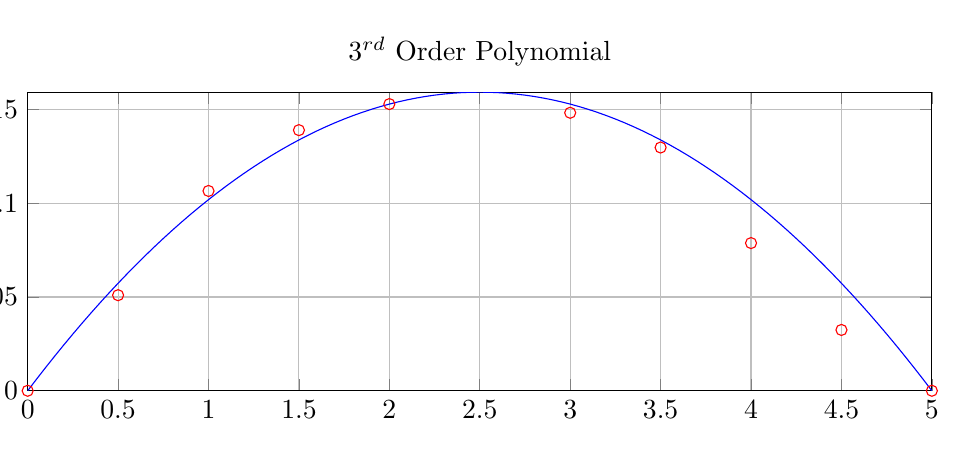
\begin{tikzpicture}[trim axis left, trim axis right]

\begin{axis}[%
width=4.521in,
height=1.493in,
at={(0.758in,2.554in)},
scale only axis,
separate axis lines,
every outer x axis line/.append style={black},
every x tick label/.append style={font=\color{black},/pgf/number format/fixed},
xmin=0,
xmax=5,
xmajorgrids,
every outer y axis line/.append style={black},
every y tick label/.append style={font=\color{black},/pgf/number format/fixed},
ymin=0,
ymax=0.159278747537003,
ylabel={Meter / Second},
ymajorgrids,
axis background/.style={fill=white},
title={$3^{rd}$ Order Polynomial}
]
\addplot [color=blue,solid,forget plot]
  table[row sep=crcr]{%
0	0\\
0.05	0.0063074384024653\\
0.1	0.012487453806901\\
0.15	0.0185400462133071\\
0.2	0.0244652156216836\\
0.25	0.0302629620320305\\
0.3	0.0359332854443478\\
0.35	0.0414761858586355\\
0.4	0.0468916632748935\\
0.45	0.052179717693122\\
0.5	0.0573403491133209\\
0.55	0.0623735575354902\\
0.6	0.0672793429596299\\
0.65	0.0720577053857399\\
0.7	0.0767086448138204\\
0.75	0.0812321612438713\\
0.8	0.0856282546758926\\
0.85	0.0898969251098842\\
0.9	0.0940381725458463\\
0.95	0.0980519969837787\\
1	0.101938398423682\\
1.05	0.105697376865555\\
1.1	0.109328932309399\\
1.15	0.112833064755213\\
1.2	0.116209774202997\\
1.25	0.119459060652752\\
1.3	0.122580924104477\\
1.35	0.125575364558173\\
1.4	0.128442382013839\\
1.45	0.131181976471475\\
1.5	0.133794147931082\\
1.55	0.136278896392659\\
1.6	0.138636221856207\\
1.65	0.140866124321725\\
1.7	0.142968603789213\\
1.75	0.144943660258672\\
1.8	0.146791293730102\\
1.85	0.148511504203501\\
1.9	0.150104291678871\\
1.95	0.151569656156212\\
2	0.152907597635522\\
2.05	0.154118116116804\\
2.1	0.155201211600055\\
2.15	0.156156884085277\\
2.2	0.15698513357247\\
2.25	0.157685960061632\\
2.3	0.158259363552766\\
2.35	0.158705344045869\\
2.4	0.159023901540943\\
2.45	0.159215036037988\\
2.5	0.159278747537003\\
2.55	0.159215036037988\\
2.6	0.159023901540943\\
2.65	0.158705344045869\\
2.7	0.158259363552766\\
2.75	0.157685960061632\\
2.8	0.15698513357247\\
2.85	0.156156884085277\\
2.9	0.155201211600055\\
2.95	0.154118116116804\\
3	0.152907597635522\\
3.05	0.151569656156212\\
3.1	0.150104291678871\\
3.15	0.148511504203501\\
3.2	0.146791293730101\\
3.25	0.144943660258672\\
3.3	0.142968603789213\\
3.35	0.140866124321725\\
3.4	0.138636221856207\\
3.45	0.136278896392659\\
3.5	0.133794147931082\\
3.55	0.131181976471475\\
3.6	0.128442382013839\\
3.65	0.125575364558173\\
3.7	0.122580924104477\\
3.75	0.119459060652752\\
3.8	0.116209774202997\\
3.85	0.112833064755213\\
3.9	0.109328932309399\\
3.95	0.105697376865555\\
4	0.101938398423682\\
4.05	0.0980519969837787\\
4.1	0.0940381725458463\\
4.15	0.0898969251098842\\
4.2	0.0856282546758926\\
4.25	0.0812321612438714\\
4.3	0.0767086448138204\\
4.35	0.07205770538574\\
4.4	0.0672793429596298\\
4.45	0.0623735575354902\\
4.5	0.057340349113321\\
4.55	0.052179717693122\\
4.6	0.0468916632748936\\
4.65	0.0414761858586356\\
4.7	0.0359332854443477\\
4.75	0.0302629620320305\\
4.8	0.0244652156216836\\
4.85	0.0185400462133071\\
4.9	0.012487453806901\\
4.95	0.00630743840246539\\
5	0\\
};
\addplot [color=red,only marks,mark=o,mark options={solid},forget plot]
  table[row sep=crcr]
\noindent\resizebox{0.8\columnwidth}{!}{
% This file was created by matlab2tikz.
%
%The latest updates can be retrieved from
%  http://www.mathworks.com/matlabcentral/fileexchange/22022-matlab2tikz-matlab2tikz
%where you can also make suggestions and rate matlab2tikz.
%
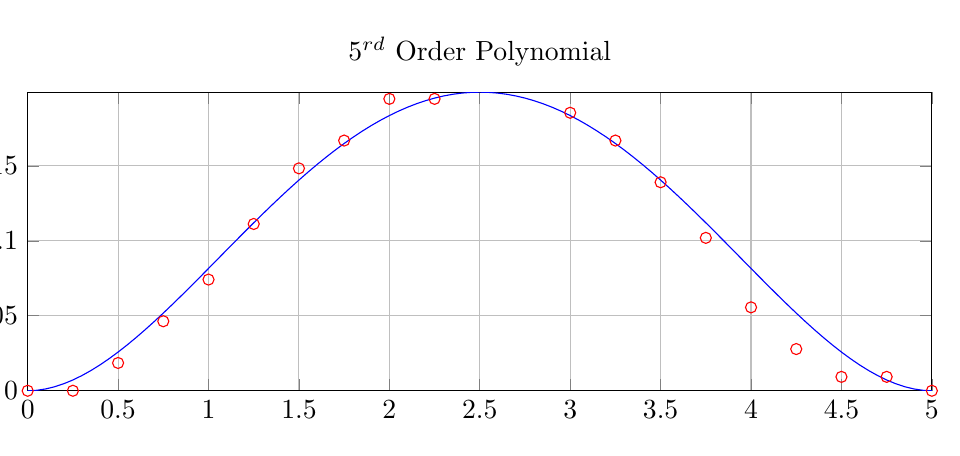
\begin{tikzpicture}[trim axis left, trim axis right]

\begin{axis}[%
width=4.521in,
height=1.493in,
at={(0.758in,2.554in)},
scale only axis,
separate axis lines,
every outer x axis line/.append style={black},
every x tick label/.append style={font=\color{black}},
xmin=0,
xmax=5,
xmajorgrids,
every outer y axis line/.append style={black},
every y tick label/.append style={font=\color{black},/pgf/number format/fixed},
ymin=-4.44089209850063e-16,
ymax=0.199098434421253,
ylabel={Meter / Second},
ymajorgrids,
axis background/.style={fill=white},
title={$5^{rd}$ Order Polynomial}
]
\addplot [color=blue,solid,forget plot]
  table[row sep=crcr]{%
0	0\\
0.05	0.000312218200922032\\
0.1	0.0012237704730763\\
0.15	0.00269757672403618\\
0.2	0.00469732139936325\\
0.25	0.00718745348260724\\
0.3	0.0101331864953061\\
0.35	0.0135004984969858\\
0.4	0.0172561320851608\\
0.45	0.0213675943953335\\
0.5	0.0258031571009944\\
0.55	0.0305318564136224\\
0.6	0.0355234930826846\\
0.65	0.0407486323956359\\
0.7	0.0461786041779199\\
0.75	0.0517855027929679\\
0.8	0.0575421871421998\\
0.85	0.0634222806650233\\
0.9	0.0694001713388346\\
0.95	0.0754510116790177\\
1	0.0815507187389453\\
1.05	0.0876759741099778\\
1.1	0.0938042239214639\\
1.15	0.0999136788407407\\
1.2	0.105983314073133\\
1.25	0.111992869361955\\
1.3	0.117922848988507\\
1.35	0.123754521772079\\
1.4	0.12946992106995\\
1.45	0.135051844777384\\
1.5	0.140483855327636\\
1.55	0.145750279691949\\
1.6	0.150836209379553\\
1.65	0.155727500437667\\
1.7	0.160410773451497\\
1.75	0.16487341354424\\
1.8	0.169103570377077\\
1.85	0.173090158149181\\
1.9	0.17682285559771\\
1.95	0.180292105997814\\
2	0.183489117162627\\
2.05	0.186405861443274\\
2.1	0.189035075728867\\
2.15	0.191370261446507\\
2.2	0.193405684561283\\
2.25	0.19513637557627\\
2.3	0.196558129532535\\
2.35	0.19766750600913\\
2.4	0.198461829123097\\
2.45	0.198939187529466\\
2.5	0.199098434421253\\
2.55	0.198939187529466\\
2.6	0.198461829123097\\
2.65	0.19766750600913\\
2.7	0.196558129532535\\
2.75	0.19513637557627\\
2.8	0.193405684561283\\
2.85	0.191370261446507\\
2.9	0.189035075728867\\
2.95	0.186405861443274\\
3	0.183489117162627\\
3.05	0.180292105997813\\
3.1	0.17682285559771\\
3.15	0.17309015814918\\
3.2	0.169103570377077\\
3.25	0.16487341354424\\
3.3	0.160410773451497\\
3.35	0.155727500437667\\
3.4	0.150836209379553\\
3.45	0.145750279691949\\
3.5	0.140483855327636\\
3.55	0.135051844777384\\
3.6	0.12946992106995\\
3.65	0.123754521772079\\
3.7	0.117922848988507\\
3.75	0.111992869361955\\
3.8	0.105983314073133\\
3.85	0.0999136788407407\\
3.9	0.0938042239214634\\
3.95	0.0876759741099777\\
4	0.081550718738945\\
4.05	0.0754510116790175\\
4.1	0.0694001713388344\\
4.15	0.0634222806650231\\
4.2	0.0575421871421997\\
4.25	0.0517855027929677\\
4.3	0.0461786041779195\\
4.35	0.0407486323956356\\
4.4	0.0355234930826842\\
4.45	0.0305318564136225\\
4.5	0.0258031571009938\\
4.55	0.0213675943953331\\
4.6	0.0172561320851599\\
4.65	0.0135004984969851\\
4.7	0.010133186495306\\
4.75	0.00718745348260663\\
4.8	0.00469732139936285\\
4.85	0.00269757672403648\\
4.9	0.00122377047307598\\
4.95	0.000312218200921865\\
5	-4.44089209850063e-16\\
};
\addplot [color=red,only marks,mark=o,mark options={solid},forget plot]
  table[row sep=crcr]
\noindent\resizebox{0.8\columnwidth}{!}{
% This file was created by matlab2tikz.
%
%The latest updates can be retrieved from
%  http://www.mathworks.com/matlabcentral/fileexchange/22022-matlab2tikz-matlab2tikz
%where you can also make suggestions and rate matlab2tikz.
%
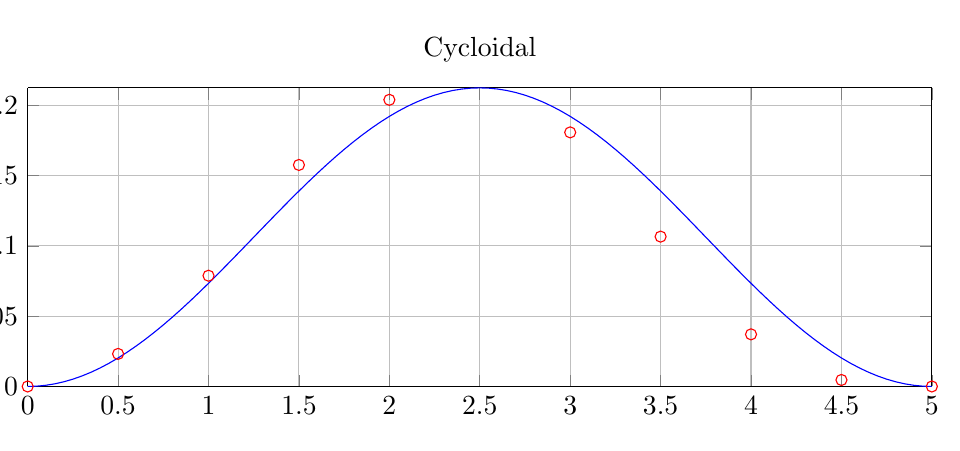
\begin{tikzpicture}[trim axis left, trim axis right]

\begin{axis}[%
width=4.521in,
height=1.493in,
at={(0.758in,2.554in)},
tick label style={/pgf/number format/fixed},
scale only axis,
separate axis lines,
every outer x axis line/.append style={black},
every x tick label/.append style={font=\color{black}},
xmin=0,
xmax=5,
xmajorgrids,
every outer y axis line/.append style={black},
every y tick label/.append style={font=\color{black},/pgf/number format/fixed},
ymin=0,
ymax=0.21237166338267,
ylabel={Meter / Second},
ymajorgrids,
axis background/.style={fill=white},
title={Cycloidal}
]
\addplot [color=blue,solid,forget plot]
  table[row sep=crcr]{%
0	0\\
0.05	0.000209533482996852\\
0.1	0.000837306999056757\\
0.15	0.00188084301291428\\
0.2	0.00333602316466897\\
0.25	0.00519710452307042\\
0.3	0.00745674225024423\\
0.35	0.0101060185884115\\
0.4	0.0131344780542048\\
0.45	0.016530168701684\\
0.5	0.0202796892912071\\
0.55	0.0243682421780003\\
0.6	0.0287796917117015\\
0.65	0.0334966279164008\\
0.7	0.0385004351998614\\
0.75	0.0437713658207576\\
0.8	0.0492886178239878\\
0.85	0.055030417136488\\
0.9	0.0609741034995503\\
0.95	0.0670962198985118\\
1	0.0733726051368746\\
1.05	0.0797784891895106\\
1.1	0.0862885909586342\\
1.15	0.092877218046745\\
1.2	0.0995183681527839\\
1.25	0.106185831691335\\
1.3	0.112853295229886\\
1.35	0.119494445335925\\
1.4	0.126083072424036\\
1.45	0.132593174193159\\
1.5	0.138999058245795\\
1.55	0.145275443484158\\
1.6	0.15139755988312\\
1.65	0.157341246246182\\
1.7	0.163083045558682\\
1.75	0.168600297561912\\
1.8	0.173871228182809\\
1.85	0.178875035466269\\
1.9	0.183591971670968\\
1.95	0.18800342120467\\
2	0.192091974091463\\
2.05	0.195841494680986\\
2.1	0.199237185328465\\
2.15	0.202265644794258\\
2.2	0.204914921132426\\
2.25	0.2071745588596\\
2.3	0.209035640218001\\
2.35	0.210490820369756\\
2.4	0.211534356383613\\
2.45	0.212162129899673\\
2.5	0.21237166338267\\
2.55	0.212162129899673\\
2.6	0.211534356383613\\
2.65	0.210490820369756\\
2.7	0.209035640218001\\
2.75	0.2071745588596\\
2.8	0.204914921132426\\
2.85	0.202265644794258\\
2.9	0.199237185328465\\
2.95	0.195841494680986\\
3	0.192091974091463\\
3.05	0.18800342120467\\
3.1	0.183591971670969\\
3.15	0.178875035466269\\
3.2	0.173871228182809\\
3.25	0.168600297561912\\
3.3	0.163083045558682\\
3.35	0.157341246246182\\
3.4	0.15139755988312\\
3.45	0.145275443484158\\
3.5	0.138999058245795\\
3.55	0.132593174193159\\
3.6	0.126083072424036\\
3.65	0.119494445335925\\
3.7	0.112853295229886\\
3.75	0.106185831691335\\
3.8	0.0995183681527839\\
3.85	0.0928772180467451\\
3.9	0.0862885909586342\\
3.95	0.0797784891895106\\
4	0.0733726051368746\\
4.05	0.0670962198985118\\
4.1	0.0609741034995504\\
4.15	0.055030417136488\\
4.2	0.0492886178239878\\
4.25	0.0437713658207576\\
4.3	0.0385004351998614\\
4.35	0.0334966279164009\\
4.4	0.0287796917117015\\
4.45	0.0243682421780003\\
4.5	0.0202796892912071\\
4.55	0.016530168701684\\
4.6	0.0131344780542048\\
4.65	0.0101060185884115\\
4.7	0.00745674225024422\\
4.75	0.00519710452307042\\
4.8	0.00333602316466898\\
4.85	0.0018808430129143\\
4.9	0.000837306999056757\\
4.95	0.000209533482996852\\
5	0\\
};
\addplot [color=red,only marks,mark=o,mark options={solid},forget plot]
  table[row sep=crcr]
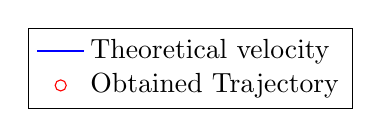
\begin{tikzpicture}
    \begin{customlegend}[legend entries={Theoretical velocity,Obtained Trajectory},legend cell align=left]
    \addlegendimage{blue,fill=blue,sharp plot}
    \addlegendimage{red,mark=o,only marks}
    \end{customlegend}
\end{tikzpicture}
\caption{Speed measured on different interpolators}
\label{fig:vel}
\end{figure}

The interpolators used, as mentioned before, are the $3^{rd}$ and $5^{th}$ order polynomial, as well as the cycloidal interpolator.
The objective of this stage of testing was to study their influence on the trajectory of the robot, and try to verify if the use of interpolators would produce better results than a simple control with no interpolators whatsoever.

This results can be appreciated on figure \ref{fig:vel} (Velocity curves) and \ref{fig:trayint} (Obtained trajectories), where it can be seen that the use of interpolators creates better trajectories, much closer to the desired theoretical results, in both the magnitude of the wheels' speed, but also the obtained final trajectories.

\begin{figure}[h]
\centering
\noindent\resizebox{0.8\columnwidth}{!}{
% This file was created by matlab2tikz.
%
%The latest updates can be retrieved from
%  http://www.mathworks.com/matlabcentral/fileexchange/22022-matlab2tikz-matlab2tikz
%where you can also make suggestions and rate matlab2tikz.
%
\definecolor{mycolor1}{rgb}{1.00000,0.00000,1.00000}%
%
\begin{tikzpicture}[trim axis left, trim axis right]

\begin{axis}[%
width=4.521in,
height=4.521in,
at={(0.758in,0.481in)},
scale only axis,
separate axis lines,
every outer x axis line/.append style={black},
every x tick label/.append style={font=\color{black},/pgf/number format/fixed},
xmin=-0.2,
xmax=0.2,
xlabel={Meters},
xmajorgrids,
every outer y axis line/.append style={black},
every y tick label/.append style={font=\color{black},/pgf/number format/fixed},
ymin=-0.2,
ymax=0.2,
ylabel={Meters},
ymajorgrids,
axis background/.style={fill=white},
]
\addplot [color=black,only marks,mark=x,mark options={solid},forget plot]
  table[row sep=crcr]{%
0.15	0\\
0.149988156630572	0.00188490598250289\\
0.149893420896088	0.00565352740049018\\
0.149573835039092	0.0112990208291899\\
0.148817205197172	0.0187999850346456\\
0.147343087609303	0.0281071971878587\\
0.144807245824991	0.0391262259434845\\
0.140810078648081	0.0516964384761775\\
0.134910787734956	0.0655673649976399\\
0.126649188825302	0.0803740192468495\\
0.115576986416368	0.0956135984623034\\
0.101299921218154	0.110626967603726\\
0.0835313424732281	0.124589384879372\\
0.0621563371489925	0.136515895602749\\
0.0373034830747281	0.145287474169295\\
0.00941857792939688	0.149704009264241\\
-0.0206685436026958	0.148569213854498\\
-0.0516964384761777	0.140810078648081\\
-0.0819591520101405	0.125629206006321\\
-0.109345294113212	0.102682065889303\\
-0.13144600200658	0.0722630511152572\\
-0.145744759937201	0.0354748495535586\\
-0.149893420896088	-0.00565352740049031\\
-0.142064745749212	-0.0481415414710815\\
-0.121352549156242	-0.0881677878438711\\
-0.088167787843871	-0.121352549156242\\
-0.0445562372365553	-0.143229681711997\\
0.00565352740049011	-0.149893420896089\\
0.0569668643282701	-0.138761581025169\\
0.102682065889303	-0.109345294113212\\
0.135724057869903	-0.0638668937347611\\
0.149810543490903	-0.00753664772696559\\
0.140810078648081	0.0516964384761774\\
0.108046353733186	0.104047995871921\\
0.0552186829027014	0.139466472883237\\
-0.00941857792939727	0.14970400926424\\
-0.073909101232244	0.130527563200428\\
-0.124589384879372	0.0835313424732277\\
-0.149041696578001	0.0169284577310217\\
-0.139466472883238	-0.0552186829027022\\
-0.0956135984623034	-0.115576986416369\\
-0.0262534588462913	-0.147684650179381\\
0.0516964384761776	-0.140810078648081\\
0.116769345235053	-0.0941537041936051\\
0.148817205197171	-0.0187999850346456\\
0.135724057869902	0.0638668937347609\\
0.0787761944941938	0.127649172269204\\
-0.0056535274004908	0.149893420896088\\
-0.0896857474586284	0.120235047730631\\
-0.142658477444273	0.0463525491562415\\
-0.142658477444273	-0.0463525491562427\\
-0.0866359055133401	-0.122450887607578\\
0.00565352740049033	-0.149893420896089\\
0.0970583942354168	-0.114366376651717\\
0.147343087609303	-0.0281071971878588\\
0.131446002006579	0.0722630511152571\\
0.0534617818069872	0.140149341368492\\
-0.0516964384761779	0.140810078648081\\
-0.132343683965243	0.0706055898247994\\
-0.145287474169295	-0.0373034830747287\\
-0.0803740192468491	-0.126649188825303\\
0.0299564970771614	-0.146978257857637\\
0.124589384879372	-0.0835313424732282\\
0.146978257857637	0.0299564970771611\\
0.0803740192468494	0.126649188825302\\
-0.0373034830747284	0.145287474169294\\
-0.132343683965243	0.0706055898247994\\
-0.140810078648081	-0.051696438476178\\
-0.0534617818069871	-0.140149341368492\\
0.0722630511152578	-0.131446002006579\\
0.147343087609303	-0.0281071971878582\\
0.114366376651717	0.097058394235417\\
-0.00565352740049099	0.149893420896088\\
-0.122450887607578	0.0866359055133389\\
-0.142658477444273	-0.0463525491562435\\
-0.046352549156241	-0.142658477444274\\
0.0896857474586288	-0.120235047730632\\
0.149893420896089	0.00565352740048995\\
0.0787761944941954	0.127649172269204\\
-0.0638668937347598	0.135724057869903\\
-0.14881720519717	0.0187999850346452\\
-0.094153704193603	-0.116769345235054\\
0.0516964384761797	-0.140810078648081\\
0.147684650179382	-0.0262534588462905\\
0.0956135984623045	0.115576986416369\\
-0.0552186829027007	0.139466472883238\\
-0.149041696578	0.0169284577310227\\
-0.0835313424732279	-0.124589384879372\\
0.073909101232244	-0.130527563200429\\
0.149704009264241	0.00941857792939722\\
0.0552186829027014	0.139466472883238\\
-0.104047995871921	0.108046353733185\\
-0.140810078648081	-0.0516964384761783\\
-0.00753664772696475	-0.149810543490903\\
0.135724057869904	-0.0638668937347612\\
0.109345294113213	0.102682065889303\\
-0.0569668643282691	0.138761581025169\\
-0.149893420896088	-0.00565352740048949\\
-0.0445562372365543	-0.143229681711996\\
0.121352549156243	-0.0881677878438699\\
0.121352549156242	0.0881677878438721\\
-0.0481415414710817	0.142064745749211\\
-0.149893420896087	-0.0056535274004917\\
-0.0354748495535555	-0.145744759937201\\
0.131446002006582	-0.0722630511152551\\
0.102682065889303	0.109345294113213\\
-0.0819591520101412	0.125629206006321\\
-0.140810078648079	-0.0516964384761789\\
0.0206685436026983	-0.148569213854498\\
0.149704009264242	-0.0094185779293956\\
0.0373034830747268	0.145287474169294\\
-0.136515895602749	0.0621563371489893\\
-0.0835313424732242	-0.124589384879374\\
0.11062696760373	-0.101299921218152\\
0.115576986416367	0.0956135984623052\\
-0.0803740192468511	0.1266491888253\\
-0.134910787734953	-0.0655673649976432\\
0.0516964384761814	-0.140810078648081\\
0.144807245824992	0.0391262259434859\\
-0.0281071971878591	0.147343087609303\\
-0.14881720519717	-0.0187999850346471\\
0.0112990208291931	-0.149573835039091\\
0.14989342089609	0.00565352740049296\\
-0.00188490598250418	0.149988156630573\\
-0.149999999999999	-1.73038666728687e-15\\
3.03704771181041e-15	-0.149999999999999\\
0.149988156630574	0.00188490598250505\\
-0.00565352740049035	0.149893420896089\\
-0.149573835039092	-0.0112990208291901\\
0.0187999850346467	-0.148817205197171\\
0.147343087609303	0.0281071971878603\\
-0.039126225943486	0.144807245824991\\
-0.14081007864808	-0.0516964384761785\\
0.0655673649976414	-0.134910787734955\\
0.126649188825302	0.0803740192468508\\
-0.0956135984623044	0.115576986416369\\
-0.101299921218153	-0.110626967603726\\
0.124589384879372	-0.0835313424732283\\
0.0621563371489934	0.136515895602749\\
-0.145287474169293	0.0373034830747274\\
-0.00941857792939545	-0.149704009264241\\
0.148569213854498	0.0206685436026961\\
-0.0516964384761773	0.140810078648081\\
-0.125629206006323	-0.0819591520101398\\
0.10934529411321	-0.102682065889306\\
0.0722630511152583	0.131446002006577\\
-0.145744759937201	0.0354748495535577\\
0.00565352740049201	-0.149893420896088\\
0.142064745749214	0.0481415414710815\\
-0.0881677878438688	0.121352549156243\\
-0.0881677878438684	-0.121352549156241\\
0.143229681711998	-0.0445562372365517\\
-0.00565352740048871	0.149893420896092\\
-0.138761581025168	-0.0569668643282661\\
0.102682065889304	-0.109345294113208\\
0.0638668937347602	0.135724057869906\\
-0.149810543490901	0.00753664772696471\\
0.0516964384761806	-0.14081007864808\\
0.108046353733187	0.104047995871922\\
-0.139466472883236	0.0552186829027004\\
0.00941857792940338	-0.149704009264239\\
0.130527563200433	0.0739091012322472\\
-0.124589384879368	0.0835313424732301\\
-0.0169284577310168	-0.149041696577999\\
0.13946647288324	0.0552186829027067\\
-0.115576986416366	0.0956135984623084\\
-0.0262534588462909	-0.147684650179377\\
0.140810078648084	0.0516964384761801\\
-0.116769345235051	0.094153704193609\\
-0.0187999850346417	-0.148817205197167\\
0.135724057869908	0.0638668937347643\\
-0.127649172269198	0.0787761944942008\\
0.00565352740049338	-0.149893420896083\\
0.120235047730635	0.0896857474586326\\
-0.142658477444269	0.0463525491562439\\
0.046352549156247	-0.142658477444271\\
0.0866359055133447	0.12245088760758\\
-0.149893420896083	-0.00565352740048905\\
0.0970583942354238	-0.114366376651712\\
0.0281071971878644	0.147343087609308\\
-0.131446002006574	-0.0722630511152526\\
0.140149341368498	-0.0534617818069824\\
-0.0516964384761736	0.140810078648085\\
-0.0706055898247896	-0.13234368396524\\
0.145287474169302	0.0373034830747345\\
-0.126649188825295	0.0803740192468521\\
0.0299564970771723	-0.146978257857632\\
0.0835313424732316	0.124589384879379\\
-0.146978257857631	-0.0299564970771581\\
0.126649188825309	-0.0803740192468432\\
-0.0373034830747246	0.145287474169299\\
-0.0706055898247903	-0.13234368396524\\
0.140810078648084	0.0516964384761884\\
-0.140149341368489	0.0534617818069906\\
0.072263051115265	-0.131446002006571\\
0.028107197187858	0.14734308760931\\
-0.114366376651708	-0.0970583942354154\\
0.149893420896095	0.00565352740049944\\
-0.122450887607573	0.0866359055133425\\
0.0463525491562525	-0.142658477444266\\
0.0463525491562426	0.14265847744428\\
-0.12023504773062	-0.089685747458629\\
0.149893420896094	0.00565352740050773\\
-0.127649172269206	0.0787761944941853\\
0.0638668937347745	-0.135724057869898\\
0.0187999850346437	0.148817205197174\\
-0.0941537041935954	-0.116769345235056\\
0.140810078648084	0.051696438476184\\
-0.147684650179377	0.0262534588462862\\
0.115576986416378	-0.095613598462296\\
-0.0552186829027063	0.139466472883235\\
-0.0169284577310029	-0.149041696578001\\
0.0835313424732175	0.124589384879383\\
-0.130527563200422	-0.0739091012322511\\
0.149704009264241	0.00941857792940888\\
-0.13946647288324	0.055218682902697\\
0.104047995871927	-0.108046353733178\\
-0.0516964384761844	0.140810078648081\\
-0.0075366477269541	-0.1498105434909\\
0.0638668937347504	0.135724057869911\\
-0.109345294113199	-0.102682065889312\\
0.138761581025162	0.056966864328292\\
-0.149893420896089	-0.00565352740049735\\
0.143229681711999	-0.0445562372365381\\
-0.121352549156249	0.088167787843869\\
0.0881677878438779	-0.12135254915623\\
-0.0481415414710927	0.142064745749214\\
0.00565352740050146	-0.149893420896081\\
0.035474849553543	0.145744759937211\\
-0.072263051115242	-0.131446002006582\\
0.102682065889285	0.109345294113234\\
-0.125629206006317	-0.0819591520101449\\
0.140810078648072	0.0516964384761992\\
-0.148569213854501	-0.0206685436026993\\
0.149704009264237	-0.00941857792937601\\
-0.145287474169302	0.0373034830747243\\
0.136515895602751	-0.0621563371489705\\
-0.124589384879386	0.0835313424732224\\
0.110626967603736	-0.101299921218129\\
-0.0956135984623275	0.115576986416361\\
0.0803740192468572	-0.126649188825287\\
-0.0655673649976621	0.134910787734954\\
0.0516964384761838	-0.14081007864807\\
-0.0391262259435065	0.144807245824993\\
0.0281071971878661	-0.147343087609295\\
-0.0187999850346704	0.148817205197175\\
0.0112990208292018	-0.149573835039085\\
-0.00565352740052136	0.149893420896093\\
0.00188490598252291	-0.149988156630566\\
-2.42540362793697e-14	0.150000000000006\\
1.48335467710866e-14	-0.149999999999994\\
-0.00188490598252386	0.149988156630578\\
0.00565352740050375	-0.149893420896082\\
-0.0112990208292113	0.149573835039097\\
0.0187999850346615	-0.148817205197163\\
-0.0281071971878841	0.147343087609305\\
0.0391262259435061	-0.144807245824979\\
-0.0516964384762096	0.140810078648077\\
0.0655673649976531	-0.134910787734941\\
-0.0803740192468747	0.126649188825296\\
0.0956135984623113	-0.115576986416351\\
-0.110626967603747	0.101299921218144\\
0.124589384879376	-0.0835313424732065\\
-0.136515895602766	0.0621563371489771\\
0.145287474169294	-0.0373034830746995\\
-0.14970400926425	0.00941857792937329\\
0.148569213854486	0.0206685436027332\\
-0.14081007864808	-0.0516964384761927\\
0.125629206006301	0.0819591520101692\\
-0.102682065889294	-0.109345294113218\\
0.0722630511152301	0.131446002006599\\
-0.0354748495535439	-0.145744759937198\\
-0.00565352740052268	0.149893420896097\\
0.0481415414710999	-0.142064745749194\\
-0.0881677878439041	0.121352549156233\\
0.121352549156256	-0.0881677878438332\\
-0.143229681712009	0.0445562372365402\\
0.149893420896083	0.00565352740052881\\
-0.138761581025164	-0.0569668643282812\\
0.10934529411319	0.102682065889334\\
-0.0638668937347422	-0.135724057869902\\
0.00753664772693312	0.149810543490917\\
0.0516964384762014	-0.140810078648059\\
-0.10404799587195	0.108046353733175\\
0.139466472883248	-0.0552186829026539\\
-0.149704009264241	-0.00941857792941241\\
0.130527563200412	0.0739091012322848\\
-0.0835313424732071	-0.124589384879372\\
0.0169284577309767	0.149041696578026\\
0.0552186829027271	-0.139466472883204\\
-0.115576986416389	0.0956135984623038\\
0.147684650179386	-0.0262534588462351\\
-0.140810078648072	-0.0516964384761722\\
0.0941537041935801	0.116769345235107\\
-0.0187999850346226	-0.148817205197139\\
-0.0638668937348008	0.135724057869926\\
0.127649172269209	-0.0787761944941312\\
-0.149893420896102	-0.00565352740050008\\
0.120235047730592	0.0896857474586896\\
-0.0463525491562308	-0.142658477444247\\
-0.046352549156297	0.142658477444299\\
0.122450887607568	-0.0866359055132815\\
-0.149893420896116	-0.00565352740049251\\
0.114366376651669	0.0970583942354673\\
-0.0281071971878484	-0.147343087609287\\
-0.0722630511153112	0.131446002006586\\
0.14014934136849	-0.0534617818069212\\
-0.140810078648083	-0.0516964384761913\\
0.0706055898247541	0.132343683965279\\
0.0373034830747524	-0.145287474169267\\
-0.126649188825327	0.080374019246842\\
0.146978257857625	0.0299564970772203\\
-0.0835313424732064	-0.124589384879364\\
-0.0299564970772103	0.146978257857659\\
0.12664918882531	-0.0803740192467879\\
-0.1452874741693	-0.0373034830747493\\
0.0706055898247426	0.132343683965288\\
0.0516964384761908	-0.140810078648041\\
-0.140149341368532	0.0534617818069754\\
0.131446002006535	0.0722630511153096\\
-0.0281071971878447	-0.147343087609293\\
-0.097058394235466	0.114366376651711\\
0.14989342089607	0.00565352740055342\\
-0.086635905513324	-0.122450887607579\\
-0.0463525491563121	0.142658477444285\\
0.142658477444265	-0.0463525491561682\\
-0.120235047730627	-0.0896857474586274\\
-0.00565352740055675	0.149893420896123\\
0.127649172269196	-0.0787761944941257\\
-0.135724057869915	-0.0638668937347678\\
0.0187999850345779	0.148817205197206\\
0.11676934523506	-0.0941537041935414\\
-0.140810078648087	-0.0516964384761896\\
0.0262534588462159	0.147684650179427\\
0.115576986416378	-0.0956135984622263\\
-0.13946647288324	-0.0552186829027014\\
0.0169284577309549	0.149041696578051\\
0.12458938487937	-0.0835313424731481\\
-0.130527563200434	-0.0739091012322424\\
-0.00941857792946596	0.149704009264277\\
0.139466472883236	-0.0552186829026171\\
-0.108046353733173	-0.104047995871914\\
-0.0516964384762546	0.140810078648108\\
0.149810543490881	-0.00753664772686331\\
-0.0638668937347412	-0.13572405786987\\
-0.102682065889367	0.109345294113231\\
0.138761581025121	0.0569668643283631\\
0.00565352740051135	-0.14989342089604\\
-0.143229681712035	0.0445562372365581\\
0.0881677878438053	0.121352549156326\\
0.0881677878438876	-0.121352549156158\\
-0.142064745749224	-0.0481415414710881\\
-0.00565352740058054	0.149893420896136\\
0.145744759937175	-0.035474849553459\\
-0.0722630511152485	-0.131446002006559\\
-0.109345294113279	0.102682065889312\\
0.125629206006261	0.0819591520102323\\
0.0516964384761913	-0.140810078648014\\
-0.148569213854529	-0.020668543602703\\
0.00941857792930408	0.149704009264291\\
0.14528747416928	-0.0373034830746216\\
-0.0621563371489661	-0.13651589560273\\
-0.124589384879427	0.0835313424732247\\
0.101299921218088	0.11062696760381\\
0.0956135984623173	-0.115576986416287\\
-0.126649188825302	-0.080374019246852\\
-0.0655673649977162	0.134910787734975\\
0.140810078648038	0.0516964384762788\\
0.0391262259435174	-0.144807245824929\\
-0.147343087609322	-0.028107197187879\\
-0.0187999850347427	0.148817205197208\\
0.149573835039049	0.011299020829293\\
0.00565352740051386	-0.149893420896044\\
-0.149988156630604	-0.00188490598251733\\
-9.32431215572294e-14	0.150000000000046\\
0.149999999999964	1.03262695349122e-13\\
0.00188490598253011	-0.149988156630532\\
-0.149893420896121	-0.00565352740051196\\
-0.0112990208292943	0.149573835039135\\
0.148817205197128	0.0187999850347634\\
0.0281071971878853	-0.147343087609236\\
-0.144807245825012	-0.0391262259434929\\
-0.0516964384762703	0.14081007864811\\
0.134910787734895	0.0655673649977489\\
0.0803740192468672	-0.126649188825215\\
-0.115576986416365	-0.0956135984623043\\
-0.110626967603808	0.101299921218155\\
0.0835313424731344	0.124589384879469\\
0.136515895602748	-0.0621563371488699\\
-0.0373034830746928	-0.145287474169249\\
-0.149704009264277	0.00941857792939041\\
-0.020668543602791	0.148569213854546\\
0.14081007864803	0.0516964384762994\\
0.0819591520101658	-0.125629206006225\\
-0.102682065889286	-0.109345294113203\\
-0.131446002006646	0.072263051115253\\
0.0354748495534543	0.145744759937283\\
0.149893420896057	0.00565352740063164\\
0.0481415414711196	-0.142064745749118\\
-0.12135254915623	-0.0881677878438602\\
-0.12135254915631	0.0881677878438817\\
0.0445562372364608	0.143229681712087\\
0.149893420896057	0.00565352740062897\\
0.056966864328311	-0.138761581025076\\
-0.109345294113189	-0.102682065889292\\
-0.13572405786997	0.0638668937347575\\
0.00753664772686099	0.149810543490961\\
0.140810078648014	0.0516964384762876\\
0.104047995871918	-0.108046353733091\\
-0.0552186829026892	-0.139466472883219\\
-0.14970400926428	-0.00941857792941525\\
-0.0739091012323347	0.130527563200439\\
0.0835313424731397	0.124589384879447\\
0.149041696577986	-0.0169284577309134\\
0.0552186829027423	-0.139466472883172\\
-0.0956135984622738	-0.115576986416372\\
-0.147684650179426	0.0262534588462605\\
-0.0516964384762716	0.140810078648091\\
0.0941537041935206	0.116769345235121\\
0.148817205197144	-0.018799985034555\\
0.0638668937347937	-0.135724057869856\\
-0.0787761944941652	-0.12764917226922\\
-0.149893420896112	-0.00565352740053658\\
-0.0896857474587124	0.120235047730614\\
0.0463525491561492	0.142658477444307\\
0.142658477444212	0.0463525491563073\\
0.122450887607562	-0.0866359055132819\\
0.00565352740050093	-0.149893420896079\\
-0.114366376651724	-0.0970583942354481\\
-0.14734308760935	0.0281071971878168\\
-0.0722630511153403	0.131446002006564\\
0.0534617818069006	0.140149341368534\\
0.140810078648029	0.0516964384762552\\
0.132343683965241	-0.0706055898247257\\
0.0373034830747609	-0.145287474169265\\
-0.0803740192468238	-0.126649188825316\\
-0.146978257857644	-0.0299564970771976\\
-0.12458938487942	0.0835313424731999\\
-0.0299564970772383	0.146978257857652\\
0.0803740192467801	0.12664918882536\\
0.145287474169259	0.0373034830748099\\
0.132343683965253	-0.0706055898247238\\
0.0516964384762102	-0.140810078648031\\
-0.0534617818069553	-0.14014934136847\\
-0.131446002006567	-0.0722630511152577\\
-0.147343087609327	0.0281071971878524\\
-0.0970583942354647	0.114366376651725\\
-0.00565352740054735	0.14989342089612\\
0.0866359055132911	0.122450887607637\\
0.142658477444255	0.0463525491563241\\
0.142658477444287	-0.0463525491561601\\
0.0896857474586673	-0.120235047730568\\
0.00565352740054184	-0.14989342089606\\
-0.0787761944941497	-0.127649172269202\\
-0.135724057869876	-0.0638668937347751\\
-0.148817205197171	0.0187999850346274\\
-0.116769345235083	0.0941537041935998\\
-0.0516964384762224	0.140810078648097\\
0.0262534588462443	0.147684650179422\\
0.0956135984622684	0.115576986416436\\
0.139466472883219	0.0552186829027804\\
0.149041696577998	-0.0169284577309415\\
0.124589384879384	-0.0835313424731531\\
0.0739091012322707	-0.13052756320037\\
0.00941857792942824	-0.149704009264196\\
-0.0552186829026725	-0.139466472883207\\
-0.108046353733166	-0.104047995871903\\
-0.140810078648079	-0.051696438476171\\
-0.149810543490918	0.00753664772696952\\
-0.135724057869935	0.0638668937347691\\
-0.102682065889352	0.109345294113232\\
-0.0569668643283264	0.138761581025201\\
-0.00565352740054888	0.149893420896133\\
0.0445562372364982	0.143229681712054\\
0.0881677878438216	0.121352549156315\\
0.121352549156202	0.0881677878439527\\
0.142064745749182	0.0481415414711687\\
0.149893420896073	0.00565352740057983\\
0.145744759937194	-0.0354748495534699\\
0.131446002006579	-0.0722630511151709\\
0.109345294113217	-0.102682065889221\\
0.0819591520101512	-0.125629206006246\\
0.0516964384761912	-0.140810078648011\\
0.0206685436027105	-0.148569213854433\\
-0.00941857792938201	-0.149704009264182\\
-0.0373034830747147	-0.145287474169244\\
-0.0621563371489812	-0.136515895602705\\
-0.0835313424732197	-0.124589384879333\\
-0.10129992121815	-0.110626967603692\\
-0.115576986416368	-0.0956135984622727\\
-0.126649188825304	-0.0803740192468207\\
-0.134910787734961	-0.0655673649976129\\
-0.14081007864809	-0.0516964384761523\\
-0.144807245825003	-0.03912622594346\\
-0.147343087609318	-0.0281071971878347\\
-0.148817205197189	-0.0187999850346221\\
-0.149573835039111	-0.0112990208291664\\
-0.149893420896107	-0.00565352740046662\\
-0.149988156630592	-0.00188490598247941\\
-0.15000000000002	2.35332586751014e-14\\
-0.15000000000002	2.35699980790758e-14\\
};
\addplot [color=blue,solid,forget plot]
  table[row sep=crcr]{%
-0.15	0\\
-0.15	0\\
-0.140855037033719	0.0486764532340187\\
-0.0952966889970419	0.116353114824504\\
0.0219523249226854	0.15456623817601\\
0.13209975994468	0.0770101842940635\\
0.122209277639044	-0.0671557689329328\\
0.00312956229544044	-0.127291331666595\\
-0.0954500488630746	-0.0917604247549201\\
-0.137852405244662	-0.0417352788077643\\
-0.150099569417224	-0.00811957152294495\\
};
\addplot [color=red,solid,forget plot]
  table[row sep=crcr]{%
-0.15	0\\
-0.15	0\\
-0.14825187926356	0.0219179509839571\\
-0.123089470188904	0.0848692003712424\\
-0.00877033433949519	0.151436134865835\\
0.13909907637152	0.0675153808573533\\
0.106339370024418	-0.109043251294718\\
-0.0329073932902801	-0.150714150512363\\
-0.117438464379485	-0.102000169755891\\
-0.135789562514726	-0.0739479842982829\\
-0.139492932837836	-0.0654571239930683\\
};
\addplot [color=green,solid,forget plot]
  table[row sep=crcr]{%
-0.15	0\\
-0.15	0\\
-0.150501341652883	0.00808853590427871\\
-0.140872534241904	0.0854646606570109\\
-0.0506987558346754	0.176945372480734\\
0.114503075593127	0.125123491864887\\
0.111856733282016	-0.0462784337701122\\
-0.0324288128588738	-0.103775691112415\\
-0.120155742221754	-0.0511316188331386\\
-0.142391594965844	-0.00953126432502029\\
-0.145081200019578	0.0017312229288515\\
};
\addplot [color=mycolor1,only marks,mark=x,mark options={solid},forget plot]
  table[row sep=crcr]{%
-0.121239602002359	0.00920097104914458\\
-0.11846251995298	0.0273921581538884\\
-0.109246081852831	0.0533759549023928\\
-0.0883443340391121	0.0835402753474245\\
-0.0511957777552311	0.110284592314497\\
0.00241476733279171	0.121564254041499\\
0.0635609920758673	0.103651817390093\\
0.111279599181233	0.0489954055805428\\
0.11728125695835	-0.0320750016088409\\
0.063177001101318	-0.1038863104253\\
-0.0343979052076327	-0.116621109063773\\
-0.113137549457316	-0.0445375556663269\\
-0.0996828619501075	0.0696205860028018\\
0.0120547936493123	0.120989176838303\\
0.114817001372414	0.040009438358776\\
0.0777859051559371	-0.0934507994669349\\
-0.0680005820920238	-0.100794939342626\\
-0.112636163402002	0.0457907595046784\\
0.03061114937015	0.11767181691542\\
0.119197904526079	-0.0239908007062992\\
-0.0263533637934241	-0.118697932495512\\
-0.115640120616211	0.0375640980965333\\
0.0567323967639393	0.107541313546733\\
0.0903986171787213	-0.0813129077952124\\
-0.105792341801277	-0.0599306213728808\\
-0.0141726163101856	0.120759413334373\\
0.11390046204512	-0.042548604064599\\
-0.0958140931646393	-0.0748555843806963\\
-0.0045441446108065	0.121503290950055\\
0.0957405577041534	-0.0749496135576121\\
-0.120573443085162	-0.015676217162537\\
0.0805178870194798	0.0911074576083429\\
-0.00993327068171414	-0.121181801833037\\
-0.0566267910030636	0.107596958612375\\
0.10063546774555	-0.0682363656239987\\
-0.119599917607606	0.0218988280552056\\
0.120075440332072	0.0191203449497333\\
-0.110962801337172	-0.0497087083049343\\
0.0997511637510137	0.0695226890464989\\
-0.091374502071684	-0.0802147077105535\\
0.0884263069250788	0.0834535032549832\\
-0.0916707049938819	-0.0798760340018356\\
0.100262955435949	0.0687825466901793\\
-0.111507783938494	-0.0484738391615914\\
0.120345290764734	0.0173409905336853\\
-0.119174294173179	0.0241078113951136\\
0.0990957639665662	-0.0704537332284125\\
-0.0538210185203537	0.109027505370752\\
-0.0135157961985927	-0.120834689617907\\
0.0835069109899683	0.0883758721532706\\
-0.121070856272456	-0.0112047634241907\\
0.092611289030898	-0.0787835522553609\\
0.000853940232771515	0.121585236554512\\
-0.099302837238471	-0.07016156696032\\
0.111544359122714	-0.0483896157232177\\
-0.00745129763429652	0.121359701406615\\
-0.109153206366779	-0.0535656279883751\\
0.0851079989735856	-0.0868350590064282\\
0.0637643892888676	0.103526815949084\\
-0.112715529174458	0.0455950484686614\\
-0.0350578836224432	-0.116424412207462\\
0.11697575716423	-0.0331718434488152\\
0.0400787980236017	0.114792808620231\\
-0.108335910911611	0.0551999037036231\\
-0.0766724651386115	-0.0943664773715016\\
0.068820400603655	-0.100236976324559\\
0.118129426252537	0.0287947497850586\\
0.0240628100276592	0.119183388672711\\
-0.0919476307804544	0.0795570999710205\\
-0.117257000779312	-0.0321635621500182\\
-0.0471060497226529	-0.112092457558324\\
0.0508707412412579	-0.110434897779202\\
0.112670712028276	-0.0457056846899714\\
0.116419115803089	0.0350754677454878\\
0.0760651399509389	0.0948566995324094\\
0.0180949790317856	0.120234232628553\\
-0.0360939647772631	0.116107384212183\\
-0.0761152737378984	0.0948164757082993\\
-0.100686970501729	0.0681603472197851\\
-0.113291584452784	0.0441442618481202\\
-0.118556961944525	0.0269804695367269\\
-0.120191541196429	0.0183764084294194\\
-0.120122717768398	0.0188210424225541\\
-0.118250144445315	0.0282949165151601\\
-0.112455475477608	0.0462327264720873\\
-0.0988878310933417	0.0707452883490656\\
-0.0729158910196207	0.097298364830826\\
-0.0313392478531121	0.117480000450881\\
0.0238557596475012	0.119225004481352\\
0.0812104533755917	0.0904906692674365\\
0.118393887370004	0.0276872966422594\\
0.109181507692781	-0.0535079184781926\\
0.0421440591029608	-0.114050766083634\\
-0.0564642140639775	-0.107682363885991\\
-0.119726836683964	-0.0211939505422909\\
-0.0835536177555886	0.0883317152663227\\
0.0366897319849818	0.115920500899573\\
0.12064894057851	0.015084167170279\\
0.0560979455585366	-0.107873627296245\\
-0.0882180556677102	-0.0836736136195067\\
-0.0997879018254549	0.0694699475400053\\
0.0561712512242997	0.107835474208789\\
0.110618573911215	-0.0504700908240404\\
-0.0530622294395111	-0.109398806066823\\
-0.103598980906189	0.0636470746942607\\
0.0807172238866326	0.0909309008531915\\
0.0680538561574522	-0.100758977883058\\
-0.117264284655335	-0.0321369959114162\\
0.0163406838243827	0.120485190019725\\
0.0994615383063509	-0.0699364093993395\\
-0.111791382235772	-0.0478161669287002\\
0.0271684550311572	0.118514024542067\\
0.0726290078423904	-0.0975126975412316\\
-0.120384269132321	0.0170682953869041\\
0.102155453179695	0.0659390805788869\\
-0.0427549737893844	-0.113823157477759\\
-0.024539648699773	0.119086122632444\\
0.0773970829139804	-0.0937730799235269\\
-0.108419160199601	0.0550362122929157\\
0.120491351595235	-0.0162951880225789\\
-0.120637514755399	-0.0151752757990936\\
0.11583149773458	0.0369697591891239\\
-0.11116831108687	-0.0492473915251413\\
0.109518741483568	0.0528142426414806\\
-0.111708159913699	-0.0480102694288757\\
0.116623706428475	0.0343890979937332\\
-0.12107592088241	-0.0111499033365414\\
0.119649223986655	-0.0216278099059721\\
-0.10519888551016	0.0609663304567207\\
0.0709840548354076	-0.0987165787548453\\
-0.0152208268712483	0.120631776043019\\
-0.052681872090867	-0.109582477225783\\
0.108223132380061	0.0554206872908086\\
-0.11775231615098	0.0303000165514383\\
0.0602100385155647	-0.105633565801273\\
0.0426690034337165	0.113855413169121\\
-0.117505993726586	-0.0312416452874241\\
0.0874370299140009	-0.0844894357997248\\
0.0360851963544572	0.11611010966319\\
-0.121097580259563	-0.0109121499813952\\
0.0479427719144753	-0.111737145046284\\
0.0971605280267218	0.0730994579699899\\
-0.0879775725637091	0.0839264302096486\\
-0.075850040273784	-0.0950287869669137\\
0.0959665255007574	-0.0746600625853621\\
0.0805797915581681	0.0910527108568433\\
-0.0790071273320943	0.0924206296920117\\
-0.107135875851928	-0.0574943742237276\\
0.0243957384793097	-0.119115687069281\\
0.119951733328934	-0.0198816657582286\\
0.0692814266416064	0.0999188815211691\\
-0.0525328632930698	0.109653988692475\\
-0.120281640624585	0.0177771170496224\\
-0.0885648360710549	-0.0833064749803093\\
0.00119367053355218	-0.121582375830525\\
0.0837535249795876	-0.0881421920276056\\
0.120455375347297	-0.0165590311274429\\
0.108843973094559	0.054191221456326\\
0.0672451067190057	0.101300516209382\\
0.0168409824487988	0.120416279099202\\
-0.0280001343654398	0.118320291740069\\
-0.0612521075278155	0.105032748632694\\
-0.0826824105634444	0.0891477310163065\\
-0.0946264924013238	0.0763513319972869\\
-0.0996197288567928	0.0697108928678783\\
-0.0991010842832922	0.0704462494091313\\
-0.0929081110748393	0.0784332955985087\\
-0.0793277078178751	0.0921456115845978\\
-0.0557310291879305	0.108063644893145\\
-0.0200628158408422	0.119921567628489\\
0.0265774155824385	0.118647966450741\\
0.0766653384528414	0.0943722673344717\\
0.114177552712854	0.0417993471054414\\
0.117425388924196	-0.0315432559818897\\
0.0705734196619296	-0.099010562058595\\
-0.0176408523369167	-0.120301701113346\\
-0.101396899346321	-0.0670996852816002\\
-0.114958287153048	0.0396016562377783\\
-0.0297216384930124	0.117899631751878\\
0.0889726971172879	0.0828707314412819\\
0.112287147327445	-0.0466400633254547\\
-0.00513134132003322	-0.121479909031062\\
-0.118288497677383	-0.0281341479196617\\
-0.0510708161131517	0.110342515393997\\
0.103164000331909	0.064349731914404\\
0.0692738806646833	-0.0999241133040115\\
-0.10177531876531	-0.0665243072279392\\
-0.0557065451650822	0.108076268383528\\
0.116258989264528	0.0356026175600624\\
0.00518638507838617	-0.121477571476205\\
-0.116595098838328	0.0344859665489936\\
0.0777294324355183	0.0934977769531977\\
0.0468435022676474	-0.112202429818782\\
-0.11999646878332	0.0196098557228607\\
0.0868157749512709	0.0851276698938013\\
0.00809273842260793	-0.121318615829398\\
-0.0915620414064704	0.0800005720943139\\
0.121584556996182	-0.000945760001187922\\
-0.0984747799983588	-0.0713191185181964\\
0.0456801571603643	0.112681064086838\\
0.0118903167748909	-0.121005451649628\\
-0.0588569998253974	0.106393385760069\\
0.0902880015629128	-0.0814357153570421\\
-0.107958233496449	0.05593495134765\\
0.116232069355061	-0.0356904050884539\\
-0.119317766291112	0.0233873814104374\\
0.11993819262258	-0.0199631889327971\\
-0.118864651256466	0.0255908898558944\\
0.11483210056158	-0.0399660811508066\\
-0.104688808424408	0.0618381140771237\\
0.0840193990483104	-0.0878887907841409\\
-0.0487768142926006	0.11137558686446\\
-0.00158848034508918	-0.121577858560393\\
0.0598507109149547	0.105837570668039\\
-0.107915961169256	-0.0560164644265711\\
0.119745994083679	-0.0210854419647577\\
-0.0752817515227446	0.0954796148379614\\
-0.0165954170754394	-0.12045036776212\\
0.103430389373	0.063920681442607\\
-0.111870670607048	0.0476303686723835\\
0.0165408375866518	-0.120457875018073\\
0.100371911555867	0.0686234532252556\\
-0.101462725433144	0.0670001067880956\\
-0.0326503158864119	-0.117122396809727\\
0.121510015747781	-0.00436062322514709\\
-0.0150841671703178	0.120648940578505\\
-0.118945222404309	-0.0252137468284091\\
0.0262547512003186	-0.118719783529735\\
0.12021090278275	0.0182493236612734\\
-0.000964123891844183	0.121584412763557\\
-0.11890316765769	0.0254113298137854\\
-0.0588007485090257	-0.106424484667374\\
0.0779621993187155	-0.0933037750539955\\
0.117797946394114	0.0301221311873373\\
0.032561856858039	0.11714702061894\\
-0.0785595170827779	0.0928014075198132\\
-0.121535232763791	-0.00358972965399932\\
-0.0800973328661091	-0.0914774083021236\\
0.00330519507614283	-0.121543303589488\\
0.0781241445284603	-0.0931682188497449\\
0.116915442514637	-0.0333838024129115\\
0.118074851944667	0.0290177238973485\\
0.0942099450464677	0.0768647202315812\\
0.0602897948083826	0.105588065631968\\
0.0273563721947491	0.118470789067517\\
0.001313033157363	0.121581145355131\\
-0.0157126388163481	0.120568702171686\\
-0.023468472886047	0.119301842996387\\
-0.0221426483249708	0.119555016988391\\
-0.0116892596772319	0.121025039434557\\
0.00805609058533325	0.121321054918009\\
0.0364708115608133	0.115989563608255\\
0.0705210695152752	0.0990478556878414\\
0.102871364434589	0.0648165205893047\\
0.121020616997718	0.0117349573254223\\
0.109764825964699	-0.0523008789876134\\
0.0592583156782297	-0.106170386572325\\
-0.022214873733844	-0.119541617635563\\
-0.099063830199034	-0.0704986277046205\\
-0.118501701960133	0.0272221526424629\\
-0.0501273432311802	0.110774313008572\\
0.0656997449216884	0.102309542463852\\
0.121276772758263	-0.0086973186257743\\
0.0419114204940615	-0.11413646128257\\
-0.0930205563528913	-0.0782999045831876\\
-0.100413352261773	0.0685628007704677\\
0.0476641599676408	0.111856277501609\\
0.1167757731794	-0.0338691269490538\\
-0.0286073721796213	-0.118174943278659\\
-0.117232677727138	0.0322521043478215\\
0.0445546432396321	0.113130821298737\\
0.103168859668668	-0.0643419408831013\\
-0.0885522526084886	-0.0833198506953783\\
-0.0496919481264403	0.110970307980725\\
0.121580434253884	0.00137730482275616\\
-0.0555105701526193	-0.108177056547444\\
-0.0620435507371484	0.104567187845254\\
0.120963416105649	-0.012310602178178\\
-0.0884073976669142	-0.083473534726294\\
0.00385588938127936	0.121527079611982\\
0.0759719779620774	-0.0949313305840983\\
-0.11734400995831	0.0318446587176221\\
0.116506166773251	0.034785227694253\\
-0.0873284883279749	-0.0846016198916337\\
0.0470806531647737	0.112103126894463\\
-0.00846833558195873	-0.121292976937698\\
-0.0220613850805489	0.11957003909954\\
0.0427033944989667	-0.113842518683501\\
-0.0539280300691886	0.108974614175937\\
0.0566267910030867	-0.107596958612363\\
-0.0510874814553553	0.110334800495974\\
0.0367510063017576	-0.115901089286278\\
-0.0127124753585112	0.120921842246126\\
-0.0209678714674485	-0.119766636957302\\
0.0611648346912357	0.105083595099956\\
-0.0993716703292061	-0.0700640428316929\\
0.120868995064525	0.0132054910559749\\
-0.108281666332982	0.0553062356167053\\
0.0519856693012165	-0.109914462875648\\
0.0348556088257743	0.116485129932203\\
-0.108306715263913	-0.0552571659667713\\
0.111401356353313	-0.0487179306270267\\
-0.0240088038586464	0.119194279641327\\
-0.0902757006366739	-0.0814493513571186\\
0.113039738624589	-0.044785225840921\\
-0.000798848134605519	0.121585611005561\\
-0.115620246823014	-0.0376252240727273\\
0.0632319100426174	-0.103852898439572\\
0.0927242371843643	0.0786505867779476\\
-0.0858784183066946	0.0860732027467208\\
-0.085637577194573	-0.0863128283291729\\
0.0800489636652557	-0.0915197376419769\\
0.102220139480102	0.0658387579363876\\
-0.0416958589862846	0.114215385589392\\
-0.121423200865285	-0.00633287087871169\\
-0.0384276104198127	-0.11535604760636\\
0.0872070068204744	-0.0847268370904488\\
0.117030708031347	0.0329774519879772\\
0.0389673051619535	0.115174858759857\\
-0.0653981339275271	0.102502600165727\\
-0.119524807086566	0.0223051440895802\\
-0.103134831957146	-0.0643964703932526\\
-0.0412038242444461	-0.114393810276477\\
0.0295435312859148	-0.117944388256059\\
0.0838400179983429	-0.0880599247329639\\
0.113348164532765	-0.043998779062504\\
0.121585788869944	-0.000771302023263545\\
0.116791107777675	0.0338162106984376\\
0.107035850112639	0.0576803758015007\\
0.0981777040292102	0.0717275218691578\\
0.093626789023014	0.0775739862271995\\
0.0947647204305276	0.0761797002072184\\
0.101264954048631	0.0672986481548201\\
0.111007803222506	0.0496081302374018\\
0.119662268643839	0.0215555195935363\\
0.120406082603321	-0.0169137291588773\\
0.104716817411801	-0.0617906717319148\\
0.065452311083033	-0.102468014208472\\
0.00284623083782504	-0.12155491734996\\
-0.0683882856408663	-0.10053229008155\\
-0.116955694967404	-0.033242508579067\\
-0.106974806757059	0.0577935089887063\\
-0.0274189959830815	0.118456311023168\\
0.0779833359561671	0.0932861097649875\\
0.120639805424332	-0.015157054763936\\
0.0440330168393198	-0.113334868376709\\
-0.085546273663985	-0.0864033218351256\\
-0.110195502093041	0.0513872579575936\\
0.0203344550198783	0.119875806153628\\
0.121551615190884	0.00298392466812496\\
0.0171319321420926	-0.120375229441179\\
-0.119570039099547	-0.0220613850805105\\
-0.0179042768705259	0.120262778246976\\
0.121503290950053	0.00454414461086869\\
-0.0180223359296456	-0.120245142810746\\
-0.111478478002204	0.0485411980100392\\
0.0827295254746137	0.0891040098799316\\
0.0483643433080529	-0.111555319273975\\
-0.121198872502176	0.00972277049708307\\
0.073092120290333	0.0971660481516111\\
0.0342129125955053	-0.11667551402788\\
-0.110461774319097	0.0508123545627886\\
0.114318942253445	0.0414110903501841\\
-0.0604492041966595	-0.105496884664564\\
-0.012968140035976	0.120894690975018\\
0.0743843580919704	-0.0961803838273857\\
-0.110172206478888	0.0514371838411755\\
0.121505676159224	-0.00447991328349331\\
-0.116602908888667	-0.0344595502094689\\
0.104548441193606	0.0620751351663842\\
-0.0923250975517069	-0.079118741926332\\
0.084231546412165	0.0876854922490204\\
-0.0823519599590196	-0.0894530807342361\\
0.0871045673345838	0.0848321478650204\\
-0.097386398407507	-0.0727982717319034\\
0.110218775082657	0.0513373215235889\\
-0.120146781672874	-0.0186668105360408\\
0.119082414852028	-0.0245576349624144\\
-0.0977698718349218	0.0722824399375165\\
0.0501524386584723	-0.110762953457128\\
0.0193198141098639	0.120043507715736\\
-0.0889038249142614	-0.0829446133124513\\
0.121575454157051	0.00176292610295752\\
-0.0849307642335384	0.0870084148151478\\
-0.0138807468364553	-0.120793310366096\\
0.107114158610988	0.0575348241241589\\
-0.103891081196447	0.0631691555252325\\
-0.0109853093832095	-0.121090965557687\\
0.116524539125852	0.0347236337880331\\
-0.0680462467407052	0.100764116958572\\
-0.0827227961880906	-0.0891102572814227\\
0.100666376288399	-0.0681907592485974\\
0.0602339690110082	0.105619922074951\\
-0.105701703089441	0.0600903397055575\\
-0.0677796729758296	-0.100943622350435\\
0.0896704379809334	-0.0821152331437066\\
0.100112077716076	0.0690019627062025\\
-0.0361465709892836	0.116091017601081\\
-0.121241683436739	0.00917350311294347\\
-0.0613234811388859	-0.104991093064823\\
0.0597067861046887	-0.105918830502355\\
0.121081798175693	-0.0110858970082937\\
0.0847860896319868	0.0871494002667512\\
-0.00523225406415716	0.121475604461743\\
-0.0856831930688379	0.086267545389132\\
-0.120630626236601	0.0152299368253184\\
-0.108848065253936	-0.0541830015079699\\
-0.0683731006538775	-0.100542618172159\\
-0.0195192299412135	-0.120011243741742\\
0.0240358075600971	-0.119188837215872\\
0.0565211306637462	-0.107652499972966\\
0.0776022651137241	-0.093603351495323\\
0.0893285959065781	-0.0824869742159148\\
0.0939015394418952	-0.0772411797707668\\
0.0924564194645039	-0.0789652421115861\\
0.0846148088563289	-0.0873157092632514\\
0.0686234532253421	-0.100371911555808\\
0.042144059103102	-0.114050766083582\\
0.00394766437429031	-0.121524133026842\\
-0.0433732375536804	-0.113589001342778\\
-0.0903556198323625	-0.0813606841579353\\
-0.119528174649971	-0.0222870910345822\\
-0.11000068112549	0.0518029836386484\\
-0.0507372651137046	0.110496284510925\\
0.0411779064500747	0.114403142362116\\
0.113201338217442	0.0443751731007097\\
0.103411075736742	-0.0639519223863329\\
0.00167111297588823	-0.121576750834029\\
-0.106375601606306	-0.0588891360510083\\
-0.0968616192447803	0.0734950724825612\\
0.0369435157850274	0.115839870525563\\
0.121470004680989	-0.00536068323426526\\
0.0175409104841814	-0.120316314028164\\
-0.117567110003062	-0.0310108627333314\\
-0.035383060015818	0.116325998924809\\
0.117597498184194	0.0308954265669876\\
0.0173046362930324	-0.120350523574697\\
-0.121453689345655	0.00571841816125002\\
0.0373981318662518	0.11569390085416\\
0.0964996856276352	-0.0739696534783374\\
-0.106720639749151	-0.0582615139991205\\
-0.000835576219036745	0.121585364145196\\
0.10290561423551	-0.0647621302981152\\
-0.113589001342735	-0.0433732375537942\\
0.0422990542256552	0.113993372498373\\
0.0495410555536529	-0.111037753834304\\
-0.109382772238262	0.0530952737954173\\
0.119802876171654	0.0207598126903156\\
-0.091465309509006	-0.0801111485272771\\
0.045041210309014	0.112937984468632\\
0.00203835924221094	-0.1215711481131\\
-0.0402348037445194	0.114738221746625\\
0.0668391128501025	-0.101568853273772\\
-0.082971465258747	0.0888787652634433\\
0.0908882183309567	-0.0807652817153637\\
-0.0922892382398974	0.0791605676270526\\
0.0875263089001497	-0.0843969443300722\\
-0.0754690800702899	0.0953316155075633\\
0.0539691745227309	-0.108954243438577\\
-0.0211035279326833	0.119742808012557\\
-0.0225758786253166	-0.119473966479031\\
0.0710138715268996	0.0986951316565245\\
-0.110296188254175	-0.0511707906772737\\
0.12014819103017	-0.0186577371113325\\
-0.0831056113741022	0.088753345402156\\
0.00153339151472409	-0.121578565842834\\
0.0874816816304697	0.0844432018639918\\
-0.12065916498899	0.0150021620474323\\
0.0561386741300954	-0.107852437287493\\
0.0648941895801889	0.102822386281725\\
-0.120841817634811	0.0134519170623646\\
0.0319066862260445	-0.117327159413371\\
0.102616038005735	0.0652199946791116\\
-0.0864614452366938	0.0854875280349123\\
-0.0716904453197996	-0.0982047810026912\\
0.1031980033319	-0.0642951869913049\\
0.0645366064629112	0.103047199807608\\
-0.0976988616102816	0.0723783904352173\\
-0.0864937187581336	-0.0854548745088694\\
0.0635296784278673	-0.103671012924489\\
0.117973335706268	0.0294277254349363\\
0.0165590311272383	0.120455375347325\\
-0.100800074394944	0.0679929699594861\\
-0.109756925286788	-0.052317457062897\\
-0.0197910736828632	-0.119966713568461\\
0.0804697133281791	-0.0911500093188058\\
0.121507023890765	-0.00444320910455382\\
0.093097382264042	0.0782085441465353\\
0.0256537220991415	0.118851106450036\\
-0.0441014803358859	0.113308245040338\\
-0.0936502180073469	0.0775457002619366\\
-0.117522492683678	0.0311795233342762\\
-0.121014396598056	-0.0117989312204977\\
-0.113005885014778	-0.0448705796036164\\
-0.101503185191184	-0.0669387956119759\\
-0.0920256914571545	-0.0794667922705473\\
-0.0876409523918659	-0.0842778881189153\\
-0.0894903864024828	-0.0823114190344939\\
-0.0971108219712745	-0.0731654783214129\\
-0.108294193577639	-0.0552817022106458\\
-0.118589476022606	-0.0268371969218364\\
-0.120948452845421	0.0124567538402534\\
-0.106495456190795	0.0586721123929595\\
-0.067703421986542	0.100994780128727\\
-0.00463590144253698	0.12149982460791\\
0.0676500233169198	0.101030556304308\\
0.116958205076645	0.0332336761010144\\
0.106539734443119	-0.0585916713085346\\
0.025653722099618	-0.118851106449933\\
-0.0800420519529102	-0.091525782603075\\
-0.120136896986513	0.0187303215239273\\
-0.0398012718448671	0.114889328144387\\
0.0893036744781675	0.0825139544964076\\
0.107382371987563	-0.0570326673781126\\
-0.0274011042531335	-0.118460450985325\\
-0.121480296198704	0.00512216725740139\\
-0.00817519335138498	0.121313087404473\\
0.120968981797969	0.0122557906599412\\
0.00715799712644139	-0.121377353897157\\
-0.121377353897172	0.00715799712618603\\
0.0303711513656487	0.117733988833567\\
0.105410039826535	-0.0606005153914219\\
-0.0926826469047219	-0.0786995929130028\\
-0.0339749385785877	0.116745032059265\\
0.118831699112414	-0.0257434700068645\\
-0.0859953419302203	-0.0859563850347501\\
-0.0166227055431747	0.120446604860256\\
0.101259871429759	-0.0673062953962442\\
-0.119521436796439	-0.0223231966360686\\
0.0774537220198319	0.0937263031769221\\
-0.00860572908258301	-0.121283306307566\\
-0.0554125142243281	0.108227317389263\\
0.0982967379553398	-0.0715643086271151\\
-0.118196513595225	0.0285181194308375\\
0.121198872502137	0.00972277049756955\\
-0.115373447864384	-0.0383753369994573\\
0.107485564829576	0.0568379478447688\\
-0.101970807317131	-0.0662242660739268\\
0.101045880308417	0.067627132385122\\
-0.105037374034307	-0.0612441753794983\\
0.112448491291294	0.0462497110071985\\
-0.119693074647709	-0.0213837986175455\\
0.120821362286235	-0.0136344188448264\\
-0.108000444253875	0.0558534063679493\\
0.0738602925682253	-0.0965834154690849\\
-0.0165408375869393	0.120457875018034\\
-0.0535079184779529	-0.109181507692899\\
0.109630174043632	0.0525825436918065\\
-0.1162858428701	0.0355148097267633\\
0.0534336985673151	-0.109217850278034\\
0.0518029836384869	0.110000681125566\\
-0.120039127592633	-0.0193470103307289\\
0.0768291415234261	-0.0942389620842201\\
0.0516118412007628	0.110090493730408\\
-0.121325899883356	0.00798279270878787\\
0.0278660848815733	-0.118351933973682\\
0.109354689021737	0.0531530897587044\\
-0.0684414208071664	0.100496123705515\\
-0.0954852997722275	-0.0752745407780451\\
0.07469629376851	-0.0959383273732984\\
0.101720021274634	0.0666088299989246\\
-0.0498259977822543	0.110910183964055\\
-0.119424237639273	-0.0228374785433109\\
-0.0145646852722013	-0.120712753695951\\
0.106420043787079	-0.0588087854176053\\
0.099976399784419	0.0691983991728402\\
-0.00840421488565097	0.121297436634471\\
-0.10410989573087	0.0628078703097399\\
-0.114619222993734	-0.0405725607061021\\
-0.0499432315623069	-0.11085744261461\\
0.0368910232900212	-0.115856598269381\\
0.0998874788582217	-0.0693266942042243\\
0.121545033843021	-0.00324094276970676\\
0.107979346572722	0.0558941828428115\\
0.0749857593953834	0.0957122502600131\\
0.0372932713963476	0.115727744601267\\
0.00421379893413607	0.121515196006427\\
-0.0201714839481418	0.119903336889628\\
-0.0350315059386857	0.116432351834039\\
-0.0407888866508717	0.114542418726514\\
-0.0378085388462045	0.115560431602918\\
-0.0258870360999479	0.118800506412632\\
-0.00451661705365219	0.121504317340284\\
0.0260574717285276	0.118763239805315\\
0.0630200211815794	0.103981613241049\\
0.0988664561128409	0.0707751567827682\\
0.120382979807503	0.0170773866444483\\
0.111257387238362	-0.0490458229294897\\
0.0608073705709352	-0.105290847874764\\
-0.0222329288199448	-0.119538260979592\\
-0.100106866467558	-0.0690095228789778\\
-0.117639387003288	0.0307355427384708\\
-0.0451435394373895	0.112897120463733\\
0.0716533585490862	0.0982318439742114\\
0.12029903530021	-0.0176590222769136\\
0.0316053265518771	-0.117408697699476\\
-0.100630314312678	-0.068243965324924\\
-0.0915982814112159	0.0799590758103757\\
0.0621146077367818	0.104524994463733\\
0.110496284511091	-0.0507372651133433\\
-0.0474021639014411	-0.111967556994866\\
-0.109681743994737	0.0524748891967457\\
0.0653826513826476	0.102512476607059\\
0.087710932594937	-0.0842050548676511\\
-0.104735478126036	-0.0617590364533676\\
-0.0222509833996648	0.119534901596503\\
0.118090175183287	-0.0289553015373408\\
-0.0820474914675802	-0.0897324250525699\\
-0.0305667148677194	0.117683367151579\\
0.112103126894549	-0.0470806531645692\\
-0.109709468645803	-0.0524169004367224\\
0.0425486040644048	0.113900462045192\\
0.0398966977684576	-0.114856225208345\\
-0.0989305539819523	0.0706855321176954\\
0.121198872502196	-0.00972277049683689\\
-0.112708641298817	-0.0456120722891679\\
0.0870020006757715	0.0849373347848328\\
-0.0566105391158123	-0.107605510188627\\
0.0297216384926973	0.117899631751957\\
-0.0103633293554027	-0.121145781464355\\
-6.42755969158127e-05	0.121588218305004\\
0.00129466975655096	-0.121581342286385\\
0.00668129540441316	0.12140452731944\\
-0.0237206879766246	-0.11925195144673\\
0.0488525018309187	0.111342408932077\\
-0.0789163555306121	-0.0924981502069298\\
0.106944240233113	0.057850051364713\\
-0.121427004724647	-0.00625951160541655\\
0.108481434864896	-0.0549133613211844\\
-0.0589694530991028	0.10633109875822\\
-0.0199994184967226	-0.119932156745931\\
0.0961860009893768	0.0743770944283878\\
-0.119939699881752	0.0199541312567843\\
0.0590497365161401	-0.106286535268171\\
0.0547904398844403	0.108543570326424\\
-0.121417411977606	-0.00644290544691923\\
0.0580518563395331	-0.10683483017009\\
0.0787065919941765	0.0926767033218163\\
-0.111471145160018	0.0485580349545968\\
-0.0233603485157614	-0.119323061807682\\
0.121426531666016	-0.00626868163968798\\
-0.00175374483475474	0.121575586944881\\
-0.121586902517915	-0.000569296088884469\\
-0.00981429595775384	-0.12119149539795\\
0.118044106482774	-0.0291425442715838\\
0.0560409121225532	0.107903267468645\\
-0.0854287429149033	0.0865195286968039\\
-0.112431019603278	-0.0462921677274362\\
-0.00894458546821974	-0.12125878670323\\
0.0994086946344061	-0.0700115018623449\\
0.114567040526215	0.0407196781298957\\
0.0416872334293212	0.114218534095597\\
-0.0532851847277442	0.109290384071372\\
-0.112490357924781	0.0461477879848243\\
-0.11741346996897	-0.0315875930039554\\
-0.0812309526003328	-0.0904722681354911\\
-0.0278392706878909	-0.118358244197454\\
0.0234234234024205	-0.119310696075619\\
0.0628235941551151	-0.104100408161405\\
0.0885962858875918	-0.0832730273789888\\
0.103222273532915	-0.0642562153307662\\
0.11026912225619	-0.0512290897712142\\
0.112514737466804	-0.046088315381601\\
0.111101264302802	-0.0493984618409981\\
0.105290847875125	-0.0608073705703102\\
0.0926172384266067	-0.0787765581132282\\
0.0695678805899791	-0.0997196517851729\\
0.0331983442935456	-0.116968238843307\\
-0.0159766527193964	-0.120534001550689\\
-0.0702365395093623	-0.0992498235750951\\
-0.11222010970442	-0.0468011318224853\\
-0.118090175183222	0.0289553015376061\\
-0.0705509862988787	0.0990265484311816\\
0.02033445502	0.119875806153608\\
0.104289708051282	0.0625088454261966\\
0.112056851554552	-0.0471906874459232\\
0.019120344949578	-0.120075440332096\\
-0.097622283753718	-0.072481643722023\\
-0.105083595099892	0.0611648346913458\\
0.0239007767436348	0.119215988160098\\
0.121399958192173	0.00676380905085135\\
0.0281252148041785	-0.118290622004268\\
-0.114810957112797	-0.0400267796453984\\
-0.0430299148279278	0.113719503128703\\
0.115708013963594	0.0373544437321517\\
0.0226119678394935	-0.119467141391947\\
-0.121576497045563	0.00168947567838964\\
0.0348380147340367	0.116490393128913\\
0.0973038710927597	-0.0729085429308618\\
-0.106729438240599	-0.0582453944512683\\
0.00053256755147793	0.121587068941318\\
0.101432356310301	-0.0670460741227843\\
-0.114976219428933	-0.0395495629276416\\
0.0473345097827885	0.111996174691642\\
0.0432874438543536	-0.113621724007753\\
-0.105597170484137	0.0602738462990535\\
0.121054654356299	0.0113784718048956\\
-0.0982210204658761	-0.071668194483883\\
0.0560979455582651	0.107873627296386\\
-0.011460746566847	-0.121046892773289\\
-0.0259408636523406	0.118788764430431\\
0.0527397936830434	-0.109554612519089\\
-0.0693116065986705	0.0998979486908958\\
0.077276631041687	-0.0938723668434151\\
-0.0778776127636165	0.0933743883095248\\
0.0712224067754353	-0.0985447499111553\\
-0.0562282488046909	0.107805765144057\\
0.0312505191402342	-0.117503634051903\\
0.00445238518725928	0.121506687997336\\
-0.0483474936518078	-0.111562622860554\\
0.0919055613961295	0.0796056954394595\\
-0.119400025589916	-0.0229637290322156\\
0.111533393246166	-0.0484148856544538\\
-0.0567892387624238	0.107511307883042\\
-0.0318535203352858	-0.117341604745236\\
0.107907499317419	0.0560327632104544\\
-0.110842350894556	0.0499767166799275\\
0.020443081545676	-0.119857329266318\\
0.0941053725196154	0.0769927128037591\\
-0.109796403634298	0.0522345547593931\\
-0.00956716451462725	-0.121211254943952\\
0.118897407487167	0.0254382675268658\\
-0.050085511802724	0.110793232958502\\
-0.102846882689544	-0.0648553597089778\\
0.0711330734661655	-0.0986092532229852\\
0.0995565139504381	0.0698011424832999\\
-0.060656230187301	0.105377989643962\\
-0.113906887206484	-0.0425314002692948\\
0.0141543768754727	-0.120761552562083\\
0.119170651615669	-0.0241258109798312\\
0.0678406459372994	0.100902654676414\\
-0.0594586571268407	0.106058319120239\\
-0.121523235536417	0.00397519643518138\\
-0.0737873326310523	-0.096639166517164\\
0.0269536089159766	-0.118563071520361\\
0.103824236495419	-0.0632789607854074\\
0.119693074647658	0.0213837986178273\\
0.0824869742154464	0.0893285959070107\\
0.020922646657174	0.119774545788313\\
-0.038706268488397	0.115262846319366\\
-0.0824464896837988	0.0893659627641138\\
-0.107835474209118	0.0561712512236679\\
-0.118903167657799	0.0254113298132753\\
-0.12157145459636	0.00201999734231024\\
-0.120961555355813	-0.0123288721236079\\
-0.120329526447611	-0.0174500437486957\\
-0.120843848008501	-0.0134336651899611\\
-0.121588067483318	-0.000202008934757254\\
-0.119555016988412	0.0221426483248567\\
-0.109816119327079	0.0521930924345205\\
-0.0864420752060595	0.0855071143005521\\
-0.0449644391837898	0.112968571606553\\
0.0132237467294034	0.120866999153509\\
0.0757423443694106	0.0951146478275735\\
0.117531905913863	0.0311440211628582\\
0.109165339242297	-0.0535408971726457\\
0.0387149729187957	-0.115259922930022\\
-0.0627685544282447	-0.104133604263591\\
-0.121137920631177	-0.0104548145412699\\
-0.0725037588901465	0.0976058600122821\\
0.0534172018994433	0.109225919557456\\
0.121413989077693	-0.00650708983952338\\
0.0326680054597181	-0.117117464031721\\
-0.10540546303209	-0.0606084756855699\\
-0.077948106004055	0.0933155492526209\\
0.0852128600433963	0.086732159232676\\
0.088634008993123	-0.0832328745853747\\
-0.0878253150724858	-0.0840857478670215\\
-0.072097724017529	0.0979061650430142\\
0.11051543478456	0.0506955386234071\\
0.0181312981081466	-0.120228761080081\\
-0.119005806811078	0.0249262293013217\\
0.0724521510449778	0.0976441742803606\\
0.0501106115173772	-0.110781882883855\\
-0.120062417045297	0.0192019523793532\\
0.0887094006020964	0.0831525177415242\\
0.00221279490955621	-0.121568098202719\\
-0.0853699183313333	0.0865775721884092\\
0.120879923286966	-0.0131050794761056\\
-0.106663390220218	-0.0583662586488738\\
0.0622171949595281	0.104463963228023\\
-0.00971361764466289	-0.12119960641104\\
-0.0361027329945897	0.116104658098885\\
0.0693719475339776	-0.0998560556865771\\
-0.0903064490904096	0.0814152578735643\\
0.101740137577101	-0.0665780997605848\\
-0.106645754295909	0.058398476457818\\
0.106804127095157	-0.0581083246822622\\
-0.102279762466762	0.0657460960945999\\
0.0914047842515994	-0.0801801994126747\\
-0.0712596117286203	0.098517849642712\\
0.0389325117997804	-0.115186624600679\\
0.00608527422194918	0.121435861258449\\
-0.0584870479486437	-0.106597205330115\\
0.10419517695326	0.0626662912706391\\
-0.121356312658764	0.00750628668556805\\
0.0897262286480779	-0.0820542677411148\\
-0.00914603470682789	0.121243758647937\\
-0.0833399107034516	-0.0885333736275673\\
0.121089304976196	-0.0110035986077092\\
-0.058100258770631	0.106808515075922\\
-0.064536606462756	-0.103047199807705\\
0.120681686335267	-0.0148199036843643\\
-0.0288304325612057	0.118120722653866\\
-0.105198885509982	-0.0609663304570265\\
0.0815651823069147	-0.0901710596431997\\
0.0784332955982272	0.0929081110750769\\
-0.0973423993844637	0.0728570946717838\\
-0.0745150314561276	-0.0960791811425869\\
0.088753345402661	-0.0831056113735629\\
0.0968227537633833	0.0735462664967635\\
-0.0479343334951731	0.111740765320053\\
-0.121148126241607	-0.0103358826466472\\
-0.0371796379939964	-0.115764301408392\\
0.0862351856721589	-0.0857157611762621\\
0.118072660216763	0.0290266407163236\\
0.0453310464879877	0.11282196233997\\
-0.0572109957160918	0.107287468658325\\
-0.116693583812039	0.0341512292464038\\
-0.110226527717307	-0.051320673702939\\
-0.0572596033297968	-0.107261534524041\\
0.00954885688804716	-0.121212698567721\\
0.0658001554025718	-0.102244992595897\\
0.101604172466467	-0.0667854108270818\\
0.118109827998541	-0.0288750323305944\\
0.12154648988319	0.00318586864343778\\
0.118751420600118	0.0261112823773877\\
0.114991144959817	0.0395061456329033\\
0.113374725814278	0.0439302914681329\\
0.114922351797435	0.0397058184562943\\
0.118659996877856	0.0265236517637535\\
0.121528238839723	0.00381917876681037\\
0.118307592332445	-0.0280537441072984\\
0.102180344182012	-0.0659005024622972\\
0.0668621222863094	-0.101553707787103\\
0.0110218875828096	-0.121087641632206\\
-0.0557636701012367	-0.108046804944793\\
-0.109410824887055	-0.0530374429952271\\
-0.117269137228939	0.0321192841688286\\
-0.0592502976222873	0.106174861401408\\
0.0429697928922636	0.113742234287593\\
0.117387189343098	0.0316851185900459\\
0.0882938468589654	-0.083593633542174\\
-0.0341512292462546	-0.116693583812082\\
-0.120814137795598	-0.0136982871427085\\
-0.0512124343480196	0.110276858542885\\
0.0944763945999569	0.0765369833827475\\
0.0914471574079866	-0.0801318685913204\\
-0.0711330734647163	-0.0986092532240306\\
-0.099934575160903	0.0692587875243824\\
0.0748266378061654	0.0958367008852175\\
0.0851014410300787	-0.0868414860337025\\
-0.102566755225365	-0.0652974707356855\\
-0.0339308537860588	0.116757852512312\\
0.121227689665144	-0.00935661372449136\\
-0.0596347823097683	-0.105959387034865\\
-0.0632240669899874	0.10385767335726\\
0.12148975021819	-0.00489280633784293\\
-0.0786155689380794	-0.0927539286633176\\
-0.0156580057994295	0.120575809415997\\
0.0941460602873118	-0.0769429548062432\\
-0.121587028375608	0.000541749690132536\\
0.100314870768763	0.0687068094484388\\
-0.0519026481216638	-0.10995369061517\\
-0.00151502850140089	0.121578796056622\\
0.0462497110078663	-0.11244849129102\\
-0.0776022651145505	0.0936033514946379\\
0.0966224469891017	-0.0738092250316716\\
-0.106597205330127	0.0584870479486228\\
0.110668069490784	-0.0503614669873786\\
-0.110618573911542	0.0504700908233227\\
0.106424484667673	-0.0588007485084842\\
-0.0962589741664035	0.0742826282139329\\
0.0769571735720936	-0.0941344378946004\\
-0.0452543541533406	0.112852746497822\\
0.000202008935020294	-0.121588067483318\\
0.0533016911322587	0.109282334731552\\
-0.101315748469845	-0.0672221546361975\\
0.121561053724971	-0.00257083239681887\\
-0.0926945324855116	0.0786855934033045\\
0.0131689788057293	-0.120872978614544\\
0.0806897521413801	0.0909552794580961\\
-0.121333084298387	0.0078728404390244\\
0.0604492041974733	-0.105496884664098\\
0.0626269431960502	0.104218832021168\\
-0.120886834178982	0.0130411764853091\\
0.0301310270918753	-0.117795671263109\\
0.10474946738972	0.0617353062963781\\
-0.0818915080990439	0.0898748010468004\\
-0.0784403117071499	-0.0929021876019229\\
0.0970666011498487	-0.0732241347040298\\
0.0752312672945366	0.0955193979419663\\
-0.0878189647462329	0.0840923801116226\\
-0.097906165043077	-0.0720977240174437\\
0.0458502963395314	-0.11261194114087\\
0.121348308685946	0.00763458846291334\\
0.0401741436713833	0.114759475173986\\
-0.0836536250400499	0.0882370102598476\\
-0.118975601459807	-0.0250700063664716\\
-0.0494823503706899	-0.111063927373968\\
0.0527894290313752	-0.109530704117517\\
0.115059591199511	-0.0393063536204911\\
0.112570344052851	0.0459523296663011\\
0.0627449606035922	0.104147822256595\\
-0.00280033207528947	0.12155598340767\\
-0.0596267801883545	0.105963890294323\\
-0.0971991572630326	0.0730480854594695\\
-0.115923271343082	0.0366809776731206\\
-0.121469599500904	0.00536985651835528\\
-0.120358352198233	-0.0172501019725608\\
-0.117713319235607	-0.0304511647802481\\
-0.116574242780275	-0.0345564014640299\\
-0.117883903428637	-0.0297839600181959\\
-0.120546032595425	-0.0158856220350477\\
-0.121360825452269	0.00743296760934754\\
-0.115062559249959	0.0392976643171996\\
-0.0950917635275468	0.0757710727861157\\
-0.0559920138556427	0.107928649330598\\
0.00201999734210442	0.121571454596363\\
0.067398032342186	0.101198834965326\\
0.114765541691295	0.040156810160187\\
0.112649990562568	-0.0457567327088715\\
0.0458673045121314	-0.112605014713951\\
-0.056910989583418	-0.107446908873982\\
-0.120497495991179	-0.0162496898983832\\
-0.0764013440496856	0.094586117318237\\
0.0497673599966408	0.110936508151746\\
0.121541284566316	-0.00337862515049848\\
0.0348116221082302	-0.1164982829407\\
-0.104735478125957	-0.0617590364535021\\
-0.0782788281010932	0.093038293369221\\
0.085546273663139	0.0864033218359633\\
0.0876918530861861	-0.0842249242460239\\
-0.0893784143069513	-0.0824329910770722\\
-0.0695226890464768	0.099751163751029\\
0.112149294186232	0.0469705735058429\\
0.013205491055217	-0.120868995064608\\
-0.117664878720138	0.0306378079782624\\
0.0777717896377833	0.0934625470360941\\
0.0430299148259375	-0.113719503129456\\
-0.118412678288013	0.0276068213055622\\
0.0949083769268343	0.0760006509909728\\
-0.00814770879487458	-0.121314936439548\\
-0.0769927128014195	0.0941053725215296\\
0.118966126662061	-0.0251149292048406\\
-0.112308269081559	-0.0465891796219031\\
0.073780034324594	0.0966447385893275\\
-0.0244227243677736	-0.11911015698249\\
-0.0207869543541034	0.119798169813308\\
0.0550771469280793	-0.108398371058796\\
-0.0776446701630746	0.0935681791914595\\
0.0904968019441237	-0.0812036193763786\\
-0.0960341451712221	0.0745730643273452\\
0.0956839291675657	-0.0750218945441528\\
-0.0893472816268621	0.0824667340679131\\
0.075433077921842	-0.0953601054800959\\
-0.0514954173550494	0.110144999674824\\
0.0157217440036671	-0.120567515224545\\
0.0305222760083732	0.117694900608337\\
-0.0795223753110704	-0.0919776646084417\\
0.115300790557516	0.0385930908162267\\
-0.116592494157923	0.0344947716034258\\
0.0683275363352608	-0.100573588681579\\
0.0200175325954096	0.119929134703497\\
-0.102527286884073	-0.0653594247689555\\
0.11437824375267	-0.0412470158677273\\
-0.0283484944435285	0.118237311474521\\
-0.0897076363621839	-0.0820745937562161\\
0.111996174692136	-0.0473345097816189\\
0.0055533157085511	0.121461350423\\
-0.118309710586938	-0.0280448095513719\\
0.0512873745493993	-0.110242025442965\\
0.102861573496745	0.0648320573459723\\
-0.0700115018619698	0.0994086946346703\\
-0.101096922861005	-0.0675508042141154\\
0.0570894253117272	-0.107352207613604\\
0.115691076253101	0.03740686885235\\
-0.00740547225330218	0.121362506329769\\
-0.117293359965641	0.0320307144770178\\
-0.0754906761950474	-0.0953145149993023\\
0.0497924921783463	-0.1109252301535\\
0.120517042602413	-0.0161040803620025\\
0.0840592140936112	0.0878507113682192\\
-0.0122831967318224	0.120966202056546\\
-0.0944821743300835	0.0765298483978469\\
-0.121525024279754	-0.00392013210784513\\
-0.0953373145908667	-0.075461880499626\\
-0.0405119634948152	-0.114640654986495\\
0.0177044453614326	-0.120292358761402\\
0.0641938416180482	-0.103261075242584\\
0.0945226173589955	-0.0764798912756984\\
0.110936508150588	-0.0497673599992226\\
0.118135946877118	-0.0287679859806783\\
0.120534001550374	-0.0159766527217759\\
0.12097544371496	-0.0121918407103393\\
0.120314989011893	-0.0175499966098484\\
0.117344009957957	-0.031844658718921\\
0.108901206826887	-0.0540761140762282\\
0.0903986171782239	-0.0813129077957654\\
};
\end{axis}
\end{tikzpicture}%}
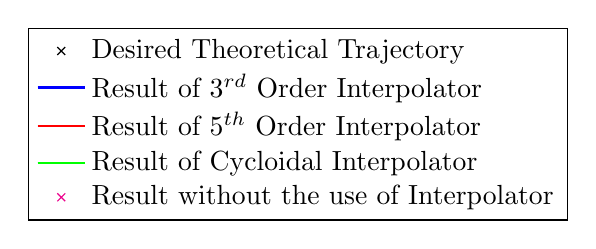
\begin{tikzpicture}
    \begin{customlegend}[legend entries={Desired Theoretical Trajectory,Result of $3^{rd}$ Order Interpolator,Result of $5^{th}$ Order Interpolator,Result of Cycloidal Interpolator,Result without the use of Interpolator},legend cell align=left]
    \addlegendimage{black,mark=x,only marks}   \addlegendimage{blue,fill=blue,thick,sharp plot}
    \addlegendimage{red,fill=blue,thick,sharp plot}
    \addlegendimage{green,fill=blue,thick,sharp plot}
    \addlegendimage{magenta,mark=x,only marks}
    \end{customlegend}
\end{tikzpicture}
\caption{Obtained trajectories with different interpolators}
\label{fig:trayint}
\end{figure}

It can be seen that the use of interpolators greatly improve the obtained results, and are able to more correctly approximate to the desired result, even with an open-loop control.

It should be noted that in the case of cycloidal interpolator, the point of reference was accidentally moved, and thus a circular trajectory was obtained, but it's center is not aligned with the rest of the trajectories.

%-------------------------------------------
\section{Conclusions}
%-------------------------------------------

This work had many objectives, all regarding the modeling and control of a simple two-wheeled mobile robot.
First, the kinematic analysis made by \cite{dudek_computational_2010}, for differential mobile robots, was studied and evaluated for a simple curved trajectory, and compared with experimental values.
 
Then, the dynamic model proposed by \cite{ivanjko_modelling_2010} was used for the same type of mobile robot.
Given the same trajectory, a number of interpolators were chosen, with the objective of verifying their characteristics and observing whether they improved the resulting trajectories.
Regarding these, the interpolators chosen are base on the most used in the studies of \cite{canini_controllo_2003}.
The observed results were highly favorable: even with an open-loop control, the use of interpolators seemed to reduce significantly errors in trajectories, caused mostly by mechanical or electro-mechanical parts.
Depending on the requirements of the robot, the user may be able to choose many of these different interpolators to obtain the desired result, for example a minimum RMS velocity (reducing the current and therefore energy consumption), minimizing sharp accelerations and jitter, etc.

These errors were also analyzed, since they were introduced by a combination of factors, most notably the quality of the mechanical pieces, the quality and repeatability of the electric motors, and the measurement quality of the optical encoders.

For future works, it is proposed to improve the control system used to move the robot.
Since, for budget reasons, the mechanical system would not be changed, what's left is to create more robust control systems, with the objective of reducing errors as much as possible.
The use of interpolators has already shown their feasibility in significantly reducing these errors, but more can be done to better the results, for example implementing the calibration factors obtained in the initial measurements, and designing closed-loop control systems, which would translate in a more robust scheme, with greater immunity to errors.

Finally, the project could be enhanced by adding more complex trajectories to the experiment, which would actually be variations of a fixed-radius circle.
The use of sensors for the trajectory decision/control could also be considered, in the case of distance sensors, position sensors, etc.
 
 %-------------------------------------------
\section{Thanks}
%-------------------------------------------
% las fuentes de financiación

The authors wish to thank the Electronics and Visual Learning Departments of "Universidad Tecnológica Nacional", for the purchase of these mobile robots, and laboratory equipment.
We would also wish to thank them for helping finance this publication, and allowing us to present it in various opportunities.

%.---------------------- 
 
\bibliography{biblio_template}
\end{document}

%.----------------------




